\documentclass{book}
%\usepackage{fancyvrb}
\usepackage{bm}
\usepackage{float}
\usepackage{amsmath}
\usepackage{amsfonts}
\usepackage{graphicx}
\usepackage{lineno}
\usepackage{natbib}
\usepackage[pdftex, pdfstartview=FitH,pdfpagemode=UseNone]{hyperref}
\usepackage{verbatim}
\usepackage{soul}
\usepackage{color}

\bibliographystyle{asa}

\floatstyle{plain}
\floatname{panel}{Panel}
\newfloat{algorithm}{h}{txt}[chapter]
\newfloat{panel}{h}{txt}[chapter]


\newcommand{\R}{\textbf{R}}
\newcommand{\bugs}{\textbf{BUGS}}
\newcommand{\jags}{\textbf{JAGS}}
\newcommand{\secr}{\mbox{\tt secr}}
\newcommand{\scrbook}{\mbox{\tt scrbook}}


\linenumbers

\begin{document}


\begin{comment}
  \part{Background and Concepts}


  \chapter{Introduction}
  \label{chapt.intro}

  \chapter{GLMS and WinBUGS}
  \label{chapt.glms}

  \chapter{Closed population models}
  \label{chapt.closed}

  \chapter{Fully Spatial capture-recapture models}
  \label{chapt.scr0}

  \chapter{MLE chapter}
  \label{chapt.mle}

  \chapter{Modeling Encounter Probability}
  \label{chapt.covariates}

  \chapter{Goodness of Fit and stuff}
  \label{chapt.gof}

  \chapter{Other observation models}
  \label{chapt.poisson-mn}

  \chapter{
Sampling Design
}
\markboth{Sampling design}{}
\label{chapt.design}

\vspace{.3in}


Statistical design is recognized as an important component of animal
population studies \citep{morrison_etal:2008,
  williams_etal:2002}. There are probably few to no field biologists
who have never been in the situation where a problem with data could
be traced back to some flaw in study design.  Commonly, design is
thought of in terms of number of samples to take, when to sample,
methods of capture, desired sample size (of individuals), power of
tests, and related considerations.  In the context of spatial sampling
problems, where populations of mobile animals are sampled by an array
of traps or devices, there are a number of critical design elements.
Two of the most important ones are the spacing and configuration of
traps (or sampling devices) within the array.  While conceptual and
heuristic design considerations have been addressed by a number of
authors (e.g., \citealp{nichols_karanth:2002}, Chapt. 11), little
formal analysis focused on spatial design of arrays has been carried
out. \citet{bondrup-nielsen:1983} investigated the effect of trapping
grid size (relative to animal home range area) on density estimates using a simulation
study and some authors have addressed trap spacing and configuration
by sensitivity ``re-analysis'' (deleting traps and reanalyzing;
\citealp{wegge_etal:2004, tobler_etal:2008}). The scarcity of
simulation-based studies looking at study design issues is surprising,
as it seems natural to evaluate prescribed designs by Monte Carlo
simulation in terms of their accuracy and precision.

Theoretically optimal (or extremely good) designs are useful to study
in order to understand how factors influence the design
problem. However, often field studies face logistic difficulties,
especially when dealing with wide-ranging, rare and cryptic species
like large carnivores. The need to sample large areas with limited
resources often forces researchers to compromise between a study
design that is optimized for statistical inference and a study design that is
logistically viable or efficient. In such studies, traps are often placed along
roads or rivers where a large number of traps can be accessed with
relative ease. Unless the study site is crossed by a network of roads
or waterways, this will lead to a sampling design that is much more
'linear' compared to an area-based design where traps are spread out
uniformly over the study site.

In this chapter we recommend a general framework for evaluating
specific design choices for SCR studies based on Monte Carlo
simulation of specific design scenarios based on trade-offs between
available effort, funding, logistics and other practical
considerations -- what we call {\it scenario analysis}.  Many study
design related issues such as how long to survey in order to obtain
sufficient data, can be addressed with preliminary field studies that
will give you an idea of how much data you can expect to collect
within a unit of effort (a camera trap day or a point count survey,
for example).  But it is also always useful to perform scenario
analysis based on simulation before conducting the actual field survey
not only to evaluate the design in terms of its ability to generate
useful estimates of things, but also so that you have an expectation
of what the data will look like as they are being collected. This
gives you the ability to recognize some pathologies and possibly
intervene to resolve issues before they render a whole study
worthless. Suppose you design a study to place 40 camera traps based
on your expectations of parameter values you obtained from a careful
review of the literature, and simulation studies suggest that you
should get 3-5 captures of individuals per night of sampling. In the
field you find that you're realizing 0 or 1 captures per night and
therefore you have the ability to sit down and immediately question
your initial assumptions and possibly take some remedial
action. Simulation evaluation of design {\it a priori} is therefore a
critical element of any field study.

%Yet another design that has been
%proposed for regular capture-recapture studies is that of a trapping
%web (DESCRIBE). {\bf XXXX Maybe not? XXXX} In the second part of this
%chapter we look into the performance of these trap arrangements.


While we recommend scenario analysis as a general tool to understand
your {\it expected data} before carrying out a spatial
capture-recapture study, it is possible to develop some heuristics and
even analytic results related to the
broader problem of model-based spatial design
\citep{muller:2007} using an explicit objective function based on the
inference objective.  We outline an approach in this chapter where we
identify a variance criterion that depends on the configuration of
trap locations, and we optimize that variance criterion over the
design space (the collection of all possible designs of a given
size). While there is much work to be done on developing this idea, we
believe that it provides a general solution to any type of design
problem where the space of candidate trap locations is well-defined. 
% XXXX RC says: I would beef this paragraph up. You write a lot about the
% simulation-based scenario-analysis, but just 1 sentence about the
% analytical approach which seems very promising.


% XXXX RC says: Doesn't Murray have some paper where he discuss design
% issues? Or where did the 2sigma rule come from? Also, you might want
% to cite Rahel/Beth's paper on design here.

\section{General Considerations}

Many biologists have experience with the design of natural resource
surveys from a classical perspective
\citep{thompson:2002,cochran:2007}, a key feature of which involves
sampling space. That is, we identify a sample frame comprised of
spatial units and we sample randomly (or by some other method, such as
generalized random tesselation stratified (GRTS) sampling \citep{stevens_olsen:2004})
those units and measure some attribute. The resulting inference
applies to the attribute of the sample frame. There are some distinct
aspects of the design of SCR studies which many people struggle with
in their attempts to reconcile SCR design with classical survey design
problems.

\begin{comment}
\subsection{Model-based not design-based}

{\bf XXX ANDY: I find this little subsection hard to understand; maybe it needs some mroe elaborating. I really like the following one though. XXXXXX

XXX Reply: Andy sez: I agree, not worth going here.
}
We take a model-based approach to the design of SCR studies. That is,
we seek design features -- spatial arrangements of samples -- which we
expect to produce estimators of model parameters that have a
satisfactory desired level of precision.

Classical finite-population sampling is often ``design-based'' which
means properties of estimators (bias, variance) are evaluated over
repeated realizations of the {\it sample}. The sample is random, but
the attribute being observed is not. However, in the SCR modeling
framework properties of our estimators are distinctly model-based.  We
evaluate estimators (usually) or care only about a {\it fixed} sample,
averaged over realizations of the underlying process and data we might
generate. This is a classical parametric frequentist idea which we
think makes as much sense as a Bayesian too.
\end{comment}



\subsection{Sampling space or sampling individuals?}

A fundamental question in any sampling problem is what is the sample
frame -- or the population we are hoping to extrapolate too. In the
context of capture-recapture studies, it is tempting to think of the
sample frame as being spatial (the space within ``the study area'',
tiled into quadrats perhaps).  Clearly SCR models involve a type of
spatial sampling -- we have to identify spatial locations for traps,
or arrays of traps.  However, unlike conventional natural resource
sampling the attribute we measure is {\it not} directly relevant to
the {\it sample location}, such as where we place a trap and,
therefore, it may not be sensible to think of the sample frame as
being comprised of spatial units.
% XXXX RBC says: I think it is worth discussing the situation in which
% a researcher wants to know density (or variation in density) within
% some well-defined area, like a park or on an island. In that case,
% they very well might want to think about sampling some finite
% space. RBC says later: Okay, see that you discuss this issue in
% depth below, but you might want to briefly say something about it
% here too XXXX
On the other hand,
capture-recapture studies clearly obtain a sample of {\it individuals}
and SCR models are models of {\it individual} encounter and space use.
Therefore, it is more natural to think of the sample frame as a list
of $N$ individuals, deterimined by the definition of the state-space,
or a subset of the state-space, i.e., the study-area, but the number
$N$ is unknown.
%You can think of it this way: the study
%area deterimines the collection of individuals that we care about for
%management or whatever, but additional individuals might be exposed to
%sampling.

Spatial sampling in SCR studies is important, but only as a device for
accumulating individuals in the sample from which we can learn about
their inclusion probability. That is, we're not interested in any
sample unit attribute directly but, rather, we use spatial units as a
means for sampling individuals and obtaining individual level
encounter histories.
It makes sense in this context
that we should want to choose a set of spatial sample units that
provides an adequate sample size of individuals, perhaps as many as
possible. The key technical consideration as it relates to spatial
sampling and SCR is that arbitrary selection of sample units has a
side-effect that it induces unequal probabilities of inclusion into
the sample and so we must also learn about these unequal probabilities
of sample inclusion as we obtain our sample.

The fact that SCR sampling induces unequal probabilities of sampling
is consistent with the classical sampling idea of Horvitz-Thompson
estimation (see
\url{http://en.wikipedia.org/wiki/Horvitz%E2%80%93Thompson_estimator})
which has motivated capture-recapture models similar to SCR
\citep{huggins:1989, alho:1990}.  In the Horvitz-Thompson framework,
the sample inclusion probabilities are usually fixed and
known. However, in all real animal sampling problems they are
unknown because we never know precisely where each individual lives
and therefore cannot characterize its encounter probability.
Therefore, we have to estimate the sample inclusion probabilities
using a model.  SCR models achieve this effect formally, using a
fully model-based 
approach based on a model that accounts for the
organization of individual activity centers and trap locations.
This notion of Horvitz-Thompson estimation suggests that perhaps we
should consider designing SCR studies based on the H-T variance
estimator as a design criterion. We discuss this a little bit later
in this chapter.

\subsection{Focal population vs. state-space}

In SCR models we make a distinction between the focal population --
the population of individuals we care about -- and those
of the state-space,
which we are required to prescribe in order to fit SCR models.
These are not the same thing. The geographic scopt of the population
of inference is
region within which animals live that you care about in your study --
let's call this ``the study area''.  This is often prescribed for
political reasons or legal reasons (e.g. a National Park). To intitiate a study, or perhaps
motivating the study, you have to draw a line on a map to delineate a
study area, although often it is difficult to draw this line, and
where you draw it is not so much a statistical/SCR issue.  On the
other hand, you need to prescribe the state-space to define and fit an
SCR model. This is the region that contains individuals that you {\it
  might} capture. This is different from the study area in most cases.
To design a study, you need a well-defined study area, but the
state-space will also be relevant to efficient distribution of traps,
and other considerations.

% XXXX RBC says: the next two paragraphs are great
It is helpful to think about this distinction operationally. We define
our study area a priori.  As a conceptual device, we might think of
this as the area that, given an infinite amount of resources, we might
wall-off so that we can study a real closed population. This 'study
area' should exist independent of any model or estimator of some
population quantity. i.e., the subject-matter context should determine
what the study area is. Given a well-defined study area, we use some
method to arrange data collecting devices within this study area. The
method of arrangement can be completely arbitrary but, naturally, we
want to choose arrangements of traps that are better in terms of
obtaining statistical information from the data we wind up collecting.

Lets face it -- It's quite a nuisance that animals move around and
this makes the idea of a spatial study area kind of meaningless in
terms of management in most cases. Wherever you draw a line on a map,
there will be animals who live mostly beyond that line that will
sometimes be subjected to your study.  One of the benefits of SCR
models is they formalize the exposure and contribution of these
individuals to your study. That is a good thing. Thus, you can
probably be a bit sloppy or practical in your definition of ``the
study area'' and not worry too much.



\section{Study design for (spatial) capture-recapture}

The importance of adequate trap spacing and overall configuration of
the trapping array has long been discussed in the capture-recapture
literature.  A heuristic based on recognizing the importance of
typical home range sizes \citep{dice:1938, dice:1941} and thus being
able to obtain information about home range size is that traps should
be spaced such that the array of available traps exposes as many
individuals as possible but, at the same time, individuals should be
captureable in multiple traps. Thus, good designs should generate a
high sample size $n$
(i.e., the number of individuals captured) % XXXX RBC add this
and a large number of spatial recaptures.  These
two considerations trade-off in building designs.  On one hand, having
a lot of traps very close together should produce the most spatial
recaptures but produce very few unique individuals captured (assuming
that studies are limited in the total number of sampling devices they
can deploy). On the other hand, spreading the traps out as much as
possible, in a nearly systematic or regular design, should yield the
most unique individuals.  We will formalize this trade-off later, when
we consider formal model-based design of SCR studies.


Traditional CR models require that all individuals in the study area
have a probability $>$ 0 of being captured, which means that the trap
array must not contain ``holes'' large enough to contain an animal's
entire home range \citep{otis_etal:1978}. This ``assumption'' is
imposed in order that a precise area can be used for defining the
population, and for calculation of density. 
% XXXX The non-spatial CR assumption of "no holes" should be
% emphasized heavily. I suggest adding a few sentence about why
% non-spatial models require this assumption, and what the
% consequences of violating it are. And then talk about how hard it is
% to enforce when studing big animals.
As a consequence, trap
spacing should be on the same order as the radius of a typical home
range (e.g., \citealp{dillon_kelly:2007}).  For example, imagine a
camera trap study implemented in South America with the objective to
survey populations of both jaguars and the much smaller
ocelots
({\it Leopardus pardalis}). % XXXX What's our policy on scientific names?
Ocelots also have much smaller home ranges and therefore
should require closer trap spacing than the large wide-ranging
jaguars.  Where approaches such as MMDM are used in combination with
traditional CR models to obtain density estimates (see
Chapt. \ref{chapt.closed}), trap spacing also has a major effect on
movement estimates, since it determines the resolution of the
information on individual movement \citep{parmenter_etal:2003,
  wilson_anderson:1985b}. If trap spacing is too wide, there is little
to no information on animal movement because most animals will only be
captured at one trap \citep{dillon_kelly:2007}. In addition, only a
trapping grid that is large relative to individual movement can
capture the full extent of such movements, and researchers have
suggested that the grid size should be at least four times that of
individual home ranges to avoid positive bias in estimates of density
\citep{bondrup-nielsen:1983}.  This recommendation originated in small
mammal trapping, and it should be relatively easy to follow when
dealing with species covering home ranges $<$ 1 ha. However, translated
to large mammal research, this can entail having to cover several
thousands of square kilometers -- a logistical and financial challenge
that few projects could realistically tackle.

Holes in the study area are of no concern in SCR studies.  As a
practical matter, some animals within the study area might have
vanishingly small probability of being included in the sample, i.e.,
$p \approx 0$, the nice thing about SCR models is that $N$ is
explicitly tied to the state-space, and not the traps which expose
them to encounter.  Within an SCR model, extending inference from the
sample to individuals that live in these holes represents an
extrapolation (prediction of the model outside the range of the data),
but one that the model is capable of producing because we have
explicit declarations, in the model, that it applies to any area
within the state-space (the state-space is a part of the model!), even
to areas where we can't capture individuals because we happened to not
put a trap near them. Conversely, ordinary capture-recapture models
only apply to individuals that have encounter probability that is
consistent with the model being considered. Presumably, the existence
of a hole in the trap array would introduce individuals with $p=0$,
which is not accommodated in those models.


Whereas traditional CR studies are concerned with the number of
individuals and recaptures and with satisfying the model assumption of
all individuals having some probability of being captured, in spatial
capture-recapture we are looking at an additional level of
information: We need spatially spread out captures and
recaptures. That means, it is not enough to recapture an individual,
but we need to recapture at least some individuals at several
traps. Therefore, in general, design of SCR studies boils down to
obtaining three bits of information: total unique
individuals captured,
total number of recaptures
informative about baseline encounter
rate, and spatial recaptures, informative about $\sigma$. Most SCR
design choices wind up trading these three things against each other
to achieve some optimal (or good) mix. So for example if we sample a
very small number of sites a huge number of times then we can get a
lot of recaptures but only very few spatial ones, and few unique
individuals etc.  This need for spatial recaptures may appear as an
additional constraint on study design, but actually, SCR studies are
much less restricted than traditional CR studies, because of the way
animal movement is incorporated into the model: $\sigma$ is estimated
as a specified function of the ancillary spatial information collected
in the survey and the capture frequencies at those locations and this
function is able to make a prediction across distances even when these
are latent, including distances larger than the extent of the trap
array. When there is enough data across at least some range of
distances, the model will do well at making predictions at unobserved
distances. The key here is that there needs to be `enough data across
some range of distances', which induces some constraint on how large
our overall trap array must be to provide this range of distances
(e.g., \citealp{marques_etal:2011}). We will review the flexibility of
SCR models in terms of trap spacing and trapping grid size in the
following section.


\section{Trap spacing and array size relative to animal movement}


% XXXX RBC says: Hard-core Bayesians might want you to say that you
% did a frequentist evaluation of a Bayesian estimator.
Using a simulation study, \citet{sollmann_etal:2012} investigated how
trap spacing and array size relative to animal movement influence SCR
parameter estimates and we will summarize their study here. They
simulated encounter histories on an $8 \times 8$ trap array with
regular spacing of 2 units, using a binomial 
observation model with
Gaussian hazard encounter model, across a 
range of values for the movement parameter $\sigma^*$. We refer to the
movement parameter as $\sigma^*$ here, because
\citet{sollmann_etal:2012} use a slightly different parametrization of
SCR models, in which $\sigma^*$ corresponds to $\sigma\times\sqrt{2}$.

{\bf XXXX ANDY: I am totally blanking here: We formulated the model so
  that the distance function was d2/sig2. That means $\sigma^*$ =
  $\sigma\times\sqrt{2}$, right? It was different before but I think
  now it's right. If I got it wrong, let me know and I'll fix
  it. Sorry!! XXXXXXXXXXXXXXXXXXXXXXXXXXXXXXXXXX }
{\bf XXX Andy sez: I think this is right!}

In Sec. \ref{scr0.sec.implied} we pointed out that under the bivariate
normal (or half-normal) detection model $\sigma$ can be converted into
an estimate of the 95 \% home range or ``use area'' around
$s_i$. Based on this transformation, values for $\sigma^*$ were chosen
so that there was a scenario where
the trap array was smaller than a single individual's home range,
i.e. trap spacing was narrow relative to individual movements
($\sigma^*$ = 5), a scenario where spaces between traps were large
enough to contain entire home ranges ($\sigma^*$ = 0.5), and two
intermediate scenarios and where sigma was smaller ($\sigma^*$ =1
unit) and larger ($\sigma^*$ = 2.5 units) than the trap spacing,
respectively.  $N$ was 100 and the baseline trap encounter rate
$\lambda_0$ was 0.5 for all four scenarios, and trap encounters were
generated over 4 occasions. Table \ref{design.tab.simres} shows the
results as the average over 100 simulations.

 \begin{table}[ht]
  \centering
  \caption{
Mean, relative root mean squared error (rrmse) of the mean, mode, 2.5
\% and 97.5 \% quantiles, relative bias of mean (RB) and 95\%BCI
coverage (BCI) for spatial capture-recapture parameters across 100
simulations for four simulation scenarios, define by the input value
of movement parameter $\sigma^*$. $N$ = number of individuals in the
state space; $\lambda_0$ = baseline trap encounter rate.}
    \begin{tabular}{l*{7}{c}}
    \hline
    Scenario & Mean  & rrmse & Mode  & 2.5\% & 97.5\% & RB    & BCI \\     \hline
    \multicolumn{2}{ l }{\bf $\sigma^*$ = 1 ($\sigma$ = 0.71)}  & {\it } & {\it } & {\it } & {\it } & {\it } & {\it } \\
    $N$ & 108.497 & 0.172 & 104.099 & 78.977 & 143.406 & 0.085 & 96 \\
    $\lambda_0$ & 0.518 & 0.248 & 0.477 & 0.303 & 0.752 & 0.035 & 94 \\
    $\sigma^*$ & 1.008 & 0.093 & 0.990 & 0.857 & 1.195 & 0.008 & 94 \\
    \multicolumn{2}{ l }{\bf $\sigma^*$ = 2.5 ($\sigma$ = 1.77)} & {\bf } & {\bf } & {\bf } & {\bf } & {\bf } & {\bf } \\
    $N$ & 100.267 & 0.105 & 98.456 & 82.086 & 121.878 & 0.003 & 97 \\
    $\lambda_0$ & 0.507 & 0.118 & 0.500 & 0.409 & 0.623 & 0.014 & 92 \\
    $\sigma^*$ & 2.501 & 0.046 & 2.491 & 2.267 & 2.690 & $<$ 0.001 & 92 \\
    \multicolumn{2}{ l }{\bf $\sigma^*$ = 5 ($\sigma$ = 3.54)} & {\bf } & {\bf } & {\bf } & {\bf } & {\bf } & {\bf } \\
    $N$ & 102.859 & 0.137 & 100.756 & 77.399 & 130.020 & 0.029 & 88 \\
    $\lambda_0$ & 0.505 & 0.075 & 0.501 & 0.435 & 0.580 & 0.011 & 93 \\
    $\sigma^*$ & 5.023 & 0.039 & 5.001 & 4.687 & 5.431 & 0.005 & 97 \\ \hline
    \end{tabular}
  \label{design.tab.simres}
\end{table}


\begin{table}[ht]
  \centering
  \caption{Summary statistics of 100 simulated data sets for four
    simulation scenarios, defined by the input value of movement
    parameter $\sigma^*$. Individual detection histories were
    simulated on an 8 x 8 trap array with regular trap spacing of 2
    units.}
    \begin{tabular}{l p{2.1cm} p{2.3cm}p{2.1cm}p{2.3cm}}
    \hline
    Scenario & Inds. \newline captured & Total \newline captures & Inds. \newline recaptured & Inds. captured  \newline at $>$ 1 trap \\ \hline
    {$\sigma^*$ = 0.5} & 18.29 (3.84) & 25.38 (5.86) & 5.52 (2.03) & 0.72 (0.95) \\
    {$\sigma^*$ = 1.0} & 37.70 (13.44) & 69.35 (26.05) & 19.48 (7.68) & 11.87 (5.43) \\
    {$\sigma^*$ = 2.5} & 44.19 (4.67) & 231.78 (33.98) & 36.60 (4.76) & 35.21 (4.73) \\
    {$\sigma^*$ = 5.0} & 40.51 (5.15) & 427.77 (79.09) & 33.09 (4.63)
    & 32.60 (4.76) \\ \hline
    \end{tabular}
  \label{design.tab.simdat}
\end{table}

All model parameters were
%%identifiable % XXXX RBC says: Suggest explaining what you mean by
             % identifiable here. Was the posterior the same as the prior?
%%% Andy edited: I removed this phrase
% and 
estimated with relatively
low bias ($<$ 10 \%) and high to moderate precision (RRMSE $<$ 25 \%)
for all scenarios of $\sigma^*$, except $\sigma^*$ = 0.5 units
(therefore excluded % XXXX RBC says: might be worth showing anyway
from Table \ref{design.tab.simres}). Data for the
latter case mostly differed from the other scenarios in that fewer
animals were captured and very few of the captured animals were
recorded at more than 1 trap (Table \ref{design.tab.simdat}). For
$\sigma^*$ = 0.5, abundance ($N$) was not identifiable in 88\% of the
simulations, and when identifiable, was underestimated by
approximately 50\%. This shows that a wide trap spacing that is
considerably too large may be problematic in SCR studies

Estimates (posterior means) % XXXX Posterior point estimates? XXX Andy
                            % added (posterior means) which he thinks
                            % is right.....
of $N$ were least biased and most precise under the
$\sigma^*$ = 2.5 scenario, and in general, all parameters were
estimated best under the $\sigma^*$ = 2.5 or the $\sigma^*$ = 5
scenario. All estimates had the highest relative bias and the lowest
precision under the $\sigma^*$ = 1 scenario.  These results clearly
demonstrate that SCR models can successfully handle a range of trap
spacing to animal movement ratios, and even when using a trapping
array smaller than an average home range: at $\sigma^*$ = 5, the home
range of an individual was approximately 235 $units^2$, while the
trapping grid only covered 196 $units^2$. Still, the model performed
very well.

An important consideration in this simulation study is that all but
the $\sigma^*$ = 0.5 units scenarios provided reasonably large amounts
of data, including 20 + individuals being captured on the trapping
grid. When dealing with real-life animals that are often territorial
and may have lower trap encounter rates, a very small grid compared to
an individual's home range may result in the capture of few to no
individuals. In that case, the sparse data will limit the ability of
the model to estimate parameters \citep{marques_etal:2011}, which is true
of most models.


To further explore
the effects of %the relationship between
trap spacing and movement
on %on one hand, and
bias and precision of estimates of $N$,  %on the other hand,
we expanded %a modified version of
the simulation study of %by
\citet{sollmann_etal:2012}: we considered a regular $7 \time 7$ grid,
with trap spacing ranging from $0.5 \times \sigma$ to $4 \times
\sigma$. XXXXX ANDY:SIMULATION DETAILS XXXXX. For each trap spacing
scenario we simulated and analyzed 500 data sets and calculated the
RRMSE
and relative bias for the estimates of $N$. Figure
\ref{design.fig.rmse} shows the results of this set of simulations. We
see that there is clearly an optimal
trap spacing, especially in terms
of precision, which is highest at a trap spacing of $1.5 - 2.5 \times
\sigma$. \citet{efford:2012wbbw} 
reported similar results and highlighted the
trade-off between the number of individuals captured 
and
the number of spatial recpatures 
-- intuitively, the former goes up with an increase in trap spacing,
whereas the latter goes down. In summary, in small trap spacing
scenarios, the small sample size leads to imprecise estimates, whereas
in large trap spacing scenarios, lack of spatial recaptures leads to
imprecise and biased estimates.

\begin{figure}[ht]
\centering
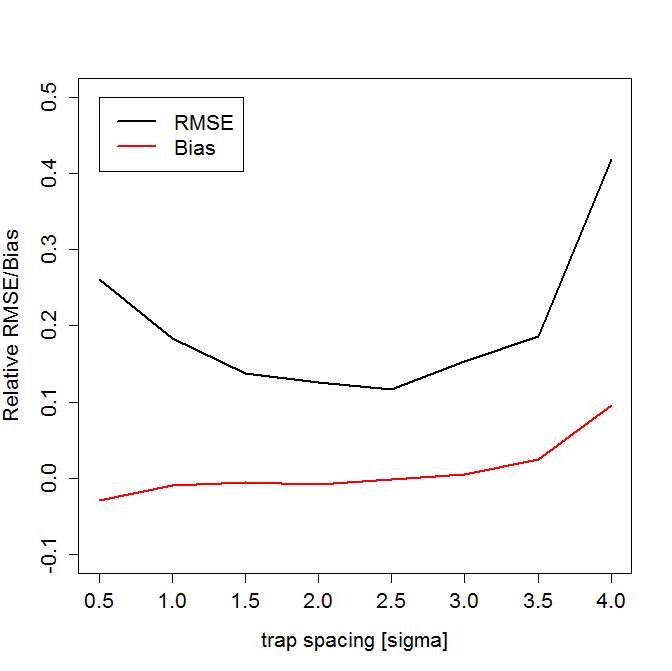
\includegraphics[width=3in]{Ch10-Design/figs/RMSE.png}
\caption{Fort Drum Black bear study area and the 38 baited hair snare
  locations operated for 8 weeks during June and July, 2006.}
\label{design.fig.rmse}
\end{figure}



% In summary, SCR models performed best when $\sigma^*$ was slightly
% larger than trap spacing (or in other words, when $\sigma$ was
% slightly smaller) and did well as long as $\sigma^*$ was at least 0.5
% times the average distance between traps (which corresponds to
% $\sigma$ being 0.35 times the average distance between
% traps). Although at this trap spacing to movement ratio, most
% individuals are captured at one trap only (see
% Tab. \ref{design.tab.simdat}), parameter estimates exhibited low bias
% and remained relatively precise (see simulation results for $\sigma^*$
% = 1 in Tab. \ref{design.tab.simres}). Below this trap spacing to
% movement ratio the spatial information in the simulated data
% apparently was not sufficient to inform SCR model parameters.


\subsection{Example: Black bears from Pictured Rocks National Lakeshore }

To see how trap array size influences parameter estimates from spatial
capture-recapture models in the real world, \citet{sollmann_etal:2012}
also looked at a black bear data set from Pictured Rocks National
Lakeshore, Michigan, collected using 123 hair snares distributed over
an area of 440 $km^2$ along the shore of Lake Superior in May-July
2005 \citep{belant_etal:2005}.  The SCR model for the bear data
included sex-specific
encounter rate parameters, and an occasion-specific baseline encounter
rate.
%and
%$\sigma^*$ between males and females, and $\lambda_0$ varied across
%occasions.
This was motivated by a) the lower average number of
detections for male bears, b) the decreasing number of detections
over time in the raw data, and c) the fact that male black bears are
known to move over larger areas than females (e.g.,
\citealp{gardner_etal:2010jwm, koehler_pierce:2003}).

To address the impact of a smaller trap array on the parameter
estimates, models fitted to the full data set were compared to
models fitted to data subsets.
The first subset retained only those 50\% of the traps
closest to the grid center. In the second, only the southern 20\% of
the traps were retained \ref{design.tab.bears}.

\begin{table}[ht]
  \centering
  \caption{Posterior summaries of SCR model parameters for black
    bears, modified from \citet{sollmann_etal:2012}.}
    \begin{tabular}{lcccc}
%    \addlinespace
	\hline
          & Mean (SE) & Mode  & 2.5\% & 97.5\% \\ \hline
    {\bf Full data set} &       &       &       &       \\
    {\it D } & 10.556 (1.076) & 10.448 & 8.594 & 12.792 \\
    $\sigma^*$ (males) & 7.451 (0.496) & 7.323 & 6.579 & 8.495 \\
    $\sigma^*$ (females) & 2.935 (0.143) & 2.939 & 2.671 & 3.226 \\
    {\bf 50\% of traps} &       &       &       &      \\
    {\it D } & 12.648 (1.838) & 12.205 & 9.307 & 16.713 \\
    $\sigma^*$ (males)  & 5.354 (0.511) & 5.248 & 4.472 & 6.473  \\
    $\sigma^*$ (females) & 3.318  (0.277) & 3.262 & 2.841 & 3.910 \\
    {\bf 20\% of traps} &       &       &       &        \\
    {\it D } & 6.752 (1.611) & 5.953 & 4.000 & 10.218  \\
    $\sigma^*$(males)  & 9.881 (3.572) & 7.566 & 5.121 & 18.447 \\
    $\sigma^*$ (females)  & 2.686 (0.391) & 2.657 & 2.121 & 3.404  \\
    \hline
    \end{tabular}
  \label{design.tab.bears}
\end{table}

Reducing the area of the trap array by 50\% created a grid polygon of
144 $km^2$, which was smaller than an estimated male black bear home
range and only 50\% larger than a female black bear home range --
approximately 260 $km^2$ and 100 $km^2$, respectively, when converting
estimates of $\sigma^*$ to home range size. Table
\ref{design.tab.bears} shows that this did not greatly influence model
results, compared to the full data set. The observed smaller
differences in parameter estimates may be due to individual
differences in detection and movement that manifest themselves when
only a smaller portion of the overall population is sampled. By
reducing the number of traps we effectively reduced the size of the
overall data set estimates were based on (both in terms of individuals
captured and recaptures).
% XXXX RBC says: the previous 2 sentences were not so clear.
This was reflected in overall higher SE and
wider confidence intervals. In spite of these differences, density
estimates %-\226 the main objective of applying SCR models -�
%remained largely constant.
were similar.
Removing 80\% of the traps and thereby % XXXX begin new paragraph?
reducing the area of the trap array to 64 $km^2$ -- well below the
average black bear home range -- had a great effect on sample size
(only 25 of the original 83 individuals sampled) and parameter
estimates. Particularly, male black bear movement was overestimated
and imprecise. The combination of the low baseline trap encounter rate
of males and the considerable reduction in sample size led to a low
level of information on male movement: 5 of the 12 males were captured
at one trap only. Although they moved over smaller areas, owing to
their higher trap encounter rate females were, on average, captured at
more traps (3.4 traps per individual compared to 2.6 for males) so
that their movement estimate remained relatively
accurate. Overestimated male movements and female trap encounter rates
resulted in an underestimate of density of almost 40\%. This effect
is contrary to what we would expect to see in non-spatial CR models,
where too small an area % XXXX RBC says: this isn't so clear. Do you
                        % mean, using an ad hoc value of effective
                        % sample area that is too small?
leads to underestimated movement and
overestimated density \citep{bondrup-nielsen:1983, dillon_kelly:2007,
  maffei_noss:2008}. While this example again demonstrates the ability
of SCR models to deal with a range of trapping grid sizes, it also
clearly shows that your study design needs to consider the amount of
data you can expect to collect.

\subsection{Summary thoughts on trap spacing and array size in SCR models}
% XXXX RBC says: In what way is this "final"?
%XXX Andy: I changed the heading but that doesn't resolve the problem
% XXX Maybe we need to rethink the intent of this subsection

When designing a capture-recapture study for a single species, trap
spacing and the size of the array can (and should) be tailored to the
spatial behavior of that species to ensure adequate data
collection. However, some trapping devices like camera traps may
collect data on more than one species and researchers may want to
analyze these data, too. Independent of the trapping device used,
study design will in most cases face a limit in terms of the number of
traps available or logistically manageable. As a consequence,
researchers need to find the best compromise between trap spacing and
the overall grid area. In the following sections we consider both
practical approaches to this trade-off and a model-based approach to
derive such an optimal study design.

Particularly for large mammal research, SCR models have much more
realistic requirements in terms of area coverage than non-spatial CR
models, under which density estimates can be largely inflated with
small trapping grids relative to individual movement
\citep{maffei_noss:2008}.
% XXXX RBC says: I agree with this previous sentence, but I'm not sure
% tha tthe reader fully understands why this is so, at this point.
How large the spatial survey effort needs to
be does not only depend on the extent of movement of the target
species, but also on the temporal effort, density and detection
probability \citep{marques_etal:2011} -- in summary, the amount of
data that can be collected with any given trap array. For low-density
species, like the black bears in the above example, small trapping
grids bear % XXXX No pun intended!?
the risk of not collecting enough data for parameter
estimation. Simulation studies can help you assess how effective a
certain study design is given a set of parameters. Alternatively,
\citet{efford_etal:2009ecol} provide a mathematical procedure to
determine the expected number of individuals captured and recaptures
for a given detector array and set of model parameters.
% XXXX Perhaphs efford_etal:2009ecol should have been mentioned earlier

% XXXX RBC says: This paragraph seems pretty redundant with previous material
Overall, while there are limits to the flexibility in spatial trap
array design for SCR modeling, the method is fairly robust to changes
in trap array size and spacing relative to animal movement. Trapping
grids with an extent of approximately a home range diameter can, %�
in theory, %-
adequately estimate density and home range size. However,
these results should not encourage researchers to design non-invasive
trap arrays based on minimum area and spacing requirements. Study
design should still strive to expose as many individuals as possible
to sampling and obtain adequate data on individual movement. Large
amounts of data do not only improve precision of parameter estimates
(the density estimate for the full black bear data set has narrower
confidence intervals than estimates from the reduced data sets), they
also allow including potentially important covariates (such as gender
or time effects in the black bear example) into SCR models to obtain
density estimates that reflect the actual state of the studied
population.



\section{Sampling Over Large Areas}

Trap spacing is an essential aspect of design of SCR studies. However,
it is only the most important aspect if one can uniformly cover a
study area with traps.   In many practical situations where the study
area is large relative to effort that can be expended, one has to
consider other strategies which deviate from a strict focus on trap
spacing. There are two general strategies that have been suggested
which we think are useful in practice, either by themselves or
combined: Sampling based on {\it clusters} of traps and sampling based
on {\it rotating} groups of traps over the landscape.

\citet{karanth_nichols:2002} describe 3 approaches of moving traps to
achieve coverage of a larger study area, geared towards traditional
capture-recapture analysis. Say, to sample the entire area of interest
requires sampling $J$ sites.

{\flushleft \bf (1)} For every day/sampling occasion, randomly choose
$x$ out of your $J$ sites, where $x$ is the number of trapping devices
you have at hand. Obviously, this requires the logistics of moving
traps to be quite easy.  \newline
{\flushleft \bf (2)} Move blocks of traps
that are close to each other in space daily. For example, if you
divide your total study area into 4 blocks, sample block 1 for a day,
then move traps to block 2 for a day, and so forth, and repeat until
each block has been sampled for a sufficient amount of time. \newline
{\flushleft \bf (3)} If moving blocks of traps daily is too
challenging, logistically, then you can sample each block for a
certain number of days/occasions before moving cameras to the next
block. In this fashion, you only need to move traps to each block
once.

In traditional CR we collapse data across traps and assume all
individuals in the study area have some probability $>0$ of being
detected. For our data that means that, under scenario (2) the first
occasion is defined as the time it takes to sample all 4 blocks once,
the second occasion consists of the second round of sampling all
blocks, etc. Under scenario (3), we have to combine data from day 1 in
each of the blocks to form occasion 1, data from day 2 in each of the
blocks forms occasion 2, and so on. Especially scenario 3 makes
modeling time-dependent detection difficult, since occasion 1 does no
longer refer to an actual day or continuous time interval.
We do not have that problem in SCR, where accounting for trap site
specific sampling effort is straight forward, as we first demonstrated
for the wolverine example in Sec. \ref{scr0.sec.wolverine}. Because we
are dealing with detection at the trap level, even for design (3) in a
spatial framework, we can still look at variation in detection over
time. As such, we don't think that one of the above designs is
superior for SCR models than the other, but rather, all of them will
produce adequate SCR data, as long as overall sample size requirements
are met.

\citet{efford_fewster:2012} looked at the performance of different
spatial study designs for abundance estimation from traditional and
spatial capture-recapture models, including a clustered design, where
groups of detectors are spaced throughout the larger region of
interest. They found that this design performed well, although there
were indications of a slight positive bias in estimates of $N$. Such a
clustered design enables researchers to increase area coverage without
having to increase the number of traps. \citet{efford_fewster:2012}
note that distribution of clusters has to be spatially representative
-- for example, systematic with a random origin. 
\citet{efford_etal:2009ecol} suggest a clustered type of design for
acoustic detectors (see Chapt. \ref{poisson-mn.sec.acoustic}, suggesting a design comprised of multiple small
(e.g., $2 \times 2$) clusters distributed in a probabilistic fashion
across the region of interest.
The issue of
spatially representative designs is not limited to SCR and an
extensive treatment of the topic can be found in the distance sampling
literature \citep{buckland_etal:2001}. Further, the authors stress
that, if distances among clusters are large and individuals are
unlikely to show up in several clusters, then the method relies on
spatial recaptures {\emph within} clusters, meaning that spacing of
detectors within clusters has to be appropriate to the movements of
the species under study.

In practice, employing both of these strategies -- clustering and
rotating traps -- might be necessary or advantageous. Especially for
clustered designs, further research on optimal detector configurations
is called for \citep{efford_fewster:2012}. More generally, work on
formalizing and generalizing these ideas of spatial study design is
needed.  We believe the model-based spatial design approach, which we
introduce below, is the way to do that.


\citet{sun:2013} used a simulation study to investigate different trap
arrangements (Fig. \ref{design.fig.sun}) for a black bear study based
on hair snares distributed over 2625 km$^2$ study area. She simulated
populations of bears for 3 trap arrangements including a regular
(uniform) coverage of traps, clusters of size 4 traps each with a gap
between clusters, and a design in which the clusters of size 4 were
moved mid-way through the study to fill the gap (we'll call this a
``rotating'' design).  She found that the precision and accuracy of of
$N$ estimates generally decreased when changing from uniform to
cluster to rotating design.


\begin{figure}[ht]
\centering
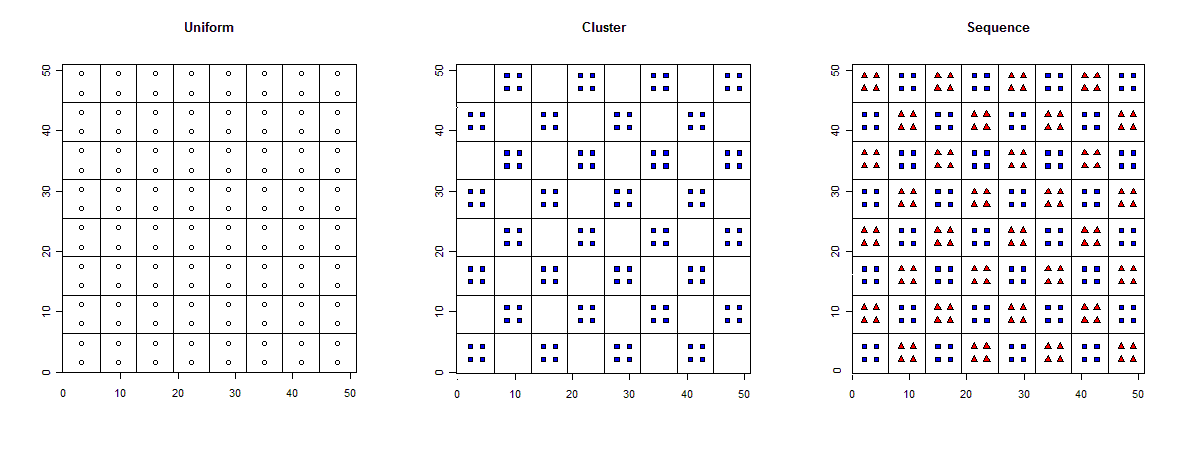
\includegraphics[width=5in,height=1.94in]{Ch10-Design/figs/catsun_designs.png}
\caption{Three designs evaluated by Sun XXXXX.  }
\label{design.fig.sun}
\end{figure}





\section{Model-Based Spatial Design}

A point we have stressed in previous chapters is that SCR models are
basically glorified versions of generalized linear models (GLMs) with
a random effect that represents a latent spatial attribute of
individuals, the activity center or home
range center.  This formulation makes analysis of the models readily
accessible in freely available software and also allows us to adapt
and use concepts from this broad class of models to solve problems in
spatial capture recapture. In particular, we can exploit
well-established model-based design concepts 
\citep{kiefer:1959,
box_draper:1959,
box_draper:1987,
fedorov:1972,
sacks_etal:1989,
hardin_sloane:1993,
fedorov_hackl:1997}
to develop a framework for designing
spatial trapping arrays for capture-recapture studies.
\citet{muller:2007} provides a recent monograph level treatment of the subject
that is very accessible.

In the following sections, we adapt these classical methods for
constructing optimal designs to obtain the configuration of traps (or
sampling devices) in some region (the design space, ${\cal X}$), that
minimizes some appropriate objective function based on a compromise
between the variance of estimating $N$ for a prescribed
state-space. We show that this criterion -- based on the variance of
an estimator of $N$ -- represents a formal compromise between
minimizing the variance of the MLEs of the detection model parameters
and obtaining a {\it high} expected probability of capture.
Intuitively, if our only objective was to minimize the variance of
parameter estimates than all of our traps should be in one or a small
number of clusters where we can recapture a small number of
individuals many times each. Conversely, if our objective was only to
maximize the expected probability of encounter then the array should
be highly uniform so as to maximize the number of individuals being
exposed to capture.  By seeking to minimize the variance of of an
estimator of $N$, our objective function is, formally, a compromise
between these two objectives and the resulting designs are not always
highly regular nor clustered.

% Existing theory (Sanathanan 1972) suggests that such designs
%should also be optimal for estimating density or abundance.

\subsection{Formalization of the Design Problem for SCR Studies}

Let ${\cal X}$, the {\it design space}, denote some region within
which sampling could occur and let ${\bf X} = {\bf x}_{1},\ldots, {\bf
  x}_{J}$ denote the {\it design}, the set of sample locations (e.g.,
of camera traps), normally we just call these ``traps.''  The design
space ${\cal X}$ must be prescribed (a priori).  Operationally, we
could equate ${\cal X}$ to the study area itself (which is of
management interest) but, in practical cases, there will be parts of
the study area that we cannot sample. Those areas need to be excluded
from ${\cal X}$.  While ${\cal X}$ may be continuous, in practice it
will be sufficient to represent ${\cal X}$ by a discrete collection of
points which is what we do here.  This is especially convenient when
the geometry of ${\cal X}$ is complicated and irregular, which would
be the case in most practical applications).  The technical problem
addressed subsequently is how do we choose the locations ${\bf X}$ in
a manner that is statistically efficient for estimating abundance or
density, or perhaps some other variance-based criterion?

As usual, we regard the population of $N$ such individual ``activity
centers'' as the outcome of a point process distributed independently
over the state-space ${\cal S}$.  The relevance and importance of
${\cal S}$ has been established repeatedly in this book, as it 
defines a population of individuals (i.e., activity
centers) and, in practice, it is not usually the same as ${\cal X}$
due to the fact that animals move freely over the landscape and the
location of traps is typically restricted by policies, ownership and
other considerations.  The objective we pursue here is: Given (1)
${\cal X}$, (2) a number of design points, $J$; (3) the state-space
${\cal S}$, and (4) an SCR model, and (5) a design criterion $Q({\bf
  X})$, we want to choose {\it which} $J$ design points we should
select in order to obtain the {\it optimal} design under the chosen
model, where the optimality is with respect to $Q({\bf X})$. We will
describe some possible choices for $Q({\bf X})$ below, but it makes
sense that they should relate to the variance of estimators of one or
more parameters of the SCR model.

To motivate the approach we're going to take in a simplified situation,
suppose for the moment that we know ${\bf
  s}$ for a single  individual.  In this case, its vector of counts of
encounter in each trap ${\bf y}$ are either binomial or Poisson
counts, and the model has this form:
\begin{equation}
g( \mathbb{E}({\bf y})  ) =  \alpha_0  + \alpha_1 ||{\bf x}-{\bf s}||^2.
\label{eq.linearpredictor}
\end{equation}
Or based on some other encounter probability model. In vector form we
write this as:
\[
g( \mathbb{E}({\bf y})  ) =  {\bf M}'{\bm \alpha}
\]
where ${\bf M}$ is the $J \times 2$ design matrix where the 2nd column
contains the squared pairwise distances between each individual $i$
and trap $j$, and thus it depends on both ${\bf X}$ and ${\bf s}$.  A
simpler model is the normal linear model, of the form:
\[
{\bf y} = {\bf M}({\bf X},{\bf s})'{\bm \alpha} + \mbox{error}
\]
The variance-covariance matrix of $\hat{\bm \alpha}$ is, supressing
the dependence on ${\bf X}$, 
\[
 \mbox{Var}( {\bm \alpha},{\bf X}) = ({\bm M}({\bf s})'{\bm M}({\bf s}))^{-1}
\]
Note that the design points ${\bf x}_{j}$ appear explicitly (in the
2nd column of {\bf M}).  In considering design for estimation in such
models it is natural to choose design points, corresponding to values
of ${\bf x}$, such that the variance of $\hat{\bm \alpha}$ is
minimized.  In particular, for a population of $N$ individuals, if we
know {\it all} $N$ values of ${\bf s}$ we could now easily find the
design ${\bf X}$ that optimizes some function of the
variance-covariance matrix, whatever function we want.  If we don't
know ${\bf s}$ then we might consider minimizing  the expected variance:
\[
  E_{{\bf s}}\left\{ \mbox{Var}({\bm \alpha},{\bf X}) \right\} = \sum_{s \in
    {\cal S}}  ({\bf M}'({\bf s}){\bf M}({\bf s}))^{-1}
\]
but this is not the expected variance based on sampling a population of $N$
individuals, just for a single individual having unknown ${\bf
  s}$. Because of the matrix inverse in this expression, it is not
sufficient to use a variance criterian that weights this variance by
$N$ or even the expected sample size. 
As an alternative, 
we can maximize the expected {\it information} which is probably more
appealing from an analytic point of view.
The information matrix is:
\[
 \mbox{Inf}({\bm \alpha},{\bf X}) = 
 ({\bf M}'({\bf s}){\bf M}({\bf s}))
\]
and, for a population of individuals, let ${\bf M}_{i}$ be the design
matrix for individual with 
activity center ${\bf s}_{i}$, the total information is:
\[
 \mbox{Inf}({\bm \alpha},{\bf M}_{1},\ldots,{\bf M}_{N}) = 
 \sum_{i=1}^{N}  ({\bf M}_{i}'({\bf s}_{i}){\bf M}_{i}({\bf s}_{i}))
\]
Now, because we don't know ${\bf s}_{i}$ we can compute the integrated
information, over all possible values of ${\bf s}_{i}$, and for {\it
  each} ${\bf s}_{i}$, which is an $N$-fold summation:
\[
E_{ {\bf s}_{1}, \ldots, {\bf s}_{N}}
\left\{  \mbox{Inf}({\bm \alpha},{\bf M}_{1},\ldots,{\bf M}_{N}) \right\} = 
 \sum_{i=1}^{N}  \sum_{s \in {\cal S}} ({\bf M}_{i}'({\bf s}_{i}){\bf M}_{i}({\bf s}_{i}))
\]
which, if the activity centers are independent, is just $N$ copies of
the integrated (spatially averaged) information:
\[
E_{ {\bf s}_{1}, \ldots, {\bf s}_{N}}
\left\{  \mbox{Inf}({\bm \alpha},{\bf M}_{1},\ldots,{\bf M}_{N}) \right\} = 
N  \sum_{s \in {\cal S}} ({\bf M}_{i}'({\bf s}_{i}){\bf M}_{i}({\bf s}_{i})).
\]

It therefore seems sensible to 
 base design of SCR studies on some criterion that is a
function of this  integrated information matrix. E.g., maximize the diagonals, or the determinant.
This can be done for any number of design points ${\bf x}_{1},\ldots,
{\bf x}_{J}$ using standard exchange algorithms
\citep[see][Chapt. 3]{muller:1997} and we discuss this below
in Sec. \ref{design.sec.exchange}.
%which always improve the criterion but will not necessarily yield {\it
%  the} optimal design. 

It is worth noting that asymptotic formulae for
$\mbox{Var}( {\bm \alpha})$ can be cooked up for any type of GLM.
For the Poisson GLM, the asymptotic
variance-covariance matrix of $\hat{\bm \alpha}$, considering a single
individual having location ${\bf s}$, is\footnote{ e.g., see
  some appendix in the back of McCullogh and Nelder XXXXX or Agresti XXXX for
  example -- this is basic GLM theory that derives from the fact that
  the Poisson is a member of the natural exponential family of
  distributions.}
\begin{equation}
  \mbox{Var}(\hat{\bm \beta}|{\bf X},{\bf s}) 
=  ({\bf M}({\bf s})' {\bf D}({\bm \beta},{\bf s}){\bf M}({\bf s}))^{-1}.
\label{eq.varbeta}
\end{equation}
This is a 
 function of the design ${\bf X}$ as well as ${\bf s}$ both of which
 are balled-up in ${\bf M}$ --
the regression design matrix, and the matrix ${\bf D}$ which is a diagonal
matrix having elements $\mbox{Var}( y_{j}|{\bf s}) = \exp({\bf
  m}'{\bm \beta})$ for $y_{j}$ the frequency of encounter in trap $j$.

To summarize the main point: If we know where the guys live, we can
pick he optimal design directly. But we don't! So what do we do?




\subsection{An Optimal Design Criterion for SCR}

There are a number of appealing directions to pursue for deriving a
variance-based criterion upon which to devise designs for capture
recapture studies.  For one, we could formulate the problem as a
Huggins-Alho type of problem and follow along their analysis for
computing variances, and that might be fruitful. But the calculus is
a bit tedious for that.  Instead, a more fruitful area is to consider
the MLEs based on the marginal  Poisson or Binomial likelihoods, and then we
could possibly compute the variance-covariance matrix of the MLEs
directly.  This merits further investigation.   We take an easier
approach here, for illustrative purposes, devising 
a variance criteria based on
a conditional estimator of $N$ of the form
\[
  \tilde{N}  =  \frac{n}{\bar{p}}
\]
where $\bar{p}$ is the probability that an individual appears in the
sample of $n$ unique individuals. In SCR models an individual with activity center
${\bf s}_{i}$ is captured if it is
captured in {\it any} trap and therefore, under the Bernoulli model,
\[
 \bar{p}({\bf s}_{i}, {\bf X}) = 1 - \prod_{j=1}^{J} (1- p_{ij}({\bf
   x}_{j}, {\bf s}_{i}))
\]
and, under the Poisson model, we have:
\[
 \bar{p}({\bf s}_{i},{\bf X}) = 1 -  \exp(-\lambda_{0} \sum_{j}
 \exp(\beta* d({\bf x}_{j}, {\bf s}_{i})^2 ))
\]
where here we emphasized that this is conditional on ${\bf s}_{i}$ and
also the design -- the trap locations ${\bf x}_{j}$.
 The {\it
  marginal} probability of encounter, averaging over all possible
locations of ${\bf s}$ is:
\begin{equation}
 \bar{p}({\bf X}) = 1 - \int_{\bf s}    \bar{p}({\bf s}_{i},{\bf X})    d{\bf s}.
\label{design.eq.pbar}
\end{equation}
It is important to note that this can be calculated directly {\it
  given} the design ${\bf X}$. This is handy because we see that it is
used in the variance formulae given subsequently.

The approach we take here is we develop the variance of $\tilde{N}$
conditional on knowing the locations of all $N$ individuals and then
we suggest to unconditon on the realized point process by taking a
Monte Carlo average over realizations of ${\bf s}$ under a suitable
model for ${\bf s}$. The variance criterion we propose here is based
on a delta approximation $Var(n/\bar{p})$:
\begin{equation}
 Var(\tilde{N}(\bm \alpha) ) =
\frac{N^{2} Var(\bar{p})}{\bar{p}^{2}}  + N\frac{(1-\bar{p})}{\bar{p}}
\label{design.eq.theQ}
\end{equation}
This is a really intuitive-looking criterion upon which to base
designs. In particular, it is the sum of two components
which are
essentially those due to (1) estimation of $\bar{p}$ from the sample
and (2) the variance of $n$. We see that generally this criterion is improved
(decreases) as we do a better job estimating $\bar{p}$ and also as $n$
approaches $N$, i.e., as $\bar{p}$ increases to 1. Thus, good designs
should generate information about detection probability {\it and}
produce large samples of individuals.  The other way to look at this
is that the variance of estimating $N$ is due to the variance of
estimating $\bar{p}$ with a {\it penalty} due to have a low value of
$\bar{p}$ (the 2nd term being the penalty, which increases as
$\bar{p}$ goes to 0).  We suggest, therefore, that designs for
capture-recapture studies should seek to minimize
Eq. \ref{design.eq.theQ}, or perhaps generalizations of this to
account for other features of the model.



In order to work with this expersssion we will
have to do some analysis of $\mbox{Var}(\bar{p})$ which we take up now.
We note that $\bar{p}$ is itself a deterministic function of the
parameters that we need to estimate, ${\bm \alpha}$. Therefore, as a
general rule,  we could use
a delta approximation to  express $\mbox{Var}(\bar{p})$ in terms of the variance of
the MLE $\hat{\bm \alpha}$.  However, we stated above that our intent
is to work with the Poisson observation model, and we did that because
the technical argument that follows is somewhat easier for that
case. In particular, we first express the integral in Eq.
\ref{design.eq.pbar} by a summation over a fine mesh of points so that:
\[
 \bar{p}({\bf X}) = \sum_{{\bf s}} 1 -    \bar{p}({\bf s}_{i},{\bf X})
\]
which under the Poisson model is, in a simplified notation:
\[
 \bar{p}({\bf X}) = \sum_{{\bf s}} \left\{
1 -  \exp(-\lambda_{0} \sum_{j}
 exp(\beta* d({\bf x}_{j}, {\bf s})^2))
\right\}
\]
To compute the variance of this expression, we note that the variance
operature can move inside the summation over ${\bf s}$, and the
subtraction from 1 doesn't count anything, so we have
\[
Var( \bar{p}({\bf X}) )  = \sum_{{\bf s}}
 Var \left(
 \exp(-     \sum_{j}   exp(\alpha_{0} + \alpha_{1}  d({\bf x}_{j}, {\bf s})^2))
   \right)
\]
At this point we apply the Delta approximation to produce
\[
Var( \bar{p}({\bf X}) )  = \sum_{{\bf s}}
\left( exp( - \sum_{j} exp(\alpha_{0} + \alpha_{1}  d({\bf x}_{j}, {\bf  s})^2) )
\right)
 Var \left(    \sum_{j}   exp(\alpha_{0} + \alpha_{1}  d({\bf x}_{j}, {\bf     s})^2)    \right)
\]
we're going to simplify things a bit and write $\lambda({\bf
  x}_{j},{\bf s}) =   exp(\alpha_{0} + \alpha_{1}  d({\bf x}_{j}, {\bf
  s})^2)$
and also $\lambda_{\bf s} = \sum_{j=1}^{J} \lambda({\bf x}_{j},{\bf
  s})$. Then
\[
Var( \bar{p}({\bf X}) )  = \sum_{{\bf s}}
\left( exp( - \lambda_{\bf s} )  \right)
 Var \left(    \sum_{j}   exp(\alpha_{0} + \alpha_{1}  d({\bf x}_{j}, {\bf     s})^2)    \right)
\]
We have to do a 2nd application of the Delta approximation to find
that:
\[
Var( \bar{p}({\bf X}) )  =
\sum_{{\bf s}} \left( exp( - \lambda_{\bf s} )  \right)
\left(    \sum_{j}  \lambda({\bf x}_{j},{\bf s})^{2} Var( \hat{\alpha}_{0} + \hat{\alpha}_{1}  d({\bf x}_{j}, {\bf    s})^2)
  \right)
\]
(note: need to comment on why $\alpha$ has hats on it somewhere but
not elsewhere)
The final step is we assume $\hat{\alpha}_{0}$ and $\hat{\alpha}_{1}$
are independent which is not true in practice but makes life slightly
easier here (but is not necessary, in general). The variance of
$\bar{p}$ becomes:
\[
Var( \bar{p}({\bf X}) )  =
\sum_{{\bf s}} \left( exp( - \lambda_{\bf s} )  \right)
\left(    \sum_{j}  \lambda({\bf x}_{j},{\bf s})^{2} (
 Var( \hat{\alpha}_{0}) +
  d({\bf x}_{j}, {\bf    s})^4
Var( \hat{\alpha}_{1})  )
  \right)
\]



The big picture is this: For a given design ${\bf X}$, we can compute
the $\mbox{Var}(\bar{p}({\bf X}))$ -- its just a calculation involving sum's
over all points in the state-space and design points -- provided we
know the variance of the estimator of ${\bm \alpha}$,
$Var(\hat{\bm \alpha})$.
However, it is not so easy to write down the analytic form of this matrix.
 Some calculus would have to be done on the
conditional likelihood (e.g., from \citet{borchers_efford:2008}) to figure
out the asymptotic form of this matrix.  For our purposes,  a good heuristic is
to approximate the matrix, using the analogous result from a Poisson or Binomial GLM assuming
that $N$ is known,
since we have conveneint formulas for those.  In particular, if we knew the
activity centers of all individuals then the resulting data $y(x,s)$
are Poisson counts. The asymptotic variance-covariance matrix of ${\bm
  \alpha}$ in that case is:
\begin{equation}
  \mbox{Var}(\hat{\bm \alpha}|{\bf X},{\bf s})
=  ({\bf M}({\bf s})' {\bf D}({\bm \alpha},{\bf s}){\bf M}({\bf s}))^{-1}.
\label{eq.varbeta}
\end{equation}
where ${\bf M}$ is a matrix which has a column of 1's and a column of
$N \times J$ entries that are the distances between each individual
and each trap and the matrix ${\bf D}$ is a diagonal matrix having
elements $\mbox{Var}( y_{j}|{\bf s}) = exp({\bf m}'{\bm \alpha})$ for
$y_{ij}$ the frequency of encounter in trap $j$.  Thus, the variance
is a function of the design ${\bf X}$ as well as ${\bf s}$ both of
which are balled-up in ${\bf M}$ -- the regression design matrix and
the matrix ${\bf D}$.

This is conditional on ${\bf s}$...... what do we do?  Well , we look
at it this way: What is the {\it expected} information obtained from a
particular realization of $N$ individuals?  Clearly that should be:
\[
I(N) =  M_{1}' D_{1} M_{1} + .... M_{N}D_{N} M_{N}
\]
so we can average this over all possible collections of $N$ values of
${\bf s}$. clearly, if {\it individual activity centers are
  independent}
 this is exactly the same as taking a single MC
average over {\it all} elements of the state-space weighted by $N$:
\[
E[{\bf I} ] = N  \sum_{{\bf s}}  M({\bf s})'D({\bf s}) M({\bf s})
\]





Therefore we have a design criterion which is obtained by plugging
$\bar{p}$ from Eq. XXXX {\it and} the variance expression
xxxx   nto Eq. \ref{design.eq.theQ}.
 This is a function of the design ${\bf  X}$ and also the ballpark
 guess of the model parameters................





\subsection{Optimization of the criterion}
\label{design.sec.exchange}

To build spatial designs that optimize the criterion,
we need to come up with a ballpark guess of the model
parameters so that the criterion can be evaluated. i.e., what are ${\bm
  \alpha}$ and $N$? If we do that, and specify
the state-space ${\cal S}$ then, we can, in
theory, optimize the variance criterion over all possible
configurations of $J$ traps.

In formulating the optimization problem note that we have $J$ sample
locations corresponding to rows of ${\bf X}$.  The problem is a $2J$
dimensional optimization problem which, for $J$ small, could be solved
using standard numerical optimization algorithms as exist in almost
every statistical computation environment.  However, $J$ will almost
always be large enough so as to preclude effective use of such
algorithms. This is a common problem in experimental design, design
for response surface estimation, computer experiments, spatial
sampling designs and other disciplines for which sequential exchange
or swapping algorithms can be used \citep[e.g.,][]{wynn:1970,
fedorov:1972, mitchell:1974, meyer_nachtsheim:1995}.
 The basic idea is to pose the problem as a sequence
of 1-dimensional optimization problems in which the objective function
is optimized over 1 or several coordinates at a time.
In the present case, we consider swapping out ${\bf x}_{j}$ for some
point in ${\cal X}$ that is nearby ${\bf x}_{j}$ (e.g., a 1st order
neighbor). The objective function is evaluated for all possible swaps
(at most 4 in the case of 1st order neighbors) and whichever point
yields the biggest improvement is swapped for the current value.  The
algorithm is iterated over all $J$ design points and this continues
until convergence is achieved. Such algorithms may yield local optima
and optimization for a number of random initial designs can yield
incremental improvements. We implemented this swapping algorithm in
{\bf R}, using the basic strategy employed elsewhere (e.g., Nychka et
al. 1997; Royle and Nychka 1998).  A version of a swapping
algorithm used to optimize a space-filling criterion is implemented
in the {\bf R} package {\bf
  fields} (Fields Development Team 2006).  We developed an
  implementation that operates on
a discrete representation of ${\cal S}$ (an aribtrary matrix of
coordinates).
For each point in ${\bf X}$, only
the nearest neighbors (the number is specified) are considered for
swapping into the design during each iteration.

While swapping algorithms are convenient to implement, and efficient
at reducing the criterion in very high dimensional problems, they do
not always yield the global optimum.  In practice, as in the examples
below, it is advisable to apply the algorithm to a large number of
random starting designs.  Our experience is that essentially
meaningless improvements are realized after searching through a few
dozen random starts.



\subsection{Illustration}

Because the algorithm operates on a discrete version of ${\cal S}$,
it is trivial to apply to situations in which the
state-space is arbitrary in extent and geometry. However, we consider
a simplified situation here in order to illustrate the calculation of
optimal designs and how they look for an intuitive situation.


Consider designing a study for camera traps in a square region defined
by the square $[10,20] \times [10, 20]$ and with ${\cal X} = {\cal
  S}$.  For this illustration I assumed $\beta_{0} = log(\lambda_{0})
= -2.7$ and $\beta_{1} = 1/(\sigma^{2}) = 1/4$, $1/9$ and $1/16$, so
$\sigma = 2,3,4$. (this was dumb - note that $\sigma$ is really 2
times the standard deviation of a normal distribution. Oh well!).
Designs of size 9 and 10 were computed for each value of $\sigma$
using many random starting designs.  The putative optimal designs
(henceforth ``best'') are shown\footnote{My intention is to provide
  many of these results in an Appendix in order to reduce the length
  of the paper.} in Figure \ref{fig.fig1}.  For J=9, $\sigma =2$, the
best design was produced in 180 out of 1000 random starts.  For
$\sigma = 3$ (row 2, left panel) the best design was produced in about
88\% of all optimizations from random starting values.
%reason is that there are a lot of points in the interior that interact
%relatively little with the design and these ``holes'' tend to cause
%the algorithm to get caught in a local optimum (my interpretation) of
%the objective function.  Or, consider this, with sigma = small the
%design can probably be translated a little bit in space .... this is
%what I think happens.
For $J=10$, and $\sigma =2$ (row 1, right panel), the best design was
found about 24\% of the time (from random starts).
The $\sigma = 3$ best design (row 2, right
panel; 14\% of random starts) clusters 2 points in the center.
Finally, consider the $\sigma =4$ case (last row of
Fig. \ref{fig.fig1}).  We have two irregular looking designs and
the design points cluster in various ways.
% For $J=9$ this was produced
%only 1 time whereas only 8 instances of 1000 produced the
%best design for $J=10$.  We might thus have little confidence in that
%result\footnote{subsequent analyses have failed to find a better
%  design.}.

I computed the best designs using the same settings but inreasing the
size of ${\cal S}$ relative to ${\cal X}$.  In particular, I nested
${\cal X}$ into $[9,21] \times [9,21]$ (Figure \ref{fig.fig2})
 and then $[8,22]^{2}$ (Figure \ref{fig.fig3}).
The obvious effect of this is
that the best designs move points toward the edge of the design space
${\cal X}$ so as to provide more exposure to points in ${\cal S}$.
The effect is more pronounced, obviously, as you provide more area
outside of ${\cal X}$ that is allowed to influence the design.

As a final example,
consider placing 20 camera traps in this region. Where do they
go? Look at the 3 buffers, 3 values of sigma, thats 9 total designs
(use a single panel).
An interesting feature of the designs is that they are not
regular. Traps occur in clusters of several traps close together
with the clusters more widely spaced.



\subsection{Density covariate models}

Many capture-recapture studies will involve one or more landscape or
habitat covariates that are thought to affect density, with the idea
of using the methods described in Chapt. \ref{chapt.state-space} for
modeling and inference.  We imagine that it should be possible to
extend the model-based framework described previously to accomodate
uncertainty due to having to estimate ${\bm \beta}$, and this could be
included as a feature of the design criterion.

In this case, we can think
of the captures in a trap being Poisson random variables with mean
$\lambda({\bf x},{\bf s})*D({\bf s})$ and we think the same arguments
as given above can be used to devise design criteria and optimzie
them. However, in this case we might not only care about estimating
$N$ but also (or instead) inference about the parameters ${\bm
  \beta}$. Thus, we might choose designs that are good for $N$ or
perhaps only good for estimating ${\bm \beta}$ or perhaps both.
Intutively, we think these two design objectives conflict with one
another to some extent.  Model-based approaches should favor areas of
higher density, but the design pionts need to realize variation in the
landscape covariates too.



\section{Temporal aspects of study design}

The spatial configuration of traps is one of the most important
aspects of sampling design for capture-recapture studies. Indeed, as
we discussed in the previous section, design under SCR models can be
thought of as being analogous to classical model-based spatial design,
and the concepts and methods from that field can be brought to bear on
the design of capture-recapture studies.
However, there are other aspects of sampling design that should be
considered in capture-recapture studies, including the frequency or
length of temporal samples. We discuss some of these issues here,
although without a detailed or formal analysis.

\subsection{Total sampling duration and population closure}

Study design issues for SCR surveys are not restricted to planning the
spatial arrangement of detectors. Another frequent question is for how
long to sample a population. All the models we have discussed so far
are {\emph closed population} SCR models, i.e., models that assume
that the population remains constant during our survey. Traditionally,
two different levels of closure have been considered in the
capture-recapture literature -- demographic and geographic closure
(see also Chapt. \ref{chapt.closed}). Demographic closure refers to
the absence of births and deaths, while geographic closure refers to
the absence of immigration and emigration during a study. In
traditional capture-recapture, the geographic closure assumption
prohibited (in theory, not in field praxis, of course) any movement
off the trapping grid.  \citet{kendall:1999} explored a range of
scenarios of closure violation, focusing on different kinds of
movement in and out of the study area, and found that several of these
scenarios caused bias abundance estimates from traditional
capture-recapture models.


As discussed in Chapt. \ref{chapt.scr0}, one main objective of SCR
models is to relax the geographic closure assumption -- the model
explicitly allows for movements of individuals about their activity
centers, which may have them off the trapping grid for parts of the
time, even if the activity center itself is on the grid. SCR models
do, however, assume no permanent emigration or immigration from the
state-space. The interpretation of demographic closure remains the
same in SCR models as it is in traditional CR models.

We have not explored effects of closure violation on SCR abundance and
density estimates. Conceptually, we expect estimates to be biased high
when births or immigrations happen during our study. For one, the
total number of individuals at the study site during the course of the
study would be higher than at any particular point in time and
correspond to a {\emph cumulative} number of individuals in our study
area. Further, because some individuals are not available for
detection for the entire study (they only become available when they
are recruited) we would expect detection to be underestimated,
potentially leading to further positive bias in estimates of
abundance. Death or emigrations during a study do not inflate the
number of individuals actually on the study area, but as animals die
and become unavailable for detection, we can again imagine a negative
bias in baseline detection and, consequently, some positive bias in
$N$.

To avoid such bias in population estimates, closed population models
should typically be applied to short surveys, where short is relative
to the life history of the species under study. For example, for small
mammals, that might mean a few days, whereas for large, long-lived
species with a slow population turnover, several weeks or even a
couple of months can still be considered short. In practice, we have
no means of ever guaranteeing a closed population -- even if we sample
animals for a day, one of the individuals we record may be eaten by a
predator later that day, or a dispersing individual may arrive just as
we turn our backs. On the other hand, we are faced with the need to
collect sufficient data, which, especially for elusive species, pushes
us to sample over longer rather than shorter time periods. If we do
not have enough sampling devices to cover the entire area of interest
at once, rotating study designs (see sec. \ref{}) can require even
longer sampling to accumulate sufficient captures and recaptures. So
clearly, in temporal study design we have to strive for a compromise
between collecting enough data while still approximating a closed
population.  For some species we may be able to avoid seasons where
violation of demographic closure is particularly likely -- for example
migration seasons in migratory birds, or specific breeding seasons (or
collective suicide season in lemmings). But for many species such
biological seasons might be less clear cut. For example, in warm
climates tigers and other large cats can breed year round
\citep{nowak:1999}. As a consequence, guidelines as to what time frame
adequately approximates a closed population are generally vague and
arm-wavy. Unfortunately, we do not have much more to offer on the
subject of how to decide on the length of a study, other that to urge
you to think about the biology of your study species {\emph before the
  study} and choose a time window that seems appropriate for that
purpose.

\subsection{Diagnosing and dealing with lack of closure}

Once a field study has been conducted, you may wonder whether the
collected data contain any evidence that the closure assumption has
been met or violated. Relatively few tests for population closure in
traditional capture-recapture have been developed, mostly due to the
fact that behavioral variation in detection is indistinguishable from
violation of demographic closure \citep{otis_etal:1978,
  white_etal:1982}. \citet{otis_etal:1978} developed a test for
population closure that can handle heterogeneity in detection
probability, but does not perform well in the presence of time or
behavioral variation in $p$. \citet{stanley_burnham:1999} developed a
closure test for model $M_t$ (time variation in detection), which
works well when there is permanent emigration and a large number of
individuals migrate. Both tests are implemented in the program {\bf
  CloseTest} \citet{stanley_richards:2005}.

There are no specific population closure tests for SCR models, for the
same reasons that violation of other model assumptions cannot
necessarily be distinuished from a lack of population closure. If you
are worried that closure might have been violated in your study, one
approach of dealing with this problem is to fit an open population
model. You can subdivide your study into several periods and
fit a spatial version of Pollock's robust design capture-recapture
model, which can estimate population size/density for each of these
periods
 (in this context also called primary periods) using models of
 demographic closure. 
%(Chapt. \ref{chapt.multi-session})
Alternatively, we may consider  fully dynamic models which
contain explicit parameters of survival and recruitment (Chapt. \ref{chapt.optn}).
These models can be quite time consuming, and if you wanted a faster
check you could alternatively fit a spatial Cormack-Jolly-Seber model
that only estimates survival. The magnitude of the survival estimates
gives you some partial information about population closure in your
study -- if survival is close to 1 at least there is little evidence
of losses of individuals, either through permanent emigration or
death. These and other open population models are presented in detail
in Chapt. \ref{chapt.open}. Finally, if your data are too sparse to
fit a full-blown open population model, you can subdivide your study
into $t=1,2,...,T$ primary periods and estimate abundance separately
for each period's worth of data, possibly sharing the detection
parameters across periods, if you can safely assume they remain
constant. You can do that by either letting $N_t$ be independet from
each other, or by specifying an underlying distribution for all $N_t$
in a multi-session framework as described in Chapt. \ref{chapt.hscr}.

\section {Summary and Outlook}

Design of capture-recapture studies in the context of {\it spatial}
models is an important problem, but solutions to this problem are
mostly ad hoc or incomplete at the present time. As a general rule, we
always recommend {\it scenario analysis} by Monte Carlo simulation
\citep{efford_fewster:2012, sollmann_etal:2012, sun:2013}.  This takes
a lot of time but it guarantees forward progress, or at least not
doing the dumbest from among several dumb things.  We discussed some
examples of that from the literature that assess trap spacing and
evaluate trap clustering and
rotating coverage strategies for sampling  large areas.

Conceptually, the information in SCR studies comes in two parts:
Recaptures of individuals at different traps (spatial recaptures) and
the total sample size of individuals.
Maximizing both of these things as
objectives induces a sort of trade-off. We need designs that are good for estimating
$\bar{p}$ and also designs that obtain a high sample size of
$n$. Designs that are only good for one or the other will produce bad
SCR designs, or designs in which $N$ is not estimable.
One exception is when telemetry is available. These provide
information on $\sigma$ or other parameters of the detection model and
this changes the whole situation so that trap arrays should be more
spread out.

Things to think about:
If you can saturate an area ....RMSE for estimating N as a function of
trap density..... this is important..... and trap
spacing........ should be in units of $\sigma$. We don't know anything
about trap density.
Other things that are important: In large landscapes you cannot
achieve saturation and so you have to do other things. It is necessary
to do some kind of clustering.....
Having RSF data from telemetry should affect the design problem but we
don't have a good understanding of this.
And when sampling is restricted by landscape features.....


We should always do a simulation study. this allows us to learn what
to expect as we start collecting real data.  plus we can simulate for
any complex situation that we desire.

However formal model-based design of SCR models has great potential
and we think this is where things will be going. SCR models are
amenable to some degree of analytic study using classical spatial
design ideas. We have just barely scratched the surface here, showing
how to formulate a criterion that is a function of the design, and
then  optimizing the criterion over all possible designs. We beliee
this approach merits more attention.


In Chapt. \ref{chapt.rsf} we discussed SCR models that integrate
 auxiliary information on resource selection obtained by
 telemetry. Telemetry data are directly informative about the
 coefficient of the distance term
($\sigma$ or $\alpha_{1}$) and, in fact, can be
estimated from telemetry data alone. It stands to
 reason that, when telemetry data are available, this should affect
 considerations related to trap spacing. Conceivably even, one might
 be able to build SCR designs that don't yield any formal spatial
 recaptures because all of the information about $\sigma$ is provided
 by the telemetry data.
We have done limited evaluations of the trap spacing problem in the
presence of telemetry data, and the results suggest that, while
efficient designs have a larger trap spacing than without telemetry
data, the realization of some spatial recaptures is important even
when  telemetry data are available. With the {\bf R} code we provided
in Chapt. \ref{chapt.rsf}, you should be able to carry out your own
custom evaluation of these types of design problems.











  %%% \chapter{Sampling design for spatial capture-recapture studies }


  \chapter{Inhomogeneous Point Process}
  \label{chapt.state-space}


  \chapter{Modeling Ecological Distance}
  \label{chapt.ecoldist}

  % \chapter{
Integrating Resource Selection
with
Spatial Capture-Recapture
Models}

\markboth{Resource Selection and Space Usage}{}
\label{chapt.rsf}

\vspace{.3in}

\begin{comment}
Up to this point we have developed many variations of SCR models to
describe the observation process.  These included models of the
relationship between encounter probability and distance, and different
types of covariates such as behavioral responses that can affect
detection probability.  Although these different observation models
are immensely useful, they are rather basic in the sense that they
imply simplistic models of how individuals use space (Sec.
\ref{scr0.sec.implied}) and how individuals are distributed in space.
Here,  we generalize the SCR modeling framework to accommodate more
realistic notions of how animals use space.
\end{comment}


In Chapt. \ref{chapt.scr0} we briefly discussed the notion of how
SCR encounter probability models relate to models of space usage.
When using symmetric and stationary encounter probability models, SCR
models imply that space usage is a decreasing function of distance
from an individuals home range center. This is not a very realistic
model in most applications.  In this chapter, we extend SCR
models to incorporate models of resource selection,
such as when
one or more explicit landscape covariates are available which the
investigator believes might affect how individual animals use space
within their home range (this is what \citet{johnson:1980} called {\it
  third-order} selection).  
  
  %XXXX Rahel: I think, out of context third order selection doesnt really mean much; why not briefly state what first and second order selection is? %If I remember right, it's selection on the population level, and selection of home range location within the landscape,right? XXX
  

Our treatment follows
\citet{royle_etal:2012mee} which integrated a standard family of
resource selection models based on auxiliary telemetry data into the
capture-recapture model for encounter probability.
%, and we reproduce
%their case study here in Sec.
%\ref{rsf.chapt.nybears}.
%  The extension of SCR models
%they proposed is consistent with the manner in which classical
%``resource selection function'' (RSF) models \citep{manly_etal:2002}
%or utilization distributions \citep{worton:1989, fieberg:2005,
%  fieberg:2007} are estimated from animal telemetry data.
They  argued that SCR models and resource
selection models \citep{manly_etal:2002} are based on the same basic
underlying model of space usage. The important distinction between SCR
and RSF studies is that, in SCR studies, encounter of individuals is
imperfect (i.e., ``$p<1$'') whereas, with RSF data obtained by
telemetry, encounter is perfect. 
SCR and telemetry data on resource selection can be combined in the
same likelihood by formally recognizing this distinction in the model.  
%We can think of the two as being exactly
%equivalent either if we have a dense array of trapping devices, or if
%our telemetry apparatus is imperfect such as only samples a small area
%of space (this would be consistent with telemetry stations for
%sampling fish which only measure passage at points along a stream or river).

There are two important motives for considering a formal integration
of RSF models with capture-recapture. The first is to integrate models
of resource use by individuals with models of population size or
density. There is relatively little in the literature on this topic,
although \citet{boyce_mcdonald:1999} describe a procedure where (an
estimate of) population size is used to scale resource selection
functions to produce a XXXpopulation?XXX density surface. The second reason is because
this allows for the integration of auxiliary data from telemetry
studies with capture-recapture data.  Telemetry studies are extremely
common in animal ecology for studying movement and resource selection,
and capture-recapture studies frequently involve a simultaneous
telemetry component.  Telemetry data has been widely used in
conjunction with capture-recapture data using standard non-spatial
models.  For example, \citet{white_shenk:2001} and \citet{ivan:2012}
suggested using telemetry data to estimate the probability that an
individual is exposed to capture-recapture sampling. However, their estimator requires
that individuals are telemetry-tagged in proportion to this unknown quantity,
which seems impossible to achieve in many studies. In addition, they
do not directly integrate the telemetry data with the
capture-recapture model so that common parameters are jointly
estimated.  \citet{sollmann_etal:inprepjapplecol} and
\citet{sollmann_etal:2012ecol} used telemetry data to directly inform
the parameter $\sigma$ from the bivariate normal SCR model in order to
improve estimates of density, although these models do not include an
explicit resource selection component.

Formal integration of capture-recapture with telemetry data for the
purposes of modeling resource selection has a number of immediate
benefits. For one, telemetry data provide direct information about
$\sigma$
\citep{sollmann_etal:2012ecol,sollmann_etal:inprepjapplecol}. As a
result, this leads to improved estimates of model parameters, and also
has design consequences (see Sec. \ref{design.sec.outlook}).  In
addition, active resource selection by animals induces a type of
heterogeneity in encounter probability, which is misspecified by
standard SCR encounter probability models. 
% XXX Maybe add some example here; something like: Imagine a camera-trap located some distance $d$ from an individual's activity center in a preferred habitat, say $H1$, and another camera trap the same distance from $s_i$ but in a habitat that is infrequently used by the study species, say $H2$. Then, intuitively, we would expect to photograph $i$ more frequently at the camera trap located in $H1$, simply because it spends more time there. XXX  
As a result, estimates of
population size or density under models that do not account for
resource selection can be biased \citep{royle_etal:2012mee}.  Finally,
because the resource selection model translates directly to a model
for encounter probability for spatial capture-recapture data, the
implication of this is that it allows us to estimate resource
selection model parameters directly from SCR data, i.e., {\it absent}
telemetry data. This fact should broaden the practical relevance of
spatial capture-recapture not just for estimating density, but also
for directly studying movement and resource selection.








\section{A Model of Space Usage}

\label{rsf.sec.rsfmodel}


Assume that the landscape is defined in terms of a discrete raster of
one or more covariates, having the same dimensions and extent.  Let
${\bf x}_{1},\ldots,{\bf x}_{G}$ identify the center coordinates of
$G$ pixels that define a landscape, organized in the 
 matrix ${\bf X}_{G \times 2}$.  Let $C({\bf x})$ denote a
covariate defined for every pixel ${\bf x}$.  We suppose
that individual members of a population wander around space in some
manner related to the covariate $C({\bf x})$.

% XXX  I am not a fan of the "use decision" term.  I think it's just
% use.  You define the movement of an animal from pixel x to x'
% as a decision, which is okay, but that's not what is modeled here...
% R is not really the total number of use decisions, it's just use, right?
% The model has no transition component from pixel x to x'
As a biological matter, use is the outcome of individuals moving
around their home range \citep{hooten_etal:2010}, i.e., where an
individual is at any point in time is the result of some movement
process. However, to understand space usage, it is not necessary to
entertain explicit models of movement, just to observe the outcomes,
and so we don't elaborate further on what could be sensible or useful
models of movement, but we imagine existing methods of hierarchical or
state-space models are suitable for this purpose
\citep{ovaskainen:2004, jonsen_etal:2005, forester_etal:2007,
  ovaskainen_etal:2008, patterson_etal:2008, hooten_etal:2010,
  mcclintock_etal:2012}.  We consider explicit movement models in the
context of SCR models later chapters of this book
(Chapts. \ref{chapt.search-encounter} and \ref{chapt.open}).  Here we
adopt more of a phenomenological formulation of space usage as
follows: If an individual appears in pixel ${\bf x}$ at some instant,  
this is defined as a decision to ``use'' pixel ${\bf
  x}$. 
%XXX RS: This section on truth is a little cryptic. Maybe just needs some re-wording. Plus I agree with reviewer 1 on the use decision terminology XXX
This also induces a definition of ``truth'' -- that is, over
any prescribed time interval, the percentage of time individual spends
in each pixel is theoretically knowable. Or, if we sample some number
of points during that interval, say $R$, 
then the frequency of use decisions is,
 conceivably, observable by some
omnipotent accounting mechanism (e.g., telemetry that doesn't malfunction).
In this
case, let $m_{ij}$ be the {\it true} use frequency of pixel $j$ by
individual $i$ -- i.e., the number of times individual $i$ used pixel
$j$.  We assume the vector of use frequencies ${\bf m}_{i} =
(m_{i1},\ldots,m_{iG})$ has a multinomial distribution:
\[
{\bf m}_{i} \sim \mbox{Multinomial}(R, {\bm \pi}_{i})
\]
where $R = \sum_{j} m_{ij}$ is the total number of ``use decisions''
made by individual $i$ and
\[
 \pi_{ij} = \frac{ \exp( \alpha_{2} C({\bf x}_{j}) ) }{ \sum_{x}
   \exp(\alpha_{2} C({\bf x}))}
\]
This is a standard RSF model \citep{manly_etal:2002} used to model
telemetry data. In particular, this is ``protocol A'' of
\citep{manly_etal:2002} where all available landscape pixels are censused (i.e., known without error), and
used pixels are sampled randomly for each individual.
\begin{comment}
One thing about Manly et al 2002 is that they offer
  numerous ways of modeling resource selection. They offer three
  ``protocols'' (pg 5) describing how used and unused resources are
  sampled. What we are discussing is their protocol A where all
  available resources (pixels) are censused, and used pixels are
  sampled randomly for each individual. They also describe 3 designs
  that vary in whether or not individual level data is collected. I
  think it is just worth being aware of this stuff because everybody
  that talks about RSFs thinks in these terms.
\end{comment}
The parameter $\alpha_2$ is the effect of the
landscape covariate $C({\bf x})$ on the relative probability of
use. Thus, if $\alpha_2$ is positive, the relative probability of use
increases as the covariate increases.

% XXX RS: What about the difficulties of defining 'availability'? It's a big issue in RSF and I think it's worth mentioning. Because it means defining a spatial area that's potentially available to an individual (or a population, depending on the protocoll); and I think it's kind of a spatial problem similar to defining the effective sampled area in traditional CR. Anyway, I think it would be good to at least mention this issue since we're all about the space... XXX

In practice, we don't get to observe $m_{ij}$ for all individuals but,
instead, only for a small subset which we capture and telemeter.  
For the telemetered individuals, we assume
they use resources according to the same RSF model as the population as
a whole.  To extend this model to make it more realistic, and
consistent with the formulation of SCR models, let ${\bf s}$ denote
the center of an individual's home range and let $d_{ij} = ||{\bf
  x}_{j} - {\bf s}_{i}||$ be the distance from the home range center
of individual $i$, ${\bf s}_{i}$, to pixel $j$, ${\bf x}_{j}$. We
modify the space usage model to accommodate that space use will be
concentrated around an individual's home range center:
\begin{equation}
 \pi_{ij} = \frac{ \exp( -\alpha_{1} d_{ij}^{2} +\alpha_{2} C({\bf x}_{j}) ) }
{ \sum_{x} \exp(-\alpha_{1} d_{ij}^{2} +\alpha_{2} C({\bf x}))}
\label{rsf.eq.rsf}
\end{equation}
where $\alpha_1=1/(2\sigma^2)$ describes the rate at which capture
probability XXXX space usage?? XXXX declines as a function of distance from $s_i$.  The parameters
$\alpha_{1}$, $\alpha_{2}$ and the activity centers ${\bf s}$ can be
estimated directly from telemetry data, using standard
likelihood methods based on the multinomial likelihood
\citep{johnson_etal:2008}.
%We note that this form
%(Eq. \ref{rsf.eq.rsf}) arises explicitly as a limiting form of the
%Gaussian process movement model of
%\citet{johnson_etal:2008}. C
%XXX RS: This last sentence is again kind of cryptic without a little more background. Actually, maybe just turning it into 2-3 sentences and being more explicit about what 'which' stands for, would help. Also, I don't know about the 'RSF modeling activities'. Isn't that more a question of how we want to describe our landscape - discrete or continuous? XXX
Sometimes in RSF modeling activities there are continuous
covariates and so the denominator in Eq. \ref{rsf.eq.rsf} involves 
integration over a distribution for the covariate, which is the
conditional intensity of observed point locations in a point process
model. 



The model Eq.~\ref{rsf.eq.rsf} can be understood as a compound model
of space usage governed by distance-based ``availability'' according
to a Gaussian kernel, and also ``use'', conditional on availability
\citep{johnson_etal:2008, forester_etal:2009}.  
% XXX RS: I know I like to be super explicit about things, but these chapters contain so much new information that I think it helps putting examples in. So, maybe somethinge here like: 'In other words, we consider a pixel to be less available to an individual if it is located further away from $s_i$'. The I'd also add in another part about the use, maybe that it is conditional on availability and the RSF? I think this is kind of the core of this model so it wouldn't hurt spending a few more sentences on the two components. XXXXX
Further,
Eq.~\ref{rsf.eq.rsf} resembles standard SCR encounter probability
models that we have used previously, but here the model includes an additional
covariate $C({\bf x})$ (and see Chapt. \ref{chapt.poisson-mn}).  In
particular, under this model for space usage or resource selection, if
we have no covariates at all, or if $\alpha_{2} = 0$, then the
probabilities $\pi_{ij}$ are directly proportional to the SCR model
for encounter probability.  Therefore, setting $\alpha_{2} = 0$, 
the probability of use for pixel $j$ is:
\[
p_{ij} \propto  \exp( -\alpha_{1} d_{ij}^{2}).
\]
% XXXX RS: So far you have only talked about a model for space usage, not encounter prob. in the sense of imperfect detection. It might be worthwhile to point out that you're talking about the shape of the 'detection-with-distance' model (colloquially speaking) but are not yet concerned with the imperfect detection part. I just think otherwise things could get a little confusing for the reader. Or, maybe point out earlier and more clearly the connection between encounter probability and space usage - that one is just a downscaled version (or proportion) of the other. XXX
Clearly, whatever function of distance we use in the RSF model implies
an equivalent model of space usage (Sec. \ref{scr0.sec.implied}) as an
SCR model for encounter probability.  In particular, for whatever
model we choose for $p_{ij}$ in an ordinary SCR model, we can modify
the distance component in the RSF function in Eq. \ref{rsf.eq.rsf}
accordingly to be consistent with that model 
by using whatever function $p_{ij}$ we choose according to
%XXXRS: this sentence is off - too many according to, accordingly, etc. But not sure how to fix it. XXXXX
\[
\pi_{ij} \propto \exp( \log(p_{ij}) + \alpha_{2} C({\bf x}_{j}) )
\]
(see \citet{forester_etal:2009}).  One difference between this
observation model and those that we have considered in previous
chapters is that it includes the normalizing constant $\sum_{x}
\exp(-\alpha_{1} d_{ij}^{2} +\alpha_{2} C({\bf x}_{j}))$, which
ensures that the use distribution is a proper probability density
function. In that sense, the model has the same form as the
multinomial SCR model described in Chapt. \ref{chapt.poisson-mn}
except that, here, the probability is distributed 
%XXXRS: probability density of a location? just so the reader doesnt confuse it with animal density, which also conerns all of S XXXX
over the whole state
space ${\cal S}$, not just the subset of trap locations. In a sense,
we view telemetry data as a perfect sampling of space, equivalent to
having a trap in each pixel, and the number of captures (uses by an
individual) is fixed by design.
%XXX isn't this really similar to the multinomial observation model?
% Andy sez: yes, I edited the material to reflect that point


\citet{royle_etal:2012mee} depict some typical space
usage patterns under the above described model for a single simulated covariate 
(reproduced here in Fig.~\ref{rsf.fig.homeranges}).
\begin{figure}[ht]
\centering
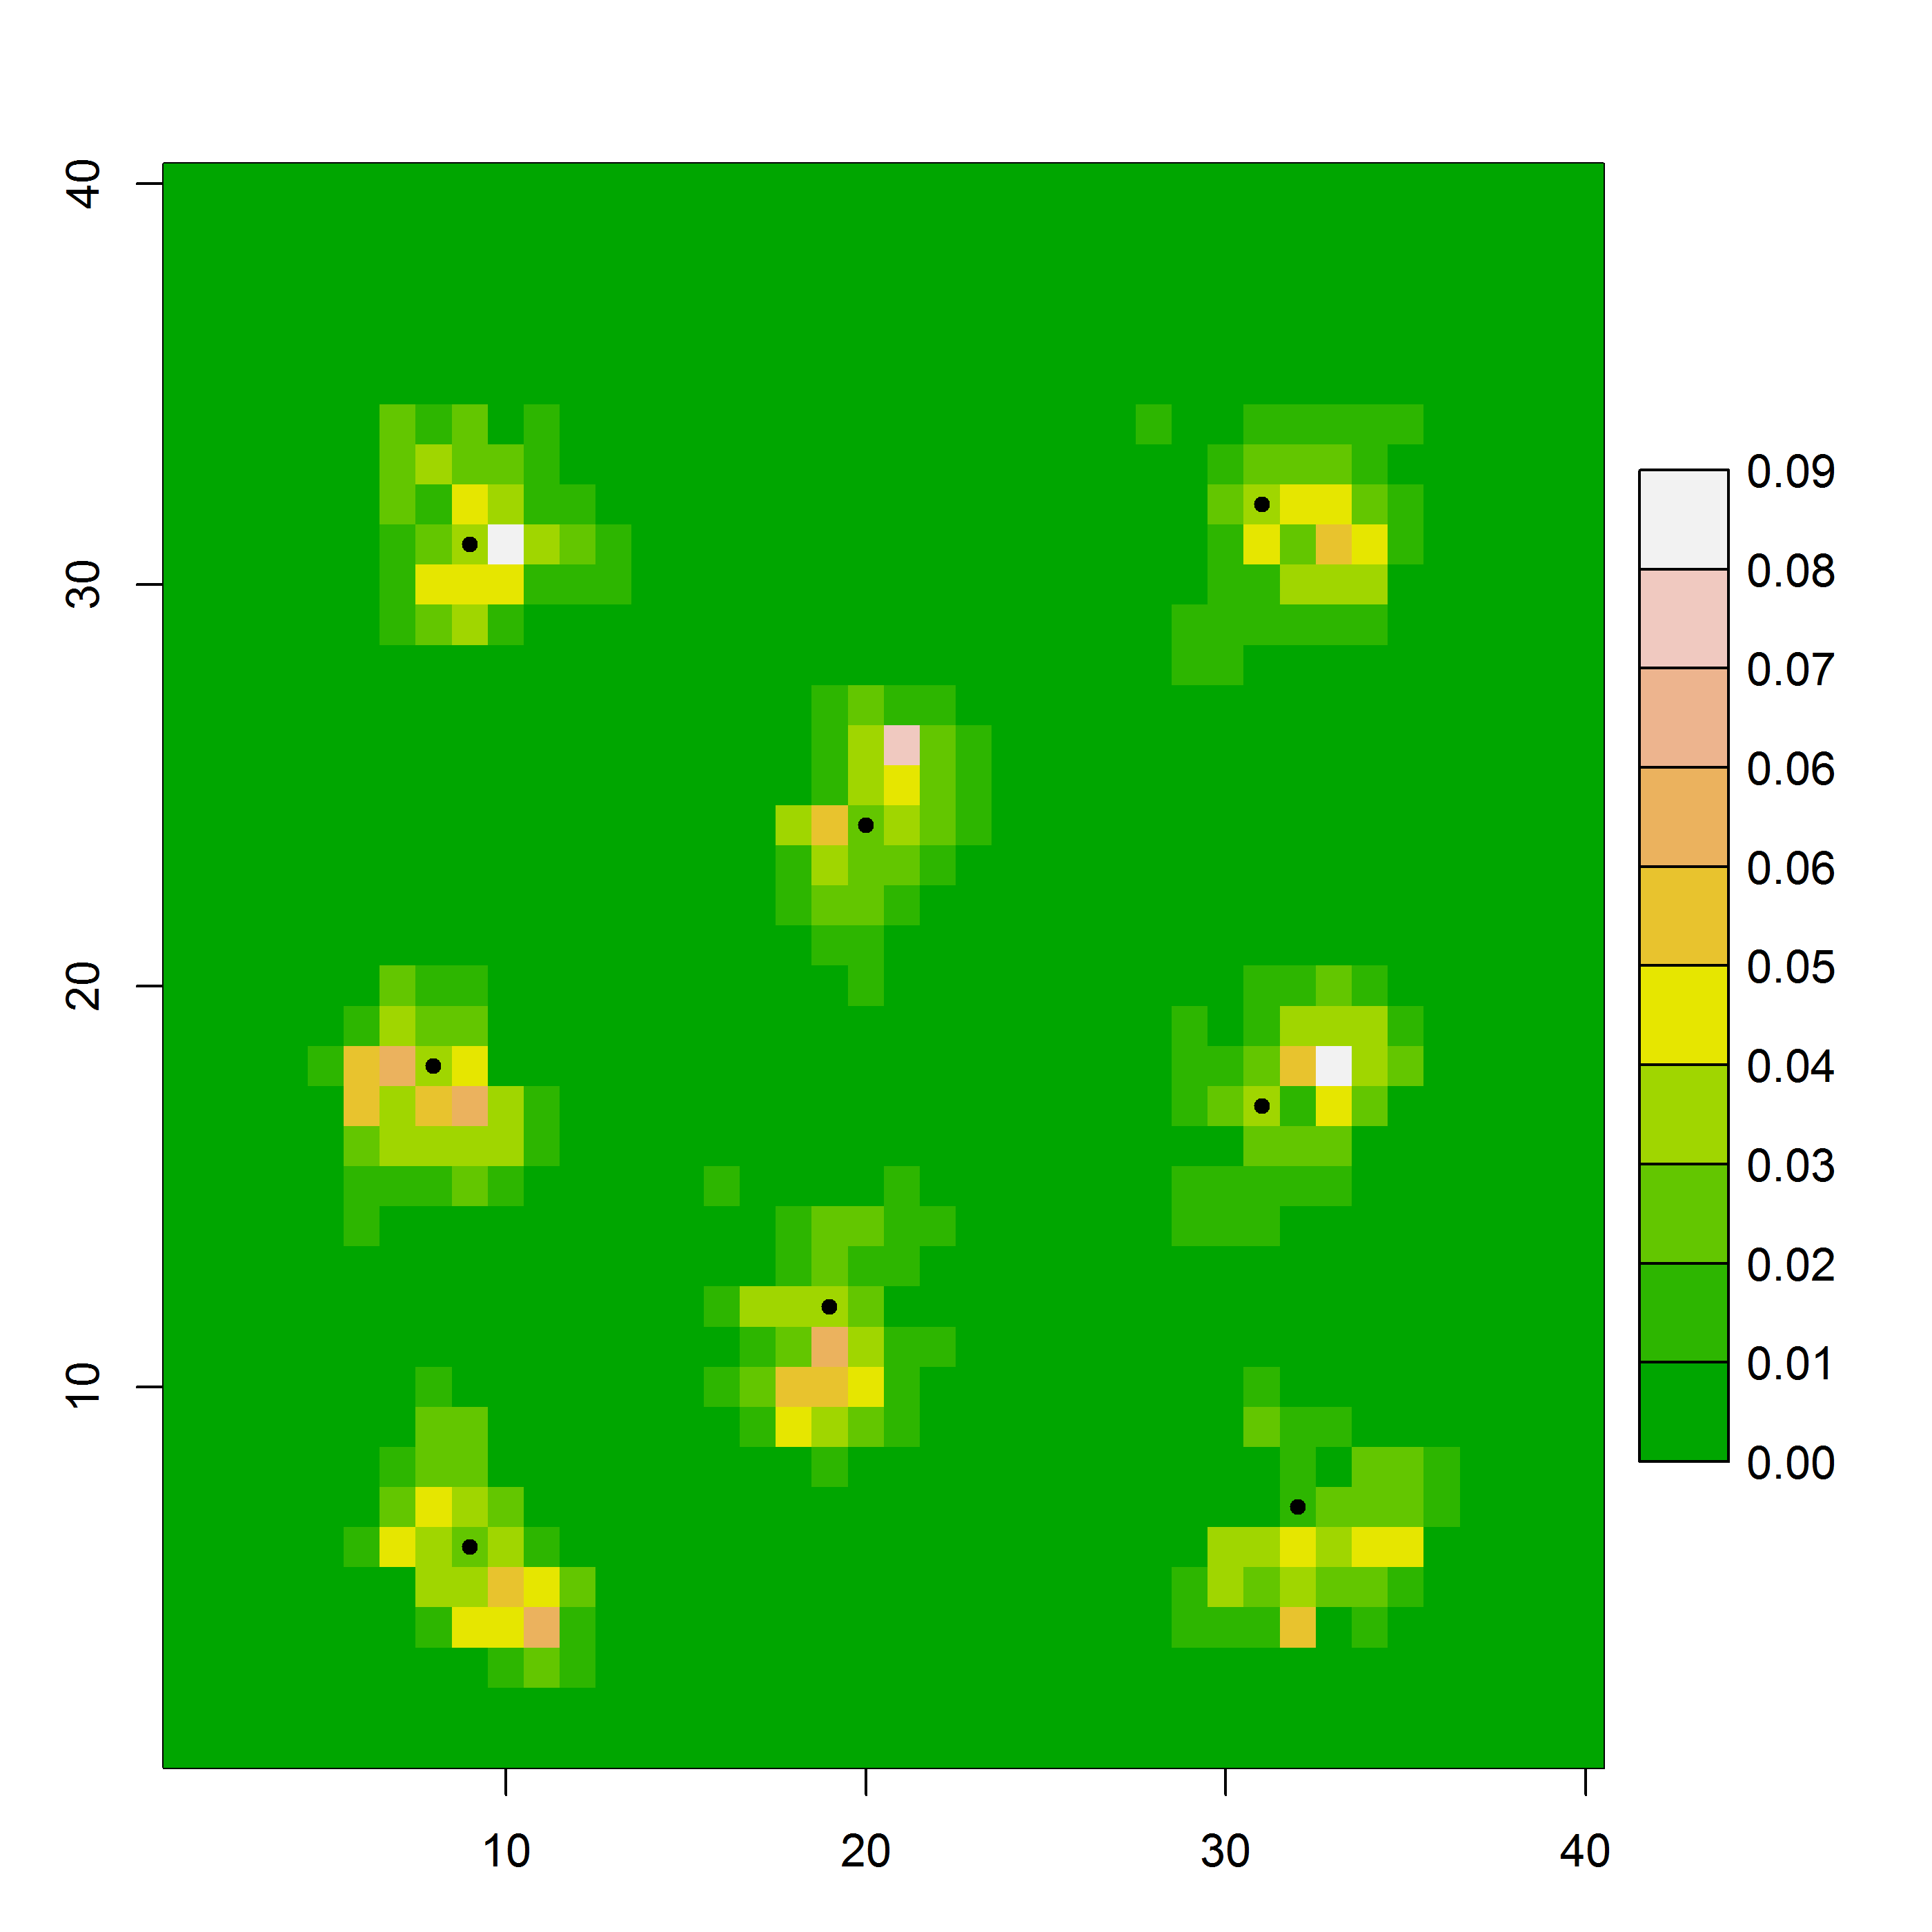
\includegraphics[width=3.5in,height=3.5in]{Ch13-RSF/figs/homeranges8}
\caption{Space usage patterns of 8 individuals under a space usage
  model that contains a single covariate which is shown in
  Fig. \ref{rsf.fig.habitat}. The plotted value is the multinomial
  probability $\pi_{ij}$ for pixel $j$ under the model in Eq. \ref{rsf.eq.rsf}.
}
\label{rsf.fig.homeranges}
\end{figure}
The covariate in this case was simulated using a kriging
model of correlated random noise
with the following {\bf R} commands:
\begin{verbatim}
> set.seed(1234)
> gr <- expand.grid(1:40,1:40)
> Dmat<-as.matrix(dist(gr))
> V <- exp(-Dmat/5)
> C <- t(chol(V))%*%rnorm(1600)
\end{verbatim}
The resulting covariate vector ${\bf C}$ is multi-variate normal with
mean 0 and variance-covariate matrix ${\bf V}$ which, here, has
pariwise correlations which decay exponentially with distance. 
Home ranges shown in Fig.~\ref{rsf.fig.homeranges} were simulated
with $\alpha_{1} =
1/(2\sigma^2)$, with $\sigma = 2$, and the coefficient on $C({\bf x})$
set to $\alpha_{2} = 1$. The resulting space usage densities -- ``home ranges'' -- exhibit clear
non-stationarity in response to the structure of the underlying
covariate, and they are distinctly asymmetrical.  We note that if
$\alpha_{2}$ were set to 0, the 8 home ranges shown here would
be proportional to bivariate normal kernels with $\sigma = 2$.
The commands for the kringing model, and those to produce Fig. \ref{rsf.fig.habitat} are in
the package \mbox{\tt scrbook} (see \mbox{\tt ?RSF$\_$example}).
\begin{figure}[ht]
\centering
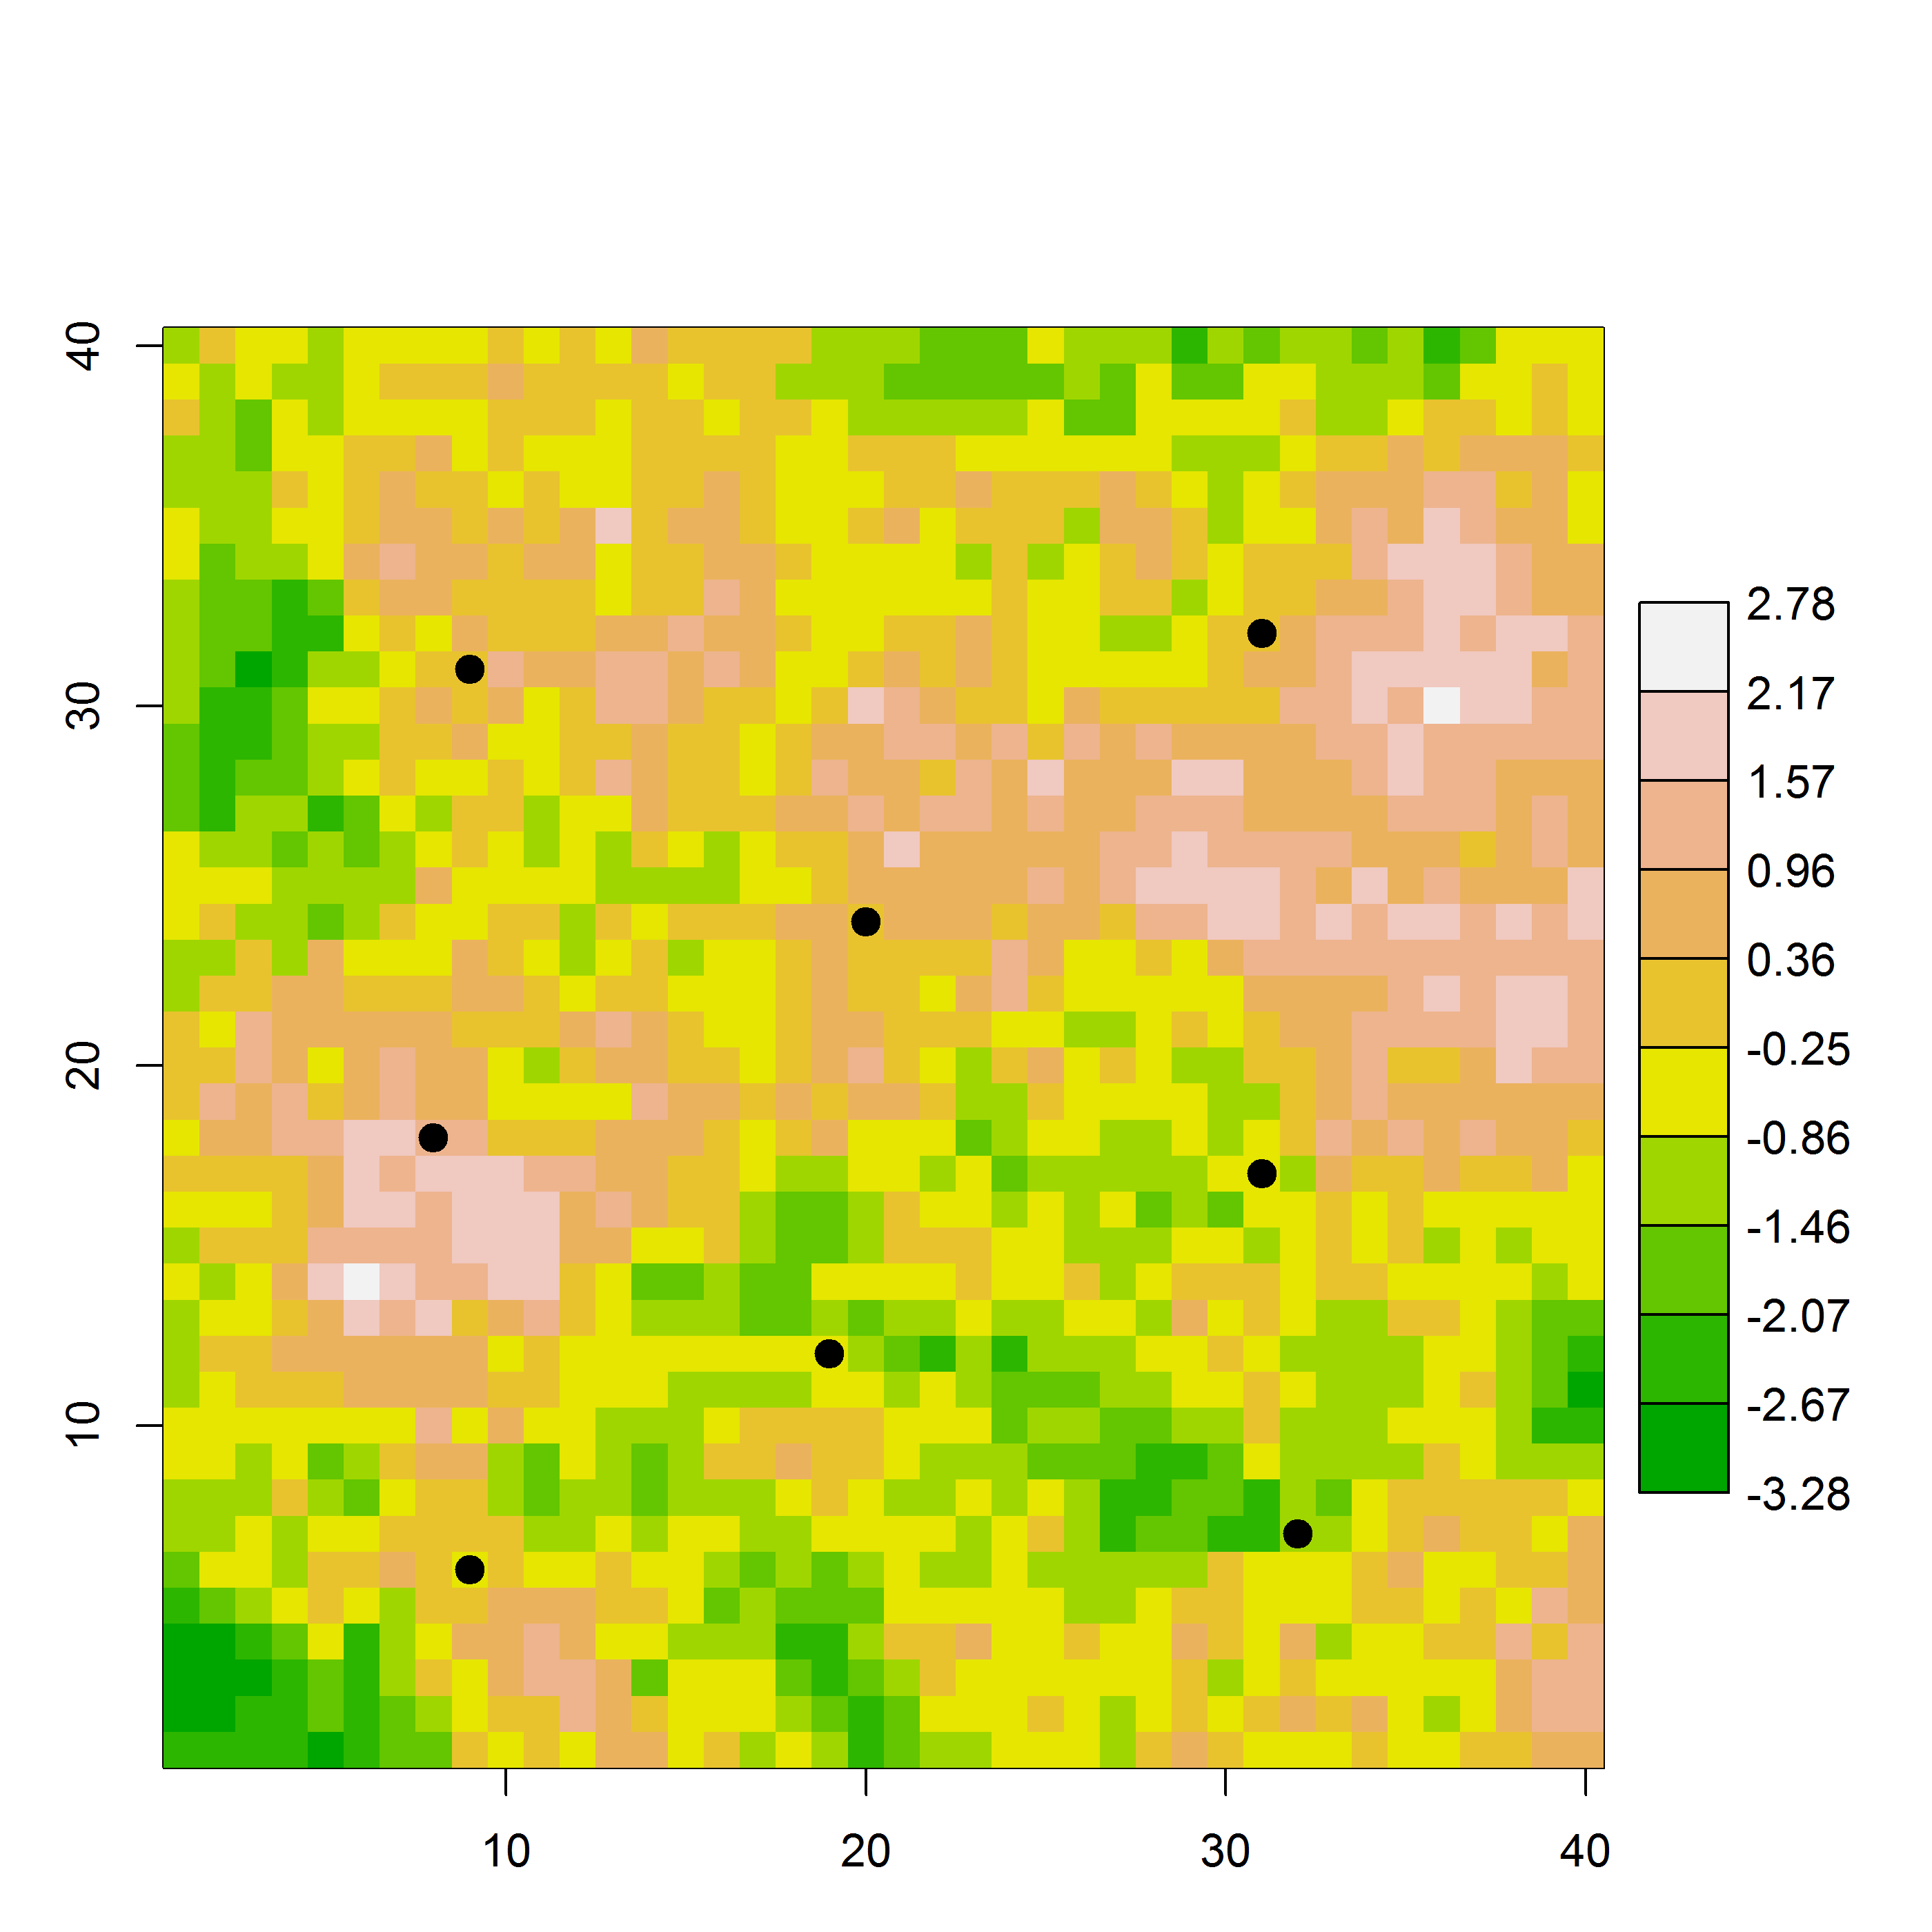
\includegraphics[width=3.15in,height=2.93in]{Ch13-RSF/figs/habitat.png}
\caption{A typical habitat covariate reflecting habitat quality or
  hypothetical utility of the landscape to a species under study. Home
  range centers for 8 individuals are shown with black dots.}
\label{rsf.fig.habitat}
\end{figure}
%XXX RS: I think I'd bring the habitat figure first, then the home ranges XXXX

\subsection{Poisson model of space use}

A natural way to motivate the multinomial model of space usage is to
assume that individuals make a sequence of resource selection
decisions so that the outcomes $m_{ij}$ are {\it
  independent} Poisson random variables:
\[
 m_{ij} \sim \mbox{Poisson}( \lambda_{ij})
\]
where
\[
 \log(\lambda_{ij}) = a_{0} -\alpha_{1} d_{ij}^{2} +  \alpha_{2} C({\bf x}_{j})
\]
In this case, the number of visits to any particular cell is affected
by the covariate $C({\bf x})$ but has a baseline rate, $\exp(a_{0})$,
related to the amount (in an expected value sense) of movement occuring over some time interval.
This is an equivalent model to the multinomial model given previously
in the sense that, if we condition on the total sample size $R = 
\sum_{j} m_{ij}$, then the vector ${\bf m}_{i}$ has a multinomial
distribution with probabilities given by Eq. \ref{rsf.eq.rsf} (see
also Chapt. \ref{chapt.poisson-mn}).  Also note that if use
frequencies are summarized over individuals for each pixel, i.e.,
create the totals $m_{.j} = \sum_i m_{ij}$, then a standard Poisson
regression model for the resulting ``quadrat counts'' is
reasonable. This is ``Design I'' in \citet{manly_etal:2002}.
%XXX maybe say what design I relates to - is it RSF specific or something else?
%%% Richard: can you embellish this a little bit?
% XX RS: Agree: Needs one or two sentences on design 1; also, before you cite Johnson and his levels of selection, then Manly's protocoll A, now design 1. Would be nice to reconcile all those. Maybe a table with the definitions? It just gets messy with 3 different scales/structures for the same problem XXXX

In practice, we never observe ``truth'', i.e., the actual use
frequencies $m_{ij}$. Instead, we observe a sampling XXX sample? XXX of the actual use
outcomes by an individual.  As formulated in
Sec.~\ref{scr0.sec.implied}, we assume a binomial (``random'')
sampling model:
\[
 y_{ij} \sim \mbox{Binomial}(m_{ij}, p_{0}).
\]
We can think of these counts as arising by thinning the underlying
point process (here, aggregated into pixels) where $p_{0}$ is the
thinning rate of the point process.  
% XXX RS: So far we've used point process to describe distribution of s in S. But now you mean the telemetry locations, right? Would make that more explicit XXXXX
In this case, the marginal
distribution of the observed counts $y_{ij}$ is also Poisson but with mean
\[
 \log(\mathbb{E}(y_{ij}))  = \log(p_{0}) + a_{0} -\alpha_{1} d_{ij}^{2} +  \alpha_{2} C({\bf x}_{j}).
\]
Thus, the space-usage model (RSF) for the thinned counts $y_{ij}$ is
the same as the space-usage model for the original variables $m_{ij}$.
This is because if we remove $m_{ij}$ from the conditional model by
summing over its possible values, then the vector ${\bf y}_{i}$ is
{\it also} multinomial with cell probabilities
\[
\pi_{ij} = \frac{\lambda_{ij}}{\sum_{j} \lambda_{ij}}
\]
where any constant (the intercept term $a_0$ and thinning rate
$p_{0}$)
cancel 
from the numerator and denominator. Thus, the underlying multinomial
RSF model applies to the true unobserved count frequencies ${\bf
  m}_{i}$ and also those produced from thinning or sampling, ${\bf
  y}_{i}$.


\section{Integrating Capture-Recapture Data}

The key to combing RSF data with SCR data is 
to note that the Poisson model of space usage given above is 
exactly our Poisson encounter probability model from
Chapt. \ref{chapt.poisson-mn}, but with some arbitrary intercept off-set
related to the 
sampling rate by the telemetry device, and with
a spatial covariate  $C({\bf x})$.
We've used exactly this model for our SCR data (Chapt. \ref{chapt.covariates}), but with a different intercept,
$\alpha_{0}$, unrelated to the intercept of the Poisson use model
for telemetry described above but, rather, to the efficiency of the capture-recapture
encounter device. 
In other words, we view camera traps (or other devices) located in
some pixel ${\bf x}$ (or multiple pixels) as being equivalent to being able to turn on a
type of (less perfect) telemetry device only in that pixel.
%result of some thinning of the ``true'' space usage outcomes.
%In other words, imagine that we have a sampling device, such as a
%camera trap, in {\it every} pixel. If the device operates continually
%then it functions similar to a telemetry instrument in the sense that
%we can observe an individual in {\it any} pixel. But, given that 
%Given that real sampling devices
% operate imperfectly, intermittently, or do not expose the
%entire area of each pixel, then a reasonable model for this imperfect
%observation is the ``thinned'' binomial model given above, but with a
%different 
%intercept, say 
%representing the sampling
%effectiveness of the device, what we've called the baseline encounter
%rate in previous chapters. 
Therefore, 
data from a camera trapping are Poisson random variables 
for every pixel $j$ where a trap is located:
\[
y_{ij}|{\bf s}_{i} \sim \mbox{Poisson}( \lambda_{ij})
\]
with 
\[
 \log(\lambda_{ij}) =  \alpha_{0} -\alpha_{1}
 d_{ij}^{2} +  \alpha_{2} C({\bf x}_{j}).
\]
The parameters $\alpha_{1}$ and $\alpha_{2}$ are shared with the
multinomial model for the telemetry data.

Alternatively, 
the SCR study can produce binary 
encounters depending on the type of sampling being done,
where $y_{ij} = 1$ if the individual $i$ visited
the pixel containing a trap and was detected, then we imagine that
$y_{ij}$ is related to the latent variable $m_{ij}$ being the event
$m_{ij}>0$, which occurs with probability
\begin{equation}
 p_{ij} = 1-\exp(- \lambda_{ij})
\label{rsf.eq.cloglog}
\end{equation}
%We combine the constants so that $\alpha_{0} = \log(\lambda_{0}) + a_{0}$
%is the baseline encounter rate which includes the constant intensity
%of use by the individual and also the baseline rate of detection,
%conditional on use.  The Bernoulli observation model implies that the
and then the observed encounter frequencies for individual $i$ and trap $j$, from
sampling over $K$ occassions are binomial:
\[
 y_{ij}|{\bf s}_{i} \sim \mbox{Binomial}(K, p_{ij}) 
\]

A key point here is that if resource selection is happening, then it
appears as a covariate on encounter rate (or encounter
probability) in the same way as ordinary covariates which were discussed in
Chapt. \ref{chapt.covariates}.


\subsection{The Joint RSF/SCR Likelihood}

To construct the likelihood for SCR data when we have 
direct information on space usage
from telemetry data, we regard the two samples (SCR and RSF) as
independent of one another, and we 
 form the likelihood for each set of observations as a function
of the same underlying parameters. The joint likelihood then is the
product of the two components. 

In particular, let ${\cal L}_{scr}(\alpha_{0}, \alpha_{1}, \alpha_{2}, N;{\bf y})$
be the likelihood for the SCR data in terms of the basic encounter
probability parameters and the total (unknown) population size $N$,
and let ${\cal L}_{rsf}(\alpha_{1},\alpha_{2}; {\bf m})$ be the
likelihood for the RSF data based on telemetry which, because the
sample size of telemetered individuals is fixed, does not depend on $N$.
Assuming independence of the two datasets, the
joint likelihood is the product of these two pieces:
\[
{\cal L}_{rsf+scr}(\alpha_{0},\alpha_{1},\alpha_{2},N; {\bf y},{\bf
  m})  =
{\cal L}_{scr}(\alpha_{0}, \alpha_{1}, \alpha_{2}, N;{\bf y})
\times
{\cal L}_{rsf}(\alpha_{1},\alpha_{2}; {\bf m}),
\]
where the ${\cal L}_{scr}$ is the standard integrated likelihood
(Chapt. \ref{chapt.mle}), and the RSF likelihood contribution is the
multinomial telemetry likelihood having cell probabilities
Eq. \ref{rsf.eq.rsf}.  The {\bf R} code for this 
%XXX to maximize the joint likelihood? or for what? XXX 
was given in the
supplement to \citet{royle_etal:2012mee}, and we include a version of
this in the \mbox{\tt scrbook} package, see \mbox{\tt ?intlik3rsf},
which also shows how to simulate data and fit the combined SCR+RSF
model.

%XXX a lot of our book is from papers, but this section below sounds
%particularly like we didn't try.  I revised it a bit, hope you think it's okay
%% Andy sez: Beth -- thanks for that, I think this is good. I might
%% micro-edit it.

\section{SW  New York Black Bear Study}
\label{rsf.chapt.nybears}

\citet{royle_etal:2012mee} applied the integrated SCR+RSF model to
data from a study of black bears ({\it Ursus americanus})
in a region of approximately 4,600
km$^2$ in southwestern New York \citep{sun:2013}\footnote{This is
different from our Fort Drum bear study data set which we've analyzed
in previous chapters}.  The data can be loaded from the \mbox{\tt scrbook}
library with the command \mbox{\tt data(nybears)}.
We reproduce the findings of \citet{royle_etal:2012mee} in this section.

The data are based on a noninvasive genetic capture-recapture study
using 103 hair snares in June and July, 2011.  Hair snares were baited
and scented and checked weekly for hair \citep{sun:2013}.  The study
yielded relatively sparse encounter histories
 of 33 individuals with a total of 14 recaptures (27
individuals captured 1 time only.
% Extra trap recaptures included  %XXX what is an extra trap recap?
%3 individuals captured in 2 traps, 1 individual in each of 3 and 4
%traps).  
Telemetry data were collected on 3 telemetry-collared individuals, which produced
locations for each bear approximately once per hour.  We 
thinned these data to once per 10 hours to produce movement outcomes that might
be more independent. This produced 195 telemetry locations used in the
RSF component of the model.  Elevation was used as the covariate for this 
model, a standardized version of which is shown in
Fig. \ref{fig.elevation} along with the locations of each
capture at hair snare sites.  


\begin{figure}[ht]
\centering
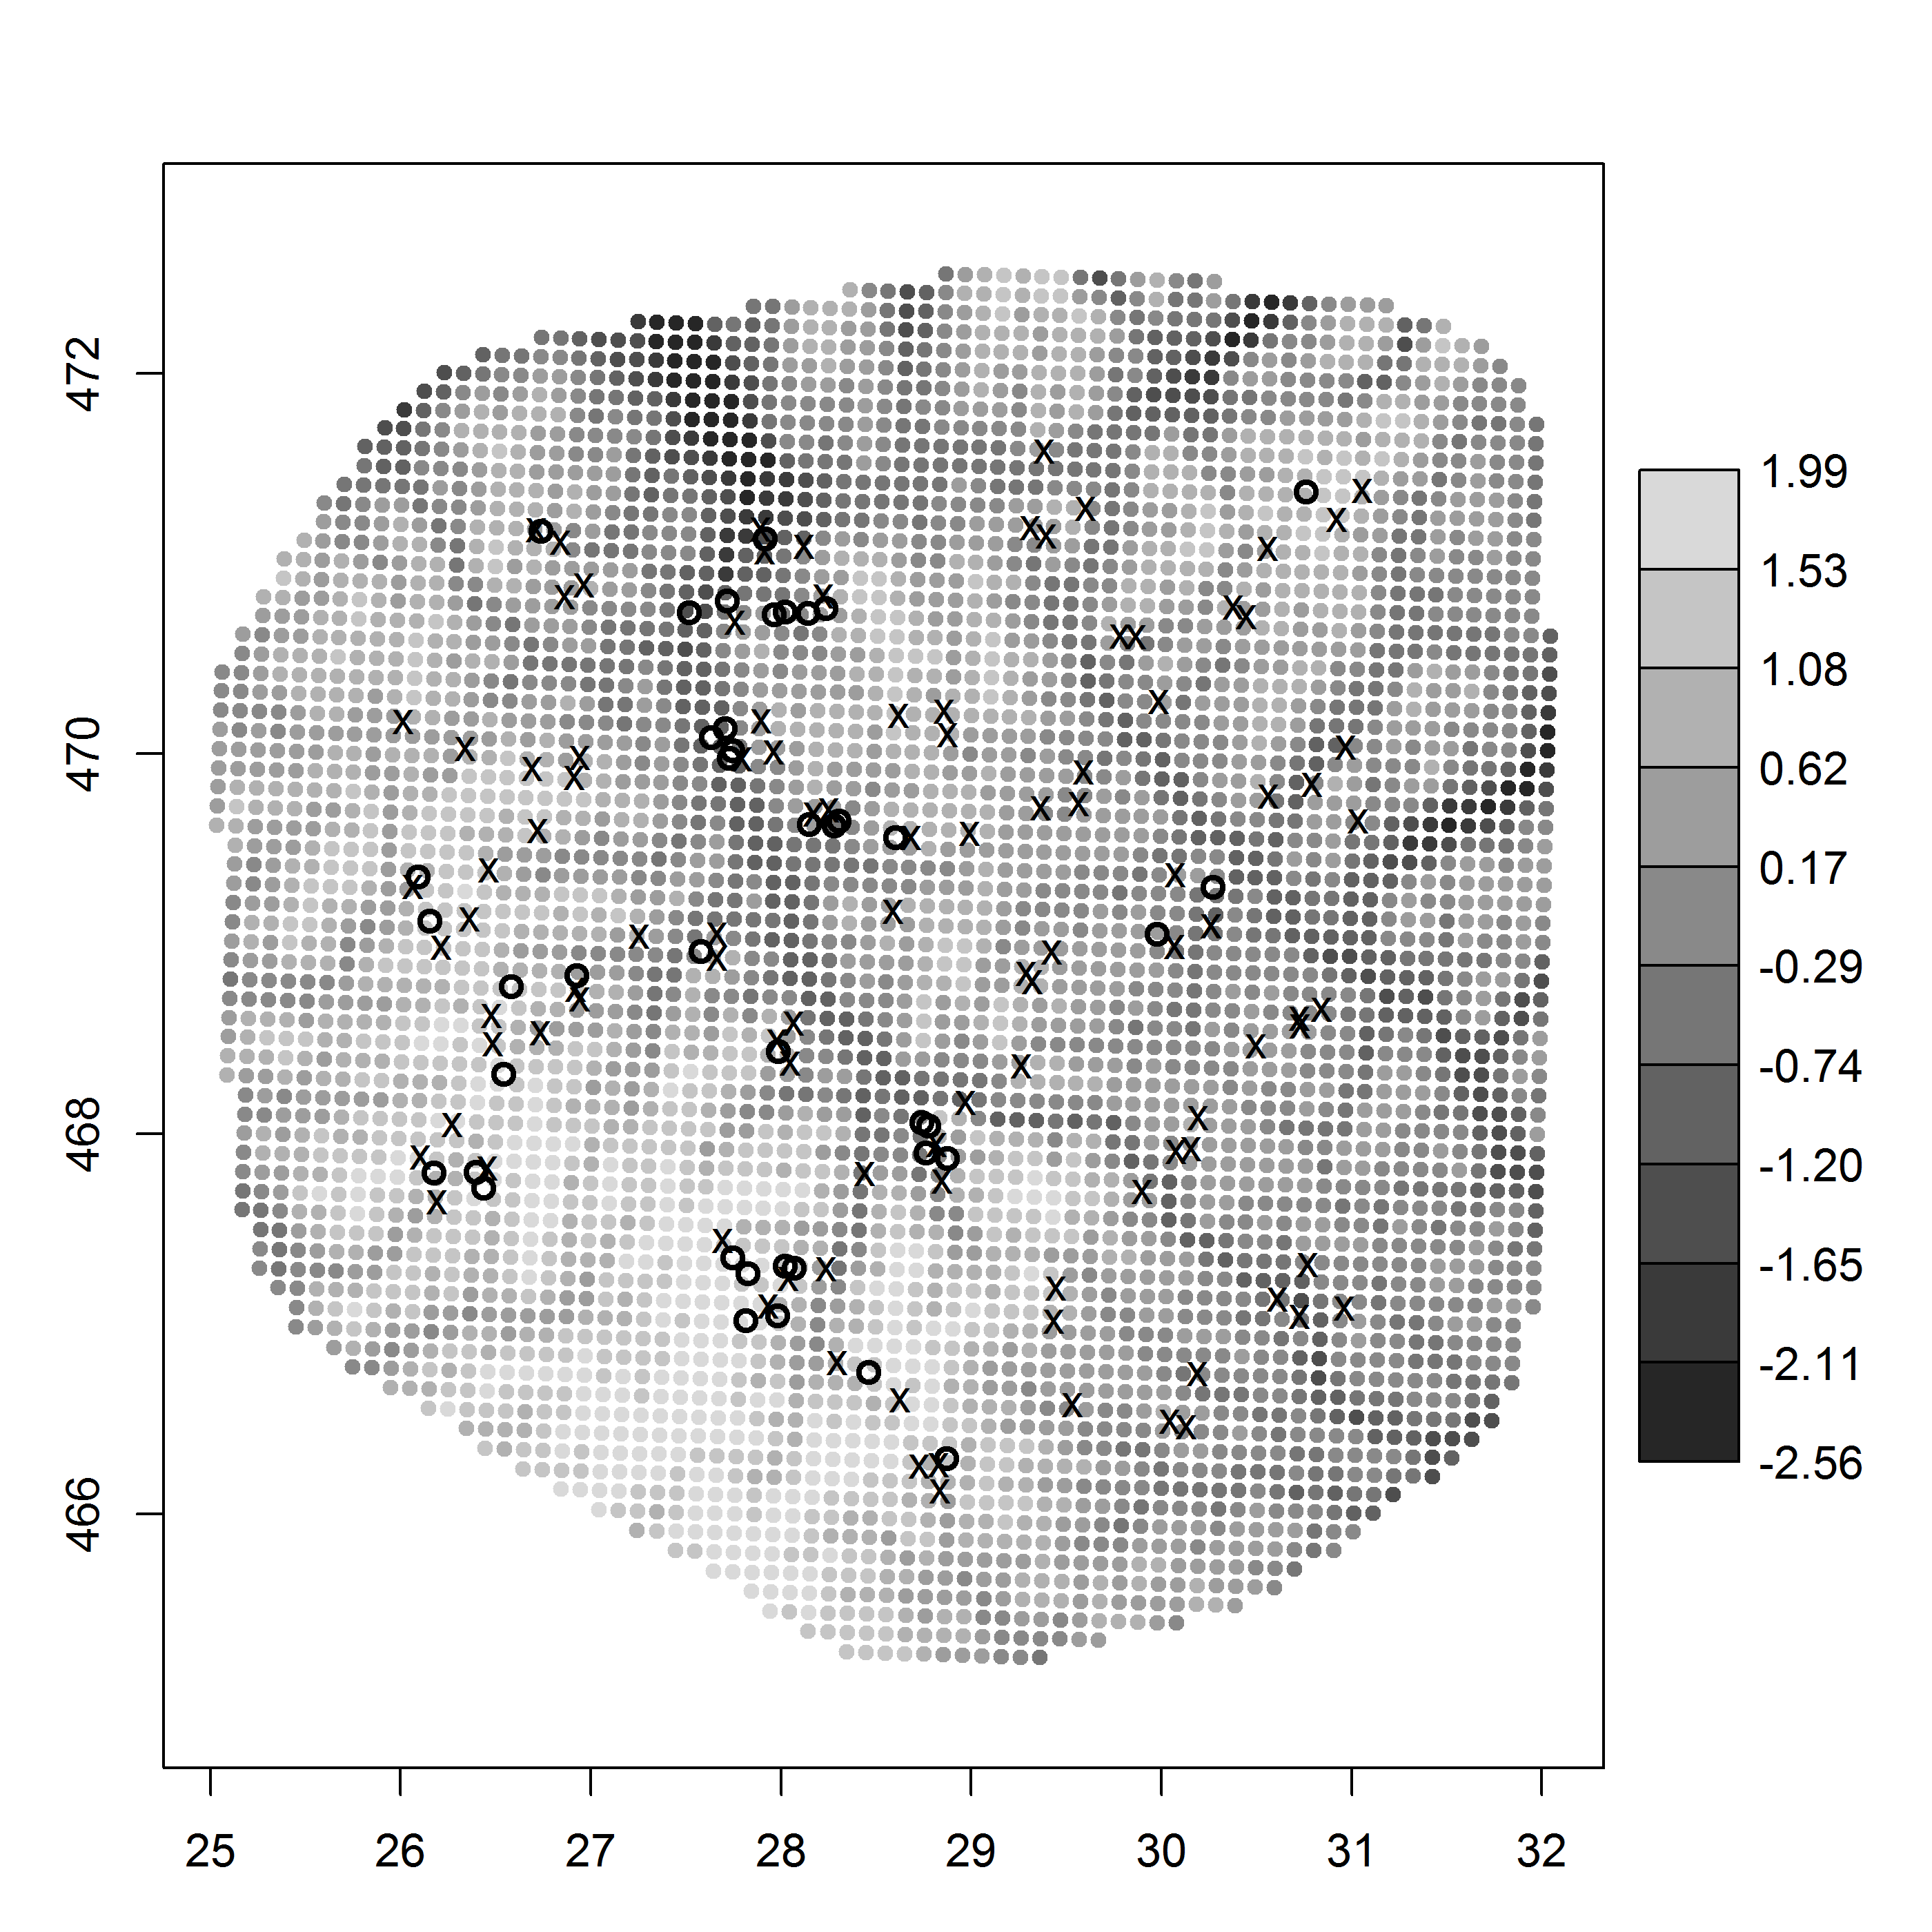
\includegraphics[width=3.25in,height=3.25in]{Ch13-RSF/figs/elev_captures_bw.png}
\caption{
Elevation (standardized), hair snare locations (indicated by ``$x$'') and location
of bear captures (open circles).
Multiple captures at a trap location are offset by adding
random noise.
}
\label{fig.elevation}
\end{figure}

%XXXX RS: I think this figure needs some work; symbols are difficult to distinguish. XXXX

There are a number of models that could be fitted to these data based on
the combination of SCR and RSF data as well as the elevation covariate.  
The models fit here are
 based on the Gaussian hazard trap encounter/space usage model,
including an ordinary SCR model with no covariates or telemetry data,
the SCR model with elevation affecting either $\lambda_{0}$ or density
$D({\bf x})$ (Chapt. \ref{chapt.state-space}), and models that use
telemetry data.  The 6 models fitted were:
\begin{itemize}
\item[] Model 1,  SCR: ordinary SCR model
\item[] Model 2, SCR+p(C): ordinary SCR model with elevation as a
  covariate on baseline encounter probability $\lambda_{0}$.
\item[] Model 3, SCR+D(C): ordinary SCR model with elevation as a
  covariate on density only.
\item[] Model 4, SCR+p(C)+D(C): ordinary SCR model with elevation as
  a covariate on both baseline encounter probability and density.
\item[] Model 5, SCR+p(C)+RSF: SCR model including data from 3
  telemetered individuals.
\item[] Model 6, SCR+p(C)+RSF+D(C): SCR model including telemetered
  individuals and with elevation as a covariate on density.
\end{itemize}
It is tempting to want to compare these different models by AIC but,
because models 5 and 6 involve additional data, they cannot be
compared with models 1-4.  Parameter estimates for the six models are
given in Table \ref{tab.nyresults} (reproduced from
\citet{royle_etal:2012mee}, see also the help file \mbox{\tt
  ?nybears}).

By looking at Table \ref{tab.nyresults}, it is clear based on the
negative log likelihood for just Models 1-4, that those containing an
elevation effect on density are preferred (Model 3 and 4).  The
parameter estimates indicate a positive effect of elevation on
density, which seems to be consistent with the raw capture data shown
in Fig. \ref{fig.elevation}.  Despite this strong effect
of elevation, the estimates of $N$ under each of these models only
ranged from $93 - 103$ bears for the 4600 km$^2$ state-space.
%XXX RS: So density is pretty constant across models? XXX
  If we
consider not just density, but space usage (i.e., looking at the
parameter $\alpha_2$), the effect of elevation is negative.  Thus, elevation, appears to affect density and space usage
differently.  It was suggested that density operates at the
second-order scale of resource selection and ``....is largely related
to the spacing of individuals and their associated home ranges across
the landscape.  On the other hand, our RSF was defined based on
selection of resources within the home range (third-order).''
\citep{royle_etal:2012mee} 
%XXXX RS: Since you bring up second-order resource selection here, the different orders def. need to be defined earlier on XXX
The positive effect of density on elevation
is consistent with some other studies XXX on black bears? XXXX \citep[e.g.][]{frary_etal:2011},
and the negative effect of elevation on space usage can be attributed to
seasonal variation in food availability, usage of corridors, or
environmental conditions.


Models 5 and 6 include the additional telemetry data, thus the
negative log-likelihoods are not directly comparable to the first 4
models, but we can still make a few important observations.  First is
that the parameter estimates under these two models are consistent
with Model 4 in that elevation had a strong effect on both density and
space usage.  In comparing models 5 and 6, the latter model which
includes elevation as an effect on density reduces the negative
log-likelihood by 5 units.  Additionally, including the telemetry data
reduces the standard errors (SE) of the density and space usage
parameters and as we would expect, the incorporation of telemetry data
also reduces the SE for $\sigma$.  The increased precision for the
estimated population size ($N$) is negligible with the use of
telemetry data in this case.  However, that may be different if more
telemetry information were available.  Model 6 (SCR+p(C)+RSF+D(C)),
was used to produce maps of density (Fig. \ref{fig.density}) and space
usage (Fig. \ref{fig.spaceusage}) showing the effect of elevation on
both components of the model.  The map of space usage shows the
relative probability of using a pixel ${\bf x}$ relative to one having
the mean elevation, given a constant distance to the individual's
activity center.
 %XXXX is that a correct interpretation of what you did?


\begin{comment}

XXX Beth: I rewrote all of this above  
XXX you can put it all back in and take my stuff out if you want

{\bf XXXXXXXX below is exactly plagarized from the paper XXXXXXXXXXXX}
Looking at  models 1-4, which do not use the telemetry observations,
models in which elevation effects density are preferred, and we see a
a large positive response to elevation, which is apparent in
consistent with the visual pattern apparent in
Fig. \ref{fig.elevation} (more captures at higher elevations).
Conversely,
there is a negative effect of elevation on
space usage (the parameter $\alpha_{2}$).
The estimate of $N$ for the 4600 km$^2$ state-space, based on the best
model is about 103 bears $(\exp(4.25)+33)$.
In the two models that include the additional telemetry data, a couple
points stand out: Clearly the elevation effect on density is
important, reducing the negative log-likelihood by 5 units. The effect
of elevation on density and space usage are roughly consistent with
Model 4 which did not use telemetry data. Furthermore, the standard
errors (SE) of those two parameter estimates are reduced considerably
when the model uses telemetry data, as is the SE for estimating
$\log(\sigma)$.  The SE for estimating $\log(n_{0})$ is only improved
incrementally compared to the models without telemetry data.  We used
the best model, \mbox{\tt SCR+p(C)+RSF+D(C)}, to produce a map of
density (Fig. \ref{fig.density}) which shows clearly the pattern
induced by elevation. We also produced a map
(Fig. \ref{fig.spaceusage}) to illustrate the effect of elevation on
space usage. This shows the relative probability of using a pixel
${\bf x}$ relative to one of mean elevation, and of the same distance
from an individual's activity center.
% remind people how to compute "the relative prob of using pixel x XXXX
%The cool thing about these models is we can make pretty
%multi-colored maps of things.  A map of density under the
%model is shown in fig. \ref{fig.density}.  A map of space usage in
%terms of the relative probability of using pixel $x$ relative to the
%average pixel is shown in Fig. \ref{fig.spaceusage}.

\end{comment}

\begin{comment}
I computed the MLE of N and the SE using a delta approximation as
follows: The MEE paper has log(n0) and the se of log(n0) which is not informative.
> logn0<-c(4.140,4.110,4.114,4.255,3.884,4.028)
> sev<- c(0.366,0.362,0.358,0.377,0.363, 0.366)
> exp(logn0)+33
[1]  95.80282  93.94672  94.19099 103.45682  81.61830  89.14850
> sev*exp(logn0)
[1] 22.98583 22.06271 21.90638 26.56222 17.64844 20.55035
\end{comment}

%XXX RS: Table seems to wide and seems to have a different format from rest of the book (vertical line, more horizontal lines ) XXX
\begin{table}
\centering
\caption{
Summary of model-fitting results for the black bear study. Parameter
estimates are for the intercept ($\alpha_{0}$), logarithm of $\sigma$,
the
scale parameter of the Gaussian hazard encounter model, 
 $\beta$ is the coefficient of elevation on density, and the total
 population size $N$ of the state-space. Standard errors
 rae in parentheses.
The SCR data are based on $n=33$ individuals, and the telemetry data
are based on 3 individuals. 
}
\begin{tabular}{c|rrrrrr}
\hline \hline
model         & $\alpha_0$ & $\log(\sigma)$ & $\alpha_{2}$ & $N$ & 
$\beta$       & -loglik                                                                         \\ \hline
SCR(elev)      & -2.860    & -1.117        & 0.175       & 95.8        &        & 122.738  \\
             &  (0.390)     & (0.139)       & (0.248)       & (22.99)        &        &           \\
SCR          & -2.729    & -1.122        & ---          & 93.9        &        & 122.990  \\
              & (0.345)     & (0.140)       &              & (22.06)        &        &           \\
SCR+D(elev)      & -2.715    & -1.133        & ---          & 94.2        & 1.247 & 118.007  \\
              & (0.353)     & (0.139)       &              & (21.90)    & (0.408) &           \\
SCR(elev)+D(elev) & -2.484    & -1.157        & -0.384      & 103.5        & 1.571 & 117.075  \\
              & (0.391)     & (0.142)       & (0.276)       & (26.56)   & (0.463) &           \\
SCR(elev)+RSF       & -3.068    & -0.814        & -0.281      & 81.6        &        & 1271.739 \\
              & (0.272)    & (0.036)         & (0.118)       & (17.65)        &        &           \\
SCR(elev)+RSF+D(elev)  & -3.070    & -0.810        & -0.371      & 89.1        & 1.273 & 1266.700 \\
              & (0.272)    & (0.037)         & (0.124)       & (20.55)        & (0.411) &           \\
\hline
\end{tabular}
\label{tab.nyresults}
\end{table}



\begin{figure}
\centering
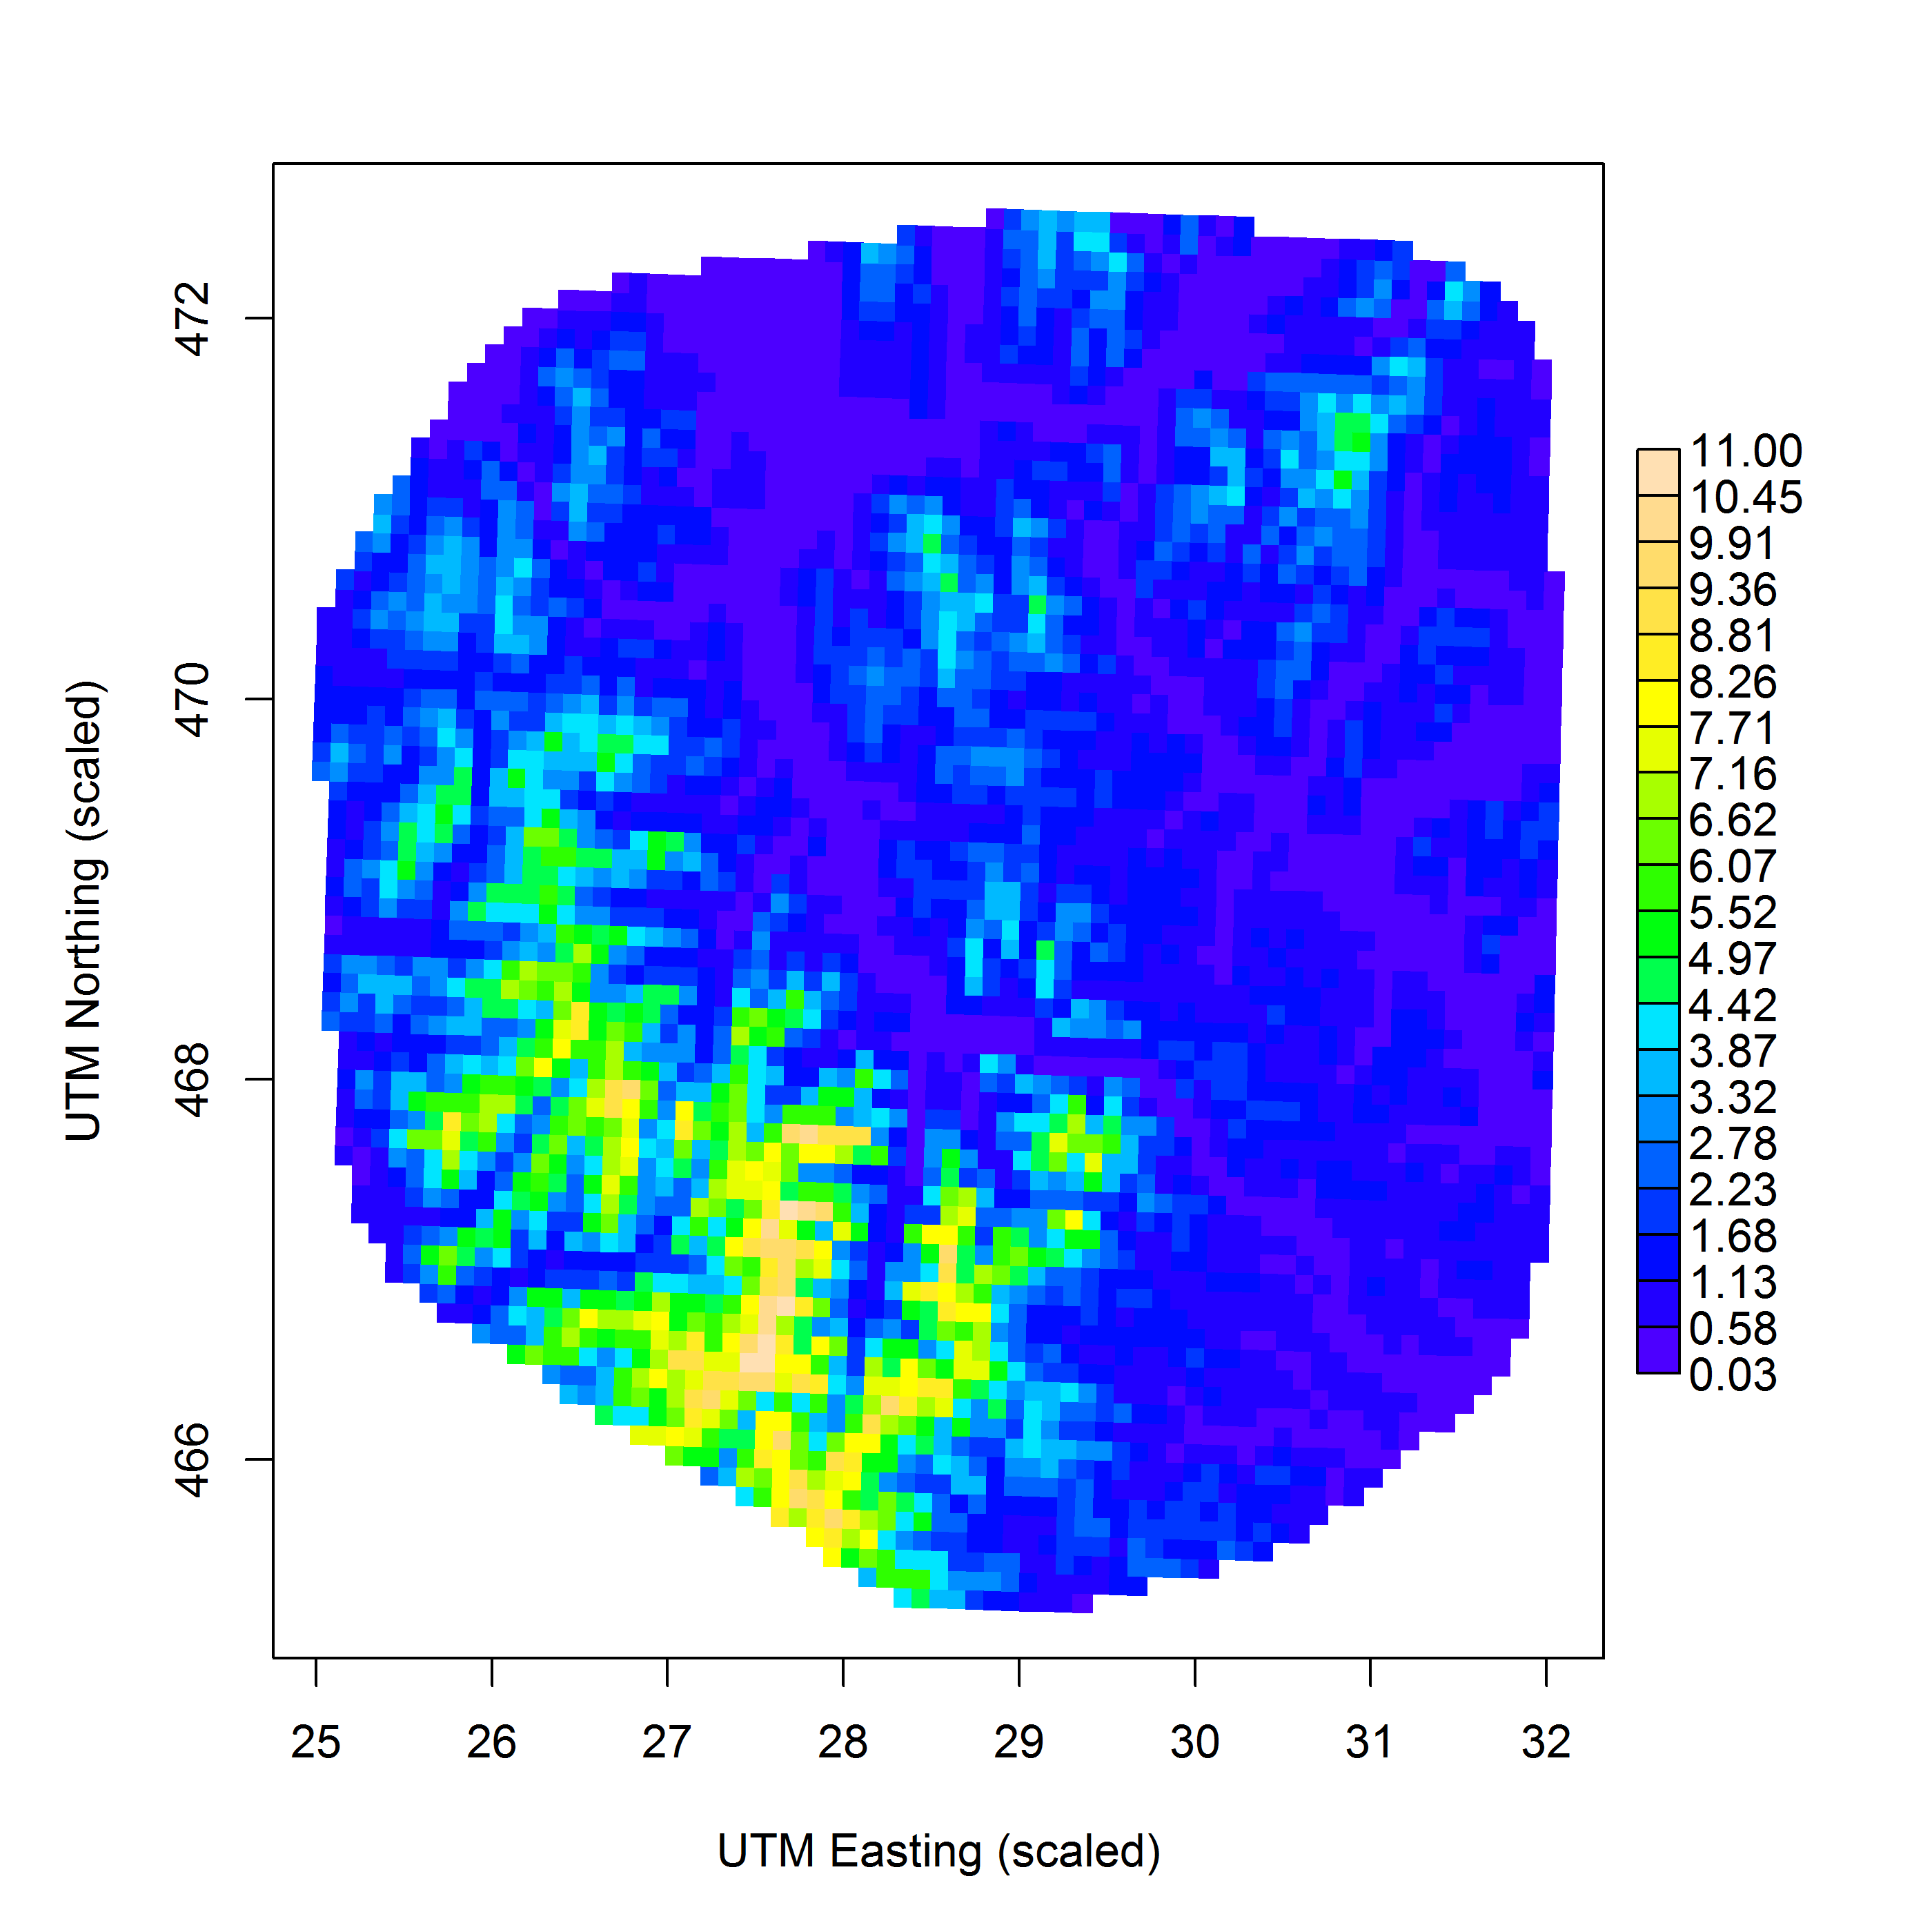
\includegraphics[width=3.25in,height=3.25in]{Ch13-RSF/figs/density2.png}
\caption{Predicted density of black bears (per 100 km$^2$) in
  southwestern  New York study
  area.
}
\label{fig.density}
\end{figure}


\begin{figure}
\centering
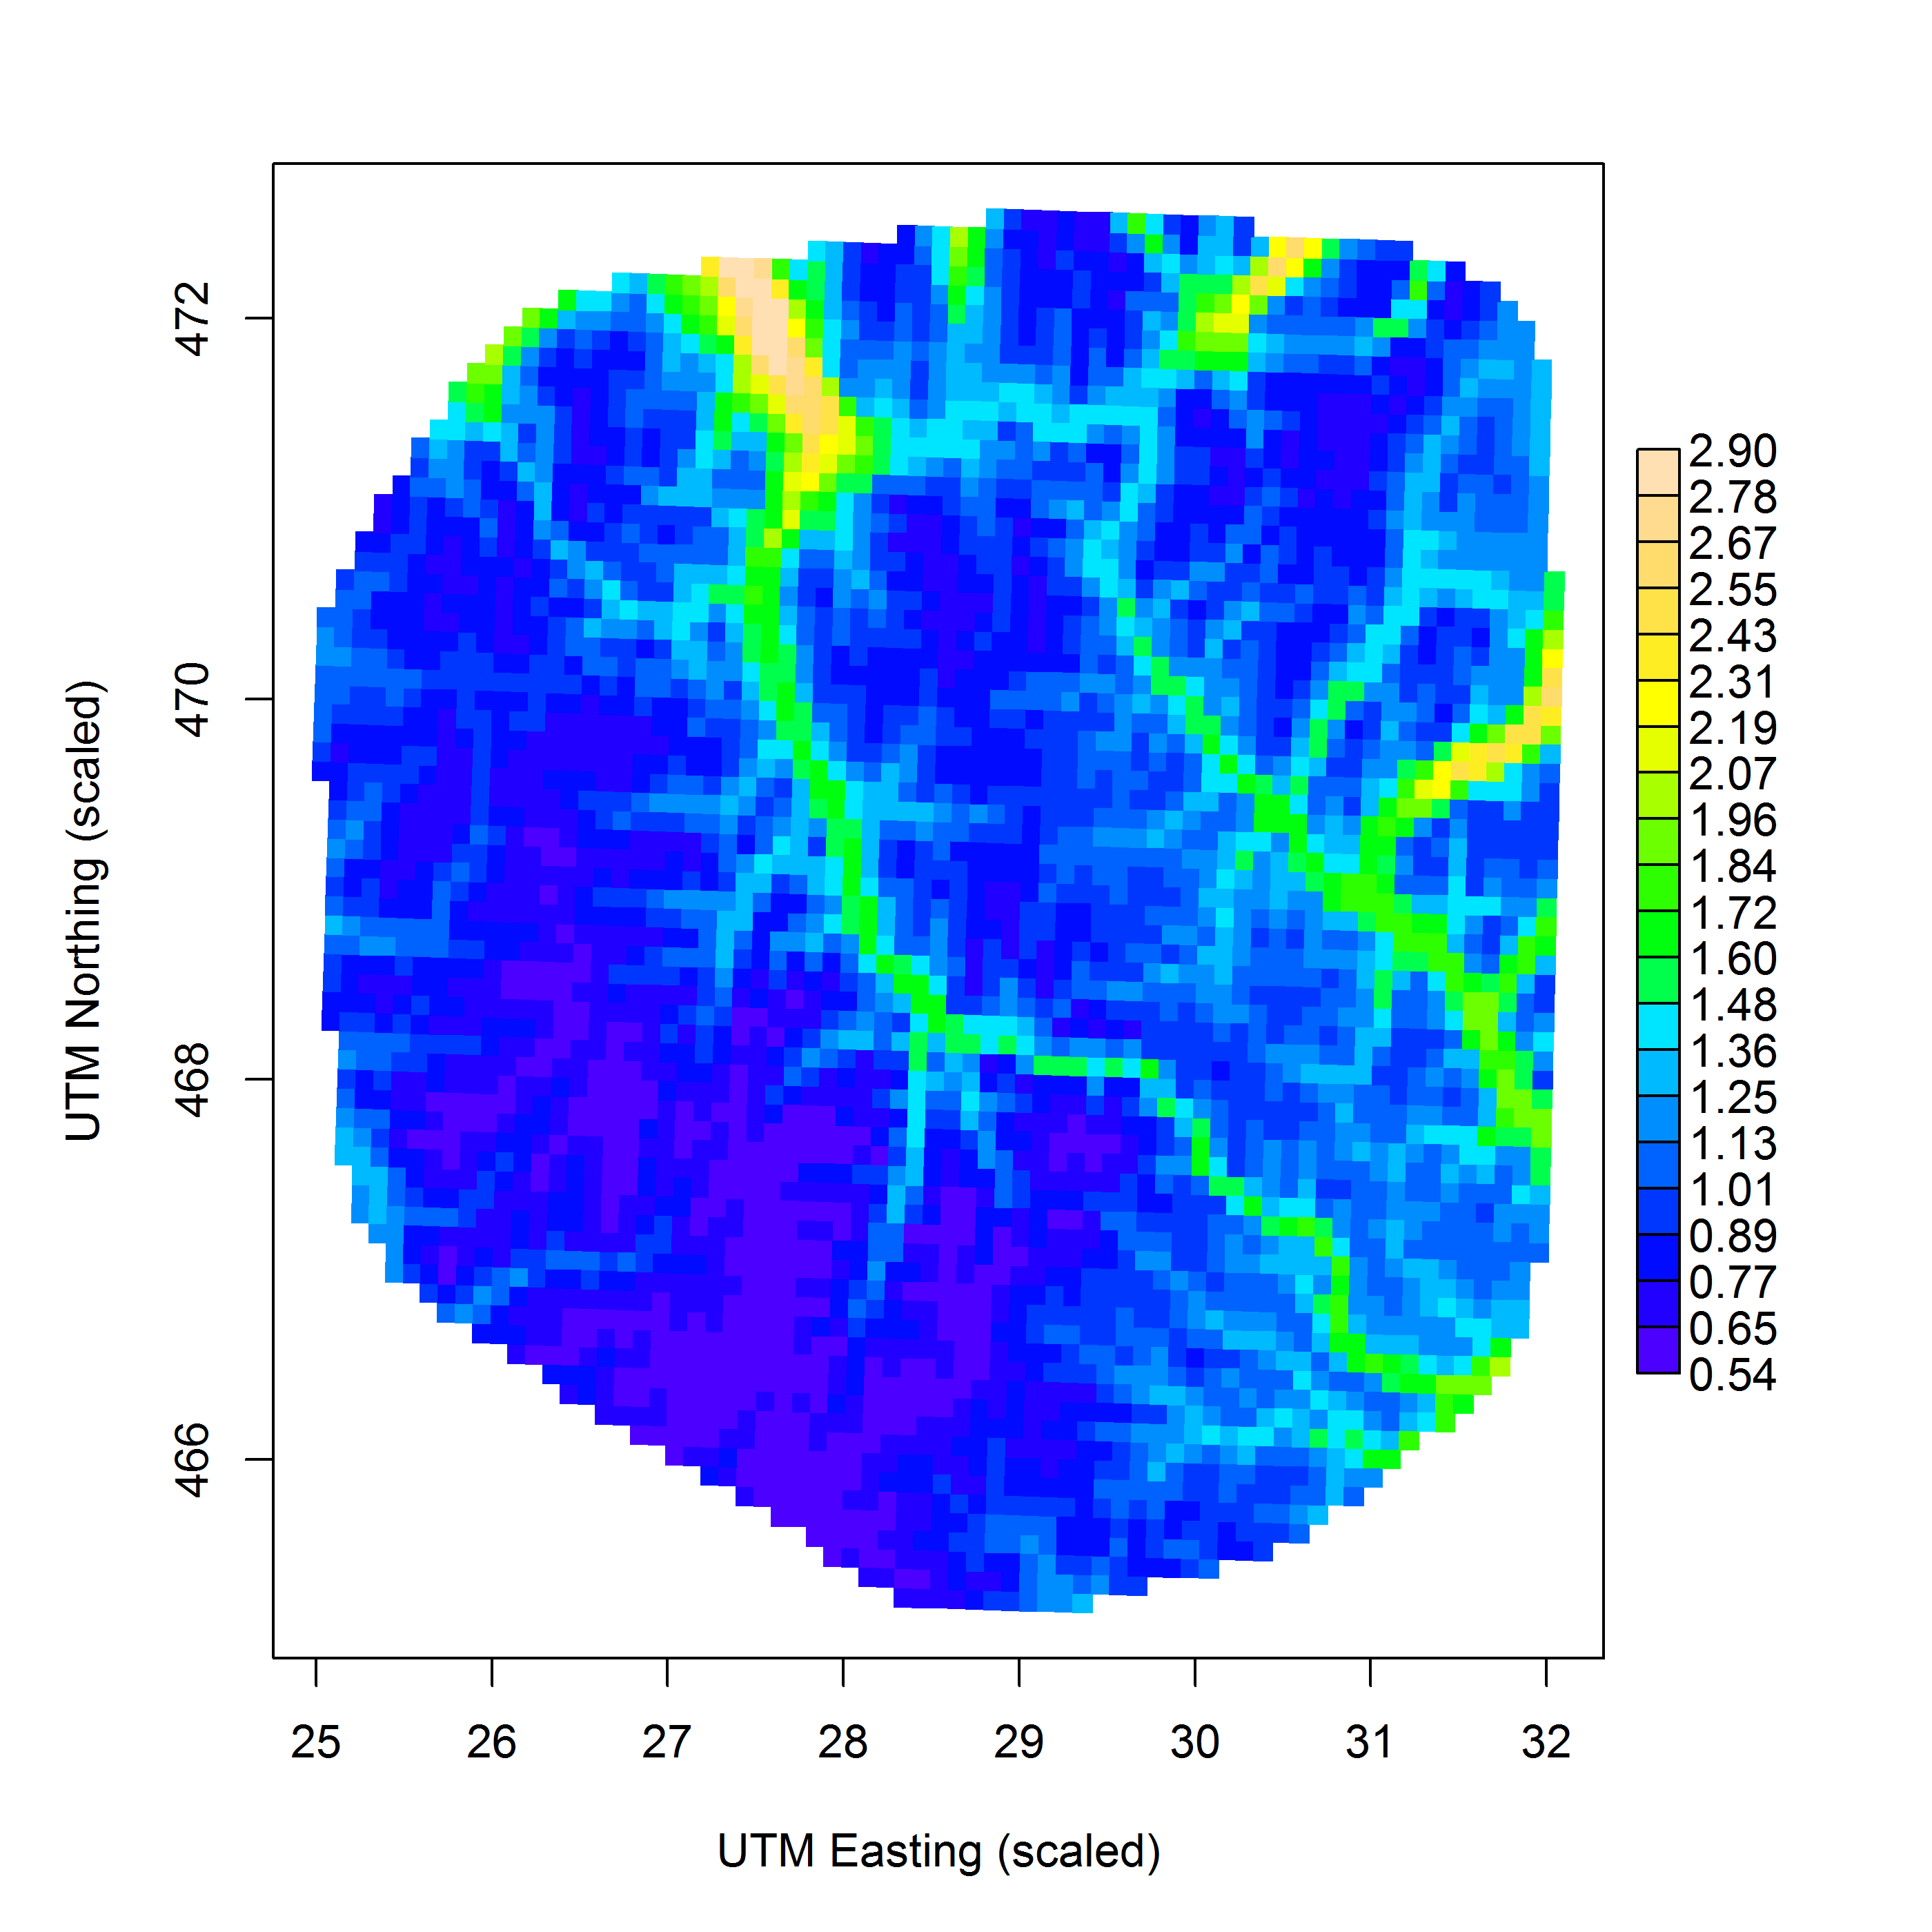
\includegraphics[width=3.25in,height=3.25in]{Ch13-RSF/figs/spaceusage2.png}
\caption{Relative probability of use of pixel ${\bf x}$ compared to a pixel
  of mean elevation, at a constant distance from the activity center.
}
\label{fig.spaceusage}
\end{figure}



\section{Simulation Study}

Using the simulated landscape shown in Fig. \ref{rsf.fig.habitat},
\citep{royle_etal:2012mee} presented results of a simulation study
considering populations of $N=100$ and $N=200$ individuals exposed to
encounter by a 
 $7 \times 7$ array of trapping devices,
% was
%located on the the integer coordinates $(u*5,v*5)$ for $u,v =
%1,2,3,4,5,6,7$ and sampling was conducted for
with $K=10$ sampling occasions, using 
%XX RS: I would put the details back in; maybe not the integer coordinates, but the array and K for sure XXX
%% Andy sez: ok, done. 
the Gaussian hazard model
(Eq. \ref{rsf.eq.cloglog})
with 
\[
\log(\lambda_{ij}) = -2  -\frac{1}{2\sigma^{2}} d_{ij}^{2} + 1 \times C({\bf x}_{j}).
\]
where $\sigma =2$.
In the absence of selection (omitting the covariate $C({\bf x})$),
this model corresponds to a bivariate normal model of space use, 
with standard deviation 2 (Sec. \ref{scr0.sec.implied}).

Using this model, \citet{royle_etal:2012mee} looked at the effect of
misspecification of the resource selection model with an ordinary
model SCR0 (i.e. no habitat covariates affecting the trap encounter model), and the peformance of the MLEs, under SCR+telemetry
designs having 2, 4, 8, 12, and 16 telemetered individuals (with 20
independent telemetry fixes {\it per} individual). 
\citet{royle_etal:2012mee} fitted 3 models: (i) the SCR only model, in which the telemetry
data were not used; (ii) the integrated SCR/RSF model which combined
all of the data for jointly estimating model parameters; and (iii) the
RSF only model which just used the telemetry data alone (and therefore the parameters
$\alpha_{0}$ and $N$ are not estimable).  An abbreviated
version of the results from \citet{royle_etal:2012mee} is summarized
in Table \ref{rsf.tab.sims} below. We provide an {\bf R} script (see \mbox{\tt
  ?RSFsim}) that can be modified for further analysis and exploration.

One thing we see is a pretty dramatic negative
 bias in estimating $N$ if the
 model SCR0 is fitted (interestingly, there is much less bias in
estimating $\sigma$).  Overall, though, when either the SCR model with
covariate or the joint SCR+RSF model is fitted, the MLEs exhibit
little bias for the parameter values simulated here. In terms of RMSE,
there is only a slight $\approx$ 5-10\% reduction in RMSE of the
estimator of $N$ when we have at least 2 telemetered individuals.
% This makes
%sense because we nail down the parameters and still don't know where
%guys are, and get info about mean $p$, i.e. $\alpha_{0}$, only from the
%SCR data. 
%XXX RS: the previous sentence needs some rewording; it's unclear which parameters we nail and under what scenario XXX
Thus estimating $N$ benefits only slightly from the addition
of telemetry data, which is because information about the intercept,
$\alpha_{0}$, comes only from the capture-recapture data.  
However, there is a large improvement in precision (50-60\%) for 
estimating the scale parameter $\sigma$.  While this doesn't
translate much into improved estimation of $N$, it suggests that it
should be relevant to the design of SCR studies for which trap spacing
is one of the main considerations (Chapt. \ref{chapt.design}). In terms of study design these results also
suggest that, perhaps, spatial recaptures are not needed if some
telemetry data are available (in Chapt. \ref{chapt.partialID}, in the context of mark-resight models, we show a case study of raccoons where additional telemetry data allows estimating model parameters in spite of a very low number of spatial recaptures \citep{sollmann_etal:2012ecol}). The resource selection parameter
$\alpha_{2}$ is well-estimated even {\it without} telemetry data. The
fact that parameters of resrouce selection can be estimated from
ordinary capture-recapture data should have considerable practical
relevance in the study of animal populations and landscape
ecology. For the highest sample size of telemetered individuals
($n=16$), the RMSE for estimating this parameter only decreases from
about $0.09$ to $0.07$.



\begin{table}[ht]
\centering
\caption{
  This table summaries the sampling distribution of the MLE of model
  parameters   for models fitted to data generated under a resource selection model.
  The models fitted   include the misspecified model, which is a basic model SCR0 (with no covariate), the SCR model with
  the covariate on encounter probability, and the SCR model including
  the covariate and a sample of telemetered individuals ($n$ is the
  number of individuals telemtered).    Data were simulated with   $N=200$ individuals,
  $\alpha_{2} = 1$ and $\sigma = 2$.
}
\begin{tabular}{ccccccc} \hline \hline 
        &  $\hat{N}$ &RMSE   &  $\hat{\alpha}_{2}$ &RMSE  &        $\hat{\sigma}$ & RMSE    \\ \hline
n=2     &       &       &       &      &        &         \\
SCR+C(x)& 199.11&  14.28&  0.99 &  0.09&   2.00 &  0.090  \\
SCR+RSF & 199.11&  13.80&  0.99 &  0.09&   2.00 &  0.079  \\
SCR0    & 161.48&  39.98&   --  &   -- &   1.84 &  0.180  \\ \hline
n=4   &       &      &        &    &        &          \\
SCR only& 199.67&  13.87&   1.00&   0.09 &  2.00&   0.090 \\
SCR/RSF & 199.65&  13.59&   1.00&   0.09 &  2.00&   0.072\\
SCR0    & 161.32&  40.00&    -- &    --  &  1.83&   0.191\\ \hline
n=8    &       &      &        &    &        &          \\
SCR only& 199.24&  15.49&   0.99&   0.10&   2.01&   0.093 \\
SCR/RSF & 199.55&  14.17&   0.99&   0.08&   2.00&   0.063\\
SCR0    & 161.46&  40.06&    -- &    -- &   1.84&   0.184\\ \hline
n=12    &       &      &        &    &        &          \\
SCR only& 200.41&  15.16&   0.99&   0.10&   2.00&   0.086\\
SCR/RSF & 200.95&  13.04&   1.00&   0.08&   2.00&   0.051\\
SCR0    & 162.40&  38.95&    -- &    -- &   1.84&   0.185\\ \hline
n=16     &       &      &        &    &        &          \\
SCR only &199.16 & 15.62&   1.00 &  0.09&   2.00&   0.095 \\
SCR/RSF  &199.63 & 13.38&   1.00 &  0.07&   2.00&   0.052\\
SCR0     &160.93 & 40.44&    --  &   -- &   1.84&   0.190\\ \hline
\end{tabular}
\label{rsf.tab.sims}
\end{table}





























\begin{comment}
N=100, 300 iters each, mean SCR only N: 99.418     N=200, 500 iters. Mean SCR only N = 199.712
n=2          Nhat RMSE  ahat RMSE  sighat  RMSE    Nhat RMSE  ahat RMSE  sighat  RMSE
SCR only:   99.73  9.97  0.99  0.14  2.00  0.124  198.85  14.24   0.99   0.10   2.00   0.091
SCR/RSF:    99.94  9.54  0.99  0.12  2.00  0.097  199.37  12.80   0.99   0.09   2.00   0.078
sbar        98.89  9.50  0.93  0.14  1.97  0.100  197.87  13.94   0.96   0.10   1.99   0.080
RSF only     --    --    1.03  0.33  2.00  0.160    --      --    1.04   0.33   1.99   0.169
n=4
SCR only    99.10  9.83  0.99  0.13  2.00  0.127  200.06  15.34   1.00   0.09   2.00   0.092
SCR/RSF     99.17  9.47  0.99  0.11  2.00  0.086  200.25  14.36   1.00   0.08   2.01   0.073
sbar        97.43  9.68  0.89  0.16  1.97  0.090  198.14  14.31   0.94   0.10   1.98   0.075
RSF only     --     --   0.98  0.22  2.00  0.119    --     --     1.02   0.21   2.01   0.122
n=8
SCR only    99.59 10.00  1.00  0.13  2.00  0.130  200.85  14.06   1.00   0.09   2.00   0.087
SCR/RSF     98.90 10.02  0.99  0.10  2.00  0.071  200.29  13.98   1.00   0.08   2.00   0.061
sbar        96.07 10.37  0.84  0.19  1.96  0.078  196.46  14.59   0.90   0.13   1.97   0.069
RSF only     --    --    0.98  0.16  2.01  0.084    --     --     0.99   0.16   2.00   0.084
n=12
SCR only    99.44 10.73  0.98  0.13  2.02  0.128  198.76  14.47   0.99   0.10   2.00   0.091
SCR/RSF     99.96 10.26  1.00  0.09  2.00  0.059  198.72  14.14   1.00   0.08   2.00   0.054
sbar        96.30 10.49  0.82  0.20  1.96  0.071  193.83  15.14   0.87   0.15   1.97   0.063
RSF only     --    --    1.01  0.12  2.00  0.069    --     --     1.01   0.13   2.00   0.069
n=16
SCR only    99.23 10.74  0.99  0.14  2.00  0.128  200.04  14.09   0.99   0.10   2.01   0.088
SCR/RSF     99.20  9.79  1.00  0.09  1.99  0.057  200.25  13.40   1.00   0.07   2.00   0.047
sbar        95.10 10.17  0.80  0.22  1.95  0.075  194.38  14.26   0.85   0.17   1.96   0.059
RSF only     --    --    1.00  0.10  1.99  0.061    --     --     1.00   0.11   2.00   0.055





Results for $N=100$, $N=200$ and $N_{tel}=(2,4,8,12,16)$ are presented
in Table \ref{tab.results1}. We note that the first row of each batch
(labeled ``\mbox{\tt SCR only}'') represent the same estimator and data
configuration. These replicate runs of the SCR-only situation give us
an idea of the inherent Monte Carlo (MC) error in these simulations, which is
roughly about 0.25 and 0.89 on the $N$ scale for the $N=100$ and
$N=200$ cases, respectively.  The mean $N$ for the SCR-only
estimator across all 5 simulations for $N=100$ was
$\mbox{mean}(\hat{N}) = 99.418$, an empirical bias of $0.6\%$. For
$N=200$, the estimated $N$ across all 5 simulations (5 levels of
$N_{tel}$) was $\mbox{mean}(\hat{N}) = 199.712$, an empirical bias of
about $0.15\%$, within the Monte Carlo error of the true value of $N=200$.  The
results suggests a very small bias of $< 1\%$ in the MLE of $N$ for
both the  SCR-only and combined SCR/RSF estimators.  In practice, we
expect a small amount of bias in MLEs as likelihood theory only
guarantees asymptotic unbiasedness.


In terms of RMSE for estimating $N$, we see that (Table
\ref{tab.results1}), generally, there is about a 5\% reduction in RMSE
when we have at least 2 telemetered individuals. And, although there
is a lot of MC error in the RMSE quantities, it might be as much as a
10\% reduction as the sample size of captured individuals increases
under the higher $N=200$ setting. This incremental improvement in RMSE
of $\hat{N}$
makes sense because, while the
telemetry provides considerable information about the structural
parameters of the model, it provides no information about mean $p$,
i.e. $\alpha_{0}$, which comes only from the SCR data. Thus estimating
$N$ benefits only slightly from the addition of telemetry data.


The MLE of the RSF parameter $\alpha_{2}$ exhibits negligible or no
bias under {\it both} the SCR only and SCR/RSF estimators. It is
well-estimated from SCR data alone and even better than RSF data alone
(in terms of RMSE) until we have more than 200 or so telemetry
observations\footnote{This may appear pardoxical, but the SCR study is
  generating more spatial locations of individuals than the telemetry
  study based on 2 or 4 individuals}.  The biggest improvement from the use of telemetry data
comes in estimating the parameter $\sigma$. We see that $\hat{\sigma}$
is effectively unbiased, and there is a very large improvement in RMSE
of $\hat{\sigma}$, perhaps as much as 50-60\% in some cases, when the
telemetry data are used in the combined estimator (that does not
translate much into improvements in estimating $N$ as we saw
previously).  Improvement due to adding telemetry data diminishes as
the expected sample sizes increases, and so telemetry data does less
to improve the precision of $\hat{\sigma}$ and $\hat{\alpha}_{2}$ for
$N=200$ than for $N=100$. This is because the SCR data alone are
informative about both of those parameters.


The results as they concern likelihood estimation of $N$ suggest that
there is not a substantial benefit to having telemetry
data. Estimators ``SCR only'' and ``SCR/RSF'' both appear
approximately unbiased for $N=100$ and $N=200$, and for any sample
size of telemetered individuals. The RMSE is only 5-10\% improved with
the addition of telemetry information.  However, we find that there is
substantial bias in $\hat{N}$ if we use the {\it misspecified} model
that contains no resource selection component. That is, if we leave the
covariate $z({\bf x})$ out of the model and incorrectly fit a model
with a symmetric and spatially constant encounter model, we see about
20\% bias in the estimates of $N$ in our limited simulation study
(Table \ref{tab.bias}). As such, accounting for resource
selection is important, even though, when accounted for, telemetry
data only improves the estimator incrementally.
In addition, we find that the importance of telemetry data is
relatively more important for smaller sample sizes. We carried-out one
simulation study for the $N=100$ case, but with lower average encounter
probabilities, setting $\alpha_{0}=-3$. This produces
relatively smaller data sets with  $E[n] = 37$.
There are some important features evident from
the results depicted in Table \ref{tab.lowp}.
 First, as a result of the small samples, the MLE of $N$ is
biased for both SCR only and SCR/RSF estimators, although less biased
for the SCR/RSF estimator than for SCR only. The persistent bias in
$\hat{N}$ for both models results from the information about
$\alpha_{0}$ coming only from SCR data, and that estimator itself is
intrinsically biased in small samples.  Conversely, the estimator of
$\alpha_{2}$, the RSF parameter, appears unbiased for all 3 estimators
(SCR only, SCR/RSF and RSF only), as does the estimator of $\sigma$.
We see relatively larger improvements in RMSE (compared with Table
\ref{tab.results1}) of $\hat{N}$, and those improvements
increase substantially as $N_{tel}$ increases.
\end{comment}


\section{Relevance and Relaxation of Assumptions}


In constructing the combined likelihood for RSF and SCR data, we
assumed the data from capture-recapture and telemetry studies were
independent of one another. This implies that whether or not an
individual enters into one of the data sets has no effect on whether
it enters into the other data set.  We cannot foresee situations in
which violation of this assumption should be problematic or invalidate
the estimator under the independence assumption.  In some cases it
might so happen that some individuals appear in {\it both} the RSF and
SCR data sets. In this case, ignoring that information should entail
only an incremental decrease in precision because a slight bit of
information about an individuals activity center is disregarded.
\begin{comment}
If
individuals that have telemetry instructments can also be encountered
in traps (and properly identified), then it would be possible to
modify the combined likelihood so that the individual activity centers
is preserved across both hunks of the likelihood.  In such cases where
we can match some individuals between the two samples, regarding them
as independent should only entail a minor loss of efficiency because
we are disregarding more precise information on a small number of
activity centers. Moreover, we believe, it is unlikely in practice to
expect the two samples to be completely reconcilable and that the
independence formulation is the most generally realistic.
\end{comment}

 Our model pretends that we do not know anything
about the telemetered individuals in terms of their encounter history
in traps. In principle it should not be difficult to admit a formal
reconciliation of individuals between the two lists. In that case, we
just combine the two conditional likelihoods before we integrate ${\bf
  s}$ from the conditional likelihood. This would be almost trivial to
do if {\it all} individuals were reconcilable (or none, as in the case
we have covered here). But, in general, we think you will often have
an intermediate case, i.e., either none will be or at most a subset
of telemetered guys will be known and there will be some individuals
of unknown mark status. 
In that case, basically a type of marking uncertainty or
misclassification, is clearly more difficult to deal with 
(see
Chapt. \ref{chapt.partialID} for some additional context).

We developed the model in a discrete landscape which regarded
potential trap
locations and the covariate $C({\bf x})$ as being defined on the same
set of points. In practice, trap locations may be chosen
independent of the definition of the raster and this does not pose any
challenge or novelty to the model as it stands. In that
case, the covariate(s) need to be defined at each trap location.
The model should be applicable also to covariates that are naturally
continuous (e.g., distance-based covariates) although, in pratice, it
will usually be sufficient to work with a discrete representation of
such covariates.

The multinomial RSF model for telemetry data assumes independent
observations of resource selection.  This would certaintly be
reasonable if telemetry fixes are made far apart in time (or thinned).
However, as noted by \citet{royle_etal:2012mee}, the independence
assumption is {\it not} an assumption of spatially independent
movement outcomes in geographic space.  Active resource selection
should probably lead to the appearance of spatially dependent
outcomes, regardless of how far apart in time the telemetry locations
are.  Even if resource selection observations are dependent, use of
the independence model probably yields unbiased estimators while
under-stating the variance.  Development of integrated SCR+RSF models
that accommodate more general models of movement is needed.




\section{Summary and Outlook}


How animals use space is of fundamental interest to ecologists and is
important in the conservation and management of many
species. Investigating space use is normally done using telemetry and
models referred to as resource selection functions
\citep{manly_etal:2002} but in all of human %very dramatic here!
history, animal resource selection has {\it never} been studied using
capture-recapture models. Instead, essentially all applications of SCR
models have focused on density estimation.  It is intuitive, however,
that space usage should affect encounter probability and thus it
should be highly relevant to density estimation in SCR applications,
and, vice versa, SCR applications should yield data relevant to
resource selection questions. The development in this chapter shows
clearly that these two ideas can be unified within the SCR
methodological framework so that classical notions of resource
selection modeling can be addresssed simultaneous to modeling of
animal density. What we find is that if animal resource selection is
occurring, this can be modeled as covariate on encounter probability,
with or without the availability of auxiliary telemetry data. If
telemetry data do exist, we can estimate parameters jointly by
cominbing the two likelihood components -- that of the SCR data and
that of the telemetry data.

%%% one idea is to use these models to account for sampling along
%%% trails.
%%% define z(x) = trail density or average distance to trail

Active resource selection by individuals induces a type of
heterogeneous encounter probability, and this induces (possibly
severe) bias in the estimated population size for a state-space when
default symmetric encounter probability models are used.  As such, it
is important to account for space usage when relevant covariates are
known to influence space use patterns.  Aside from properly modeling
this selection-induced heterogeneity, integration of RSF data from
telemetry with SCR models achieves a number of useful advances: First,
it leads to an improvement in our ability to estimate density, and
also an improvement in our ability to estimate parameters of the RSF
function.  As many animal population studies have auxiliary telemetry
information, the incorporation of such information into SCR studies
has broad applicability to many studies.  It seems possible even to
estimate density now, with no spatial recaptures, provided telemetry
data are available.  Secondly, the integrated model allows for the
estimation of RSF model parameters directly from SCR data {\it alone}.
This establishes clearly that SCR models {\it are} explicit models of
space usage. In our view, this greatly broadens the utility and
importance of capture-recapture studies beyond their primary
historical use of estimating density or population size. Finally, we
note that telemetry information provide direct information about the
home range shape parameter, $\sigma$ in our analyses above, and its
estimation is greatly improved with even moderate amounts of telemetry
data (see also \citet{sollmann_etal:2012ecol} and
\citet{sollmann_etal:inprepjapplecol}.  This should have some
consequences in terms of the design of capture-recapture studies
(Chapt. \ref{chapt.design}), especially as it relates to trap spacing.

Simultaneously conductingt telemetry studies with capture-recapture is
extremely common in field studies of animal populations. However, the
simultaneous, integrated analysis of the two sources of data has not
been done.  The new class of integrated SCR/RSF models based on the
\citet{royle_etal:2012mee} model allows researchers to model how the
landscape and habitat influence the movement and space use of
individuals around their home range, using non-invasively collected
capture-recapture data that can be augmented with telemetry data.
This should improve our ability to understand, and study, aspects of
space usage and it might, ultimately, aid in addressing
conservation-related problems such as reserve or corridor design. This
development should greatly expand the relevance and utility of spatial
capture-recapture beyond its use for density estimation.

































  \part{Advanced SCR Models}

  \chapter{Stratified Populations:
Multi-session and Multi-site Data}
\markboth{Stratified Population Models}{}
\label{chapt.hscr}

\vspace{0.3cm}


In this chapter, we describe SCR models for situations when we have
multiple distinct sample groups, strata or ``sessions'' (the term used
in \mbox{\tt secr}) each with a population size parameter $N_{g}$, for
group $g$.
%The models
%provide a flexible hierarchical modeling
%framework for modeling abundance \citep{converse_royle:2012,
%  royle_etal:2012arXiv}, whether with spatial or ordinary
%capture-recapture models.
Such ``stratified'' populations are commonplace in capture-recapture
studies, especially in the context where the strata represent
distinct spatial regions, yet most SCR applications have been based
 on models that are distinctly single-population models. This is done
 either by analyzing separate data sets one-at-a-time, producing many,
 if not dozens, of independent estimates of abundance, or by pooling
 data from multiple study areas.  A standard example that arises
frequently is that in which multiple habitat patches (often refuges,
parks or reserves) are sampled independently with the goal of
estimating the population size of some focal species in each
reserve. If there are parameters that can be shared across sessions or
groups, it makes sense to 
combine the data together into a single model that permits the
sharing of information about some parameters, but provides individual
estimates of abundance for each land unit.  
% XX RS: Why does it make sense? Maybe jjust turn the order of this sentence around - if there are paramters that can be shared across sessions/groups, it makes sense to combine data into a single analysis...
% Andy sez: Good point -- done!
A similar situation is that in which a number of replicate trap arrays
are located within a landscape, sometimes for purposes of evaluating
the effects of management actions or landscape structure on
populations. This is a common situation in studies of small mammals
\citep{converse_etal:2006jwm, converse_etal:2006ea,
  converse_royle:2012}, or in mist-netting of birds
\citep{desante_etal:1995}, but there are examples of large-scale
monitoring of carnivores and other species too, e.g., tigers
\citep{jhala_etal:2011}.

In previous chapters, we've analyzed data for a number of examples
that have a natural stratification or group structure. In
Chapt. \ref{chapt.poisson-mn}, we analyzed the ovenbird data as an
example of a multi-catch (independent multinomial) model, where we
used year as the stratification variable, and the possum data set
(illustrating the single-catch situation) in which the group structure
arose from the use of 5 distinct trap arrays.  In
Chapts. \ref{chapt.covariates} and \ref{chapt.gof} we fitted models
with sex-specificity of parameters using multi-session models, where
the stratification variable in that case was sex.  In this chapter, we
focus on Bayesian analysis of stratified SCR models using data
augmentation \citep{converse_royle:2012,royle_etal:2012arXiv}.  The
technical modification of data augmentation to deal with such models
is that it is based on a model for the joint distribution of the
stratum-specific population sizes, $N_{g}$, {\it conditioned} on their
total. This results in a multinomial distribution for all $N_{g}$,
which we can analyze in some generality using data augmentation.  As a
practical matter, specification of this multinomial distribution for
the $N_{g}$ parameters {\it induces} a distribution for an individual
covariate, say $g_{i}$, which is ``group membership''.  This is
extremely handy to analyze by MCMC in the various {\bf BUGS} engines
that you are familiar with by now, and the flexibility of model
specification in {\bf BUGS} is why we focus a whole chapter here on
Bayesian analysis by data augmentation.  However, we have noted
previously that the {\bf R} package \mbox{\tt secr} fits a class of
multi-session models which we have already seen
(Sec. \ref{mle.sec.multisession}), and we used \mbox{\tt secr} to
analyze several case studies using the multi-session models including
the ovenbird (Sec. \ref{poisson-mn.sec.ovenbird}) and the possum data
(Sec. \ref{poisson-mn.sec.possum}), and models with sex-specific
parameters in Chapts. \ref{chapt.covariates} adn \ref{chapt.gof}.

In the stratified population models considered here, an individual is
assumed to be a member of a single stratum, so that the population
sizes $N_{g}$ for the $g$ strata  are independent of one another. However,
stratified or multi-session SCR models are also directly relevant when
the stratification index is time, either involving distinct periods within
a biological season, or even across years. In this case, individuals
might belong to multiple of the strata, but, the models discussed in
this chapter do not acknowledge that explicitly.
%Even with a single study
%area or trap array, it would be common to conduct multiple samples
%over short intervals, but then repeat sampling again some weeks or
%months later, and perhaps on multiple years.
Unlike the case in which the strata represent spatial units, with
temporally defined strata, we imagine a fully dynamic, or
demographically open model for $N$ might be appropriate -- one that
involves survival and recruitment. We deal with those models
specifically in Chapt. \ref{chapt.open}.  However, the stratified
models covered here can be thought of as a primitive type of model for
open systems in which the population sizes are assumed to be {\it
  independent} across temporal strata, and so we might still find them
useful in cases where the strata are temporal periods or sessions.
\begin{comment}
dynamics (survival, recruitment), we could {\it ignore} that
dependence for convenience or perhaps because the dynamics are not
distinctly estimable because individual recapture rate is low, or in
order to save a few parameters. Instead of having 1 recruitment and 1
survival parameter for each year after the first, the stratified population
model only requires 1 additional parameter.
XXXX THIS LAST SENTENCE IS A SOMEWHAT UNCLEAR WITHOUT EXPLAINING A LITTLE MORE ABOUT THE TWO TYPES OF MODELS XXXXX
\end{comment}


\section{Stratified Data Structure}


We suppose that $g=1,2,\ldots,G$ strata (or groups), having sizes
$N_{g}$, and state-spaces ${\cal S}_{g}$, are sampled using some
capture-recapture method producing sample sizes of $n_{g}$ unique
individuals and encounters $y_{ijk}$ for individual $i=1,2,\ldots,
\sum_{g=1}^{G} n_{g}$.  Right now we won't be concerned with the
details of every type of capture-recapture observation model so, for
context, and to develop some technical notions, we consider a
Bernoulli encounter model in which individual and trap-specific
encounter frequencies are binomial counts: $y_{ij} \sim
\mbox{Binomial}(K,p_{ij})$.  Let $g_{i}$ be a covariate
(integer-valued, $1, \ldots, G$) indicating the group membership of
individual $i$. This covariate is {\it observed} for the sample of
captured individuals but not for individuals that are never captured.

To illustrate the prototypical data structure for stratified SCR data,
we suppose that a population comprised of 4 groups is sampled
$K=5$ times. Then, a plausible data set has the following structure:
\begin{verbatim}
      individual (i) : 1  2  3  4  5  6  7  8  9 10
total encounters (y) : 1  1  3  1  1  2  2  4  1  1
      group (g)      : 1  1  1  2  3  3  3  3  4  4
\end{verbatim}
This data set indicates three individuals were captured in
group 1 (captured 1, 1, and 3 times), a single individual was
captured in group 2, four individuals were captured in group
3, and two individuals were captured in group 4.
% XXXX MAYBE STANDARDIZE: EITHER SUBPOPULATION OR POPULATION;
% ESPECIALLY WHEN BELOW YOU CALL THE POOLED DATA AS COMING FORM A
% SINGLE POPULATION; SO I'D STICK WITH SUB-POP. HERE; OR MAYBE USE
% SUPERPOPULATION IN THE CONTEXT BELOW XXXXX
%% Andy sez: I think i have this fixed......

A key idea discussed shortly is that the assumption of certain models
for the collection of abundance variables $N_{g}$ implies a specific
model for the group membership variable $g_{i}$.  Then, the data from
all groups can be pooled, and analyzed as data from a single
population with the appropriate model on $g_{i}$, without having to
deal with the $N_{g}$ parameters in the model directly. In this way,
we can easily build hierarchical models for stratified populations,
using an {\it individual} level parameterization of the
model. Obviously this is important for SCR models as they all possess
at least one individual level random effect in the form of the
activity center ${\bf s}$.  In the context of stratified or
multi-session type models, the ``population membership'' variable
$g_{i}$ is a {\it categorical} type of individual covariate
\citep{huggins:1989, alho:1990, royle:2009}.  Before considering SCR
models specifically, in the next section we talk a little bit about
the technical formulation of data augmentation for stratified
populations in the context of ordinary closed population models.


\section{Multinomial Abundance Models}

One of the key ideas to Bayesian analysis of stratified population
models is that we make use of multinomial models for allocating
individuals into strata or sessions. We do this because it allows us
to analyze the models by data augmentation \citep{converse_royle:2012,
  royle_converse:2013}, and it has a natural linkage to the Poisson
model, which is commonly used throughout ecology to model variation in
abundance. 
%We demonstrate the formulation of multi-session models using
%data augmentation here in the context of ordinary closed population
%models. We apply the idea to SCR models shortly.
%BETH - you just said these sentences 

To motivate the technical framework, consider sampling $g=1,2,\ldots,G$
groups having unknown sizes $N_{g}$, and we wish to impose model
structure on the group-specific population size variables using a
Poisson distribution:
\begin{equation}
 N_{g} \sim \mbox{Poisson}(\lambda_{g})
\label{eq.poisson1}
\end{equation}
with
\begin{equation}
\log( \lambda_{g} ) = \beta_{0} + \beta_{1} C_{g}
\label{eq.poisson2}
\end{equation}
where $C_{g}$ is some measured attribute for group $g$.  We could
generalize this a bit by considering a random effect in
Eq. \ref{eq.poisson2}, producing over-dispersed population sizes
$N_{g}$. For the special case of adding log-gamma noise, this results
in negative binomial models for $N_{g}$.

\begin{comment}
{\bf XXXXXX THIS IS COMMENTED OUT XXXXXXXXXXXXXX}
Under this
Poisson model, by conditioning on the total population size over all
$G$ populations, the $N_{g}$ variables have a multinomial distribution:
\begin{equation}
{\bf N} = (N_{1},\ldots,N_{G}) | \{ N_{T} =
\sum_{g} N_{g} \} \sim \mbox{Multinomial}( {\bm \pi} | N_{T}).
\label{eq.mn.N}
\end{equation}
with multinomial probabilities $\pi_{g} = \lambda_{g}/\sum_{g}
\lambda_{g}$. This relationship between Poisson and multinomial random
variables is a standard distribution theory result.
We apply data augmentation to this multinomial distribution, by
embedding it into a larger multinomial distribution. In particular,
define:
\begin{equation}
{\bf M}|M_{T} \sim \mbox{Multinomial}(M_{T};  {\bm \pi} )
\label{eq.mn1}
\end{equation}
where $\pi_{s} = \lambda_{s}/\sum_{s} \lambda_{s}$ equivalent to those
of the target multinomial for ${\bf N}$.  We assume the ``real''
populations arise under a binomial sampling model:
\[
 N_{g} \sim \mbox{Binomial}(M_{g} , \psi)
\]
where $\psi \sim \mbox{Uniform}(0,1)$. This binomial sampling
preserves the marginal Poisson assumption \citep{takemura:1999}. That
is, $N_{s}$ is Poisson, unconditional on $M_{s}$ and, also,
conditional on $N_{T} = \sum_{s} N_{g}$, ${\bf N}$ has a multinomial
with probabilities ${\bm \pi}$ and index $N_{T}$.  Note also that
$N_{T} \sim \mbox{Binomial}(M_{T}, \phi)$ which is consistent with
data augmentation applied to total population size $N_{T}$. This
binomial sampling model can be represented, equivalently, by the set
of Bernoulli variables:
\[
 z_{i} \sim \mbox{Bern}(\psi)
\]
for $i=1,2,\ldots,M_{T}$.
\end{comment}
%%%%%%%%%%%% END COMMENT HERE




% XXX RS: the term 'super-population' is used for both M_g and M_T. I think it would be goof to avoid using the same term for these two quantities.
%% Yes this is right -- this is a problem. I will think about it.
To develop a data augmentation scheme for this group-structured model,
let's think about doing data augmentation on each population {\it
  individually}, by assuming that
\[
 N_{g} \sim \mbox{Binomial}(M_{g} , \psi)
\]
where $\psi \sim \mbox{Uniform}(0,1)$ as usual.  A key point is that
we allow $M_{g}$ to be population specific but $\psi$ is constant.  We
could do this multi-population data augmentation by just picking each
$M_{g}$ to be some large integer (as we always do by data
augmentation; see Sec. \ref{poisson-mn.sec.ovenbird}). However, we
want to pick $M_{g}$ in a way that induces
the correct structure on
$N_{g}$. If we want to enforce our Poisson model on $N_{g}$ from
above, we naturally choose $M_{g}$ to be Poisson also, in which case
the marginal distribution of $N_{g}$ is also Poisson, but with mean
$\psi \exp(\beta_{0} + \beta_{1}C_{g})$.  %In this case, 
Here, clearly $\psi$ and
$\beta_{0}$ are confounded (see below for more discussion).
%, and to preserve the
%meaning of $\beta_{0}$ (as the intercept in the model for $N_{g}$ we
%should define $\beta_{0}^{*} = (1/\psi)*\beta_{0}.
%In any case, 
Regardless, for multiple groups that we want to model jointly, the
key point is that we
 impose the structure that we desire for $N_{g}$, on the
super-population parameters $M_{g}$.  To implement this model at the
individual level we need to get rid of the $M_{g}$ parameters (which
is the entire motivation of data augmentation in the first place). So
we condition on the ``total super-population" size $M_{T}= \sum_{g}
M_{g}$ (in a sense, this is the super-super-population!). Then, the vector ${\bf M} = (M_{1},\ldots,M_{G})$ has a
multinomial distribution:
\begin{equation}
{\bf M}|M_{T} \sim \mbox{Multinomial}(M_{T};  {\bm \pi} )
\label{eq.mn1}
\end{equation}
where
$\pi_{g} = \lambda_{g}/\sum_{g} \lambda_{g}$.  This is handy because
we can implement this model, e.g., in {\bf BUGS}, by introducing a
variable $g_{i}$ for each $i=1,2,\ldots, M_{T}$ which is the ``group
membership'' of each individual in the super-super-population.  Then,
conditional on $g_{i}$, an individual is either ``real", or a
pseudo-individual, according to the binary data augmentation variable
$z_{i}$.  As specified in {\bf BUGS} pseudo-code, the
model is:
\begin{verbatim}
      psi ~ dunif(0,1)
      for(g in 1:G){
         pi[g] <- lambda[g]/sum(lambda[])
      }
      g[i] ~ dcat(pi[1:G])
      z[i] ~ dbern(psi)
\end{verbatim}
This produces a vector of population size parameters ${\bf N} =
(N_{1},\ldots,N_{G})$ which are approximately, for large $M_{T}$,
independent Poisson random variables.
% XXXX Do we make this point when we first introduce DA? That, N is
% approx Poisson under DA? XXXX
%% I don't think we do -- it would have been a good idea ;) [2nd ed]

When we apply data augmentation to the multinomial joint distribution,
the $\psi$ parameter takes the place of $N_{T}$, the total population
size (across all groups or strata). In addition, by constructing the
model conditional on the total, $N_{T}$, we lose information about the
intercept $\beta_{0}$\footnote{ A technical argument is that the total
  $N_{T}$ is the sufficient statistic for $\beta_{0}$ in the
  multinomial model and so, by conditioning on the total, $\beta_{0}$
  is no longer a free parameter.}  but this is recovered in the data
augmentation parameter $\psi$.  Thus, one of these parameters has to
be fixed. We can set $\beta_0 = 0$ or else we can fix $\psi$ (see
Chapt. \ref{chapt.state-space}).  The constraint can be specified by
noting that, under the binomial data augmentation model
$\mathbb{E}(N_{T}) = \psi M_{T}$ and, under the Poisson model,
$\mathbb{E}(N_{T}) = \sum_{g} \exp(\beta_{0} + \beta_{1} C_{g})$ and
so we can set
\[
 \psi = \frac{1}{M_{T}} \sum_{g} \exp(\beta_{0} + \beta_{1} C_{g}).
\]
The linkage of $\beta_{0}$ and $\psi$ was also discussed in
Chapt. \ref{chapt.state-space} in the context of building spatial
models for density. In that case, $\beta_0$ was the intercept of the
intensity function and one could choose to estimate either $\beta_0$
or the data augmentation parameter $\psi$.



\begin{comment}
{\bf XXXXXX andy sez: this is kind of important but its not obvious why! XXXXXX}
The equivalence of $\psi$ and $\beta_{0}$ can be thought of in terms
of pooling data from the different sub-populations. In a model with
{\it no} covariates, we could pool all of the data and estimate a
single parameter $\psi$ or $\beta_0$ but not both. In this sense,
pooling data from multiple spatial samples is justifiable (in terms of
sufficiency arguments) under a Poisson assumption on local abundance
(which was noted by Royle 2004b; Royle and Dorazio 2008, sec. 5.5.1).
\end{comment}

\subsection{Implementation in BUGS}

The {\bf BUGS} implementation of data augmentation for structured
populations is straightforward.  For each individual in the
super-super-population we introduce a latent variable $g_{i}$ to indicate which
{\it  population} the individual belongs too, and we introduce a
second variable $z_{i}$ to indicate whether the individual is %a real individual 
alive or not.  So, the latent structure for the $M_{g}$ variables
and the binomial sampling of those super-population sizes is
equivalently represented by the latent variable pair $(g_{i},z_{i})$
where $g_{i}$ is categorical with prior probabilities $\pi_{s}$ and
$z_{i} \sim \mbox{Bernoulli}(\psi)$.  In particular, the multinomial
assumption for the latent variables $M_{g}$ is formulated in terms of
``group membership'' for each individual in the super-super-population of
size $M_{T}$ according to:
\[
 g_{i} \sim \mbox{Categorical}\left( {\bm \pi} \right)
\]
with ${\bm \pi} = (\pi_{1}, \ldots, \pi_{G})$ and $\pi_{g} =
\lambda_{g}/(\sum_{g} \lambda_{g})$.  The binomial sampling is
described by the binary variables $z_{1},\ldots,z_{M_{T}}$ such that
\[
 z_{i} \sim \mbox{Bernoulli}(\psi)
\]
where $\psi$ is constrained as noted in the previous section.  The
{\bf BUGS} model specification for this individual-level formulation
of the model is shown in Panel \ref{multisession.panel.wbcode} for an
ordinary closed population model (model $M_{0}$).  This actually shows
two equivalent formulations. In the left panel we have $\psi$ and
$\beta_{0}$ as free parameters.  The right panel shows the equivalent
model but recognizing the constraint between $\psi$ and $\beta_{0}$.
Running these models using the \mbox{\tt multisession.sim} function,
you can verify that the two parameters are not uniquely estimable. In
particular, using the model (representation 1) in the left-hand side
of Panel \ref{multisession.panel.wbcode}, you will see that draws of
$\beta_{0}$ appear to be draws from the prior distribution, uninformed
by the data, supporting the point we made previously that $\psi$ and
$\beta_0$ are not uniquely informed by the data.

\begin{comment}
A second implementation of the model is suggested by combing the two
latent variables $g_{i}$ and $z_{i}$,
in effect, we do both the DA and the distribution among populations in
one step,
by creating a categorical variable with $G+1$
groups, where the last group corresponds to the excess zeros.
This amounts to declaring, for the group membership variables:
\begin{equation}
g_{i}  \sim \mbox{Categorical}( {\bm \pi}^{+} ) \mbox{ for
  $i=1,\ldots,M_{T}$}  \label{eq.parm1c}
\end{equation}
where
the probabilities are $\pi_{s}^{+} = \pi_{s} \psi$
for $g=1,2,\ldots,G$ and $\pi_{G+1}^{+} = (1-\psi)$.
%% NOTE: IMPORTANT -- what I wrote here is valid BUT BUT BUT this
%% actually amounts to a very informative prior
%% distribution on N_{g} -- this is the same as for the JS model
%% described in Ch. 10 of Royle and Dorazio.
\end{comment}

\begin{panel}[ht]
\renewcommand{\baselinestretch}{1.0}
\centering
\rule[0.15in]{\textwidth}{.03in}
\begin{tabular}{cc}
Implementation 1 & Implementation 2 \\
\begin{minipage}{2.25in}
{\small
\begin{verbatim}
model {
# This will show that psi and b0
#   are confounded.
  p ~ dunif(0,1)
  beta0 ~ dnorm(0,.1)
  beta1 ~ dnorm(0,.1)
  psi ~ dunif(0,1)
  for(j in 1:G){
    log(lam[j]) <- beta0+beta1*C[j]
    gprobs[j]<-lam[j]/sum(lam[1:G])
  }
  for(i in 1:M){
    g[i] ~ dcat(gprobs[])
    z[i] ~ dbern(psi)
   mu[i] <- z[i]*p
   y[i] ~ dbin(mu[i],K)
  }
  N <- sum(z[1:M])
}
\end{verbatim}
}
\end{minipage}
&
\begin{minipage}{2.25in}
{\small
\begin{verbatim}
model {
# This version constrains psi with
#   the intercept parameter
  p ~ dunif(0,1)
  beta0 ~ dnorm(0,.1)
  beta1 ~ dnorm(0,.1)
  psi <- sum(lam[])/M
  for(j in 1:G){
    log(lam[j]) <- beta0+beta1*C[j]
    gprobs[j]<-lam[j]/sum(lam[1:G])
  }
  for(i in 1:M){
    g[i] ~ dcat(gprobs[])
    z[i] ~ dbern(psi)
   mu[i] <- z[i]*p
   y[i] ~ dbin(mu[i],K)
  }
  N <- sum(z[1:M])
}
\end{verbatim}
}
\end{minipage}
\end{tabular}
\rule[-0.15in]{\textwidth}{.03in}
\caption{BUGS model specification for a capture-recapture model with
  constant encounter probability and Poisson subpopulation sizes,
  $N_{g}$, with mean depending on a single covariate \mbox{\tt C[j]}.
Two versions of the model: The first one describes the model in terms
of the intercept $\beta_0$ and DA parameter $\psi$, which are
confounded. The required constraint is indicated in the specification
under Implementation 2.
}
\label{multisession.panel.wbcode}
\end{panel}

\subsection{Groups with no individuals observed}

In practical settings, when the groups represent small populations, it
will sometimes happen that some groups have no encountered individuals
or even that $N_{g} = 0$ for some groups. This is dealt with
implicitly in the development of the model shown in Panel
\ref{multisession.panel.wbcode} in the sense that the {\it prior} for
$N_{g}$ has the proper dimension (namely, $G$ multinomial cells of
non-zero probability) and thus some posterior mass may occur on
non-zero values of $N_{g}$ even if the {\it data} contain no
representatives of group $g$.  You can try this out to verify for
yourself.



\subsection{The group-means model}

Under the Poisson model for group abundance $N_g$, even with a
constant mean $\lambda$, each stratum or group may have a different
realized population size, and this comes at the low price of a single
parameter in the model ($\lambda$ or, equivalently, the data
augmentation parameter $\psi$).  Thus, for a single parameter in this
group-structure model, we are able to realize variation in the $N_{g}$
parameters. In a sense, this is a benefit of the group structure in
which $N_{g}$ are regarded as random variables.
%Note, when viewed
%as fixed effects, estimating each model individually would require
%multiple additional parameters to accommodate variation in $N_{g}$,
%beyond a model in which they are constant.

To accommodate more flexibility than afforded by the single-parameter
Poisson model, there are a couple of choices: (1) We could allow the
mean to be group specific such as: $N_g \sim
\mbox{Poisson}(\lambda_{g})$ where each $\lambda_{g}$ is its own free
parameter, independent of each others. This produces a model with $G$
distinct ``fixed'' parameters, and effectively renders the Poisson
assumption irrelevant as it doesn't induce any ``Bayesian shrinkage''
\citep{sauer_link:2002} or impose any group structure on the
population sizes $N_{g}$. It should provide estimates that are
effectively the same as analyzing each data set independently, or
using the independent binomial prior that we introduced in
Chapt. \ref{chapt.poisson-mn}, where some information might be
borrowed from the different groups for estimating the encounter
probability parameters.  Under this model, we constraint one of the
$\lambda_{g}$ parameters to be 0, and $N_{g}$ for that group is taken
up by the data augmentation parameter $\psi$; (2) Alternatively, we
could identify specific fixed covariates which might explain variation
across groups. Each additional covariate adds only 1 additional fixed
parameter to the model; (3) A flexible formulation that provides
something of an intermediate model, between that of a constant
$\lambda$ and independent group specific $\lambda_{g}$'s, is that in
which we put a prior on $\lambda_{g}$. For example, if we assume
\[
 \lambda_{g} \sim \mbox{Gamma}(a,b)
\]
this corresponds to imposing a Dirichlet compound-multinomial
model on the population size vector, or, marginally, a negative
binomial model on $N_{g}$. See \citet{takemura:1999} for some
discussion of such models relevant to data augmentation.  For this
model, we impose the constraint $b=1$ to account for conditioning on
the total population size $N_{T}$ to use data augmentation.


\subsection{
Simulating stratified
capture-recapture data
}

It is helpful, as always, to simulate some data in order to understand
the model. Suppose we cracked the conservation lotto jackpot and
obtained funding to carry out a camera trapping study of some flashy
carnivore in 20 forest patches or reserves, using a 5 x 5 array of
traps. Here we will consider an ordinary closed population model,
model $M_0$, and we suppose there is some forest level covariate, say
$\mbox{\tt Dist} = $ disturbance regime, perhaps measured by an index
of trail density or something.  We imagine a model for patch-level
population size such as the following:
\begin{eqnarray*}
N_{g} &\sim& \mbox{Poisson}(\lambda_{g})  \\
\mbox{log}(\lambda_{g})& = &\beta_{0} + \beta_{1} \mbox{\tt Dist}_{g}
\end{eqnarray*}
We simulate some population sizes and encounter data under this model
as follows:
\begin{verbatim}
> set.seed(2013)
> G <- 20                          # G = 20 groups or strata
> beta0 <- 3                       # Abundance model parameters
> beta1 <- .6
> p <- .3                          # Encounter probability
> K <- 5                           # Sample occasions for capture-recapture
> Dist <- rnorm(G)                 # Simulate covariate
> lambda <- exp(beta0+beta1*Dist)  # Simulate poplation sizes
> N <- rpois(G,lambda=lambda)

> y <- NULL                        # Simulate model M0 data
> for(g in 1:G){
+  if(N[g]>0)
+    y <- c(y,  rbinom(N[g],K,p))
+  }
> g<- rep(1:G,N)

> ##  Now keep the group id and encounter frequency only for
> ##       individuals that are captured
> g<-g[y>0]
> y<-y[y>0]
\end{verbatim}
That's it!  We just simulated a population size model and
capture-recapture data for the populations inhabiting $G=20$ forest
patches (the ``groups'' in this situation). To fit this model, we need
to augment the \mbox{\tt g} and \mbox{\tt y} data objects, and then we
can run the model in {\bf JAGS} or {\bf WinBUGS} using the code given
in Panel \ref{multisession.panel.wbcode}.  See the help file \mbox{\tt
  ?multisession.sim} for doing this analysis with these simulated
data.


\section{Other Approaches to Multi-Session Models}

The multinomial super-population model allows for the joint modeling
of a collection of population sizes using data augmentation.  However,
as we demonstrated in Sec. \ref{poisson-mn.sec.ovenbird}, we can
analyze the models by putting independent binomial priors on each
$N_{g}$ and doing the data augmentation independently for each
population by itself.  This is not any more or less difficult than the
multinomial formulation but, we imagine, it could be slightly less
efficient computationally.  In this case we could build in
among-group structure by modeling the DA parameter $\psi$ as being
variable for each subject, as a function of group-specific variables
\citep[see][for an example]{hendriks_etal:2013}.  For example, if
$C_{g}$ is the value of some covariate for group $g$, then we could
have $z_{i} \sim \mbox{Bernoulli}( \psi_{i})$ with
\[
 \mbox{logit}(\psi_{i}) = \beta_0 + \beta_1  C_{g_{i}}
\]
This implies a binomial model for the stratum population sizes:
\[
N_{g} \sim \mbox{Binomial}(M, \psi_{g}).
\]
%and also a multinomial for the vector
%$N_{1}, \ldots, N_{G}, M-\sum_{g} N$ with probabilities
%$\psi_{g}$ and, for the last cell, $1-\sum_{g} \psi_{g}$. This is
%almost the same multinomial as produced by the other approach.
If $M$ is large then the $N_{g}$ are approximately
independent Poisson random variables with means $\psi_{g} M$.

As we noted in Chapt. \ref{chapt.mle}, the multi-session models in
\mbox{\tt secr} are based on a Poisson prior for $N_{g}$ with mean
$\Lambda_{g}$, and then among group structure is modeled in the
parameter $\Lambda_{g}$. In our view, either model (binomial based on
data augmentation, or Poisson) is satisfactory for any application of
capture-recapture to stratified populations.  The main advantage of
the formulation we provided here over that implemented in \mbox{\tt
  secr} is we have quite a bit more flexibility in specifying models
of all sorts, either in the population size model for $N_{g}$, or for
the capture-recapture model. For example, \citet{royle_converse:2013}
fitted a model having random group effects on encounter probability
and abundance (i.e., extra-Poisson variation).

\begin{comment}
XXXX WHEN I TRIED THE MULTI SESSION SECR STUFF FOR ANGELA'S DATA SECR WOULD NOT ALLOW GROUPS WITH 0 OBSERVED INDIVIDUALS (ALTHOUGH THE MANUAL SAYS IT DOES). MIGHT BE WORTH CHECKING OUT; EITHER WAY I THINK IT IS WORTH MENTIONING IN A SENTENCE THAT THIS APPROACH ALLOWS US TO INCLUDE SITES IN THE ANALYSIS WHERE WE MAYBE NEVER CAUGHT AN INDIVIDUAL XXX

XXX Andy sez: I added a section up there
\end{comment}

\section{Application to Spatial Capture-Recapture}
% XXXX Maybe: "Return to Spatial Capture-Recapture" just so it makes
% sense in the ToC XXXX

Although we developed the implementation of Bayesian models for
stratified populations using ordinary closed population models, the
underlying ideas are completely general and can be applied equally to
spatial capture-recapture models without any novel considerations.  We
already discussed (Chapt. \ref{chapt.closed}) that SCR models are
ordinary closed population models but with an individual covariate
which is the activity center ${\bf s}_{i}$, and the observation model
has to be defined for each trap. With this in mind, it should be
obvious how the {\bf BUGS} specification in Panel
\ref{multisession.panel.wbcode} can be modified to accommodate a
group-structured SCR situation.  Specifically, we include the prior
distribution for ${\bf s}_{i}$ and the observation model that relates
${\bf s}_{i}$ to the probability of encounter for individual $i$ and
trap $j$, as we've done so many times in previous chapters.
%XXXX THIS SECTION READS SOMEWHAT INCOMPLETE. MAYBE IT JUST NEEDS A
%SENTENCE THAT CLARIFIES THAT ALL YOU HAVE TO DO TO TURN THE ORDINARY
%STRATIFIED CR MODEL INTO A SPATIAL ONE IS SPATIALLY REFERENCED
%OBSERVATIONS AND THE DETECTION-BY-DISTANCE MODEL; YEAH; I THINK
%POINTING THAT OUT UP HERE WOULD MAKE THIS SECTION MORE COMPLETE;
%OTHERWISE THERE IS NEVER REALLY AN INTRO INTO SPATIAL STRATIFIED
%MODELS (CONSIDERING THAT THIS STUFF IS PROB. NEW FOR MANY READERS)
%XXXXXX
%% Andy sez: I think I tried to do this.

\subsection{Multinomial (``multi-catch'') observations}

We discuss Bayesian analysis of the multi-session model using data
augmentation in the context of a multinomial observation model such as
for a multi-catch sampling situation\footnote{This might be slightly
  confusing that we are considering multinomial observation models
  {\it and} multinomial models for group-specific abundance parameters
  $N_{g}$, but we will take care to be clear about this along the
  way.}.  For context, we return to the ovenbird data set, from the
{\bf R} package \mbox{\tt secr}, which we introduced in
Chapt. \ref{chapt.poisson-mn}.  Another example can be found in
\citet{royle_converse:2013}, who applied the model to a small mammal
trapping problem which involved replicate ``single-catch'' arrays of
traps, in a study of the effects of forest management practices on
small-mammal densities.  The ovenbird data is a type of multi-catch
observation model where the group index variable is ``year'' and, in
our earlier analyses, we analyzed the data set using independent
binomial priors for $N_{g}$ within data augmentation in {\bf JAGS}, as
well as with a Poisson prior in \mbox{\tt secr} using the
multi-session models.  We mirror the \mbox{\tt secr} analysis here,
but using the data augmentation formulation leading to a multinomial
distribution for $N_{g}$ we introduced above.


To refresh your memory about the multinomial observation model, let
${\bf y}_{ik} = (y_{i1k}, y_{i2k}, \ldots, y_{iJk}, y_{i,J+1,k})$ be the
spatial encounter history for individual $i$, during sample occasion
$k$ where the last element $y_{i,J+1,k}$ corresponds to ``not
captured''.  For mist nets, an individual can be captured in at most
one trap. Then, the vector
$(y_{i1k},y_{i2k},\ldots,y_{iJk},y_{i,J+1,k})$, contains a single 1
and the remaining values are 0.  This $(J+1)\times 1$ vector ${\bf
  y}_{ik}$ is a multinomial trial:
\[
{\bf y}_{ik} \sim \mbox{Multinomial}(n=1; {\bm \pi}_{ik} )
\]
where ${\bm \pi}_{ik}$ is a $(J+1) \times 1$ vector where each element
represents the probability of being encountered in a trap (for
elements $1,\ldots,J$) or not captured at all (element $J+1$).
%Of course, standard small-mammal traps ``fill up'' and, strictly
%speaking, the multinomial distribution changes as individuals are
%captured. But, as noted in Chapt. \ref{chapt.poisson-mn}, we
%approximate the single catch model with the independent multinomial
%model (multi-catch) to little ill-effect, as long as typical encounter
%probabilities are low. The error due to misspecification of the model
%can also be alleviated by using multiple traps at each point, which is
%what was done in the study from which these data were obtained
%\citep{converse_etal:2006ea, converse_etal:2006jwm}.

For the multinomial observation model, the encounter probability
vector is a function of distance between trap locations and individual
activity centers, modeled on the multinomial logit scale. The
Gaussian encounter probability model is:
\begin{equation}
\mbox{mlogit}(\pi_{ij}) = \eta_{ij}  =  \alpha_0 - \alpha_{1} \mbox{dist}({\bf x}_{j},{\bf s}_{i})^2
\label{hscr.eq.mlogit}
\end{equation}
where $\alpha_{1} = 1/(2\sigma^2)$ and $\sigma$ is the scale
parameter of the Gaussian model. Then,
\[
{\bm \pi}_{ij} = \exp(\eta_{ij})/[ 1 + \sum_{j} \exp(\eta_{ij}) ]
\]
for each $j=1,2,\ldots,J$, and the last cell corresponding to the
event ``not captured'' is:
\[
\pi_{i,J+1} = 1- \sum_{j=1}^{J} \pi_{ij}
\]

There are no novel technical considerations in order to model
covariates of any kind.  For example, in many studies we are concerned
with a behavioral response to physical capture. This is typical in
small-mammal trapping studies, and also in mist-net studies of birds
where individuals exhibit net avoidance after first capture. For this,
let $C_{ik}$ be a covariate of previous encounter (i.e., $C_{ik} = 0$
before the occasion of first capture, and $C_{ik} = 1$ thereafter),
then we include this covariate in our multinomial observation model as
follows:
\[
\mbox{mlogit}(\pi_{ijk}) = \eta_{ijk} = \alpha_{0}  - \alpha_{1}
\mbox{dist}({\bf  x}_{j},{\bf s}_{i})^2 +  \alpha_{2} C_{ik}
\]
We note that, in this case, the multinomial probabilities depend not only
on individual and trap, but also on sample occasion.

\subsection{Reanalysis of the Ovenbird data}

\begin{comment}
The analysis before used a secr multi-session model in which $N_{t}
\sim \mbox{Poisson}(\Lambda_{t})$. We also fitted a model in which we
applied data augmentation to {\it each} year independently, so that
the population sizes were not assumed to be independent draws from a
common distribution.
This would be similar to the multi-session
model fitted in \mbox{\tt secr} except with a
$\mbox{Binomial}(\psi_{t}M)$ prior instead of a
$\mbox{Poisson}(\Lambda_{t})$ prior.
\end{comment}

Here we use Bayesian analysis by data augmentation to fit a model that
approximates the Poisson model with expected value $\mathbb{E}(N_{g})
= \lambda_{g}$ where we model effects on the log-mean scale according
to:
\[
\log( \lambda_{g} ) = \beta_{0} + \beta_{1} C_{g}.
\]
We considered only two models here: A model with year-specific
abundance, and a model with a linear trend in density over time, so
$C_{g} \equiv \mbox{\tt Year}$. However, using the
\citet{kuo_mallick:1998} indicator variable selection idea (see
Chapt. \ref{chapt.gof}), the linear trend term was found to have
little or no posterior probability, so we do not reproduce analyses of
that here (but see the \mbox{\tt ovenbird.ms} function for the {\bf R}
script).  We show the {\bf BUGS} model specification for the
year-specific abundance model in Panel
\ref{multisession.panel.ovenbird}. Note the construction of the
multinomial cell probabilities which distribute individuals among
years, based on the year-specific mean $\lambda_{t}$. On the
log-scale, each of these parameters has a diffuse normal prior:
\mbox{\tt beta0[t] ~ dnorm(0,0.01)}. A few lines of model
specification that compute the derived population size parameters and
density are not shown, but you can look at the {\bf R} script
\mbox{\tt ovenbird.ms} in \mbox{\tt scrbook} to run this analysis, and
produce the posterior summaries shown in Table
\ref{hscr.tab.ovenbird}.


\begin{panel}[htp]
\renewcommand{\baselinestretch}{1.0}
\centering
\rule[0.15in]{\textwidth}{.03in}
{\small
\begin{verbatim}
model {
 # year-specific N parameterized in DA parameter 

 alpha0 ~ dnorm(0,.01)
 sigma ~ dunif(0,200)
 alpha1 <- 1/(2*sigma*sigma)
 psi <- sum(lambda[])/bigM

 for(t in 1:5){
    beta0[t] ~ dnorm(0,0.01)   
    log(lambda[t]) <- beta0[t]
    pi[t] <- lambda[t]/sum(lambda[])
 } 
 for(i in 1:bigM){
    z[i] ~ dbern(psi)
    yrid[i] ~ dcat(pi[])
    S[i,1] ~ dunif(xlim[1],xlim[2])
    S[i,2] ~ dunif(ylim[1],ylim[2])

    for(j in 1:ntraps){
        d2[i,j] <- pow(pow(S[i,1]-X[j,1],2) + pow(S[i,2]-X[j,2],2),1)
    }
   for(k in 1:K){
      Ycat[i,k] ~ dcat(cp[i,k,])
         for(j in 1:ntraps){
         lp[i,k,j] <- exp(alpha0 - alpha1*d2[i,j])*z[i]*(1-died[i,k])        
         cp[i,k,j] <- lp[i,k,j]/(1+sum(lp[i,k,1:ntraps]))
       }
      cp[i,k,ntraps+1] <- 1-sum(cp[i,k,1:ntraps])  # last cell = not captured
   }  
 } 
} 
\end{verbatim}
}
\rule[-0.15in]{\textwidth}{.03in}
\caption{BUGS model specification for a stratified (multi-session) SCR
  model using data augmentation. This shows a multinomial
  (``multi-catch'') type of observation model, used to analyze the
  ovenbird data.  Some code to tally up the derived population sizes
  and density parameters is omitted. See ovenbird.ms script }
\label{multisession.panel.ovenbird}
\end{panel}
%A <- ((xlim[2]-xlim[1]))*((ylim[2]-ylim[1]))
%for(t in 1:5){
%for(i in 1:bigM){
%ingroup[i,t]<- yrid[i] == t
%ingroup2[i,t]<- z[i]*ingroup[i,t]
%}
%N[t] <- sum(ingroup2[,t])   ####inprod(z[1:bigM],yrdummy[,t])
%D[t] <- (N[t]/A)*10000  # put in units of per ha
%}

\begin{table}
\caption{
Posterior summaries for the Bayesian stratified population
(``multi-session'') model fitted to the ovenbird data. 
Results are based on 
 3 chains, each with 5000 iterations (first 1000 discarded), for a
 total of 12000 iterations saved.
}
\begin{tabular}{rrrrrrr} \hline \hline
       &   Mean &    SD &   2.5\%   &  50\%  &   97.5\%&  Rhat    \\ \hline
D[1]   &    0.883 &  0.191  & 0.562  & 0.868  &   1.308 &1.002   \\
D[2]   &    0.972 &  0.200  & 0.624  & 0.954  &   1.418 &1.001  \\
D[3]   &    1.146 &  0.224  & 0.758  & 1.125  &   1.638 &1.001  \\
D[4]   &    0.836 &  0.183  & 0.538  & 0.819  &   1.247 &1.001  \\
D[5]   &    0.705 &  0.167  & 0.428  & 0.685  &   1.088 &1.001  \\
N[1]   &   72.208 & 15.596  & 46.000 & 71.000 &  107.000& 1.002  \\
N[2]   &   79.478 & 16.367  & 51.000 & 78.000 &  116.000& 1.001  \\
N[3]   &   93.725 & 18.327  & 62.000 & 92.000 &  134.000& 1.001 \\
N[4]   &   68.399 & 14.952  & 44.000 & 67.000 &  102.000& 1.001 \\
N[5]    &  57.665 & 13.659  & 35.000 & 56.000 &   89.000& 1.001 \\
alpha0  &  -3.465 &  0.159  & -3.779 & -3.465 &   -3.155& 1.004  \\
alpha1  &   0.000 &  0.000  & 0.000  & 0.000  &   0.000 &1.009   \\
beta0[1]&   4.250 &  0.244  & 3.754  & 4.257  &   4.710 &1.001   \\
beta0[2]&   4.349 &  0.233  & 3.872  & 4.356  &   4.786 &1.001  \\
beta0[3]&   4.516 &  0.220  & 4.059  & 4.522  &   4.930 &1.001  \\
beta0[4]&   4.194 &  0.248  & 3.697  & 4.202  &   4.664 &1.001  \\
beta0[5]&   4.013 &  0.275  & 3.456  & 4.022  &   4.524 &1.001  \\
psi     &   0.371 &  0.051  & 0.281  & 0.367  &   0.482 &1.001  \\
sigma   &  77.918 &  6.314  & 66.963 &77.240  &   91.583& 1.009  \\ \hline
\end{tabular}
\label{hscr.tab.ovenbird}
\end{table}




We previously analyzed these data in
Sec. \ref{poisson-mn.sec.ovenbird} using \mbox{\tt secr} and the
``one-at-a-time'' data augmentation approach (independent binomial
priors for $N_{t}$).  To reproduce those results from \mbox{\tt secr}
for the equivalent model we execute this command:
\begin{verbatim}
> ovenbird.model.DT<-secr.fit(ovenCH,model=list(D~session),buffer=300)
\end{verbatim}
Note, small values of \mbox{\tt buffer} can produce a warning that it
is too small relative to the indicated value of $\sigma$ (which has
posterior mass up to near $\sigma = 100$).  The \mbox{\tt secr}
results are as follows shown in Table
\ref{multisessionsecr.output}.
There are, as always, slight
differences between the MLEs shown here and the posterior summaries
shown Table \ref{hscr.tab.ovenbird}.
% XX RS: Can you add a sentence summarizing the results, too? Maybe just describing the year effects of the two model formulations?
% Andy sez: Gee, I'm not sure what to say. I added this worthless
% sentence below -- any ideas on that?
The absolute difference between the MLEs and the Bayesian posterior
means was $.037$,  $-.011$,  $-.006$,  $-.004$ and $-.004$ for years 1
to 5, respectively. 

\begin{comment}
\begin{verbatim}
Fitted (real) parameters evaluated at base levels of covariates 

 session = 2005 
       link    estimate SE.estimate         lcl         ucl
D       log  0.92025223 0.227622113  0.57079750  1.48365082
g0    logit  0.02762856 0.004047056  0.02071139  0.03676918
sigma   log 78.56622352 6.379032913 67.02513663 92.09457509

 session = 2006 
       link    estimate SE.estimate         lcl         ucl
D       log  0.96342303 0.238300304  0.59757470  1.55325173
g0    logit  0.02762856 0.004047056  0.02071139  0.03676918
sigma   log 78.56622352 6.379032913 67.02513663 92.09457509

 session = 2007 
       link    estimate SE.estimate         lcl         ucl
D       log  1.13858815 0.281626961  0.70622297  1.83565676
g0    logit  0.02762856 0.004047056  0.02071139  0.03676918
sigma   log 78.56622352 6.379032913 67.02513663 92.09457509

 session = 2008 
       link    estimate SE.estimate         lcl         ucl
D       log  0.83204345 0.205803889  0.51608494  1.34143869
g0    logit  0.02762856 0.004047056  0.02071139  0.03676918
sigma   log 78.56622352 6.379032913 67.02513663 92.09457509

 session = 2009 
       link    estimate SE.estimate         lcl         ucl
D       log  0.70067100 0.173309237  0.43459960  1.12963714
g0    logit  0.02762856 0.004047056  0.02071139  0.03676918
sigma   log 78.56622352 6.379032913 67.02513663 92.09457509
\end{verbatim}
\end{comment}

\begin{table}
\caption{Estimates for the multi-session model fitted to the ovenbird data
  using \mbox{\tt secr}. The model had a year-specific density
  parameter, and constant encounter probability parameters.}
\begin{tabular}{rrrrrr} \hline
2005 & & & & & \\ 
     &  Link  &  Estimate  & SE Estimate    &    LCL     &    UCL \\ \hline
D    &   log &  0.920 &  0.228 &  0.571  &  1.484 \\
g0   & logit &  0.028 &  0.004 & 0.021  &  0.037 \\
sigma &  log &  78.567& 6.379 &  67.025 &  92.095 \\ \hline

2006 & & & & & \\ 
     &  Link  &  Estimate  & SE Estimate    &    LCL     &    UCL \\ \hline
D    &   log &  0.963 & 0.238 &  0.598  &  1.553 \\
g0   & logit &  0.028 &  0.004 &  0.021 & 0.037 \\
sigma &  log & 78.566 & 6.379 &  67.025 & 92.095 \\ \hline

2007 & & & & & \\ 
     &  Link  &  Estimate  & SE Estimate    &    LCL     &    UCL \\ \hline 
D    &   log & 1.139  & 0.282 &  0.706 &  1.836 \\
g0   &  logit & 0.028 & 0.004&  0.021  &  0.037 \\
sigma &  log & 78.566 & 6.379  & 67.025 &  92.095 \\ \hline

2008 & & & & & \\ 
     &  Link  &  Estimate  & SE Estimate    &    LCL     &    UCL \\ \hline
D   &    log &  0.832  & 0.206 &  0.516  &  1.341 \\
g0  &  logit & 0.028   &  0.004 &  0.021 &  0.037 \\
sigma  & log &  78.566 &  6.379 & 67.025 & 92.095 \\ \hline

2009 & & & & & \\ 
     &  Link  &  Estimate  & SE Estimate    &    LCL     &    UCL \\ \hline
D    &   log &  0.701 & 0.173 & 0.435  & 1.130 \\
g0  &  logit & 0.028  & 0.004 &  0.021 &  0.037 \\
sigma &  log & 78.566 & 6.379 & 67.025 & 92.095 \\ \hline
\end{tabular}
\label{multisessionsecr.output}
\end{table}


\section{Spatial or Temporal Dependence}

The models described here, and including the multi-session formulation
used in \mbox{\tt secr}, assume that the population sizes $N_{g}$ are
{\it independent} (in a limiting sense, under data augmentation).  As
a practical matter, this precludes the sharing of individuals among
populations (i.e., the same individual cannot be captured in multiple
groups) which can be violated in a number of situations.  First, when
the groups represent sampling in distinct time periods (seasons,
years) but of the same functional population (a standard ``robust
design'' situation), it is possible that some individuals remain in
the population from one time period to the next.  In this situation,
by disregarding individual identity across groups, the models ignore a
slight bit of dependence of $N_{g}$ which may entail some incremental
loss of efficiency. We imagine this should have little practical
effect unless survival probability is extremely high between the
periods.  Estimators of parameters obtained by assuming independence
should be conservative in their statement of precision, but they
should be unbiased (or, rather, ignoring the dependence should not
affect the bias of the estimator much if at all).

A second distinct situation is that in which the stratification
variable is {\it spatial}, and the strata (e.g., trap arrays or other
sampling mechanism) are in relatively close spatial proximity to one
another so that individuals can sometimes be encountered by more than
one array (e.g., the possum data, see
Fig. \ref{poisson-mn.fig.possum}). This case is somewhat easier to
deal with in the analysis because we can build a model in which the
state-space is the joint state-space enclosing all of the trapping
arrays, and we preserve individual identity in an ordinary SCR model,
just with a larger array of traps that is the union of the trap arrays
of all sample groups. This may be impractical when the trap arrays are
far apart creating only a slight bit of overlap of populations,
because, in that case, the combined state-space may contain a huge
population that one has to deal with in the MCMC (remember that
increasing $M$ increases computation time).
\citep{royle_etal:2011mee} had this problem in an analysis of data
from a sample of 1 km quadrats using a search-encounter type model
(discussed in the following chapter).  Even in this case the
independent $N_{g}$ model is probably not too detrimental to
inferences that apply to explaining marginal variation in $N_{g}$,
such as habitat or landscape effects that are modeled on the expected
value of $N_{g}$.

% XX RS: Panel 2 gets pushed to the very end in the pdf. Maybe have to change to [htp]?
% ok tried to chagne, lets see...

\section{Summary and Outlook}

Capture-recapture data are not always collected as single isolated
studies but, instead, data are often grouped or stratified in some
natural way, either because a number of distinct trap arrays are used,
or sampling occurs in several forest patches, or over time. Often this
is motivated by specific objectives, e.g., the trap arrays or units
represent experimental replicates, or sometimes just to derive more
valid estimates of density by obtaining a representative (ideally,
random) sample of space within some region.  The fact that data are
grouped in such a way raises the obvious technical problem of having
to combine data from multiple arrays, sites or otherwise defined
groups in a single unified model that accommodates explicit sources of
variation in density among these groups.  This is naturally
accomplished by developing an explicit model for variation in $N$,
e.g., a Poisson GLM or similar \citep{converse_royle:2012,
  royle_etal:2012arXiv}.

In this chapter, we outlined an approach to Bayesian analysis of
multi-session models using data augmentation
\citet{converse_royle:2012, royle_converse:2013}.  This approach gives
us one method for building explicit models for $N_{g}$
 and also gives us
great flexibility in specifying the encounter model using standard or
novel capture-recapture modeling considerations. Certain types of
multi-session models can be fitted easily in \mbox{\tt secr} (see
Chapt. \ref{chapt.poisson-mn}) and we suspect that platform will be
satisfactory for many problems you encounter. However, as always, we
believe the flexible model-building platform of the {\bf BUGS}
language can be beneficial in many situations.

A common applied context of these multi-session models is when
replicate arrays are used to address explicit hypotheses about the
effects of landscape variation or modification on abundance. For
example, in studies of forestry practices and their effects on local
fauna, small mammal grids are used as experimental units, and the
``dependent variable'' is $N$ (or density) of small mammals (or some
small mammal focal species) for each trap array, which is not
observable.  Thus, hierarchical models are needed to directly address
the basic hypotheses of such studies.  Another distinct context for
the application of multi-session models is when the populations are
temporally structured (e.g., the ovenbird data), such as when sampling
occurs in distinct seasons or years.  In these applications, we view
multi-session models as a simplified type of open population model, an
open model {\it without} explicit Markovian dynamics. They are
analogous to what is usually referred to as models of random temporary
emigration \citep{kendall_etal:1997, chandler_etal:2011}.  The models
are not incorrect, just simplified, reduced versions of more general
Markovian models, and with fewer parameters to estimate.  We cover
general Markovian models in Chapt. \ref{chapt.open}.















\begin{comment}
\subsection{Small-mammal trapping study}

We analyze data from
\citet{converse_etal:2006jwm}, from a study of the impact of
fuel reduction treatments on small mammal populations at 2 replicate
study sites in northern New Mexico (Fig. \ref{fig.studyarea}).
The data were collected
with
trapping over 3 years (2001-2003) in each of 4 replicate experimental
units per study site. We consider all 3 years $\times$ 4 units
$\times$ 2 sites to be model groups  (i.e., number of groups $G = 24$)
for our purposes here.

  The experimental design included plans for
thinning, burning, and thinning/burning combination treatments, as
well as a control, at each study site. However, during the period when
these data were collected, the thinning only treatment was completed
on a single experimental unit at the JM-B study area (see Converse et
al. 2006:1713), and at the JM-C study area, all 4 study experimental
units were burned in a wildfire. Both the thinning treatment and the
wildfire took place between the 2002 and 2003 study seasons.

Trapping was conducted over 10 occasions (2 per day) at each
experimental unit.
In 2001, the traps in each
experimental unit were configured in a 6 by 6 grid, with 50 m between
each trap. After a pilot project to assess the effects of trap spacing
(Converse et al. 2004) the trap density was increased such that there
was 25 m between traps, and so the grid was an 11 by 11 grid with 121
total trap stations. Multiple species were captured in the grids, but
we base our analyses on the species with the largest number of
captures, the deer mouse ({\it Peromyscus maniculatus}).
%In any case, alternate trapping locations
%included either 1 or 2 baited Sherman live traps.

The detection model is related to covariates through the multinomial
logit transform in which the trap-specific encounter probabilities are
given by Eq. \ref{eq.logit}.  In the application we have
\[
\eta_{ijk}=\alpha_{0,g_{i}} + \alpha_{1}*C_{ik}+\alpha_{2,g_{i}}*d_{ij}^{2}
\]
where $d_{ij} \equiv dist({\bf s}_{i},{\bf x}_{j})$,
$\alpha_{0,1},\ldots, \alpha_{0,G}$ are group-specific intercepts,
$\alpha_{1}$ is the behavioral response parameter, $C_{ik}$ is a
covariate of previous encounter (i.e., $C_{ik} = 0$ before the
occasion of first capture, and $C_{ik} = 1$ thereafter), and
$\alpha_{2,g_{i}}$ is a group-specific coefficient on distance
(related to $\sigma_{g_{i}}$ by: $\alpha_{2,g_{i}} =
1/(2\sigma_{g_{i}})$), allowing for the possibility that treatments
influence home range size.

To accommodate differences in trap array configuration (e.g., $6
\times 6$ vs. $11 \times 11$ grids), we introduce a trap-operation
matrix, ${\bf A}$ where $A^{g}_{j,k}=1$ if, for group $g$, trap $j$ is
operational during period $k$ and $A^{g}_{j,k} = 0$ otherwise. A
similar approach could be used if, in practice, certain traps were not
operational during certain occasions. This could occur, for example,
if traps were sprung or damaged by animals.  Then we include trap
availability as multiplying $\exp(\eta_{ijk})$ so that, in the
multinomial logit transform, the cell probability is zeroed out for an
inoperative trap.

For the abundance model, we assume that $N_{g}$ is Poisson with mean
\[
\lambda_{g} = \exp( \beta_{0,g} +  {\bf x}'_{g} {\bm \beta} )
\]
where $\beta_{0,g}$ is a group-specific random effect (see below),
${\bf x}'_{g}$ is a vector of population-specific covariates, and
including an intercept.  In our analysis here, ${\bf x}_{g} =
(\mbox{\tt year1}_{g}, \mbox{\tt year2}_{g}, \mbox{\tt thin}_{g},
\mbox{\tt fire}_{g})$ where $\mbox{\tt year1}$ and $\mbox{\tt year2}$
are dummy variables indicating years 2001 and 2002) i.e., $\mbox{\tt
  year1}_{g} = 1$ if group $g$ occurred in 2001, $\mbox{\tt
  season2}_{g} = 1$ if group $g$ occurred in 2002; \mbox{\tt thin} and
\mbox{\tt fire} are binary treatment effects being $\mbox{\tt
  thin}_{g}=1$ if group $g$ was a thinned experimental unit, and
$\mbox{\tt fire}_{g} = 1$ if group $g$ was a burned experimental unit.

We used proper uniform prior distributions for each of the regression
coefficients: $\beta_{m} \sim \mbox{Unif}(-10,10)$ for $m=1,2,3,4$,
$\alpha_{1} \sim \mbox{Unif}(-10,10)$, and $\alpha_{2} \sim
\mbox{Unif}(-10,10)$.
For
the group-specific intercept parameters $\beta_{0,g}$  we assumed:
\[
\beta_{0,g} \sim \mbox{Normal}(0,\tau_{\lambda})
\]
with
$\sigma_{\lambda} = (1/\sqrt{\tau_{\lambda}}) \sim
\mbox{Unif}(0,10)$.
The mean of the normal distribution for $\beta_{0,g}$ is 0 because the
intercept of the abundance model is confounded with the data
augmentation parameter $\psi$. That is, $\psi$ is providing the
information on the total abundance which is equivalent information to
the intercept in the abundance model (Royle et al. 2012).  The effect
of this group-specific random effect is to induce extra-Poisson
variation in the group-specific abundance parameters $N_{g}$. It is
convenient to use the normal distribution on the $log(\lambda)$ scale
here but a gamma noise term multiplying $\lambda$ is equivalent to a
negative binomial abundance model (Royle et al. 2012).
 For the group-specific intercept parameter
$\alpha_{0}$ we assumed then to be independent with normal prior
\[
\alpha_{0,g}\sim \mbox{Normal}(\mu_{p},\tau_{p})
\]
and flat priors on the hyperparameters $\mu_{p}$ and
standard-deviation: $\mu_{p} \sim \mbox{Unif}(-10,10)$,
$\sigma_{p}=1/\sqrt{\tau_{p}} \sim \mbox{Unif}(0,10)$.  We assumed a
normal prior for $\alpha_{2,g}$ also, having parameters $\mu_{\alpha_{2}}$
and standard deviation $\sigma_{\alpha_{2}}$.

There was a positive response of deer mouse population density to both
thinning ($\beta_{2}$) and wildfire ($\beta_{3}$) (Table 1, Figure
1). There were also reasonably strong annual effects on
density. Overall density of the species, across all groups, was
estimated to be $0.00025$ per $m^{2}$, or 2.5 per ha. The conclusion
that both thinning and fire had a positive effect on density of
deer mice was consistent with the conclusion reached by Converse et
al. (2006).
We also found strong trap-happy responses (i.e., animals that had been
trapped previously had a higher capture probability, see $\alpha_{1}$,
in Table 1).

\begin{table}
\centering
\caption{
  Point estimates (posterior mode) and 95\% credible intervals
  for parameters in the observation
  process portion of the model as well
  as the ecological process portion of
  the model, for the joint estimation
  and modeling of density of
  Peromyscus spp. on experimental
  units at the Jemez Mountains Study
  Area, New Mexico.  See text for explanation of parameters.
  {\bf Footnotes}:
  (a) Only 2 fixed season effects are separately estimable.  The third
  effect =
  $ -1*(\beta_1 [seas 1]+\beta_1 [seas 2])$.
  (b) Overall abundance is summed across all 24 groups, each with an
  implied
  area = 12.25 ha.
  (c) Overall density is reported as individuals/m2.
}
\begin{tabular}{lrrr}
\hline \hline
Parameter &	Estimate &	95\% Lower &	95\% Upper
\\ \hline
Observation Process & & & \\ \hline
$\mu_{p}$        &-1.85 & -2.19 &	-1.57 \\
$\sigma_{p}$           &0.55  & 0.37  &	0.88 \\
$\alpha_1$        &0.22  & 0.05  &	0.41 \\
$\mu_{\alpha_{2}}$             &-1.28 & -1.49 &	-1.07 \\
$\sigma_{\alpha_{2}}$     &0.46  & 0.34  &		0.68 \\ \hline \hline
Ecological Process & & & \\
\hline
$\sigma_{\lambda}$      & 0.17 & 0.05  &	0.46 \\
$\beta$ [seas 1] &-0.60 & -0.80 &	-0.43 \\
$\beta$ [seas 2] &-0.17 & -0.33 &	-0.01\\
$\beta$ [seas 3](a) &0.79 & 0.59  &	0.97\\
$\beta$ [fire] &	0.60     & 0.14  &	1.03 \\
$\beta$ [thin] &	0.38     & 0.12  &	0.77 \\
N (b)&	747&	708      & 797 \\
Density (c)&2.54x10-4&2.41x10-4&	2.71x10-4 \\ \hline
\end{tabular}
\end{table}





\begin{figure}[ht]
\begin{center}
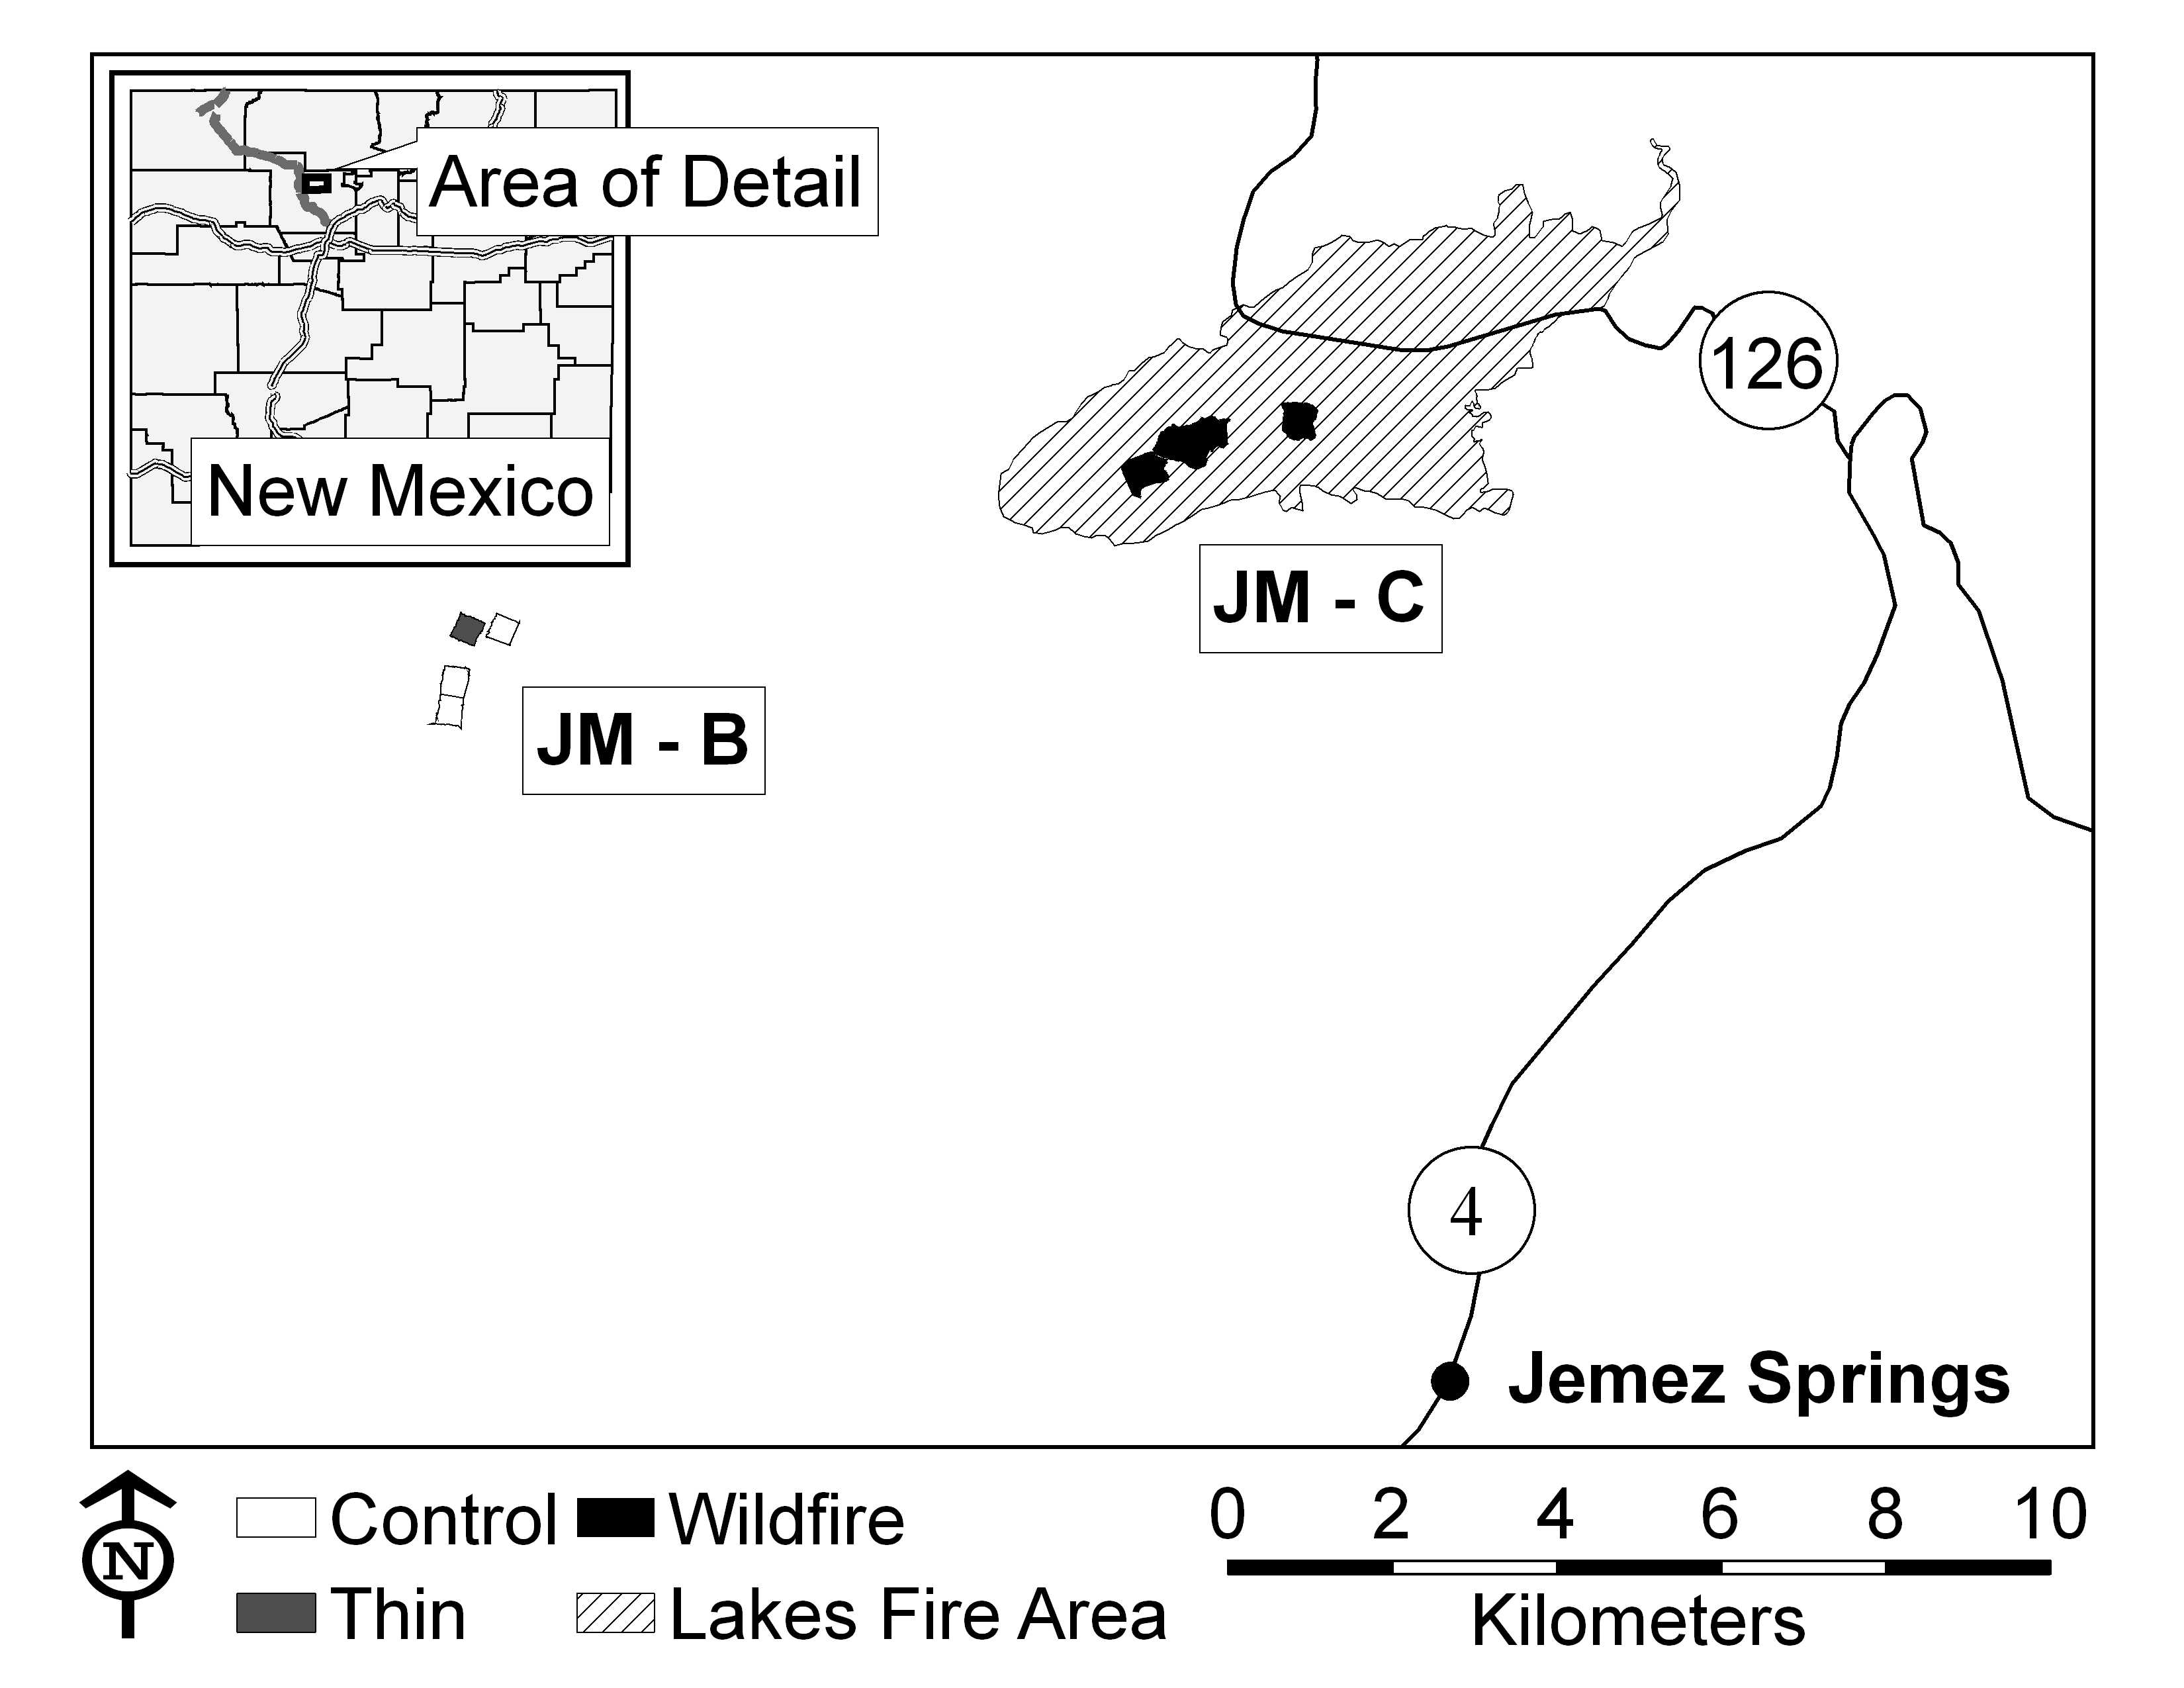
\includegraphics[height=4in,width=5.2in]{Ch14-Multisession/figs/converse_NM_Overview_4.jpg}
\end{center}
\caption{
Central New Mexico Study Area from \citet{converse_etal:2006jwm}.
}
\label{fig.studyarea}
\end{figure}



\begin{figure}[ht]
\begin{center}
\includegraphics[height=4.8in,width=6.5in]{Ch14-Multisession/figs/figure_V2.pdf}
\end{center}
\caption{
Abundance estimates for Peromyscus spp. per experimental unit
(with area = 5.0625 ha) for each of 24 groups composed of 8
experimental units in year 1 (groups 1:8), and the same 8
experimental units in year 2 (groups 9:16) and year 3 (groups 17:24)
(from \citet{royle_converse:2013}).
 Point estimates
(filled circles) are posterior modes, and error bars reflect 95\%
credible intervals. Also shown are the number of individuals
captured per group (open circles).  }
\label{fig.fig1}
\end{figure}

\end{comment}











\end{comment}

\chapter{Models for  Search-Encounter Data}
\markboth{Search-Encounter}{}
\label{chapt.search-encounter}

\vspace{0.3cm}


In this chapter we discuss models for search-encounter data. These
models are useful in situations where the locations of individuals are
observed directly by searching space in some fashion, rather than
biased by fixed trap locations. In most cases both detection
probability and parameters related to movement can be estimated using
such models. In the context of Bayesian analysis, we develop
search-encounter models conditional on movement outcomes, say
$u_{ik}$, the location of individual $i$ during sample occasion $k$.
The models we differentiate here depend on a number of things related
to data structure or survey protocol -- basically whether or not we
record the exact location and how we record it.

How exactly are search-encounter models different from models for data
from fixed arrays?  (1) sample units are either continuous space
polygons or lines, not points; (2) we have location information that
is not biased by trap locations (that is, restricted only to fixed
trap locations); (3) because we have direct observations of location
that exist independent of traps, we can often build an explicit model
of space usage or an explicit movement model.
% XXX RS: Couldn't you add your observation here, that with fixed arrays the movement model and the detection model are confounded? Actually, I think it might be necessary because we talk so much about movement models in the array models that without a little further info here it's not entirely clear why the movement models from search-encounter are different
Conversely, 
 when we have an array of fixed trap locations, the
movement process is completely confounded with the encounter process
because the list of potential observation locations is prescribed, a
priori, indendent of any underlying movement process.

A few distinct types of situations exist where these models come in
handy. The prototypical, maybe ideal, situation
\citet{royle_etal:2011mee} is where we have a single search path
through a region of space from which observations are made (just as in
the typical distance sampling situation, using a transect). As we walk
along the search path, we note the location of each individual that is
detected, {\it and their identity} (this is different from distance
sampling in that sense). 
Alternatively, we could delineate a search
area, and conduct a systematic search of that region. An example is
that of \citet{royle_young:2008}, which involved a plot search for
lizards. They assumed the plot was uniformly searched which justified
an assumption of constant encounter probability, $p$, for all individuals within the plot boundaries. 
The data set
was $\ge 1$ location observations for each of a sample of $n$
individuals.  The recent paper by \citet{efford:2011} discussed
likelihood analysis of similar models. In the terminology of \mbox{\tt
  secr} such models are referred to as models for {\it polygon
  detectors}.  The model described by \citep{royle_etal:2011mee} is a
generalization of the polygon search model, as we describe below.
% XX RS: You also gonna describe the transect model? Might be nice to add, if so. Something like in the other chapters, like, 'in this chapter... blabla'


\begin{comment}
%%## This argument here is basically true, but i'm not sure how to
%%package the idea yet.

Search-encounter models also provide something of a bridge between the
standard models for fixed trap arrays (e.g., Chapt. \ref{chapt.scr0}, etc.),
and the models described in Chapt. \ref{chapt.noID} in which individual
identity is not available. One one hand, in the standard fixed trap
array situation, we observe individual encounter data at each fixed
trap. In the ``no ID'' models, we observe trap-specific encounter
frequencies, but no individual identity. 
Search-encounter models are intermediate
in terms of the structure of the observable data.

\end{comment}


\section{Search-encounter sampling designs}

Before we discuss models for search-encounter data, we'll
introduce the types of sampling situations that
produce individual location data.  We imagine there are a lot more sampling protocols
than identified here, but these are some of the standard situations that we have
encountered over the last few years in developing applications of SCR
models.  For our purposes here we recognize 4 basic sampling designs,
each of which might have variations due to modification of the basic
sampling protocol. In later sections of this chapter we will explore some
examples involving of some of these situations. 

\subsection{Design 1: Fixed Search Path}
\label{searchencounter.sec.fixedpath}

The ideal situation is where we have a continuous search-path or
line, or multiple such lines, in some region
(Fig. \ref{searchencounter.fig.snakeline}). This is the type of
problem described by \citet{royle_etal:2011mee}. We assume the paths or
lines are laid out a priori in some manner that is done independent of
the activity centers of individuals and the collection of data does
not affect the lines.  That is, we assume the lines are established
{\it a priori} without consideration of factors that might affect
density. A situation in which this may be violated is when sampling is
based on sniffer dogs. A handler working a team of dogs is usually
letting the dogs ``follow their nose'', and the dogs are adapting to
their own senses as they work the landscape. 
In some cases the lines are within well-defined
polygons (shown in Fig. \ref{searchencounter.fig.snakeline}) but the
polygon boundaries may or may not be meaningful in terms of the
observation process. That is, if one is sampling along the path shown
in Fig. \ref{searchencounter.fig.snakeline} and recording locations of
individuals, then the boundary is not relevant if individual locations
may be recorded outside the polygon boundary. In this case, perhaps
the polygon boundary (quadrats in
Fig. \ref{searchencounter.fig.snakeline}) was used as a mechanism for
producing the transect, but does not affect the collection of data.  A
number of variations of this search encounter situation are possible,
and these produce slightly different data structures and corresponding
modifications to the model:
% XX RS: The list is not very intuitive. Why7when would we record the location on the transect where we first saw an individual? (1b) And in the CR-DS hybrid, don't wen use the distance to get at the location of the individual? I guess what's not quite clear here is: are these protocolls that lead to different data structures and thus, different models, or are these just different survey techniques to get at the same thing, namely individual locations
% Andy sez: Good point.  I added a phrase to above sentence but not
% sure what else to say. 
\begin{itemize}
 \item[] Protocol (1a). We know the search path and record the locations of individuals.
 \item[] Protocol (1b). We record the location of individuals and
   the location on the transect where we first observed the individual.
 \item[] Protocol (1c). We record
the closest perpendicular distance. This is a typical
   distance sampling situation, and this is a type of hybrid CR-DS model.
 \item[] Protocol (1d). In this case, observations are restricted to
   the line itself. We imagine that the line is evolving in response
   to search activity. 
 \end{itemize}


\begin{figure}
\centering
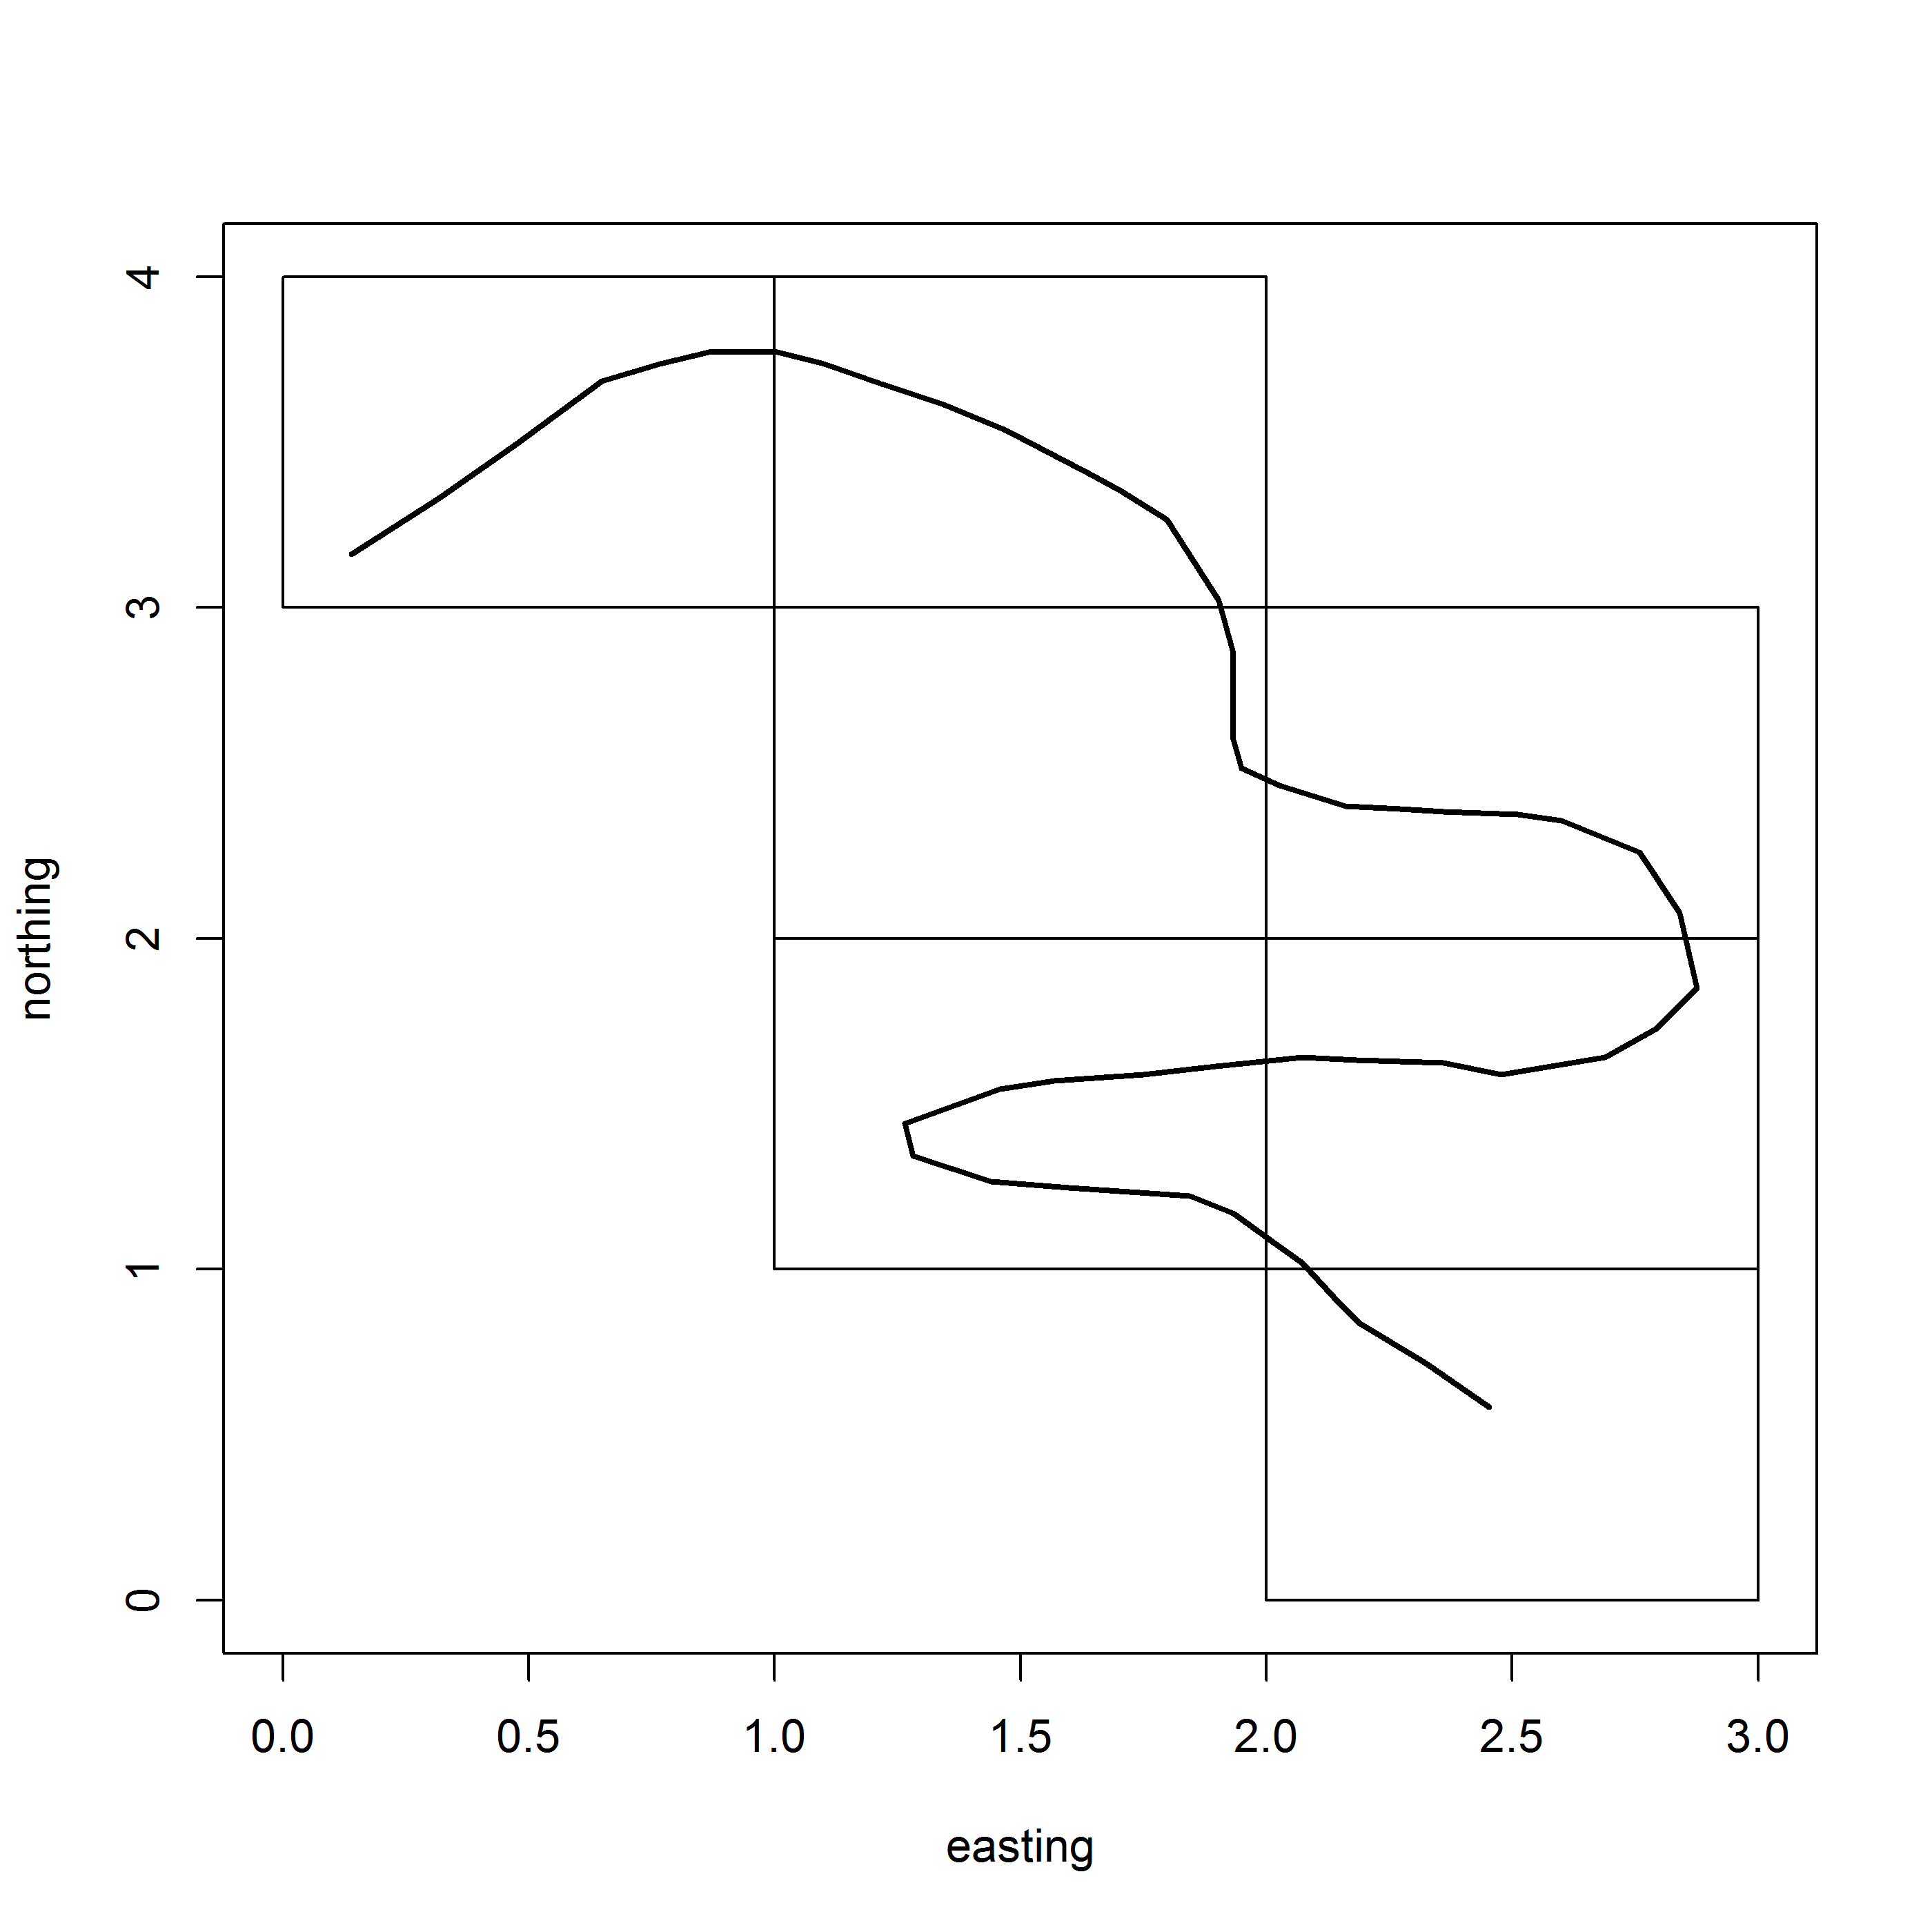
\includegraphics[width=4in,height=4in]{Ch15-searchencounter/figs/snakeline.png}
\caption{
A survey line through parts of 7 quadrats in a
  hypothetical landscape. An observer travels the transect and
  identifies individuals in the vicinity of the line, recording their
  identity and location.
}
\label{searchencounter.fig.snakeline}
\end{figure}


\subsection{Design 2: Uniform search intensity}

In this case we have one or more well-defined sample areas (polygons),
such as a quadrat or a transect, and we imagine that the area is
uniformly searched 
so that encounter probability is constant for all
individuals within the search area
(we'll abbreviate this as ``the USI model'').
 Sampling produces locations of
individuals within the well-defined boundaries of the sample area. The
polygon boundaries defining the sample unit are important because it
tells us that $p=0$ by design outside of the boundary.

Using the example from the Fig. \ref{searchencounter.fig.snakeline},
we imagine that each of the identified quadrats is uniformly searched,
which is to say, we assume that 
 each individual within the boundaries of the {\it quadrat}
has an equal probability of being detected.  In the context of
replicate sampling occasions (e.g., on consecutive days), individuals
may move on or off of the plot, and so individuals may have different
probabilities of being {\it available} to encounter, based on the
closeness of their activity center to the quadrat boundaries. However, given
that they're available, the USI model assumes they have constant
encounter probability. 
% XX RS: A couple of things here: I would point out that (if I
% understand that correctly) individuals don't have the same
% probability of being within the search path, though, because them
% being  there depends on how far away they live. Otherwise this
% statement is just a little confusing. 
% 
%% The other thing is: it is not really clear if you are referring to
%% the quadrats in the figure and are saying that these were searcher
%% uniformly (not along the line that snakes through the quadrats in
%% the figure, but actually uniformly), or that if you look at how
%% much of the line is in each quadrat, the amount of 'effort' is the
%% same - so search effort is distributed uniformly among the
%% quadrats. I think the confusion might come from talking about area
%% searches (so I am thinking about 2-d space) but then referencing
%% the search path (where I think 1-d). Maybe this section just needs
%% some definitions up front to make things clearer.
%
% Andy sez: I resolved these things I hope

In this USI situation, where we have contiguous quadrats,  the
individual quadrat boundaries are irrelevant as far as the model
specification goes,  and we
only need to be concerned about the ``total'' boundary of the
composite polygon (the intersection of all little ones). That said,
for analysis in {\bf BUGS}, it is easier to work with rectangular
polygons and so, from a practical standpoint, we might describe the
model in terms of each of the collection of smaller quadrats. It might also be advantageous
to ensure nice rectangular plot boundaries (or else write your own
MCMC algorithm, see Chapt. \ref{chapt.mcmc}).  We show a simulation
example for an area-search model below, and we analyze it both using a
bivariate normal model and a 2-d random walk type of model to describe
animal movement, i.e., the way individual locations ${\bf u}_{ik}$ are
generated. For further exampels and analyses, we refer you to
\citet{royle_dorazio:2008}, who reanalyzed the lizard data from
\citet{royle_young:2008}, and \citet{efford:2011ecol} and
\citet{marques_etal:2011}.

% XX RS: Would increase axis labels in the figure.
%% andy sez : needs done

\subsection{Partial Information Designs (3 and 4)}

In practice, we think many situations will arise in which partial
spatial information is available. The data structure and model are
slightly different in these cases.

{\bf Design 3}: We imagine that search polygons are defined
(e.g., the grid cells in Fig. \ref{searchencounter.fig.snakeline}) and
we record
locations of encountered individuals, but we do not perform a uniform search
of quadrats and we neglect to record the the search path. 
In this case, we don't have direct information on the observation
process -- we are not able to characterize the {\it probability of
  that specific observation} because, in general, it depends on the
precise configuration of the search path.  In this case, while it is
beneficial to have the location of the individual, we do lose some
information by not recording the points in space from which that
individual was detectable. This would be akin to neglecting to record
the trap locations in the standard situation of having a fixed array
of traps. 
% XX RS: It's not entirely clear to me: so we record individual locations, but we don't spread search effort uniformly and have no means of quantifying effort, is that it?I think it would help to be more explicit about why we need the search path, if we have the location of the individual, which is waht we're really interested in.
%% Andy sez: I embellished above. 

% XX RS - later: I understand now, but I think before or while you outline these protocols, it would be important to state what the different pieces are used for (without equations). So if we don't search an entire area, the path is essential because it tells us where we sampled and thus, where we were able to encounter individuals; also, the path locations are needed for the observation-by-distance model, if we want to specify one; and even if we assign detections to, e.g. grid cell centers, the path in each grid cell can tell us somethign about the search effort (analogous to how many days a camera trap was operational); and the locations of individuals are necessary to get at the movement model. Without these definitions it's hard to appreciate the differences in the data structure and they don't become fully clear until the end of section 2
What we have in these situations are
observations of individuals {\it and} the quadrat they were detected in,
but not the finer
scale ``movement'' outcomes.


{\bf Design 4}: In this we neglect to record a search line and also the locations of individuals
within the quadrats.  There are two variations of this:
\begin{itemize}
\item[] Protocol (4a) - You could have
counts by identified by individual within each quadrat. 
For example, if scats are collected and genetically assigned to individuals, and for each individual we get a count of scats in each quadrat.
\item[] Protocol (4b) - We don't have 
individual identities, but just total counts. This is the
\citet{chandler_royle:2013} model (Chapt. \ref{chapt.noID}).
\end{itemize}
It is possible also that we retain the survey line information, which
could possibly be used to identify a covariate of ``coverage'', in
order to account for different search effort in each quadrat.




\begin{comment}
\subsection{Examples}

The capricailie example: search of polygons -- could be search
encounter with uniform search intensity but we ignored the polygon
boundaries and just mapped each observation to the center point.  The
fisher data: we had a GPS line but it was not really fixed , it
evolved as dogs searched around. Therefore as a practical matter the
locations of samples were all {\it on} the line. We therefore mapped
to a center point of a grid. We make a grid of the sampled area and we
assume within each grid if a species is present then it is independent
.... actually if the grid is placed INDEPENDENT of the lines then its
probably safe to make some kind of independence assumption.  Russell
et al. -- similar situation, they have a search parth but not really
independent.

For the rest of this chapter, we will provide some model
formulations for some cases, provide code for simulating and analyzing
the data, and some real examples but not for every situation.
A number of published examples have been given. The Royle et al. 2011
paper on the MHB. The Royle and Young 2008 (see also Marques et
al. and Efford 2011). We also have the Thompson et al. XXX and Russell
et al. XXXX and Capricaillie paper XXXXX.

Possible examples to provide:

Example 1:  Analysis of the Swiss MHB survey using Design 1

Example 1b: Lizard data. No need to analyze this as it was done in RD book. Mention polygon detectors in secr.

Example 2: Fisher data possibly - lion data or -- or  Capricaillie data?
\end{comment}




\section{A Model for Search-Encounter Data}

We focus here on developing a model for Designs 1 and 2, as these
represent ideal sampling situations.  In contrast to most of the models
described in this book (but see Sec. \ref{poisson-mn.sec.acoustic}), we
develop models for encounter probability that depend explicitly on the
instantaneous location ${\bf u}_{ik}$, for individual $i$ at sample
occasion $k$: $p_{ik} \equiv p({\bf u}_{ik}) = \Pr(y_{ik}=1|{\bf
  u}_{ik})$.  Note that ${\bf u}$ is unobserved for the $y=0$
observations and thus we cannot analyze the conditional-on-${\bf u}$
likelihood directly. Instead, we regard ${\bf u}$ as random effects
and assume a model for them, which allows us to handle the
problem of missing ${\bf u}_{ik}$ values (described subsequently).
% XX RS: Maybe refer forward to the movement model that achieves this. 

To develop encounter probability models for this problem we cannot
just use the previous models because the ``trap'' is actaully a line
or collection of line segments (e.g.,
Fig. \ref{searchencounter.fig.snakeline}).  Intuitively,
$\Pr(y_{ik}=1|{\bf u}_{ik})$ should increase as ${\bf u}_{ik}$ comes
``close'' to the line segments ${\bf X}$. It seems reasonable to
express closeness by some distance metric $||{\bf u}_{ik} - {\bf X}
|| = dist( {\bf u}_{ik}, {\bf X})$ and then assume
\[
\mbox{logit}(p_{ik}) = \alpha_{0} + \alpha_{1} ||{\bf u}_{ik} - {\bf X}||.
\]
For the case where ${\bf X}$ describes a wandering line, some
kind of average distance from ${\bf u}$ to the line
might be reasonable; possible alternatives include the absolute
minimum distance or the mean over specific segments
of the line (within some distance), etc.  We could also have a model
without an explicit distance component, by assuming that individuals
within a certain distance from the search path are encountered with
equal probability. In this case, we have only a single parameter
$\alpha_{0}$ but must also specify the distance limit. 
% XX RS: technically, we could also assume that all individuals within a certain distance from the search path are encountered with equal prob., right?
% This more out of curiosity...
%% Andy sez: I added a thing above to suggest that. This is a good idea!

\subsection{Modeling total hazard to encounter}

Because the line {\bf X} is not a single point (like a camera trap) we
have to somehow describe the total encounter probability induced by
the line. A natural approach is to model the total hazard to capture
\citep{borchers_efford:2008}, which is standard in survival analysis,
and also distance sampling \citep{hayes_buckland:1983,
  skaug_schweder:1999}.  The individual is detected 
if encountered at any point along ${\bf X}$. Naturally,
covariates are modeled as affecting the hazard rate and we think of
distance to the line as a covariate acting on the hazard. Let $h({\bf
  u}_{ik},{\bf x})$ be the hazard of individual $i$ being encountered
by sampling at a point ${\bf x}$ on occasion $t$.  For example, one
possible model assumes, for all points ${\bf x} \in {\bf X}$,
\begin{equation}
\log(h({\bf u}_{ik},{\bf x})) = \alpha_{0} + \alpha_{1}*dist({\bf u}_{ik},{\bf x}).
\label{eq.hazard}
\end{equation}
Additional covariates could be included in the hazard function in the
same way as for any model of encounter probability that we've
discussed previously.  The total hazard to encounter anywhere along
the survey path, for an individual located at ${\bf u}_{ik}$, say
$H({\bf u}_{ik})$, is obtained by integrating over the surveyed line,
which we will evaluate numerically by a discrete sum where the hazard
is evaluated at the set of points ${\bf x}_{j}$ along the surveyed
path:
\begin{equation}
H({\bf u}_{ik}) =  \exp(\alpha_{0}) \left\{ \sum_{x_{j}}  \exp(\alpha_{1}*dist({\bf
    u}_{ik},{\bf x}_{j})) \right\}
\label{eq.totalhazard}
\end{equation}
where ${\bf x}_{j}$ is the $j^{th}$ row of ${\bf X}$ defining the
survey path as a collection of line segments which can be arbitrarily
dense, but should be regularly spaced.  Then the probability of
encounter on a given sampling occasion  
% XX RS: .. on a given occasion? That just made me think... would an
% occasion here be a repeated survey of the same search path? Might be
% good to define or discuss what occasions can mean in this context
% briefly. I geuss it could be a repeat visit, or a visit later in
% time to a different quadrat?
is
\begin{equation}
p_{ik} \equiv p({\bf u}_{ik}) = 1- \exp(-H({\bf u}_{ik})).
\label{search-encounter.eq.encounterprob}
\end{equation}
Its possible that the search path could vary by sampling occasion, say
${\bf X}_{k}$, which can easily be accommodate in the model simply by
calculating the total hazard to encounter for each distinct search
path.

This is a reasonably intuitive type of encounter probability model in
that the probability of encounter is large when an individual's
location ${\bf u}_{it}$ is close to the line in the average sense
defined by Eq. \ref{eq.totalhazard}, and vice versa.
Further, consider the case of a single survey point, i.e., ${\bf X} \equiv {\bf
  x}$, which we might think of as a camera trap location.  In this
case note that Eq. (\ref{search-encounter.eq.encounterprob}) is equivalent to
\[
\log(-\log(1-p_{ik})) = \alpha_{0} + \alpha_{1}*dist( {\bf u}_{ik},{\bf x})
\]
which is to say that distance is a covariate on detection that is
linear on the complementary log-log scale, which is similar to the
``trap-specific'' encounter probability of our Bernoulli encounter
probability model (see Chapt. \ref{chapt.scr0}).
The difference is that, here, the relevant distance
is between the ``trap'' (i.e. the survey lines) and the individual's
present location, ${\bf u}_{ik}$, which is observable. On the other
hand, in the context of camera traps, the distance is that between the
trap and a latent variable, ${\bf s}_{i}$, representing an
individual's home range or activity center which is not observed.


A key assumption of this formulation of the model is that 
encounters at each point along the line, ${\bf x}_{j}$, are
independent of each other point. Then, the event that an individual is
encountered {\it at all} is the complement of the event that it is not
encountered {\it anywhere} along the line \citep{hayes_buckland:1983}.
In this case, the probability of not being encountered at trap $j$ is:
 $1-p({\bf u}_{ik},{\bf x}_{j}) = exp(-h({\bf u}_{ik},{\bf x}_{j}))$
and so the probability that an individual is not encountered at all is
 $\prod_{j} exp(-h({\bf u}_{ik},{\bf x}_{j}))$. The encounter
probability is therefore the complement of this, which is precisely
the expression given by Eq. \ref{search-encounter.eq.encounterprob}.


Any model for encounter probability can be converted to a hazard model
so that encounter probability based on total hazard can be derived.
We introduced this model above:
\[
\log(h({\bf u}_{ik},{\bf x})) = \alpha_{0} + \alpha_{1}*\mbox{dist}({\bf u}_{ik},{\bf x}).
\]
which is usually called the Gompertz hazard function in survival
analysis, and it is most often written as $h(t) = a \exp( b*t)$ in which
case $log(h(t)) = log(a) + b*t$.  
% XX RS: I really don't know anything about these models, so excuse my ignorance... but do these survival models use any kind of covariate (where we use distance)? Here it sounds like they use distance as a covariate, which is not very intuitive...
Model 2 (squared-distance) is a
quadratic function of distance
\[
\log(h({\bf u}_{ik},{\bf x})) = \alpha_{0} + \alpha_{1}*\mbox{dist}({\bf u}_{ik},{\bf x})^2.
\]
We've used this type of Gaussian kernel model 
quite a bit in the book, and it implies a
bivariate normal hazard rate. \citet{borchers_efford:2008} use this model:
\[
h({\bf u}_{ik},{\bf x} ) = -\log(1 - \mbox{expit}(\alpha_{0})
\exp( \alpha_{1}*\mbox{dist}({\bf u}_{ik},{\bf x})^2 ) )
\]
which produces a normal kernel model for {\it probability of
  detection} at the point level. i.e., $\Pr(y=1) = 1-\exp(-h) = h_{0}
\exp( \alpha_{1}*\mbox{dist}({\bf u}_{ik},{\bf x})^2 )$ where $h_{0} =
\mbox{logit}^{-1}(\alpha_{0})$.  
Another model is:
\[
\log(h({\bf u}_{ik},{\bf x})) = \alpha_{0} + \alpha_{1}*\log(\mbox{dist}({\bf u}_{ik},{\bf x}))
\]
which is a Weibull hazard function.



\subsection{Modeling movement outcomes}

We have so far described the model for the encounter data in a manner
that is conditional on the locations ${\bf u}_{ik}$, some of which are
unobserved. Naturally, we should specify a model for these latent
variables -- i.e., a movement model -- so that we could either do a
Bayesian analysis by MCMC \citep{royle_young:2008, royle_etal:2011} or
compute the marginal likelihood \citep{efford:2011}.  To develop such
a model, we adopt what is now customary in SCR models -- we assume
that individuals are characterized by a latent variable, ${\bf
  s}_{i}$, which represents the activity center.  This leads to some
natural models for the movement outcomes ${\bf u}_{ik}$ conditional on
the activity center ${\bf s}_{i}$. Here we make use of the bivariate
normal model (but see below for alternatives):
\[
 {\bf u}_{ik} | {\bf s}_{i} \sim \mbox{BVN}({\bf s}_{i}, \sigma^{2}{\bf I}),
\]
where ${\bf I}$ is the $2\times 2$ identity matrix.  
% XX RS: In the partial ID chapter we use a different notation for the
% BVN model; we use \Sigma, and then define that as a 2x2 matrix with
% 0 and sigma^2.... thinking about it, these two notations are pretty
% similar... do you think we should point out that they're the same? 
%%% Andy sez: I will start using BVN( )  
This is a primitive model of individual movements about their home
range but we believe it will be adequate in many capture-recapture
studies which are often limited by sparse data.

We adopt our default assumption for the activity centers ${\bf s}$:
\[
 {\bf s}_{i} \sim \mbox{Uniform}({\cal S}); \; \; i=1,2,\ldots,N.
\]
The usual considerations apply in specifying the state-space ${\cal
  S}$ -- either choose a large rectangle, or prescribe a habitat mask
to restrict the potential locations of ${\bf s}$.



\subsection{Simulation and analysis in {\bf JAGS}}

Here we will simulate a sample data set that goes with the situation
desccribed in Fig. \ref{searchencounter.fig.snakeline} and then
analyze the data in {\bf JAGS}.  We begin by defining the state-space
containing all of the sample boxes in
Fig. \ref{searchencounter.fig.snakeline} and a total population which
is going to be 4 individuals per unit quadrat ($1 \times 1$). We use a
rectangular state-space here for convenience:
% XX RS: Either the numbers below are off or you mean a rectangular S
% Andy sez:  yea I think so 
\begin{verbatim}
> xlim <- c(-1, 4)
> ylim <- c(-1, 5)
> perbox <- 4
> N <- 30*perbox   # Total of 30 1x1 quadrats
\end{verbatim}
The line in Fig. \ref{searchencounter.fig.snakeline} is an irregular
mesh of points obtained by an imperfect manual point-and-clicking
operation, which probably mimics many actual situations including the
way in which GPS points come to us. In order to apply our model we
need a regular mesh of points. We can obtain a regular mesh of points
from the irregular mesh by using some functions in the packages
\mbox{\tt rgeos} and \mbox{\tt sp}, especially the function \mbox{\tt
  sample.Line}, as follows:
\begin{verbatim}
> library(rgeos)
> library(sp)
> line1 <- source("line1.R")

> line1 <- as.matrix(cbind(line1$value$x,line1$value$y))
> points <- SpatialPoints(line1)

> sLine <- Line(points)
> regpoints <- sample.Line(sLine,250,type="regular")  # Key step!
\end{verbatim}
Next, we set a random number seed, simulate activity centers and set
some model parameters required to simulate encounter history data.
Note, the commands for doing all of this and plotting the results are given
in the function \mbox{\tt snakeline} in the {\bf R} package
\mbox{\tt scrbook}. 
In the following commands you can see where the
regular mesh representation of the sample line is extracted from the
\mbox{\tt regpoints} object which we just created:
{\small
\begin{verbatim}
> set.seed(2014)
> sx <- runif(N,xlim[1],xlim[2])
> sy <- runif(N,ylim[1],ylim[2])

> sigma.move <- .35
> sigma <-.4
> alpha0 <- .8
> alpha1 <- 1/(2*(sigma^2))
> X <- regpoints@coords
> J <- nrow(X)
\end{verbatim}
}

Next we're going to simulate data. We do this basically in 2 steps:
For each individual in the population and for each of $K$ sample
occasions, we simulate the location of the individual as a bivariate
normal random variable with mean ${\bf s}_i$ and $\sigma = 0.25$ ({\tt
  sigma.move} in the code above). Next, we compute the encounter
probability model using Eq. \ref{search-encounter.eq.encounterprob},
with the bivariate normal hazard model, 
and then retain the data objects corresponding to individuals that get
captured at least once. All of this goes according to the following
commands: 
{\small
\begin{verbatim}
> K <- 10   ##  Sample occasions = 10
> U <- array(NA,dim=c(N,K,2))  ## Array to hold locations
> y <- pmat <- matrix(NA,nrow=N,ncol=K)  ## Initialize
> for(i in 1:N){
+ for(k in 1:K){
+   U[i,k,] <- c(rnorm(1,sx[i],sigma.move),rnorm(1,sy[i],sigma.move))
+   dvec <- sqrt( ( U[i,k,1] - X[,1])^2 + (U[i,k,2] - X[,2])^2  )
+   loghaz<- alpha0 - alpha1*dvec*dvec   
+   H <- sum(exp(loghaz))
+   pmat[i,k] <- 1-exp(-H)
+   y[i,k] <- rbinom(1,1,pmat[i,k])
>   }
> }
> Ux <- U[,,1]
> Uy <- U[,,2]
> Ux[y==0] <- NA
> Uy[y==0] <- NA
\end{verbatim}
}

In this code above, we define matrices, \mbox{\tt Ux} and
\mbox{\tt Uy}, that hold the 
observed locations of individuals during each occasion. Note that, if
an individual is {\it not} captured, we set the value to \mbox{\tt
  NA}. We pass these partially observed objects to {\bf JAGS} to fit
the model. 

Finally, we do the data augmentation and we make up some starting
values for the location coordinates that are missing. 
 For these, we
cheat a little bit (for convenience and hopefully to improve the
efficiency of the MCMC for the simulated data sets) and use the actual
activity center values. In practice, we might think about using the
average of the observed locations.
{\small
\begin{verbatim}
> ncap <- apply(y,1,sum)
> y <- y[ncap>0,]
> Ux <- Ux[ncap>0,]
> Uy <- Uy[ncap>0,]

> M <- 200
> nind <- nrow(y)
> y <- rbind(y,matrix(0,nrow=(M-nrow(y)),ncol=ncol(y)))
> Namat <- matrix(NA,nrow=(M-nind),ncol=ncol(y))
> Ux <- rbind(Ux,Namat)
> Uy <- rbind(Uy,Namat)
> S <- cbind(runif(M,xlim[1],xlim[2]),runif(M,ylim[1],ylim[2]))
> for(i in 1:nind){
+     S[i,] <- c( mean(Ux[i,],na.rm=TRUE),mean(Uy[i,],na.rm=TRUE))
> }
> Ux.st <- Ux
> Uy.st <- Uy
> for(i in 1:M){
+     Ux.st[i,!is.na(Ux[i,])]<-NA
+     Uy.st[i,!is.na(Uy[i,])]<-NA
+     Ux.st[i,is.na(Ux[i,])]<-S[i,1]
+     Uy.st[i,is.na(Uy[i,])]<-S[i,2]
> }
\end{verbatim}
}

The {\bf BUGS} model specification is shown in Panel 
\ref{search-encounter.panel.design1}, although we neglect the standard
steps showing how to 
bundle the data, inits, and farm
all of this stuff out to {\bf JAGS} (see the help file for \mbox{\tt
  snakeline})for the whole script.

\begin{panel}[htp]
\centering
\rule[0.15in]{\textwidth}{.03in}
{\small
\begin{verbatim}
model {

# Priors
alpha0~dunif(-25,25)
alpha1~dunif(0,25)

lsigma~dunif(-5,5)
sigma.move<-exp(lsigma)
tau<-1/(sigma.move*sigma.move)
psi~dunif(0,1)

# Likelihood
for(i in 1:M){ # Loop over individuals
 z[i]~dbern(psi)
 s[i,1]~dunif(xlim[1],xlim[2])
 s[i,2]~dunif(ylim[1],ylim[2])
 for(k in 1:K){ # Loop over temporal replicates
    u[i,k] ~ dnorm(s[i,1],tau)
    v[i,k] ~ dnorm(s[i,2],tau)
    for(j in 1:J){ # Loop over each point defining line segments
      d[i,k,j]<-  pow(pow(u[i,k]-X[j,1],2) + pow(v[i,k]-X[j,2],2),0.5)
      h[i,k,j]<-exp(alpha0-alpha1*d[i,k,j]*d[i,k,j])
   }
   H[i,k]<-sum(h[i,k,1:J])
   p[i,k]<- z[i]*(1-exp(-H[i,k]))
   y[i,k] ~ dbern(p[i,k])
 }
}

# Derived quantity
N<-sum(z[])
}
\end{verbatim}
}
\rule[-0.15in]{\textwidth}{.03in}
\caption{
{\bf BUGS} model specification for the search-encounter model, based
on that from \citet{royle_etal:2011mee}. 
See the 
help file \mbox{\tt ?snakeline} for the {\bf R} code to simulate data
and fit this model. 
}
\label{search-encounter.panel.design1}
\end{panel}


Simulating the data as described above, and fitting the model in Panel
\ref{search-encounter.panel.design1} produces the results in Table
XXXXXXXXXXXXX: (soon to table-ize)

{\small
\begin{verbatim}
> wbout2
Inference for Bugs model at "model0.txt", fit using jags,
 3 chains, each with 3500 iterations (first 500 discarded)
 n.sims = 9000 iterations saved
            mu.vect sd.vect     2.5%      25%      50%      75%    97.5%  Rhat n.eff
N           117.626   5.675  107.000  114.000  117.000  121.000  129.000 1.015   160
alpha0        1.305   0.494    0.425    0.966    1.280    1.609    2.387 1.009   330
alpha1        3.806   0.423    3.050    3.519    3.777    4.073    4.733 1.008   310
psi           0.587   0.044    0.501    0.558    0.588    0.618    0.673 1.006   400
sigma.move    0.347   0.008    0.332    0.342    0.347    0.352    0.364 1.023    97
deviance   1146.513  32.059 1085.023 1124.098 1146.470 1167.643 1211.077 1.014   160

For each parameter, n.eff is a crude measure of effective sample size,
and Rhat is the potential scale reduction factor (at convergence, Rhat=1).

DIC info (using the rule, pD = var(deviance)/2)
pD = 507.5 and DIC = 1654.0
DIC is an estimate of expected predictive error (lower deviance is better).
\end{verbatim}
}


\subsection{Hard plot boundaries}

The previous development assumed that locations of individuals can be
observed anywhere in the state-space, determined only by the encounter
probability model as a function of distance from the search path.
However, in many situations, we might delineate a plot which restricts
where individuals might be observed (as in the situation considered by
\citet{royle_young:2008}).  For such cases we truncate the encounter
probability function at the plot boundary, according to:
\begin{equation}
p({\bf u}_{ik}) = (1- \exp(-H({\bf u}_{ik}))) \mbox{I}({\bf u}_{ik} \in {\cal X})
\label{search-encounter.eq.hardplot}
\end{equation}
where ${\cal X}$ is the surveyed polygon and the indicator function
$\mbox{I}({\bf u}_{ik} \in {\cal X}) = 1$ if ${\bf u}_{ik} \in {\cal
  X}$ and 0 otherwise.  That is, the probability of encounter is
identically 0 if an individual is located {\it outside} the plot at
sample period $t$.  We demonstrated how to do this in the {\bf BUGS}
language below for a model of uniform search intensity (area-search
model).



\section{Unstructured spatial surveys}

We identified a number of variations (``Protocols'') of the basic search-encounter
situation based on a survey line
(see Sec. \ref{searchencounter.sec.fixedpath}). 
Protocol 1d is what we'll refer to as 
 ``unstructured survey data'' and this seems to be fairly common in practice
\citep{thompson_etal:2012, russell_etal:2012}. 
In this protocol, the survey line evolves in response to information
about animal presence, which could be both the number of unique
individuals or the amount of sign in the local search area. The
motivating problem has to do with dog-team searches in which the dogs
usually wander around hunting scat, and their search path is based on
how they perceive the environment and what they're smelling. 
This violates the main assumptions that the line is placed a priori,
independent of density and unrelated to detectability.
The analysis framework implemented by
\citet{thompson_etal:2012} and \citet{russell_etal:2012} is based on
chopping the survey region into grid cells and using the center point
of the grid cell as an effective trap.  The heuristic argument to
support doing this is that if you pick the grid cells 
 larger than you think the dog team might be
responding to, and then treat the center point as a trap.  
The deficiency with this approach is that some of the ``sub-grid''
resolution information about movement is lost, so we probably lose
precision about any parameters of the movement model. 

\subsection{Mountain lions in Montana}

\citet{russell_etal:2012} analyzed mountain lion ({\it Puma concolor})
encounter history data to assess the status of mountain lions in the
Blackfoot Mountains of Montana.  The data collection was based on
opportunistic searching by hunters who shoot them with a
biopsy dart, and extract the DNA from the tissue sample. 
 They used 5 km $\times$ 5 km grid cells for
binning the encounters, and the length of the search path in each grid
cell as a covariate of effort that each grid cell was searched.  The
model is the Gaussian hazard model with baseline encounter probability
that depended on sex and effort in each grid cell, on the log scale:
\[
 \log(\lambda_{0,ij}) = \alpha_{0} + \alpha_{2} \log(C_{j}) + \alpha_{3} \mbox{Sex}_{i}
\]
Note for grid cells that were not searched, $C_{j} =0$, and those
probabilities were set to 0 in evaluation of the probability of
encounter.

\subsection{Tiger density in the Bandipur tiger reserve}

\citet{gopalaswamy_etal:2012ecol} reported on a study in the Bandipur
tiger reserve in India, where the objective was to obtain a population
size estimate for the reserve based on camera trapping and DNA
sampling of scats.  They had a camera trapping network, a standard
type of passive detector array, and they also had scat searches along
18 scat routes of a total length of 233.2 km. They created 237
segments of approximately 1 km each and used the center points of
these segments as traps. Effectively they mimic the search encounter
design 1 but, here, scats are only obtained on survey routes.
There is an issue of whether sampling along routes produces some kind
of a bias but, generally speaking, tigers aren't producing scats
randomly on the landscape according to the model either.

\subsection{Sierra National Forest Fisher Study}

Here we consider a more detailed example and provide the data and R
script for this analysis. 
The data come from an analysis of individual encounter histories of
the fisher ({\it Martes pennanti} by \citet{thompson_etal:2012}. Data
were collected by sniffer dogs searching space. The dogs were given
considerably latitude to determine their route.
Thus, the seearch path is not laid out a
priori but rather evolves haphazardly.  Strictly speaking it is
somewhat informed by what the dog senses at a very local scale. Maybe
(hypothetically, lets say) 
50 m or maybe 100 m.
So the idea here is to ingore the actual search path information
intentionally and do some spatial aggregation at a scale which we
think is larger than what the dogs are queuing into.......

Thompson et al. divided the region into 1 km polygons,

R function: \mbox{\tt SCRfisher  } produces the following results:

%% KIMMY put this in a table
{\small
\begin{verbatim}
Inference for Bugs model at "modelfile.txt", fit using WinBUGS,
 3 chains, each with 6000 iterations (first 1000 discarded)
 n.sims = 15000 iterations saved
          mean    sd 2.5%   25%   50%   75% 97.5% Rhat n.eff
psi        0.5   0.3  0.1   0.3   0.5   0.8   1.0    1   110
sigma      4.8   2.9  0.2   2.3   4.8   7.3   9.7    1   820
N        269.7 140.0 26.0 153.0 265.0 394.0 497.0    1   110
lam0       0.0   0.0  0.0   0.0   0.0   0.0   0.0    1   200
alpha      0.2   0.2  0.0   0.1   0.1   0.3   0.6    1  3500
deviance  72.6   7.6 54.2  68.8  73.9  77.9  84.0    1   210

For each parameter, n.eff is a crude measure of effective sample size,
and Rhat is the potential scale reduction factor (at convergence, Rhat=1).

DIC info (using the rule, pD = var(deviance)/2)
pD = 28.8 and DIC = 101.4
DIC is an estimate of expected predictive error (lower deviance is better).
\end{verbatim}
}


\section{Analysis of other protocols}

We previousl identified 4 distinct protocols of the Design 1
search-encounter model.
In the situation elaborated on above (what we called ``Protocol 1a''), the sample path is used to
locate individuals and, whether or not an individual is encountered,
is a function of the total hazard to encounter along the whole line.
We think there are a number of variations of this basic design that
might arise in practice.
A slight variation (what we called Protocol 1b) is based on 
recording location of individuals and also the location on the transect
where we observed the individual.  The probability of encounter is the
probability of encounter prior to point $x_{0}$ on the line
\citep{skaug_schweder:1999} and there is a slight modification to the
encounter probability model to account for that. This is exactly a
distance-sampling observation model, but with an additional
hierarchical structure the describes the individual locations about
their activity centers.  Protocol 1c is a slight variation of this --
instead of recording the point on the line where the individual was
first detected, we use, instead, the point on the line that has the
shortest perpendicular distance. This is a classical distance sampling
observation model, and it represents an intentional misspecification
of the model but it seems that the effect of this is relatively minor,
or, otherwise, we imagine people wouldn't do it.

\section{Design 2: Uniform Search Intensity}

A special case of a search-encounter type of model arises when its
possible to subject a quadrat (or quadrats) to a uniform search
intensity. This could be interpreted as an exhaustive search, or
perhaps just a thorough systematic search of the avaialable habitat.
The example considered by \citet{royle_young:2008} involved searching
of a 9 ha plot for horned lizards Fig.
\ref{searchencounter.fig.hornylizard} by a crew of
several people. It was felt in that case that complete coverage of
the plot was achieved. In general, however, we think you could have
a random sample of the plot and approximate that as a uniform coverage
-- this is kind of a design-based argument justifying the uniform
search intensity model. (we haven't simulated this situation, but it
would be worth checkign that out).

\begin{figure}
\centering
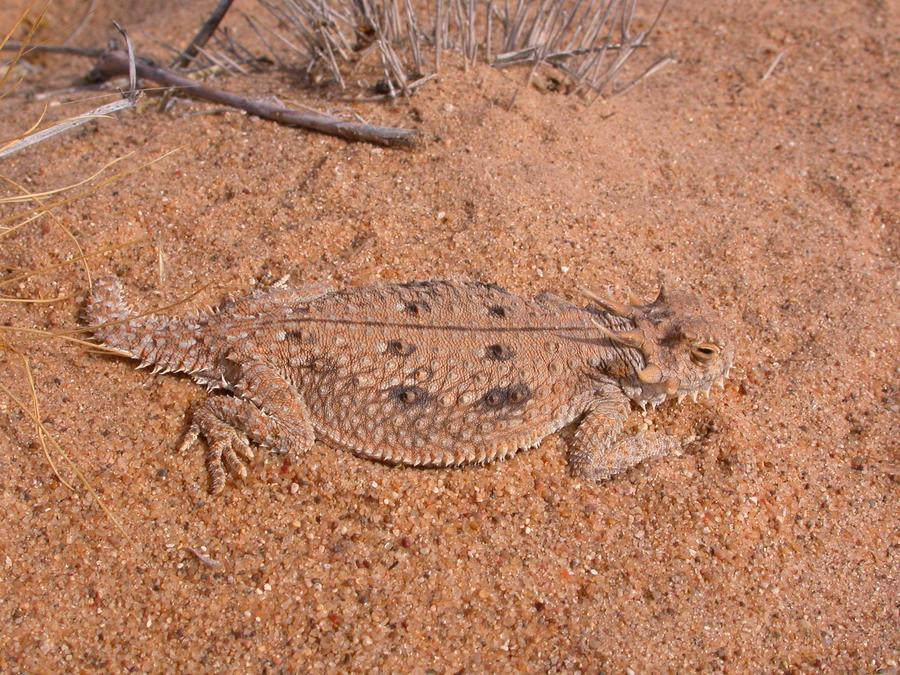
\includegraphics[width=3.6in,height=2.7in]{Ch15-searchencounter/figs/horny_lizard.jpg}
\caption{A flat-tailed horned lizard showing its typical cryptic
  appearance in its native environment.  Detection of flat-tailed
  horned lizards is difficult because they do not run when
  approached. Instead they shuffle under the sand or press down and
  remain motionless as shown in the picture.  The horns are employed
  only as a last resort if the camouflage fails.  {\it Photo credit:
    Kevin and April Young} }
\label{searchencounter.fig.hornylizard}
\end{figure}

It is clear that this uniform search intensity model is a special case
of the more general search encounter model in the sense that the
probability of encounter of an individual is a constant $p_{0}$ {\it
  if} the individual is located in the polygon ${\cal X}$ during
sample occasion $k$, i.e.,
\[
p({\bf u}_{ik}) = p_{0} \mbox{I}({\bf u}_{ik} \in {\cal X})
\]
which resembles Eq. \ref{search-encounter.eq.hardplot} except
replacing the encounter probability function with constant $p_{0}$.

In the analysis of \citet{royle_young:2008}, a simple bivariate
Gaussian movement model was used, in which
\[
 {\bf u}_{ik} | {\bf s}_{i} \sim \mbox{Normal}({\bf s}_{i}, \sigma^{2}{\bf I}),
\]
However, clearly more general versions of the model can be developed.
For example, imagine a situation where the successive samples of a
bounded sample polygont are relatively close together in time so that
successive locations of individuals are not well-approximated by the
independence model. Naturally we might consider using an
auto-regressive or random-walk type of model in which the successive
coordinate locations of individual $i$ behave as follows:
\begin{eqnarray*}
 u_{1}(i,k) | u_{1}(i,k-1) &\sim &  \mbox{Normal}( u_{1}(i,k-1),  \sigma^{2}) \\
 u_{2}(i,k) | u_{2}(i,k-1) &\sim &  \mbox{Normal}( u_{2}(i,k-1),  \sigma^{2}) \\
\end{eqnarray*}
here we use the notation $u_{1}$ and $u_{2}$ for the easting and
northing coordinates, respectively. (to keep from cluttering things up
with too many subscripts we have $i$ and $k$ as parenthetic arguments
here).   In addition, we require that the initial locations have a
distribution and, for that, we might being with a simple model such as
the uniformity model:
\[
 {\bf u}(i,1) \sim \mbox{Uniform}({\cal S})
\]
which effectively takes the place of the model for ${\bf s}_{i}$ that
we typically use. Under this model, individuals dont' have an activity
center but, rather, they drift through space more-or-less randomly
based just on their previous location. See \citet{ovaskainen:2004,
  ovaskainen:2008} see also our discussion of a similar model that
might arise in acoustic surveys (Sec. \ref{poisson-mn.sec.acoustic}).

We could allow for dependent movements about a central location ${\bf
  s}_{i}$ using an AR(1) or similar type of
model with parameter $\rho$, e.g.,
\[
 {\bf u}(i,k) | {\bf s}_{i} \sim   \mbox{BVN}( \rho*( {\bf u}(i,k-1) - {\bf s}_{i} ),  \sigma^{2} {\bf I}).
\]


In the \mbox{\tt scrbook} package, we provide a script for simulating
and fitting search-encounter data using the iid Gaussian model and
also the random walk model. We encourage you to adapt these to fit the
AR(1) movement model.  The {\bf BUGS} model specification is shown in
Panel \ref{search-encounter.panel.uniform} for the random walk
situation.  Of course we imagine that resouorce selection perhaps
using similar ideas to those dexcribed in Chapt. \ref{chapt.rsf} could
be parameterized in this movement model as well. In this case we set
up the run with JAGS using the standard commands. We did not specific
starting valules for the missing coordinate locations although we
imagine that JAGS should perform better if we provide decent starting
values. e.g., the last observed location or something.

\begin{verbatim}
R CODE FOR SIMULATING THIS SITUATION.....................?

To be inserted
\end{verbatim}


\begin{panel}[htp]
\centering
\rule[0.15in]{\textwidth}{.03in}
{\small
\begin{verbatim}
model{
psi ~ dunif(0,1)
tau ~ dgamma(.1,.1)
p0 ~ dunif(0,1)
sigma.move <- sqrt(1/tau)

# Likelihood
for (i in 1:M){
  z[i] ~ dbern(psi)
  G[i,1,1] ~ dunif(0,16)
  G[i,1,2] ~ dunif(0,16)

   for (t in 2:n.occasions){
## See here I can only make a model for LOCATION
      G[i,t,1] ~ dnorm(G[i,t-1,1], tau)
      G[i,t,2] ~ dnorm(G[i,t-1,2], tau)
# Test whether the actual location is in- or outside the study area. Needs to be done for each grid cell
    }
   for(t in 1:n.occasions){
      inside[i,t] <- step(G[i,t,1]-3) * step(13-G[i,t,1]) *step(G[i,t,2]-3) * step(13-G[i,t,2])
      Y[i,t] ~ dbern(mu2[i,t])
      mu2[i,t] <- p0 * inside[i,t] * z[i]
      } #t
   } #i
N <- sum(z[])
}
\end{verbatim}
}
\rule[-0.15in]{\textwidth}{.03in}
\caption{
{\bf BUGS} model specification for the search-encounter model similar
to Royle and Young 2008 but with a random walk movement model.
help file \mbox{\tt ?search$\_$encounter} in the {\bf R} package \mbox{\tt scrbook}.
}
\label{search-encounter.panel.uniform}
\end{panel}

\subsection{Movement and Dispersal in Open Populations}

In Chapt. \ref{chapt.open} we discuss many aspects of modeling open
populations, including some aspects of modeling movement and dispersal
and the relevance of SCR models to these problems. However, given the
introduction of the search-encounter model above, this is celarly
relevant to modeling movement and dispersal in open populations.  In
particular, the model described in Panel
\ref{search-encounter.panel.uniform} could easily be adapted to an
open population by conditioning on the first, and introducing a latent
``alive state'' with survival parameter $\phi_{t}$. This would be a
spatial version of the standard Cormack-Jolly-Seber model
(Chapt. \ref{open.sec.cjs})\footnote{Some work related to this is
  currently being carried out by our colleagues Torbjorn Ergon and
  Michael Schaub.}.

\section{Designs 3 and 4: Partial Information}


Design 1 and Design 2 (USI) are ideal in the sense that they product
both precise locations of individuals and also a precise
charachterization of the manner in which individuals are encountered
by sampling space. 

We have seen a number of studies that, in an ideal world, would have
generated data of a ``Design
1'' type but, for some practical reason or other reason, the model described
above cannot be used.
 We discuss some of these problems here, which all seem to involve a
 design type 1 but with partial information. We imagine there could be
 3 distinct situations
\begin{itemize}
\item[(a)] search path not recorded, locations recorded
\item[(b)] search path recorded, locations not recorded
\item[(c)] search path not recorded, locations not recorded [but plot of
detection is known]  {\bf Capercaillie}
\end{itemize}

For analysis of these search-encounter designs with partial information,
we think there are a number of options depending on the situation:
For (a) you could always assume uniform search intensity ,
which is probably ok if plots were randomly searched.
It would be useful to do a simulation study to look at how bad that
model is if plots were systematically or randomly searched, and with
heterogeneity in search intensity.
For (b), maybe you could map the locations to the center of each plot,
think of the plot as effective traps, and maybe use the search path
length as a covariate, or some measure of coverage of the
plot. Intuitively, this would be a decent solution of the plots are
small relative to typical home range sizes.
For (c) , same thing -- map the locations to the center of the plot,
but now you don't have a covariate of how much effort when into each
plot.


\subsection{Capricaillie status in Switzerland}

Variations on this theme have appeared in a number of papers.  (1)
\citet{mollet_etal:2012}, who obtained a population size estimate of a
large forest grouse species known as the capracaillie ({\it Tetrao
  urogallus}) in Switzerland.  The base SCR model is the Poisson model
(Chapt. \ref{chapt.poisson-mn}). Forest stands were searched by
observers for scat, which was analyzed for DNA identification of
individuals.  A total of 78 spatial units of a few ha each were
searched.  In this example, forest stands were searched but the search
path data was not available, only the unit in which each scat was
found.  It was searched in an expert manner, and it was believed that
a uniform search intensity model could be reasonable.  Importantly,
the sample units are actually large forest patches on the order of
tens of ha each, but variable in size. Data were {\it not} collected
by coordinates of observations but rather just recorded to the
specific patch in which the observation was encountered. To accomodate
this we defined ${\bf s}_{i}$ to be a discrete random variable taking
on values.  Forest patches were searched for scat which was situation
in which discrete patches of habitat are searched using some method
and it might be convenient (or occur inadvertently) to associate
samples to the patch level instead of recording observation
locations. In this case we might use a model $s[i] \sim dcat(probs[])$
where $probs[]$ are the probabilities that an individual inhabits a
particular patch.

\begin{comment}
\begin{figure}
\centering
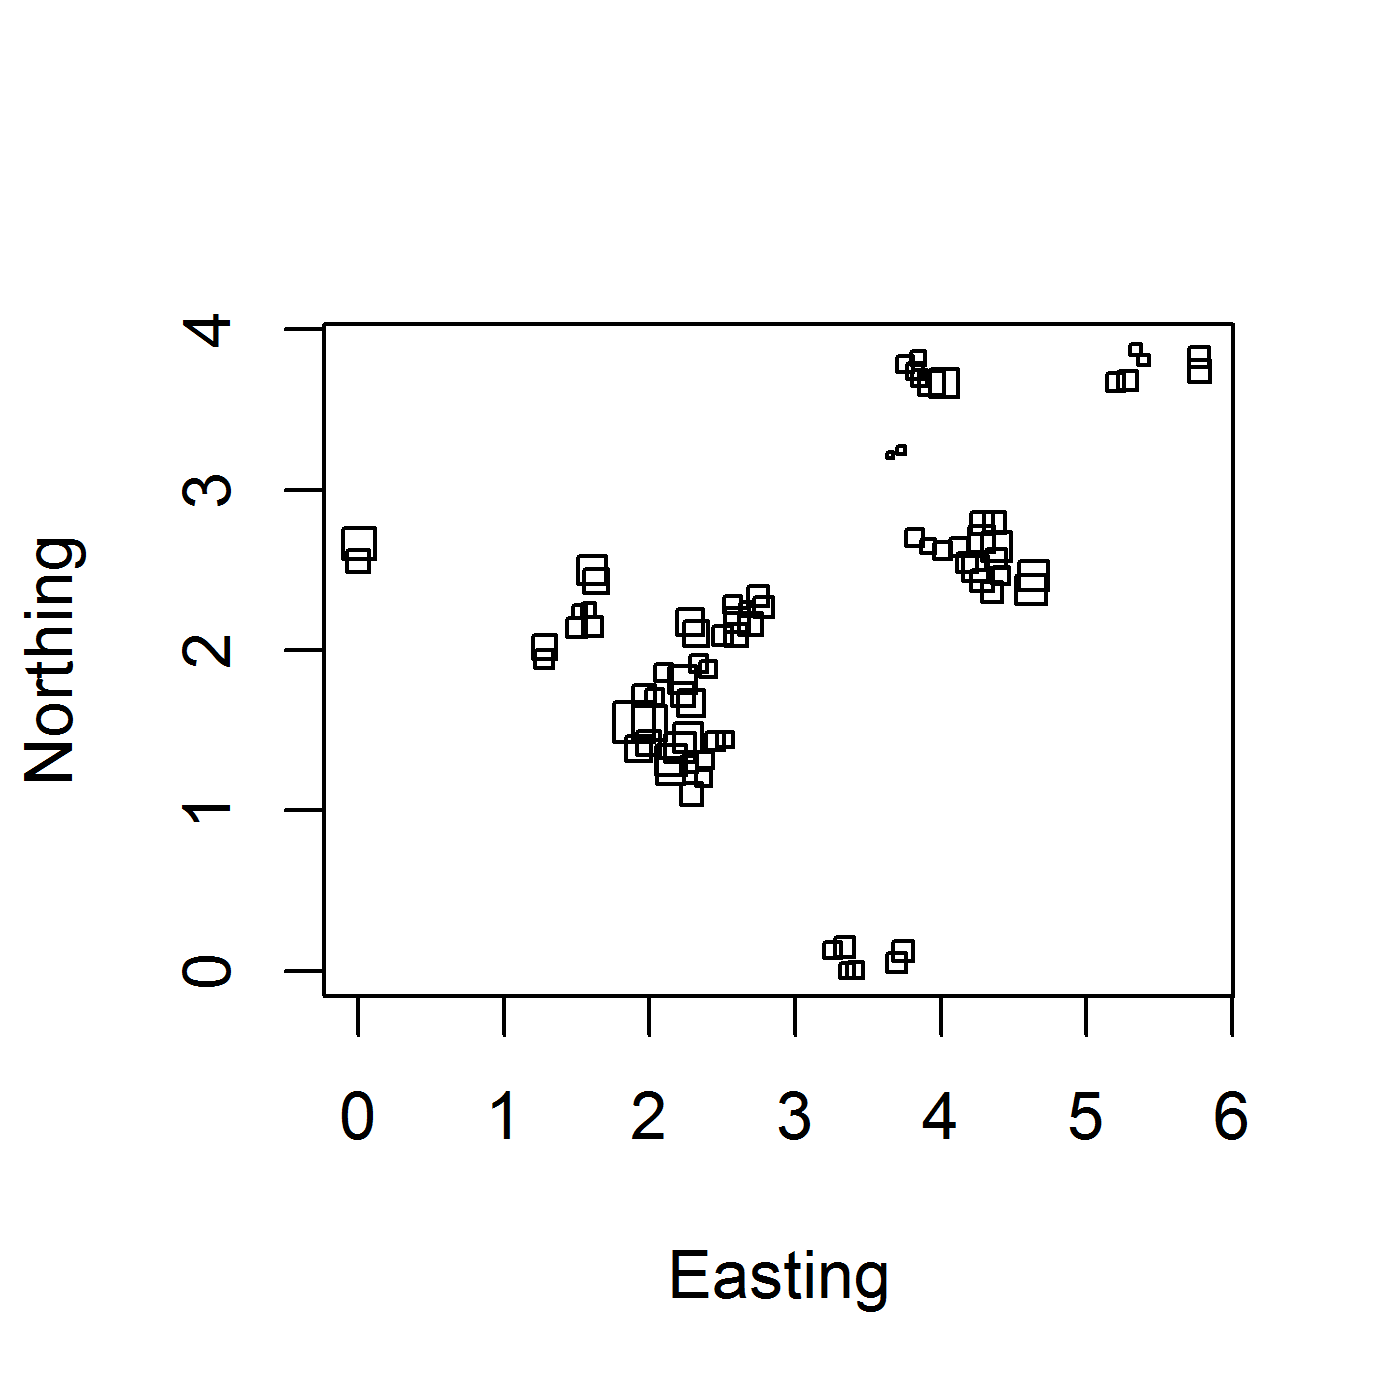
\includegraphics[width=3.5in,height=3.5in]{Ch15-searchencounter/figs/Cap-fragments.png}
\label{poisson-mn.fig.capfrags}
\caption{Relative size and position of 78 forest fragments sampled for
  capricaillie crap.}
\end{figure}
\end{comment}

\begin{figure}
\centering
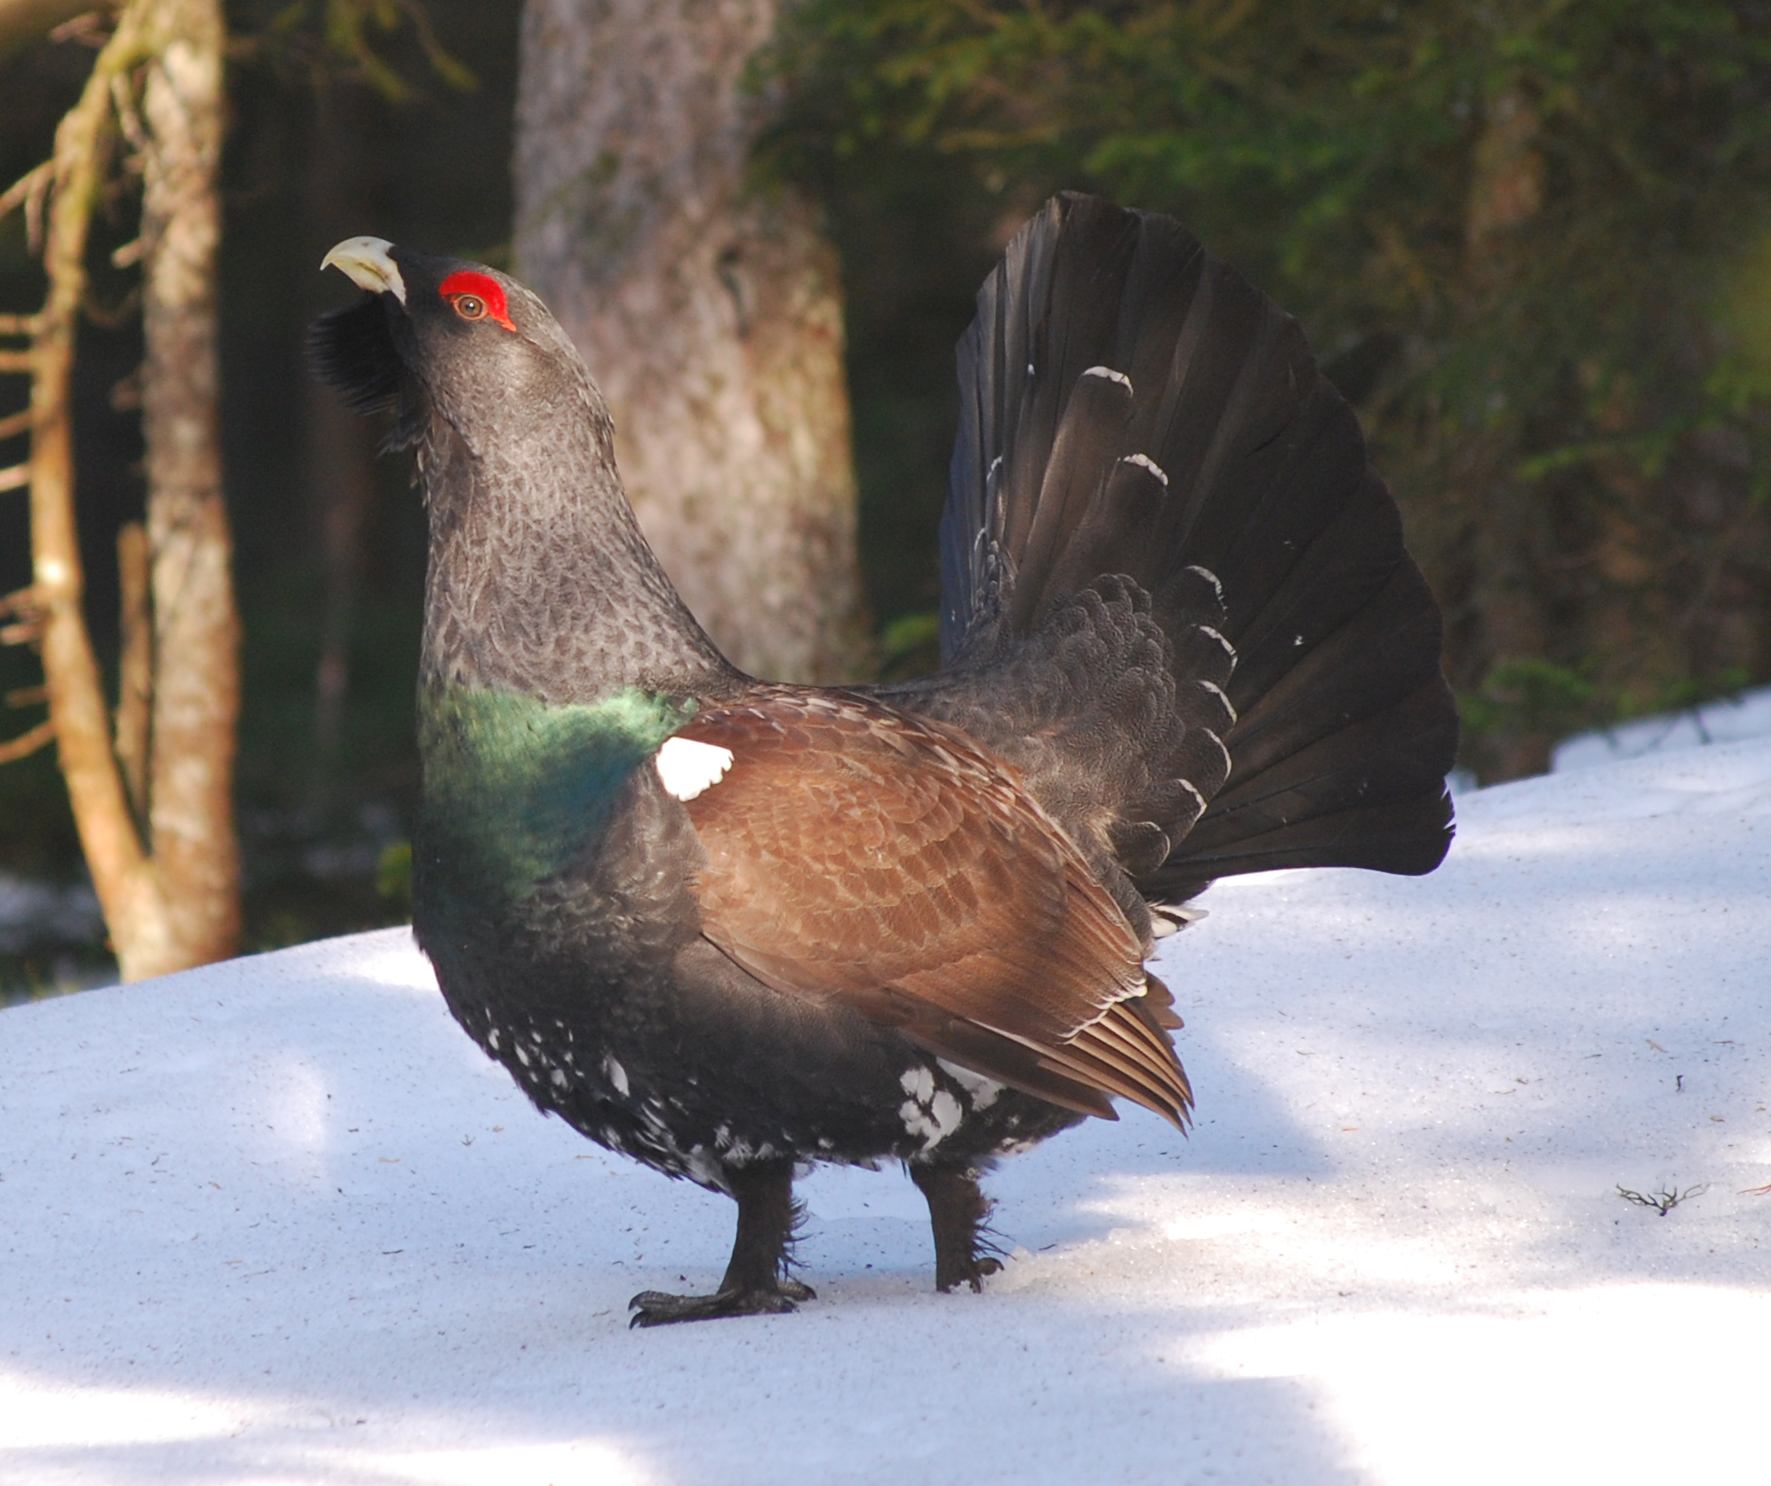
\includegraphics[width=5in,height=4.21in]{Ch15-searchencounter/figs/capercaillie_lanz.jpg}
\label{searchencounter.fig.capercaillie}
\caption{A male caprcaillie in its typical lekking position,
{\it Photo credit: Michael Lanz, Switzerland}.
}
\end{figure}

A key point of the model is that it assumed a discrete model for the
activity centers: activity centers were uniformly distributed to each
of the 78 fragments in proportion to area of the forest patch within
which each fragment was located.  This is similar to the multi-session
formulation of the model where, in this case, the ``sessions'' are
discrete forest fragments but, unlike the multi-session models above,
the encounters of an individual can occur in multiple sessions.  The
authors assumed that
\[
 N_{frag} \sim Poisson( A_{frag} \lambda_{0} )
\]
which implies (see Chapt. \ref{chapt.hscr}):
\[
{\bf s}_{i} \sim  \mbox{Categorical}(  \pi_{frag} )
\]
with
\[
 \pi_{frag} = \frac{ \lambda_{frag} }{\sum_{frag} \lambda_{frag}}
\]
The oservation model: Each of the 78 fragments is its own sample unit which we index to the
center point of the fragment. No finer scale information is made about
the observation locations.
Let $y_{ij}$ be  the number of times individual $i$ encountered in stand $j$.

\subsection{Design 4 -- absence of location information}

We imagine that models can be developed for
situations where we neglect
altogether to record location information within the sample unit.
We see two specific cases here:
Imagine we have a bunch of quadrats or segments that are contiguous or
in close proximity
and we do the surveys like above and record counts PER individual  but
no other sampling information. An example of this is the capericaillie
paper by Mollet et al.....

The other case is that we don't record individual ID at all -- instead
we just have total count frequencies in each plot.
This model is precisely the one considered by
\citep{chandler_royle:2012} and this is the focus of Chapt. \ref{chapt.scr-unmarked}.





\section{Summary and Outlook}

While the use of capture-recapture methods
is commonplace in studies of animal
populations, this includes the classical notion of capture-recapture
based on organized arrays of traps but also a large swath of
``designs'' which are based on organized or haphazard
searches of areas, well-defined or not. For these situations.
Spatial sampling in these ``search-encounter'' situations is distinct
from the classical capture-reapture methods
(e.g., camera trapping) that are based on fixed trap locations.

 In this chapter we showed that SCR models are
relevant to these ``unstructured'' sampling problems in the same way
as ordinary SCR data from trap arrays. One of the key conceptual
points is that, with these search-encounter types of designs, the
locations of observations are {\it not} biased by the locations of
traps but, rather, locations of individuals can occur anywhere within
search plots or quadrats, or in the vicinity of a transect or search
path.  Because we can obtain direct observations of location --
outcomes of movement -- for individuals, it is possible to resolve
explicit models of movement from search-encounter data.  

Key features of what we refer to as ``search-encounter models'' are: 
(1) They contain a model for how space is
sampled, conditional on locations of individuals; and (2) they contain 
a model that
describes how observable animal locations are distributed in space.
We interpret the observable locations as outcomes from a movement
model.  
The models
are somewhat more general than the standard SCR models where
observations are restricted to a priori fixed locations. 

We 
considered the simple case of the independent bivariate normal
movement model, and also a random walk type model, which can easily be
fitted in the {\bf BUGS} engines.  We imagine much more general
movement models can be fitted, although we have had limited
opportunities to pursue this and in most practical capture-recapture
studies, we will probably be limited by sparse data in the complexity
of the movement models that could be consideered. 

We think the search-encounter models will prove to be enormously
useful in future studies of animal populations because so many new
methods of obtaining encounter history data can be be based on DNA
extracted from animal tissue or scat, which is easy to obtain by
searching space and collecting it opportunistically. 


SCR/DS?
%%\chapter{SCR for Search-Encounter Data with Individual Identity}


%\chapter{Open models}
%\label{chapt.open}


%\part{Super-Advanced SCR Models}
%
%\chapter{MCMC chapter}
%\label{chapt.mcmc}

%%\chapter{Spatial Capture-Recapture for Unmarked Populations}
\chapter{Unmarked Populations}
\markboth{Chapter 14 }{}
\label{chapt.scr-unmarked}

\vspace{0.3cm}

%\hl{todo: Royle-Nichols observaiton model}

Traditional capture-recapture models share the fundamental
assumption that each individual in a population can be uniquely
identified when captured. Often, this can be accomplished
by marking individuals with color bands, ear tags, or some other
artifical mark that can be subsequenly read in the field. For other
species, such as tigers (\textit{Panthera tigris}) or
marbled salamanders (\textit{Ambystoma opacum}),
individuals can be easily identified
using only their natural markings. However, many species
do not possess adequate natural markings and are
difficult to capture, making it impractical to use standard
capture-recapture techniques.

Estimating density when individuals are unmarked can be accomplished
using a variety of alternatives to capture-recapture, such as distance
sampling \citep{buckland_etal:2001} and $N$-mixture models
\citep{royle:2004biom}. These methods, and others, can be
very effective when their assumptions are met, but in cases such as
when it is not possible to obtain accurate distance data, or when
movement complicates the use of fixed-area plots,
these methods may not yield unbiased estimates of density
\citep{chandler_etal:2011}. In this chapter we highlight the work of
\citet{chandler_royle:2012} who demonstrated that the ``individual
recognition'' assumption of traditional capture-recapture models is not a
requirement of spatial capture-recapture models. They showed that,
under certain conditions described below, spatially-correlated count
data are sufficient for making inference about animal distribution and
density even when no individuals are marked.
The \citet{chandler_royle:2012} ``spatial count model'' (hereafter the SC
model) requires neither distance data nor fixed area plots. Instead,
the observed data are trap- and occasion-specific counts, which
are modeled as a reduced-information summary of the \textit{latent}
encounter histories. Because the model is formulated in terms of the
data we wish we had, i.e. the typical encounter history data observed
in standard capture-recapture studies of marked animals, the SC model
is just a SCR model with a single extension to account for the fact
that the encounter history data are unobserved.
%To be more precise, we model the counts as:
%$n_{jk} = \sum_i y_{ijk}$ where $n_{jk}$ is the count data and
%$y_{ijk}$ is the encounter history data. Thus, the model
%is virtually identical to standard SCR models except that the
%encounter histories $\{y_{ijk}\}$ are not directly observed.

The ability to fit SCR models to data from unmarked populations has
important implications. For one, it means that SCR models can
be applied to data collected using methods like points counts in which
observers record simple counts of animals at an array of survey
locations. The model can also be fit to camera trapping data collected on
unmarked animals, representing the first formal method for estimating
% XXXX Mention gas model?
%and prior to the SC models
%there were few, if any, options for modeling
density from such data.
So, is this model a free lunch? At face value, it sounds as though it
allows for estimation of
%can estimate
all the quantities of interest in standard
capture-repature studies, but with very little
data. But of course the answer is no --
%The answer is of course not---
lunch is still not free because
with this model come new assumptions,
%which we will describe in this chapter,
and as was demonstrated by
\citet{chandler_royle:2012}, even with ``perfect'' data, the estimates
will typically not be very precise. % as might be hoped for.
This should
not be surprising given that we are asking so much from simple count
data.

The real value of the SC model is two-fold. First, it demonstrates
an important theoretical result, namely
that spatial correlation in
count data carries information about the distribution of
individuals. This stands in stark contrast to a prevailing view of
spatial correlation as a nuisance to be avoided or modeled out of unsightly
residual plots. The second reason why this model is important is that
it provides the basis for handling the extremely common phenomenon in
which only a subset of individuals in a population can be marked or otherwise
distinguishable. Thus, while we do not recommend foregoing the work
required to mark animals, this model does provide a method for
studying unmarked populations, which \textit{can} yield precise
density estimates if some of the individuals are marked, or if prior
information about some of the parameters is available.
The extension of this model to handle data from marked and unmarked
individuals is thoroughly treated in the next chapter. Here, we focus
on the case in which all individuals are unmarked.

\section{Existing Models for Inference About Density in Unmarked Populations}
\label{Sect.existing-unmarked}

When capture-recapture methods are not a viable option, ecologists
often collect simple count data or even binary detection/non-detection data
to estimate parameters such abundance or occupancy.
%\citep{royle:2004biom, mackenzie_etal:2002}.
These
data may be analyzed using generalized linear models such as
Poisson regression or logistic regression, perhaps with random
effects. %When detection is imperfect, as it almost always is,
However, these methods will be biased when detection is imperfect, as
it usually is. Even when count data or detection/non-detection data are
used as an index of abundance or occurrence, standard models may yield
unreliable results when covariates affect both the ecological process
and the observation process. A classic example is given by
\citet{bibby_buckland:1987} who found that songbird detection
probability was negatively related to vegetation height, whereas
density was positively associated with vegetation height in restocked
confier plantations. This intuitive phenomenon has been
demonstrated repeatedly \citep[e.g.][]{kery:2008,sillett_etal:2012} and has led to the
development of a vast number of models to estimate population size and
detection probability when individuals are unmarked. A review of these
models is beyond the scope of this
chapter, but we mention a few deficiencies of existing methods
that warrant the exploration of alternatives for robust inference when
standard capture-recapture methods do not apply.

Distance sampling \citep{buckland_etal:2001}, which we briefly
introduced in Chapter~\ref{chapt.intro},
is perhaps the most widely used method for
estimating population density when individuals are unmarked and
detection probability is less than one. This class of methods is known
to work impecibly when estimating the number of stakes in a field or
the number of duck nests in a wetland. Distance sampling can also work very well in
more interesting situations, and it is an extremely powerful method when
the assumptions can be met. However, the assumptions that distance
data can be recorded without error and that animals are distributed
randomly with respect to the transect can be easily violated by
common processes such as animal movement and measurement
error. Although numerous methods have been proposed to
relax some of these assumptions
\citet{royle_etal:2004, borchers_etal:1998, johnson_etal:2010,
  chandler_etal:2011},
another issue is that distance
sampling is simply not practical in many settings. For example, many
species are so rare and elusive that they can only be reliably
surveyed using methods such as camera traps or hair snares. %, and
%studies employing these techniques are growing in

Other common sampling methods used to estimate density when individuals are
unmarked include double-observer sampling, removal sampling, and
repeated counts, for which custom models have been developed
\citep{nichols_etal:2000, farnsworth_etal:2002, royle:2004biom,
  royle:2004abc, nichols_etal:2009,fiske_chandler:2011}. To
obtain reliable density estimates using these
methods, the area surveyed must be well defined and closed with
respect to movement and demographic processes. Given a sufficiently short
sampling interval, such as a 5-min point-count, the closure
assumption may be reasonable. However, short sampling intervals limit
the number of detections, so observers generally visit each survey
location multiple times during a season. But then, animal
movement may invalidate the closure assumption, and a model of
temporary emigration is required
\citep{kendall_etal:1997,chandler_etal:2011}. Furthermore,
distance-related heterogenity in detection probability can introduce
bias in these models, although this bias is negligible when the
ratio of plot size to the scale parameter of the detection function is low
\citep{efford_dawson:2009}.

We mention these issues not to suggest that existing models do not
have value -- indeed we believe that they can be used to obtain
reliable density estimates in many situations -- rather, our aim is to
highlight the need for alternative methods when the assumptions of
existing methods cannot be met and when spatially-explicit inference
is the objective. %Additionally, the spatial count model
%we discuss in this chapter serves as the foundation for a broad class
%of SCR models in which all or some of the individuals cannot be
%uniquely identified, which is the focus of the next chapter.


\section{Spatial Correlation as Information}
\label{sect.corr-info}

All of the previous methods require some sort of auxiliary information
to model both abundance and detection. For instance, %we might need
multiple observers or distance data or repeated visits
may be required
to ensure
that model parameters are identifiable (but see
  \citep{lele_etal:2012, solymos_etal:2012}). The same is true for
the SC model, but the auxiliary information comes in the form of spatial
correlation, which requires no extra effort to collect
\citep{chandler_royle:2012}. %In fact, it's probably safe to say that
%it is harder to avoid spatial correlation that it is to

It is natural to be suspicious of the claim that spatial correlation
is a good thing. Indeed, elaborate methods have been devised to deal
with spatial correlation as a nuisance parameter
\citep{lichstein_etal:2002,dormann_etal:2007}, and ecologists have been admonisted for
failing to obtain ``real'' replicates uncontaminated by spatial
correlation \citep{hurlbert:1984}. The following heuristic may be
helpful for seeing the value of spatial correlation.

Imagine a 10$\times$10 grid of camera traps and a single unmarked
individual exposed to ``capture'' whose home range center lies in the center of the
trapping grid. If the individual has a small home range size relative
to the extent of the trapping grid, we can imagine what the
spatial correlation structure of the encounters might look
like. If the animal's home range is symmetric around the activity center
then the number of times the individual is detected at each
trap (the trap count) is a function of the distance between the home
range center and the trap; i.e., traps with the same distance
from the activity center will yield counts that are more highly
correlated with one another than traps located at different distances
from the activity center. Thus, the correlation in counts tells us
something about the location of the activity center. It is relatively
intuitive that spatial correlation carries information about
distribution, but what about density?


Imagine now that there are two activity centers located in the traping
grid. Using trap counts alone, %which allow for imperfect detection,
is it possible to determine the number and location of these activity
centers? The answer is yes, at least under certain circumstances.
Figure~\ref{chapt-unmarked.fig.heur} %illustrates the process. The
%figure
shows the locations of the two hypothetical activity centers, and the total
counts made at each trap after 10 survey occasions.
%distance between the sampling location and the individual.
Assuming that animals have bivariate normal home
ranges, the fact that there are two areas in the map with high counts
that dissipate with distance suggests that the most likely number of
individuals given these data is 2. Furthermore, the degree to which
the counts dissipate from the two areas of highest intensity is
information about the home range size parameter $\sigma$. These two
piecies of information are enough to estimate the number of
individuals exposed to sampling -- again, given
that a bivariate normal home range is a valid assumption. Of course,
the data could just as well have been generated by a single individual
whose home range is distinctly biomodal, and thus \textit{as always}
the assumptions of our model need to be carefully examined using our
biological knowledge of the system.

\begin{figure}%[ht!]
\centering
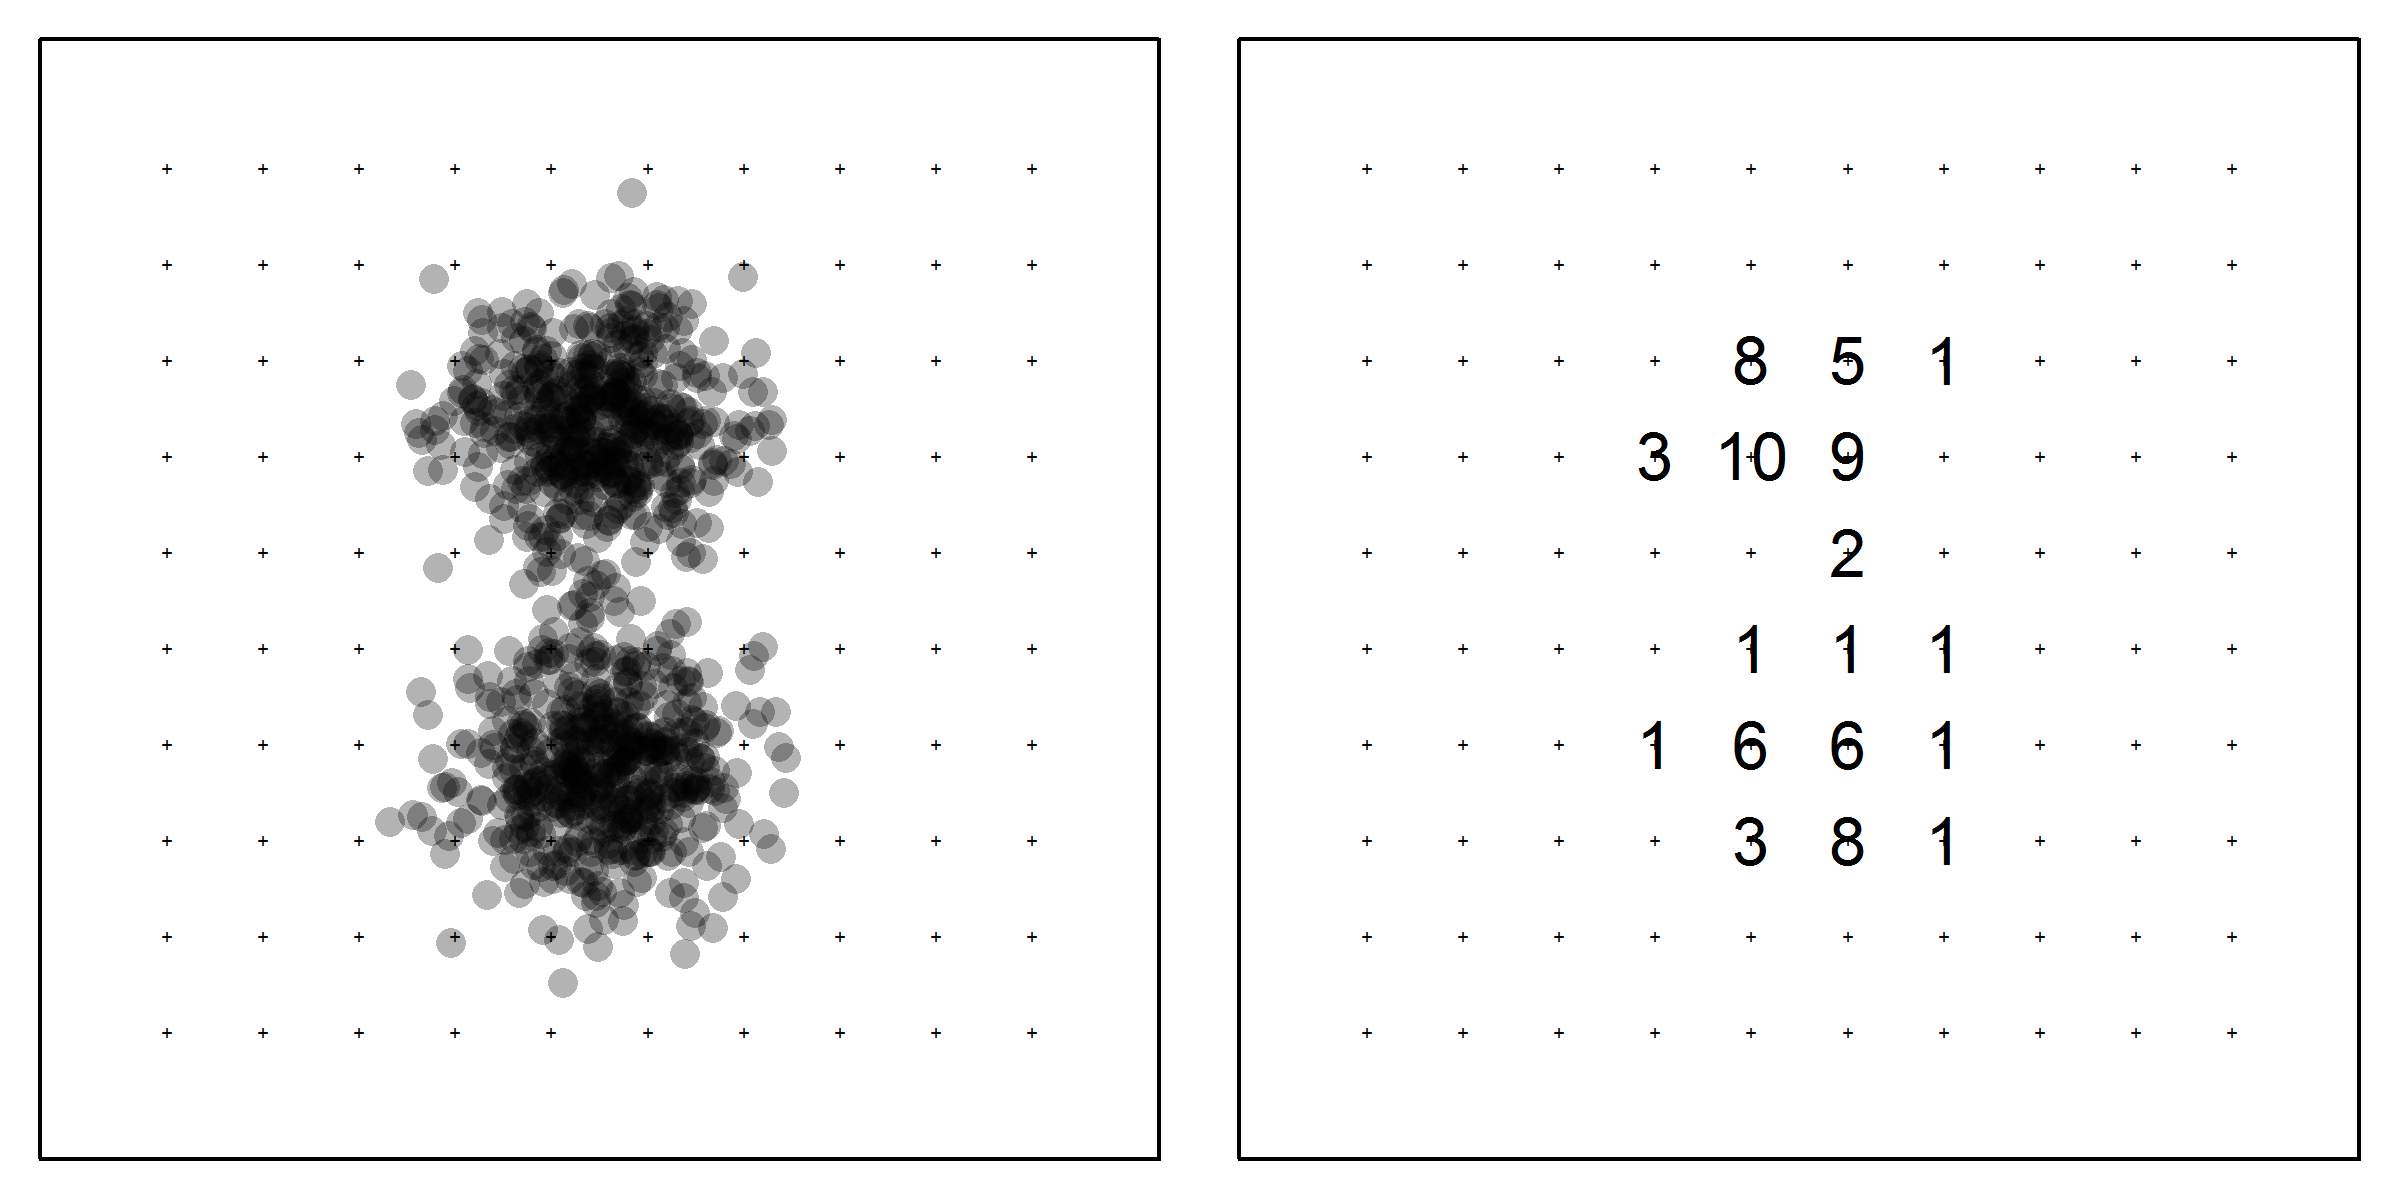
\includegraphics[width=0.5\textwidth]{Ch18-Unmarked/figs/heuristic}
\caption{Simulated count data at each of 100 camera traps
  (crosses) after $K=10$ sampling occasions. The circles are the
  locations of two animal activity centers. The
  \citet{chandler_royle:2012} model estimates %attempts to estimate
  both the location and number of activity centers exposed to
  sampling using such spatially-referenced count data.}
\label{chapt-unmarked.fig.heur}
\end{figure}





\section{Data}

Whereas traditional SCR models require spatially-referenced
encounter histories, this model requires simple count data.
Let $n_{jk}$ be the count data at sampling location $j$ %;
%j=1,\ldots J$
on occasion $k$. %; k=1,\ldots,K$.
The $J \times K$ matrix of
counts will be denoted $\bf{n}$. A sampling location in this context
could be any device capable of recording count data, such as a
human observer or a camera trap, and
one of the benefits of the SC model is that it
can be applied to data collected using many different survey
methods. For ease of presentation, we will refer to sampling devices
as traps, but remember that a trap is just something capable of
recording count data. As in all SCR models, we also require the
coordinates of the $J$ traps, and we denote the location of trap $j$
by ${\bf x}_j$. In some instances, additional data might be avialable such as
trap-specific covariates, state-space covariates,
information on the identities of a subset of individuals, or perhaps
even distance data, but in this chapter we ignore these %extraneous
possibilities so that we can focus on the basic model.

%The duration of sampling
%is assumed to be short enough such that the number of individuals
%exposed to sampling does not change over time.

\section{Model}

The state model is exactly the same as the one we have dealt with
throughout
this book. It is a point process describing the number and distribution of
activity centers in the state-space $\mathcal{S}$. Although it might
be possible to fit inhomogeneous point process models using the
methods described in Chapt.~\ref{chapt.state-space},
%we suspect thatpower to detect effects
given the simplicity of the data, we concentrate on a homogeneous point process
$\{{\bf s}_i, \ldots, {\bf s}_N\} \sim \text{Uniform}(\mathcal{S})$
where ${\bf s}_i$ is the activity center of individual $i$ in the
population of size $N$. For the moment, we will assume that $N$ is
known.

The observation model is the same as in other SCR models %covered
in the sense that it describes the probability of encountering individual
$i$ at trap $j$, conditional on the location of the individual's
activity center. The specific encounter process will depend on the
sampling method, and here we consider the standard camera trapping
situation in which an individual can be encountered at multiple traps
during a single time period, say one night during a camera-trapping
study, and it can be detected multiple times at a single trap during
an occasion. This is the Poisson encounter model (a.k.a. the proximity
detector case) described in
Chapt.~\ref{chapt.poisson-mn}. As before, we define $y_{ijk}$ as the
encounter data for individual $i$ at trap $j$ on occasion $k$, which
we model as:
\begin{equation}
 y_{ijk} \sim \mbox{Poisson}(\lambda_{ij})
\label{eq.latentPoisson}
\end{equation}
where $\lambda_{ij}$ is the encounter rate. A common encounter rate model is the
Gaussian, or half-normal, model:
\[
\lambda_{ij} = \lambda_0 \exp(\| {\bf x}_j - {\bf s}_i \| / 2\sigma^2)
\]
in which $\lambda_0$ is the baseline encounter rate,
$\| {\bf x}_j - {\bf s}_i
\|$ is the Euclidean distance between the trap and activity center, and $\sigma$ is the
scale parameter determining the degree to which encounter rate decreases with
distance.

When individuals cannot be uniquely identified, the encounter histories cannot
be directly observed, which seems like a massively insurmountable
problem. The solution of \citet{chandler_royle:2012} is the same one we routinely apply when we
cannot directly observe the process of interest -- we regard the
encounter histories as latent variables. This leaves the remaining
task of specifying the relationship between the count data and
the encounter histories, i.e. we need a model of $[{\bf n}|{\bf y}]$
where $\bf y$ represents the entire collection of encounter
histories. In this case, there is only one possibility because, by
definition, the count data are simply a
reduced-information summary of the latent encounter histories. That
is, they are the sample- and trap-specific totals, aggregated over all
individuals:
\begin{equation}
n_{jk} = \sum_{i=1}^{N} y_{ijk}.
\label{unmarked.eq.ny}
\end{equation}
So, unlike most model-development problems faced in this book, we
don't have to consider competing probability models for
$[{\bf n}|{\bf y}]$, but instead, we honor the fact that the
relationship between the counts and the latent encounter histories is
deterministic. %You might think that extending the basic SCR model to
%include an additional deterministic component would not be too
%challenging...

%This data structure, a matrix of counts made at a collection of
%sampling locations on one or more occasions is extremely common in
%ecology. For example, think of avian point count data or camera
%trapping data from studies of unmarked animals.

Recall from Chapt.~\ref{chapt.modeling} that the sum of two or more
Poisson random variables is also a Poisson random variable.
Specifically,
if $x_1 \sim \text{Poisson}(\lambda_1)$ and
$x_2 \sim \text{Poisson}(\lambda_2)$, then $(x_1+x_2) \sim
\text{Poisson}(\lambda_1 + \lambda_2)$. Thus,
under this Poisson model for the latent encounter histories,
the count data can be modeled as Poisson:
\begin{equation}
n_{jk} \sim \mbox{Poisson}( \Lambda_{j} )
\label{eq:nagg}
\end{equation}
where
\[
 \Lambda_{j} = \lambda_0 \sum_{i} \exp(\| {\bf x}_j - {\bf s}_i \| / 2\sigma^2),
\]
and because $\Lambda_j$ does not depend on $k$, we can
aggregate the replicated counts, defining
$n_{j.} = \sum_{k} n_{jk}$ and then
\[
 n_{j.} \sim \mbox{Poisson}( K \Lambda_{j} ).
\]
As such, $K$ and $\lambda_{0}$ serve equivalent roles as affecting
baseline encounter rate.
Furthermore, formulating the model in terms of the aggregated count data
demonstrates that the model can be
applied to data from a single sampling occassion $J \equiv 1$, as has
been noted elsewhere for standard SCR models
\citep{efford_etal:2009ecol}. In the context of studying marked
populations, the model parameters will only be identifiable in the
$J\equiv 1$ case if an animal can be captured at multiple traps during
a single occasion. The SC model essentially requires the same thing,
which is to say that it requires correlation in the count data
resulting from an individual being captured in multiple,
closely-spaced traps.

This formulation of the model in terms of the aggregate count also
simplifies computations as the latent encounter histories
do not need to be updated in the MCMC estimation
scheme; however, retaining them in the formulation of the model
is important if some individuals are uniquely marked. %(Chapt.~\ref{chapt.partialID}).
This is because
uniquely identifiable individuals produce
observations of some of the $y_{ijk}$ variables, which we elaborate
on in the subsequent chapter.



\subsection{On $N$ being unknown}
\label{unmarked.sec.N}

Population size, $N$, is never known in practice, and thus %to estimate it,
we need a model for it. For homogeneous point process models,
$N$ is typically modeled as
$N \sim \text{Poisson}(\mu|\mathcal{S}|)$ or
$N \sim \text{Binomial}(M, \psi)$, the latter of which is equivalent
to a discrete uniform prior if $\psi \sim \text{Unif}(0,1)$. In
Chapt.~\ref{chapt.state-space} and elsewhere, we demonstrated that
the choice of prior has very little influence on parameter estimates,
and so we favor the binomial prior because of its convienence when
using MCMC, i.e. it allows us to fix the
dimensions of the parameter space by setting $M$ to some arbitrarily
large integer.

A binomial model is
equivalent to a series of $M$ independent Bernoulli trials, hence
we can rewrite $N \sim \text{Binomial}(M, \psi)$ as $z_i \sim
\text{Bernoulli}(\psi)$ where $z_i$ is an auxilliary variable
indicicating if individual $i$ is a member of the population, i.e. $N =
\sum_{i=1}^M z_i$. Having expanded the model to include a prior on $N$, we
can summarize the SC model, with a Gaussian observation model, as follows:
\begin{align*}
  z_i &\sim \text{Bern}(\psi) \\
  y_{ijk} &\sim \text{Poisson}(\lambda_{ijk} z_i) \\
  \lambda_{ijk} &= \lambda_0\exp(-\|{\bf x}_j - {\bf s}_i\|^2)/(2\sigma^2) \\
  n_{jk} &= \sum_{i=1}^M y_{ijk} %\\
%  N &= \sum_{i=1}^M z_i
\end{align*}

%We note that there are actually two forms of data augmentation going
%on here: (1) we have our usual $M$ instead of $N$ model, and (2) from
%the perspective of modeling count data, we have augmented the model
%with


%\subsection{Inference}

Bayesian analysis can proceed once suitable priors have been put on
the hyperparamters $\psi$, $\sigma$, and
$\lambda_0$. \citet{chandler_royle:2012} provided \R~code for fitting
the model using MCMC, and they evaluated the model's performance with
uniform priors on the three hyperparameters. They also discussed the
possibilities and effects of including prior knowledge about $\sigma$
into the model. In the next section, we explain how the model can be
fit using \jags, but first we briefly contemplate the viability of classical
analysis of this model.

The obvious challenge faced when conducting a classical analysis of
this model is that the number of latent variables in huge. In all SCR models, the activity centers are
latent, but now even the encounter histories are latent.
Maximizing likelihoods with latent variables (random effects) involves
integrating (or summing) over all possible values of the latent
variables. For the activity centers, this is typically accomplished by
integrating the conditional-on-$\bf s$ likelihood $[{\bf y}_i|{\bf s}_i]$ over the two-dimensional
state-space $\mathcal{S}$ (Chapt.~\ref{chapt.mle}). However, with
the SC model, we have to sum
over all possible encounter histories %$\mathcal{H}$
meeting the
constraint of Eq.~\ref{unmarked.eq.ny}. The
number of possible encounter histories
%that could give rise to the count data
will, in general, be too high to make the likelihood tractible,
and thus we do not think that maximum likelihood is a viable option
for analyzing this model. However, one might be able to obtain maximum
likelihood estimates using simulation-based methods
%\citep{doucet_etal:2002,lele_etal:2010},
\citep{lele_etal:2010},
which will typically be more computationally
challenging than the MCMC-based Bayesian analysis.


\section{Simulation Example}

Simulating data under the SC model proceeds by first simulating
standard SCR encounter history data and then collapsing it into count
data. The following blocks of \R~code generate data from
the model shown in Sec.~\ref{unmarked.sec.N}, with parameters
$\sigma=0.04$, $\lambda_0=0.3$, and $N=50$. The state-space is the unit
square and a grid of 100 traps
is centered in the middle. These simulated data might resemble actual
data from a camera trap study in which an individual can be detected multiple
times at a trap during a single occasion, and at multiple traps during
an occasion. The first block of code generates the trap coordinates
$X$ and the $N=50$ activity centers:
\begin{verbatim}
> tr <- seq(0.3, 0.7, length=10)
> X <- cbind(rep(tr, each=length(tr)),
+            rep(tr, times=length(tr)))    # trap coords
> set.seed(10)
> xlim <- c(0, 1); ylim <- c(0, 1)         # S is the unit square
> A <- (xlim[2]-xlim[1])*(ylim[2]-ylim[1]) # area of S
> mu <- 50                                 # density (animals/unit area)
> (N <- rpois(1, mu*A))                    # Generate N=50 as Poisson deviate
[1] 50
> s <- cbind(runif(N, xlim[1], xlim[2]), runif(N, ylim[1], ylim[2]))
> plot(X, xlim=xlim, ylim=ylim, pch="+")
> points(s, col=gray(0.5), pch=16)
\end{verbatim}
We could have set $N=50$ directly, but instead we treated density
as a fixed parameter ($\mu=50$) and generated $N$ as a random
variable -- it just so happens that with the specified random seed,
$N$ equals 50! % Once again, this highlights that fact that $N$ can be
% regarded as either a fixed or a random variable.

Now we can generate the encounter histories under the
Poisson observation model. Let's suppose that sampling is conducted
over $K=5$ nights.
\begin{verbatim}
> sigma <- 0.1
> lam0 <- 0.5
> J <- nrow(X)
> K <- 5
> y <- array(NA, c(N, J, K))
> for(j in 1:J) {
+     dist <- sqrt((X[j,1]-s[,1])^2 + (X[j,2] - s[,2])^2)
+     lambda <- lam0*exp(-dist^2/(2*sigma^2))
+     for(k in 1:K) {
+         y[,j,k] <- rpois(N, lambda)
+     }
+ }
\end{verbatim}

The object \verb+y+ is the $N \times J \times K$ array of encounter
data, which cannot be directly observed if the animals are unmarked.
Converting the encounter data to count data can be accomplished using a single
\verb+apply+ command.
\begin{small}
\begin{verbatim}
> n <- apply(y, c(2,3), sum)
> dimnames(n) <- list(paste("trap", 1:J, sep=""),
+                     paste("night", 1:K, sep=""))
> n[1:4,]
      night1 night2 night3 night4 night5
trap1      0      0      0      0      0
trap2      1      0      0      2      1
trap3      0      0      1      2      0
trap4      2      0      1      0      1
\end{verbatim}
\end{small}
This object \verb+n+ is the $J \times K$ matrix of counts that we call
$\bf n$. It is worth comtemplaing how common such count data is in
ecology and how many different mechanisms might generate it. Although
the list of possibilites is immense, the SC model has advantages over
some alternatives
%approximation to reality in many cases
in that it includes an explicit
model for the distribution of individuals in space \textit{and} it
includes a model describing how detections are generated given the
distance between traps and individual activity centers. It also
provides a foundation for extending the model in many ways as we
discuss in Sec.~\ref{unmarked.ext} and in the next chapter.

The question now is: Is it possible to estimate the parameters? In our
simulated dataset we have $J \times K = 500$ data points, but how many
parameters do we need to estimate with this rather small set of data?
A frequentist might say that there are only 3 parameters: $\lambda_0$,
$\sigma$, and $N$ (or density $\mu$) because inference about the
latent parameters is carried out using prediction methods after the 3
hyperparameters have been estimated. However, a Bayesian would
probably say that each $\bf s$ and each element of the latent
encounter array $\bf y$ is a parameter in need of a posterior. From
this perspective there are far more parameters than data points, and
thus it would appear as though the situation is dire. Whether or not
the parameters are actually estimable is a rather difficult question
to answer. One simplistic, but not definitive, approach for addressing
the question is to conduct a simulation study and evaluate the
frequentist performance of the model by asking how often the
data-generating values are included in confidence/credible intervals,
and how biased are point estimates. \citet{chandler_royle:2012}
conducted such a simulation study and found that, while the variance
of the posterior distributions was high by most standards, the bias of
the posterior mode of $N$ was small and the coverage of the credible
intervals was close to nominal. Moreover, they found no evidence that the
posterior distributions were dominated by the priors, further
supporting the conclusion that spatial correlation in the count data
is sufficient for estimating density and encounter probability
parameters. %Rather than repeating their simulation study, we present
%a few options for fitting the model.

At this point in time the SC model can only be fit using one of the
\bugs~engines, or using custom software like the \R~code accompanying
\citet{chandler_royle:2012}. Although \bugs~might provide the most
flexible option for fitting the model, it is not
straight-forward because of the
constraints in the model. In \textbf{WinBUGS}, the contraints can be
enforced using the so-called ``ones-trick'', but we prefer
\jags~because it has a distribution
called \verb+dsum+ that was designed for this type
of situation where the observed data are a sum of random
variables. %Aside from being slow, \jags~works rather well for this
%situation. %Another limitation of using \jags~is that
%we can't mix data from marked and unmarked individuals because
%\verb+dsum+ requires that we sum over unobserved quantities, not a mix
%of observed and unobserved nodes. Thus, we can't use \jags~for the
%situations considered in the next chapter, and thus we wrote our own
%MCMC algorithm which overcomes these limitations, and it is somewhat
%faster. Nonetheless,
Panel~\ref{unmarked.panel.jags1} shows an implementation in \jags.
Note that this code will not run as shown because we abbreviated the
arguments to \verb+dsum+. In practice, you need to provide all $M$ of
them, where $M \gg N$ is the size of augmented latent encounter
array. The code looks slightly unwieldy if $M$ is large, but you can easily create
it using the \verb+paste+ function in \R. Here is an example, with an
unrealistically small value of $M=10$:
\begin{small}
\begin{verbatim}
> paste("y[", 1:10, ",j,k]", sep="", collapse=", ")
[1] "y[1,j,k], y[2,j,k], y[3,j,k], y[4,j,k], y[5,j,k], y[6,j,k],
y[7,j,k], y[8,j,k], y[9,j,k], y[10,j,k]"
\end{verbatim}
\end{small}
This output can be pasted directly into a \jags~model file.
%Maybe Martyn Plummer will throw us
%a bone and allow for a vector as an argument. Anyhow,
% XXXX
%The entire analysis is shown on the ???XX help page in \scrbook.

\begin{panel}
\centering
\rule[0.05in]{\textwidth}{.03in}
\begin{small}
\begin{verbatim}
model{
sigma ~ dunif(0, 200) # Tailor this to your state-space
lam0 ~ dunif(0, 5)    # consider dgamma() as an alternative
psi ~ dbeta(1,1)
for(i in 1:M) {
   z[i] ~ dbern(psi)
   s[i,1] ~ dunif(xlim[1], xlim[2])
   s[i,2] ~ dunif(ylim[1], ylim[2])
   for(j in 1:J) { # Number of traps
       distsq[i,j] <- (s[i,1] - X[j,1])^2 + (s[i,2] - X[j,2])^2
       lam[i,j] <- lam0 * exp(-distsq[i,j] / (2*sigma^2))
       for(k in 1:K) { # Number of occasions
           y[i,j,k] ~ dpois(lam[i,j]*z[i])
           }
       }
   }
for(j in 1:J) {
   for(k in 1:K) {
       n[j,k] ~ dsum(y[1,j,k], y[2,j,k], ..., y[200,j,k]) # Code abbreviated!!
       }
   }
N <- sum(z[])   # Realized population size
A <- (xlim[2]-xlim[1])*(ylim[2]-ylim[1]) # Area of state-space
D <- N / A      # Realized density
ED <- (M*psi)/A # Expected density
}

\end{verbatim}
\end{small}
\rule[0.15in]{\textwidth}{.03in}
\caption{\jags~code to fit the spatial count model. This version
  includes the latent encounter histories.}
\label{unmarked.panel.jags1}
\end{panel}

The \jags~model in Panel~\ref{unmarked.panel.jags1} can be used to
fit the version of the model in which the latent encounters are
updated at each Monte Carlo iteration. One challenge faced when using
this version of the model is that \jags~cannot auto-generate initial values
that honor the contraints in the model, so it is necesssary to provide
them. The following code presents one fairly general way of creating
acceptable starting values and formatting the data for analysis using
the \texttt{rjags} package:
\begin{small}
\begin{verbatim}
library(rjags)
dat1 <- list(n=n, X=X, J=J, K=K, M=200, xlim=xlim, ylim=ylim)
init1 <- function() {
    yi <- array(0, c(dat1$M, dat1$J, dat1$K))
    for(j in 1:dat1$J) {
        for(k in 1:dat1$K) {
            yi[sample(1:dat1$M, dat1$n[j,k]),j,k] <- 1
        }
    }
    list(sigma=runif(1, 1, 2), lam0=runif(1),
         y=yi, z=rep(1, dat1$M))
}
pars1 <- c("lam0", "sigma", "N", "mu")
\end{verbatim}
\end{small}
Fitting the model can then be done using the functions
\verb+jags.model+ and \verb+coda.samples+.
%, we use two functions. The first
\verb+jags.model+ compiles the code and runs an adaptive phase to
increase the efficency of the MCMC samplers. The second function
\verb+coda.samples+ is one of several options for generating
posterior samples. We like it because it returns the samples in the
format required by the \texttt{coda} package.

The code in Panel~\ref{unmarked.panel.jags1} %represents the full
%model in which the latent encounter histories are updated at each step
%in the MCMC algorithm. This formulation
is useful because it shows how
closely this model is related to standard SCR models, and it provides
the basis for including data on both marked and unmarked individuals,
as will be discussed in the next chapter. However, this model runs
very slowly, even when using a fast 64-bit machine with chains run in parallel. The code
in Panel~\ref{unmarked.panel.jags2} runs much faster because it
does not include the latent encounter histories. %Here is the code:
%Instead, it fits the model using the

\begin{panel}
\centering
\rule[0.05in]{\textwidth}{.03in}
\begin{small}
\begin{verbatim}
model{
sigma ~ dunif(0, 200)
lam0 ~ dunif(0, 5)
psi ~ dbeta(1,1)
for(i in 1:M) {
   z[i] ~ dbern(psi)
   s[i,1] ~ dunif(xlim[1], xlim[2])
   s[i,2] ~ dunif(ylim[1], ylim[2])
   for(j in 1:J) { # Number of traps
       distsq[i,j] <- (s[i,1] - X[j,1])^2 + (s[i,2] - X[j,2])^2
       lam[i,j] <- lam0 * exp(-distsq[i,j] / (2*sigma^2)) * z[i]
       }
   }
for(j in 1:J) {
   bigLambda[j] <- sum(lam[,j])
   for(k in 1:K) {
       n[j,k] ~ dpois(bigLambda[j])
       }
   }
N <- sum(z[])
A <- (xlim[2]-xlim[1])*(ylim[2]-ylim[1]) * 10000 # Area of state-space (ha)
D <- N / A      # Realized density
ED <- (M*psi)/A # Expected density
}
\end{verbatim}
\end{small}
\rule[0.15in]{\textwidth}{.03in}
\caption{\jags~code to fit the spatial count model. This version
  does not include the latent encounter histories, and thus runs much
  faster than the code in Panel~\ref{unmarked.panel.jags1}.}
\label{unmarked.panel.jags2}
\end{panel}



An even faster alternative is to use the \verb+scrUN+ function in
\texttt{scrbook}, which is a modified version of the code presented in
the Supplement of \citet{chandler_royle:2012}. The usage is as
follows:
\begin{verbatim}
out1 <- scrUN(n=n, X=X, M=250, niter=250000, xlims=xlim, ylims=ylim,
               inits=list(lam0=0.3, sigma=0.01), updateY=TRUE,
               tune=c(0.004, 0.09, 0.35))
\end{verbatim}
where \verb+n+ is the matrix of counts, \verb+X+ is the trap
coordinate matrix, \verb+M+ sets the size of the data-augmented latent
data, \verb+xlims+ and \verb+ylims+ define the
rectangular state-space, \verb+inits+ is a list of starting values,
and \verb+updateY+ determines if the latent encounter histories are
updated as part of the MCMC algorithm. In general, %there is no reason
%to set
we recommend using the option
\verb+updateY=FALSE+ because we find that the Markov chains mix
better. %since it may take longer to run and the
%mixing may be poorer, but we provide both options so that readers can
%look under the MCMC hood and see the basis of the models and code
%presented in the next chapter. Further details about the model
%arguments and output are given on the function's help page.
However, it can be important fiddle with the tuning parameters until the
acceptance rates are between 40--60\%. Otherwise, the Markov chains
will exhibit high autocorrelation.

We used the model with no latent encounter histories using both
\jags~and \verb+scrUN+ to the simulated data, and the results
are given in TableXXXX.








\section{The Northern Parula Study}

Here we re-analyze the northern parula ({\it Parula americana}) data
described in \citet{chandler_royle:2012}. The data were collected at
105 points located on a 50-m grid at the Patuxent Wildlife Research
Center. Each point was surveyed 3 times during June 2006, and
Fig.~\ref{fig:nopaDat} depicts the resulting spatially-correlated
counts ($n_{j.}$). A total of 226 detections were made with a maximum
count of 4 during a single survey. At 38 points, no warblers were
detected. All but one of the detections were of singing males, and
this one observation was not included in the analysis.

\begin{figure}
  \centering
  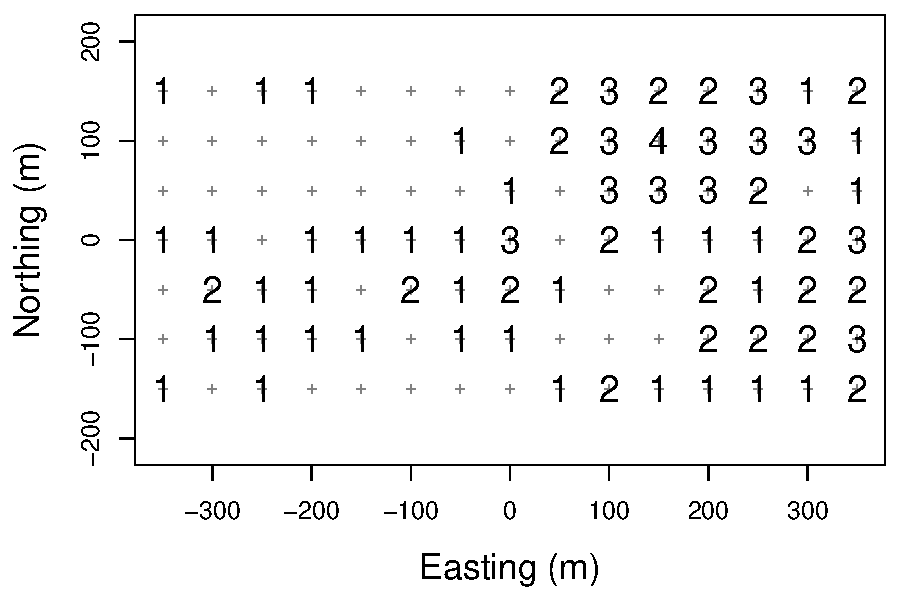
\includegraphics[width=0.8\textwidth]{Ch18-Unmarked/figs/nopaCounts}
  \caption{Spatially-correlated counts of northern parula. Gray
    crosses are the locations of the 105 point count
    stations. Superimposed are the number of detections after 3 survey occasions.}
  \label{fig:nopaDat}
\end{figure}


We used both versions of the code to fit the
model to the parula data. In our analyses, we defined the point process
state-space by buffering the grid of point count locations by 250 m,
and we set $M=200$. For inference, we generated three Markov chains,
each consisting of 300000 iterations after discarding the initial 10000
draws. %Convergence was satisfactory, as indicated by an $\hat{R}$
%statistic of $<$ 1.02 \citep{gelman_rubin:1992}.
\begin{small}
\begin{verbatim}
library(scrbook)
library(rjags)
data(nopa)
dat1 <- list(n = nopa$n, X = nopa$X, M=200, J=nrow(nopa$n), K=ncol(nopa$n),
             xlim=c(-600, 600), ylim=c(-400, 400))
init1 <- function() {
    n <- dat1$n
    J <- nrow(n); K <- ncol(n); M <- dat1$M
    y <- array(0L, c(M, J, K))
    for(j in 1:J) {
        for(k in 1:K) {
            y[sample(1:M, n[j,k]),j,k] <- 1
        }
    }
    list(y = y, sigma=rnorm(1, 100), lam0=0.5, z=rep(1, M))
}
pars1 <- c("sigma", "lam0", "N", "ED")
jm1 <- jags.model("nopa1.jag", dat1, init1, n.chains=3, n.adapt=500)
jc1 <- coda.samples(jm1, pars1, n.iter=31000)
\end{verbatim}
\end{small}




Because these models can take so long to run, we show \R~commands for
fitting the model using a single processor, and code for parallel
processing, which allows us to run 1 chain on each core. Obviously
your computer must have $>1$ core to do this, and you must have a
relatively recent version of \R~so that you can use the {\tt parallel}
package. First, the simple single-core code:




XXXX THE RESULTS OF THE TWO ANALYSES LOOK VERY SIMILAR AS EXPECTED XXXX

The posterior distribution for
$N$ was highly skewed with a long right tail resulting in a wide 95\%
credible interval (Table \ref{t:nopaPosts}). Nonetheless, the interval
for density, $D$, includes estimates reported from more intensive field
studies \citep{moldenhaer_regelski:1996}. As with any SCR model,
we can produce a density surface map, as shown in Fig.~\ref{fig:nopaDen}




We see that, even with simulated data -- data that meets all of the
model assumptions -- the precision of the posterior distributions is
low and mixing is poor. This should be expected given that we are
asking so much from so little data. In essence we are trying to fit a
point process model being twice removed from the actual point
locations. These difficulties may warrant the investigation of simpler
models, but in many cases, the simplificat... Another option is to
figure out ways of improving model precision.


\section{Improving Precision with Prior Information}
\label{Sect.precision}

We are asking a lot of a little data. Because both the activity
centers and the encounter histories are latent variables, there is
inherently high uncertainty in the data, even if it is ``perfect''
data simulated from the true model. This explains the low posterior
precision in the parula data.

So why not just collect distance data or something? If you can, great---
we are not arguing against the use of other methods. But in many
cases, other models are not applicable. For instance, our model could
be applied to camera trapping data collected on species without
natural marks, such as pumas or coyotes. In addition, this
model provides an important foundation for modeling data where other
methods do not apply, and the underlying state model is so damn cool
because it corresponds to what we think is happening in the field.
Furthermore, the potential generalizations are numerous as we
will see later in this chapter and in the next chapter. In sum, the
model can be applied where no other models can, and it provides the
foundation for important extensions, but how can we improve precision?

Indeed, extensive information on home range size has
been compiled for many species in diverse habitats %\emph{e.g.}
\citep[\emph{e.g.},][]{degraaf_yamasaki:2001}. It is
easy to embody this information in a prior distribution as we
demonstrated for the parula data.


One benefit of a Bayesian analysis is that it can accommodate prior
information on the home range size and encounter rate parameters,
which are readily available for many
species. To illustrate, we analyzed the parula data using a new set of
priors. Whereas in the first analysis, all priors were
improper, customary non-informative priors (see Table \ref{t:nopaPosts}),
in the second set we used
an informative prior for the scale parameter $\sigma \sim
\mbox{Gamma}(13,10)$. We arrived at this prior using the methods
described by \citet{royle_etal:2011mee} and published
information on the warbler's home range size and detection probability
\citep{moldenhaer_regelski:1996,simons_etal:2009}. More details on this
derivation are found in ??????. We briefly note here that this prior
includes the biologically-plausible range of values from $\sigma$
suggested by the published literature.


This was true when considering
both sets of priors, although posterior precision was higher under the
informative set of priors. Specifically, the use of prior information
reduced posterior density at high, biologically implausible,
values of $\sigma$, and hence decreased the posterior mass for
low values of $N$ (Fig.~\ref{fig:prior}).






\section{Improving Precision Using Ancillary Data}
\label{unmarked.ext}

%Noting the relatively low precision of the posterior distributions,
\citet{chandler_royle:2012} recommended two strategies for improving
the precision of the posterior distributions obtained under this
model: mark a subset of individuals and/or elicit informative
priors from the published literature. Both of these options should be
feasible in many studies of unmarked populations, but in some cases a
better alternative may be to collect
additional data %in the form of %and here we describe an extension of the model meant
%to accomodate data
such as
distance measurements, % or perhaps %other
%commonly-collected data such as
removal counts, or %perhaps
double observer counts.

In this section, we describe model extensions for accomodating
auxiliary data as a means of increasing posterior precision. Buy why
would we bother with the SC model at all when data
such as distance measurements are available? Isn't density estimable
using the distance data alone? Yes, it is, and in many situations a
simple distance sampling model will be sufficient. However, unlike the
situation we described earlier in this chapter where we viewed spatial
correlation as a good thing, the model extension we describe now
provides a means of dealing with spatial correlation when it is
unwanted or perhaps unavoidable.

As an example, consider the norther parula data analyzed by
\citet{chandler_royle:2012}. These point count locations were spaced
by only 50 m, and since the song of the parula can be easily heard
from a distance of $>100$ m, the neighboring counts exhibit
correlation. As it turns out, the data collected were more than just
the simple counts -- the observers also recorded if each detected
individual was within or beyond 100 m. Although not ideal, distance
data binned into 2 intervals are sufficient for estimating the scale
parameter of a distance sampling detection function, and thus we
should be able to use that information in our expanded model. Doing
so, however, requires that we consider not only the activity centers,
but also the actual locations of individuals during each survey --
much in the same way as is done in search-encounter models
(Chapt.~\ref{chapt.search-encounter}). In fact, the model we are about
to describe is essentially a hybrid SC and search-encounter
model. First, consider another example.

The parula data were
intentionally collected in such a way as to ensure spatial
correlation. This was done
so that the SC model could be evaluated using data other than junk
simulated on our computers. In other cases, spatial correlation occurs
because we need to establish many survey locations in a relatively
small area, and as a result, some individuals may occur at multiple
plots. An example of this is demonstrated in Fig.~\ref{}. These data
are northern dusky salamanders \textit{} in a small stream
network. Rather than sample a few plots in the stream, the entire
stream was surveyed. Actually, several such stream networks were
surveyed in this way, although we will retrict our attention to the
data shown in the figure. This method of sampling makes sense as it
results in many detections and it provides a thorough picture of the
entire stream network.


\begin{figure}
  \centering
  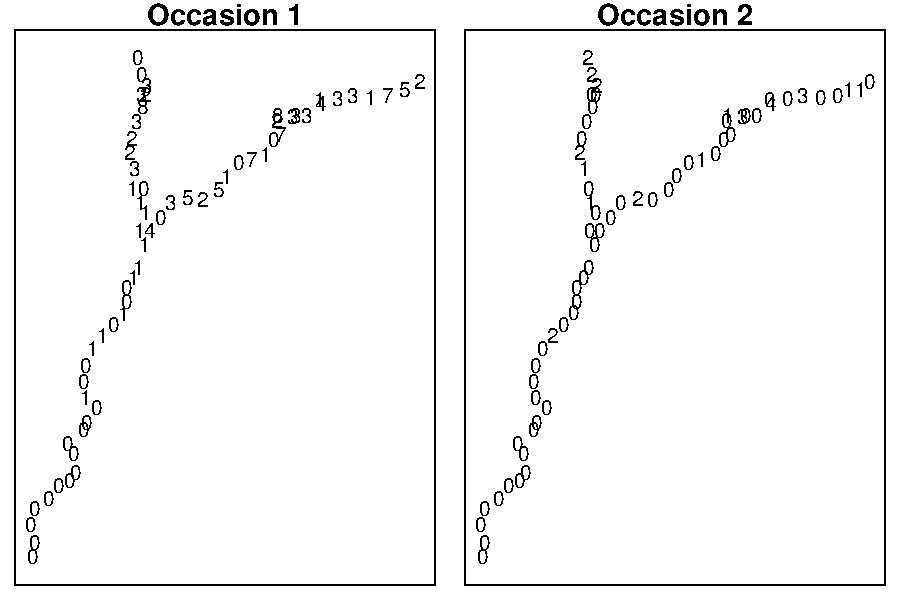
\includegraphics[width=0.8\textwidth]{Ch18-Unmarked/figs/saln27}
  \caption{Stream segment counts of northern dusky salamanders along a
    stream in the Chesapeak and Ohio National Historic Park,
    VA/MD. Each segment is a 50-m stretch in which 3 removal passes
    are made on 3 occasions each summer (only 2 occasions are shown
    here). Notice the consistency of the spatial correlation between
    occasions and the apparent decrease in abundance.}
  \label{unmarked.fig.salct}
\end{figure}




To include data such as the parula distance data or the dusky
salamander removal counts, we need to expand the model to include a
simple movement model. The reason is that the distances are .

Perhaps the simplest model of movement outcomes around the activity
centers is the bivariate normal model
$u_{ijk} \sim Binormal({\bf s}_i, {\bf \Sigma})$.
In this way, we can model the probability of detection given the
distance between a trap and an individual's actual location, instead
of the individual's activity center as we typically do.




\begin{panel}
\centering
\rule[0.05in]{\textwidth}{.03in}
\begin{small}
\begin{verbatim}
model {
p ~ dbeta(1,1)        # detection prob
tau ~ dunif(0, 5000)  # "movement parameter" of Gaussian kernel model
psi ~ dbeta(1,1)      # data augmentation parameter
for(i in 1:M) {
  z[i] ~ dbern(psi)
  s[i] ~ dcat(PrSeg[]) # location (stream segment) of activity center
  for(g in 1:G) {
    PrU[i,g] <- exp(-distmat[s[i],g]^2/(2*tau^2)) # Pr(u | s)
    }
  for(k in 1:K) {
    u[i,k] ~ dcat(PrU[i,]) # location of guy i at time k
    for(g in 1:G) {
      y[i,g,k] <- (u[i,k] == g)*z[i]
      }
    }
  }
for(j in 1:J) {
  for(k in 1:K) {
    N[j,k] <- sum(y[,seg[j],k]) # Number of individuals in seg j at time k
    # removal model:
    n[j,1,k] ~ dbin(p, N[j,k])
    N2[j,k] <- N[j,k] - n[j,1,k]
    n[j,2,k] ~ dbin(p, N2[j,k])
    N3[j,k] <- N2[j,k] - n[j,2,k]
    n[j,3,k] ~ dbin(p, N3[j,k])
    }
  }
Ntot <- sum(z[])
}
\end{verbatim}
\end{small}
\rule[0.05in]{\textwidth}{.03in}
\caption{\bugs~description of model in which ...}
\label{unmarked.panel.sal}
\end{panel}





\subsection{Similarity to other data augmentation schemes}

By including the $w$ variables in the model, we have made use of the
data augmentation technique introduced by \citet{royle_etal:2007} and
developed by \citep{royle:2009} and
\citep{royle_dorazio:2010}. However, including the latent encounter
histories in the model can also be viewed as another form of data
augmentation, which was in fact, first proposed as a general model of
spatial dependence in count data
\citep{wolpert_ickstadt:1998}.

The model of
\citet{wolpert_ickstadt:1998} is slighly different than the SC model
in that they defined $\{{\bf s}_1, \ldots, {\bf s}_N\}$ not as a
realization from a spatial point process, but rather as locations of a
dense array of points, typically a fine grid covering the $J$ survey
locations. The purpose of this grid is to introduce random spatial noise into the system,
which is then smoothed using what, in our case, is the encounter
model. In their case, the encounter model is simply a smoothing
kernel that determines the spatial covariance structure -- if $\sigma$
is high relative to the ``trap'' spacing, the counts will be highly
correlated, and vice versa. Similar ideas have been used to model
spatial dependence in temperature data \citep{higdon:1998}. In the SC
model, $\sigma$ and the encounter model also determine the spatial
correlation, but it has an explicit connection to
correlation as information about the number and location of the
activity centers.

In addition to the fact that they fixed
the locations of the $\bf s$'s, their model also differs from the SC
model in that they also fix $N$, it being chosen to create a suitably
fine grid for generating the white noise.




\section{Design issues}

\subsection{How Much Correlation Is Enough?}

$\sigma$ shouldn't be too small or too large relative to trap spacing.

Can we test for correlation using K-functions or something?

\subsection{Linear Designs}

Survey points are not always located on a grid with even spacing---in
fact, it is rare to see a perfect 10$\times$10 grid of points in any
study because of habitat patchiness or rugged terrain or what have
you. Instead, points are often distributed haphazardly or using some form of
probability sampling. Such designs can still produce data amenable to
the models we consider in this chapter if individuals can be
encountered at multiple points, and none of the considerations
discussed above need to be modified. But what about linear designs?

In bird studies, point counts are often placed on linear transects. For
example, the Breeding Bird Survey involves surveying 50 points spaced
by 0.5 miles. The mountain-top bird survey in the White Mountain
National Forest involves surveying 42 transects, each with 20? points
spaced by 250-m \citep{king_etal:2008}. For many species, the 0.5 mile
spacing of the BBS will ensure that individuals are not detected at
multiple points. However, in the moutain-top survey, it's easy to
imagine that a Bicknell's Thrush (\emph{Catharus bicknelli}) could
easily be heard from adjacent points. So can we apply our model to
obtain density estimates with such simple counts?



%\subsection{Quadrat counts}





\section{Alternative Observation Models}
\label{Sect.alt-obsmods}

\citet{chandler_royle:2012} focused exclusively on the Poisson
observation model, but noted that alternative models such as the
Bernoulli model or the multinomial model (Chapt. \ref{chapt.poisson-mn}) should
be easily accomodated. Unfortunately, our experimentation with these models
indicates that the base-line encounter probability parameter $p_0$ is
not identifiable. At this point in time, it is not clear why this
would be so. However, this situation is similar to that of traditional
mark-resight models where the unmarked individuals provide no
information about the parameters of the capture process. Under these
models, capture or re-sight probability can only be estimated by
marking a subset of the population. In the next chapter we demonstrate
how data from marked and unmarked individuals can be combined to
improve precision and allow for the estimation of parameters under the
alternative observation models.



\subsection{Spatial point process models}


Our model has some direct linkages to existing point process
models. We note that the observation intensity function (i.e.,
corresponding to the observation
locations) is a compound Gaussian kernel similar to
that of the Thomas process
\citep[pp. 61-62]{thomas:1949, moller_waagepetersen:2004}.
Also, the Poisson-Gamma Convolution models
\citep{wolpert_ickstadt:1998} are structurally similar (see also \cite{higdon:1998}
and \cite{best_etal:2000}).
 In particular, our model is such a model but
with a {\it constant} basal encounter rate $\lambda_{0}$
and {\it unknown} number and location of ``support points'', which in
our case are the animal activity centers, $\bf{s_i}$.
We can thus regard our model as a model for
{\it estimating} the location and local density of support points in
such models, which we believe could be useful in the application of
convolution models.  \citet{best_etal:2000} devise an MCMC algorithm for the
Poisson-Gamma model based on data augmentation, which is
similar to the component of our algorithm for
updating the $z$ variables in
the conditional-on-$z$ formulation of the model.  We emphasize that
our model is distinct from these Poisson-Gamma models
in that the number {\it and} location of such
support points are estimated.


If individuals were perfectly observable then the resulting point
process of locations is clearly a standard Poisson or Binomial (fixed
$N$) cluster process or Neyman-Scott process.
If detection is uniform over space but
imperfect, then the basic process is unaffected by this random thinning.
Our model can therefore be viewed formally as a Poisson (or Binomial)
cluster process model but one in which the thinning is
non-uniform, governed by the encounter model which dictates that
thinning rate increases with distance from the observation points. In
addition, our inference objective is, essentially, to estimate the
number of parents in the underlying Poisson cluster
process,
where the observations are biased by an incomplete sampling apparatus
(points in space).


As a model of a thinned point process, our model has much in common
with classical distance sampling models \citep{buckland_etal:2001}.
The main distinction is that our data structure does {\it not} include
observed distances, although the underlying observation model is
fundamentally the same as in distance sampling if there is only a
single replicate sample and $\bf{s}_i$ is defined as an individual's
location at an instant in time. For replicate samples, our model preserves
(latent) individuality across samples and traps which is not a feature
of distance sampling. We note that error in measurement of distance is
not a relevant consideration in our model, and we explicitly do not
require the standard distance sampling assumption that the probability
of detection is 1 if an individual occurs at the survey point. More
importantly, distance sampling models cannot be applied to data from
many of the sampling designs for which our model is relevant. For
example, many rare and endangered species can only be
effectively surveyed using methods such as hair snares and camera
traps that do not produce distance data \citep{oconnell_etal:2010}.


\section{Summary and Outlook}

The SC model is a conceptually simple extension of standard SCR
models, but in terms of computational requirements and latent
structure, it is perhaps at the extreme end of what is possible to do
with count data. As is always true, we must recognize that
our models can never exactly depict the complexities of natural
systems, and so we must decide how what level of complexity is
sufficient for our purposes...

At the other end of the spectrum is perhaps a simple Poisson
regression. We sum up the counts at each trap and fit a model using a
function like \verb+glm+. But what would be estimating?

Concerns about ``statistical independence'' have prompted
ecologists to design count-based studies such that observed
random variables can be regarded as {\it i.i.d.} outcomes
\citep{hurlbert:1984}. Interestingly, this
often proves impossible in practice, and elaborate
methods have been devised to model spatial dependence as a nuisance
parameter. Our paper presents a modeling framework that directly
confronts this view by demonstrating that spatial
correlation carries information about the locations of individuals,
which can be used to estimate density even when individuals
are unmarked and distance-related heterogeneity exists in encounter
probability.




It is also interesting to note that by disregarding individual
identity, we wind up with a model that closely resembles another large
class of spatial models, known as convolution models
\citep{wolpert_ickstadt:1998,higdon:1998}. These
models have been used for a variety of purposes such as describing oceanic
surface temperatures and correlation in tree locations within managed
forests. The SC model offers an improvement in
some respects over existing convolution models because it does not
require arbitrary decisions about the location and number of ``support
points''. We will clarify this later in the chapter, and briefly
mention how this model can be used outside of SCR contexts for general
purpose spatial modeling of correlated count data.


In this paper, we confronted one of the most difficult challenges
faced in wildlife sampling ---
estimation of density in the absence of data to distinguish among
individuals. To do so, we developed a novel class of
spatially-explicit models that
applies to spatially organized counts, where the count locations or
devices are located sufficiently close together so that individuals
are exposed to encounter at multiple devices. This design yields
correlation in the observed counts, and this correlation proves to be
informative about encounter probability parameters and hence density.
We note that sample locations in count-based studies are typically
{\it not} organized close
together in space because conventional wisdom and standard practice
dictate that independence of sample units is necessary
\citep{hurlbert:1984}. Our model
suggests that in some cases it might be advantageous to deviate from
the conventional wisdom if one is interested in direct inference about
density. Of course, this is also known in the application of standard spatial
capture-recapture  models \citep{borchers_efford:2008}
where individual
identity is preserved across trap encounters, but it is seldom, if
ever, considered in the design of more traditional count surveys.

Our model has broad relevance to an incredible number of animal
sampling problems. Our motivating problem involved bird point counts
where individual
identity is typically not available. The model also applies
to other standard methods used to sample unmarked
populations,  such as camera traps
or even methods that yield sign ({\it e.g.} scat, track) counts
indexed by space. However, results of our simulation study reveal some
important limitations of the basic
estimator applied to situations in which none of the individuals can
be uniquely identified. In particular, posterior
distributions are highly skewed in typical small to moderate sample
size situations and posterior precision is low.



%\chapter{
Spatial Mark-Resight Models
}

\markboth{Spatial mark-resight models}{}
\label{chapt.partialID}

\vspace{.3in}


Throughout most of this book we have dealt with the situation where
all individuals are identifiable upon encounter because they
carry some form of individual mark. In Chapt. \ref{chapt.scr-unmarked}
we introduced and developed an SCR model for non-identifiable
populations, a spatial {\it non}-capture-recapture model, if you will.
These two extremes are common in the study of animal populations with
non-invasive sampling methods. However, there is also an intermediate
situation where part of the population is tagged or otherwise marked
and can thus be identified upon recapture, while the unmarked portion
remains unidentifiable.  In this situation so-called mark-resight
models \citep{bartmann_etal:1987, arnason_etal:1991, neal_etal:1993}
can be used to estimate population size and density by combining data
from both the marked and unmarked individuals.

Traditionally, capture-recapture studies involved physical capture and
marking of individuals throughout the study.  This methodology is
still widely applied in the study of species that are relatively easy
to capture, such as small mammals, but can be very costly,
logistically challenging and risky when dealing with larger
species. In contrast, in mark-resight studies a sample of individuals
is captured and tagged (or otherwise marked) during a single marking
event. Marking is followed by resighting surveys, upon which both the
detection of marked 
and unmarked animals
is recorded. Resighting surveys are usually non-invasive (hence the
name `resighting'), so that they don't involve handling of animals. As
such, mark-resight models have a major advantage over traditional
capture-recapture models in that they only require individuals to be
captured and handled once, during the initial marking. This reduces
field costs and risks for the animals (and potentially the
researchers).

Mark-resight models have a set of underlying assumptions, most of
which are identical to those of capture-recapture models; e.g.,
demographic population closure (violation of geographic population
closure can be accommodated by some models) and no loss or
misidentification of marks (see also Chapt.~\ref{chapt.scr0}).  Just
like standard capture-recapture models, there are means to incorporate
heterogeneity in capture probability. An essential assumption of
mark-resight models is that the marked individuals are a
representative sample of the study population, so that inference about
detection can be made for the whole population from the marked
sample. While this is also an implicit assumption of capture-recapture
models, in mark-resight models this means that the process of marking
individuals requires careful consideration in order to produce a
random sample.  This assumption is usually addressed by employing a
different method for marking than for resighting.


Owing to the advantages of mark-resight over capture-recapture,
especially when dealing with hard-to-trap species, mark-resight is a
popular tool in wildlife population studies. The method has been
applied for decades
to a suite of species and survey techniques,
ranging from banding and resighting Canada geese
\citep{hestbeck_malecki:1989} to ear-tagging and camera-trapping
grizzly bears \citep{mace_etal:1994} to paintball marking and areal
resightings of large ungulates \citep{skalski_etal:2005jwm}.

In this chapter we consider mark-resight within
a spatial context and
develop a spatial mark-resight (SMR) model. To motivate this model
development, imagine you conduct a live-trapping study during which
you capture and mark a number of animals with individually
recognizable tags. Subsequently, you go back out to the field and
conduct resighting surveys on an array of locations, and during these
resighting surveys you see some of your marked individuals as well as
new, unmarked ones. Then, for the marked animals you obtain the same
type of spatially explicit individual encounter histories as you would
in a standard SCR study. In addition, you obtain site (and occasion)
specific counts of individuals you did not tag. Thus, spatial
mark-resight is an SCR framework for populations where only a portion of
the individuals can be identified. The major difference between SCR
and SMR is how we include those counts of unmarked individuals in the
model. 

In the following sections we first provide some background
information on mark-resight and the types of data such surveys can
provide. We will further explore the implications of the assumption of
the marked individuals being a random subset of the population, which,
in the context of SMR models refers to both the \emph{demographic
  composition}, but also to the \emph{spatial distribution} of the
marked individuals in ${\cal S}$. 
In many real life sampling situations, this assumption will not hold
-- animals will most often be marked in some region that does not
represent the entire state-space. As a result, the distribution of marked individuals will \emph{not} follow a homogeneous point process, but their activity centers will be concentrated in the vicinity of where marking took place. 
For the sake of model development, however, throughout the central part of this chapter we will make the assumption that marked animals are a random sample from the population in ${\cal S}$. We will show that SMR models are hybrids of regular SCR models and the models
presented in Chapt. \ref{chapt.scr-unmarked} for data where
individuals cannot be uniquely identified. We explore models for both
known and unknown numbers of marked individuals, and for imperfect
individual identification of marks, and approaches to incorporate
telemetry location data. In the spatial framework, most of the
information on model parameters comes from the marked individuals. But
in Sec. \ref{partialID.sec.info} we will see that, analogous to the
models we developed previously in Chapt. \ref{chapt.scr-unmarked}, the
spatial correlation in counts of unmarked individuals also contributes
information about detection and movement. 
We conclude the chapter by presenting some general strategies of addressing a situation where marked individuals are not a random sample from ${\cal S}$. 


\section{Background}

Before we start exploring spatial mark-resight approaches in more
detail, we need to establish some terminology and gain a clear
understanding of what types of mark-resight data we can have, in order
to appreciate and understand the different flavors of mark-resight
models.

\subsection{Resighting techniques}
As with capture-recapture surveys, there are numerous methods suitable
for obtaining resightings. Common methods are visits to a set of points
for resightings by an observer, or camera-trapping; but resightings
need not be restricted to a particular set of locations. We can just
as well envision a search-encounter kind of method, where a certain
area is searched, systematically or opportunistically, for marked
animals (see Chapt. \ref{chapt.search-encounter}). In this chapter we
will only deal with fixed location resighting surveys, and we will
refer to the set of resighting locations as the resighting array. In
some instances we will also be concerned with where marked animals
were captured, and we refer to these locations as the marking
locations.

\subsection{Types of mark-resighting data}

In general, we have (at least) two sets of data: encounter histories
for marked, and thus, identifiable individuals $i$ at resighting
location $j$ and occasion $k$, $y_{ijk}$, and counts of unmarked
records, $n_{jk}$, for each resighting location $j$ and occasion $k$.
Depending on the sampling technique, we can conceive of three slightly
different types of partial ID data.


{\flushleft \bf (1) Known number of marked individuals:} If you
implement a resighting survey shortly after the marking session, you
may be confident that none of the marked individuals have died or lost
their mark. Under these circumstances you know that the number of
marked individuals available for resighting, $m$, is equal to the
number of individuals you marked. Alternatively, the marking technique
might involve radio-transmitters, allowing you to confirm the presence
or absence of marked individuals in the resighting survey area using
radio-telemetry \citep{white_shenk:2001}. In both cases, you know the
number of marked individuals in the surveyed population.  In this
situation, even though you may fail to resight some of the marked
individuals, you know how many there are, and so you can simply assign
all-zero encounter histories to the marked individuals not encountered
-- in other words, contrary to regular capture-recapture models, in
mark-resight models with a known number of marked individuals, we can
observe all-zero encounter histories. Under these circumstances,
estimating $N$ reduces to estimating the number of unmarked
individuals, $U$.

{\flushleft \bf (2) Unknown number of marked individuals:} If $m$ is
not known, for example because we suspect that some of the marks may
have been lost between tagging and conducting the resighting surveys,
we obtain a slightly different type of mark-resight data. Here, we do
not accurately know the number of marked individuals available for
resighting. As a consequence, individuals have to be resighted at
least once for us to know they are still marked and alive and thus
available for resighting. So, contrary to the situation where we know
$m$ and analogous to regular capture-recapture models, we cannot
observe all-zero encounter histories of marked individual. In this
situation, estimating $N$ involves estimating both $m$ and $U$.

A special case of this kind of data can arise from camera
trapping. Even when dealing with a species that has no spots or
stripes, some individuals in the study population can have natural
marks that make them identifiable on pictures, such as scars or a
distinct coloration. In this scenario an individual has to be
photographed at least once to be known. Here, the fact that both the
``marking'' method and the subsequent resighting method are the same
(although marking in this case does not involve any actual physical
marking) can be cause for concern: our sample of ``marked''
individuals may not be a random sample of the population but consist
of individuals that for some reason are more likely to be
photographed (e.g., individuals with activity center more interior to
the trap array). In that case, a basic assumption of the mark-resight
model is violated.

{\flushleft \bf (3) Unknown marked status:} Finally, consider a scat
or hair snare survey, where only a part of the sample is analyzed
genetically (or DNA can only be extracted from a subset of samples due
to sample quality). In this scenario, $n_{jk}$ can contain both
completely unknown individuals that are not represented at all in the
complete set of encounter histories of marked animals, {\bf $Y$}, but
it can also contain samples from individuals that we previously
identified. The difference is that in the first two scenarios, part of
the population of individuals is identifiable, while in the third
scenario, part of the sample of individuals is identifiable. This type
of data violates one of the basic assumptions of mark-resight models,
namely, that marked individuals are always correctly identified as
such.

To our knowledge there are currently no mark-resight models available
that account for possible misidentification of the marking status of
individuals (although some literature is available on
misidentification of individuals in capture-recapture studies, e.g.,
\citealp{yoshizaki_etal:2009, lukacs_burnham:2005,
  link_etal:2010}). In this chapter we will ignore this kind of data
and focus instead on types (1) and (2).

For both types of data a slightly different situation arises when
we can only tell that an individual is marked, but not
who it is. You may be able to see that an individual is marked but the
identifying feature of the tag (a number or coloration) may have
become unreadable, or may be hidden from view. In this case, in
addition to the observed $y_{ijk}$ and $n_{jk}$, you also observe a number of
sightings of marked but unidentified individuals, say $r_{jk}$.

\subsection{A short history of mark-resight models}

Initially, mark-resight methods focused on radio-tagged individuals to
estimate population size \citep{white_shenk:2001}. Radio-collars
provide a means of determining which of the animals are in the study
area and available for sampling, thus determining the number of marked
individuals in the population. Knowing this number was a prerequisite
for most earlier mark-resight approaches \citep{white:1996}. The
oldest mark-resight model is the good old Lincoln-Petersen estimator,
where individuals are marked and a single resight/recapture occasion
is carried out \citep{krebs:1999}. We need not identify individuals,
but only to tell apart marked from unmarked individuals. Let $m$ be
the number of marked individuals in the population, $m_{(R)}$ the
number of marked individuals seen on the resighting occasion, and
$n_{(R)}$ the total number of marked and unmarked individuals observed
during resighting. Population size $N$ is then estimated as
\[
N = m \times n_{(R)}/m_{(R)}.
\]

Mark-resight models using individual capture histories
over several resighting occasions were developed in the 1980s and
90s and compiled into the program \textbf{NOREMARK} \citep{white:1996}. Apart
from the basic model with known number of marked individuals and no
individual variation in resighting probabilities (joint hypergeometric
maximum likelihood estimator) \citep{bartmann_etal:1987,
  white_garrot:1990, neal:1990, neal_etal:1993}, \textbf{NOREMARK} contains
models that account for lack of geographic population closure
\citep{neal_etal:1993}, individual heterogeneity in resighting rates
and sampling with replacement (i.e. individuals can be seen more than
once on any occasion, \citep{minta_mangel:1989, bowden:1993}). A first
mark-resight model allowing for an unknown number of marked
individuals was developed by \citet{arnason_etal:1991}.

While many of these models perform well under certain situations, they
are somewhat limited in that they do not allow for combining data
across several surveys \citep{mcclintock_etal:2006} and not all of
them are likelihood-based or allow for different parameterizations
(e.g., including a time effect on detection), so that selection of the
most appropriate model cannot be based on standard approaches such as
AIC, but is largely left up to educated guesswork
\citep{mcclintock_etal:2006}. Recently, more flexible and generalized
likelihood-based mark-resight models have been developed. These models
can account for individual heterogeneity in detection, unknown number
of marked individuals and lack of geographical closure, as well as a
less than 100\% individual identification rate of marked individuals;
they can be applied to sampling with and without replacement and can
combine data across several primary sampling occasions in a robust
design type of analysis
\citep{mcclintock_etal:2009biometrics,mcclintock_etal:2009mdp}. Since
they are all likelihood-based, model selection among different
parameterizations and model averaging based on AIC is an option. Most
of these models have also been incorporated into the program {\bf
  MARK} \citep{mcclintock_white:2010}.

For a detailed treatment of these different non-spatial mark-resight
models, we refer you to the original papers cited in the preceding
paragraph. In short, these models are based on the joint likelihood of
two model components: one describing the resighting process of marked
individuals and one describing the number of unmarked individuals
observed.  The resighting process of marked individuals can use either
a Poisson or a Bernoulli observation model, depending on whether
sampling is with or without replacement, and the resighting
probabilities can have both fixed effects to model individual and
environmental covariates, and a random-effect component to accommodate
variation in detection due to individual heterogeneity.  The process
describing the number of unmarked individuals observed (or, under a
Poisson observation model, the number of times unmarked individuals
are observed), $n_t$ ($t$ here and in the following description
denotes a primary sampling occasion, for example, a year or a season)
which are approximated as a normal distribution
\citep{mcclintock_etal:2006}, or a normal distribution left-truncated
at 0 \citep{mcclintock_etal:2009biometrics}:
\[
n_t \sim \mbox{Normal} (\mathbb{E}(n_t), \mbox{Var}(n_t)).
\]
For a single-season study, the $t$ subscript does not need to be
included.  Although this is a simplification of the actual sampling
process, \citet{mcclintock_etal:2006} found this normal distribution
to be a satisfactory approximation, which allows $N$ to enter the
model likelihood via $\mathbb{E}(n_t)$ and $\mbox{Var}(n_t)$.

In the simplest model without any variation in detection, the expected
number of resightings of unmarked individuals, $\mathbb{E}(n_t)$, can
be written as the number of unmarked individuals times the expected
number of detections of a single individual.  This is the mean or
expected value of the underlying observation model:
\begin{equation}
\mathbb{E}(n_t) = (N-m) * \theta
\end{equation}
\label{partialID.eq.E_n}
where $\theta = K \times p$ for a Binomial observation model with $K$
replicates and individual detection probability $p$, or $\theta$ =
expected/average individual encounter rate $\lambda$ for a Poisson
observation model. Similarly, $\mbox{Var}(n_t)$ depends on the
underlying observation model and is based on the parameters that
determine the individual detection probability/encounter
rate. Combining these two components, $N$ is directly incorporated
into the joint likelihood of the model.

While these mark-resight models are very flexible, they share the
shortcomings of traditional capture-recapture models when it comes to
estimating population density (e.g., Chapts. \ref{chapt.intro} and
\ref{chapt.closed}). As long as resightings are collected across a
number of locations, however, they come with the same spatial
information as (re)captures in a standard SCR study.  In the following
sections we will consider mark-resight sampling in the framework of
spatial capture-recapture.

% XXXX RC: I think it is also an important limitation that the
% unmarked guys don't contribute any information about the  encounter
% rate parameters, and so you are going to need to mark a ton of animals
% XX RS: I'll add that point in the section on contribution of unmarked below.

\subsection {The random sample assumption}
\label{partialID.sec.random}

In mark-resight studies it is a prerequisite that the marked portion
of the studied population is a random sample of the population, so
that detection probability for the population can be adequately
estimated from the marked subset. If, for example, there is some
latent group structure in your population where one group has a higher
detection probability than the other, the marked part of the
population should have the same composition with regard to this group
structure as the study population. Intuitively, people think of this
as a demographic problem. But if you think back to
Chapt. \ref{chapt.intro} and one of the motivations for the
development of SCR models, this assumption also has spatial
implications. In a non-spatial mark-resight study, if all the
marked individuals live on the edge of the resighting array, their
exposure to resighting will be lower compared to the exposure of
unmarked individuals living in the center of the array,
thus artificially deflating estimates of detection. So to obtain a
truly random sample of the study population, the \emph{locations of
  the home ranges} of the marked individuals also have to be a random
sample of the home range locations of the entire population.  In
general, this will be difficult to assess or even to incorporate into
study design or analysis, unless the spatial context of sampling is
clearly defined.
Thus, mark-resight models are, fundamentally, {\it spatial}.

% XXXX RC: Rahel, I tried to summarize my take on this problem in the
% following paragraphs. If you like this material, feel free to
% incorporate it as you see fit.
%% Andy sez: Some of this material is good. What do you think?

%% XX RS: I incorporated some parts; I'll use the lizard example in the last section where we make recommendations.
\begin{comment}

% In the SMR framework, the random spatial sampling assumption can be relaxed, if we can describe the distribution of individuals' activity centers using an adequate spatial
% point process model. The catch is that the distribution of marked guys
% will almost never be uniform within the state-space $\mathcal{S}$. For
% example, the density of marked individuals will often decrease with
% distance from the marking traps. Developing a suitable point process model to
% describe such departure from uniformity is one of the primary
% challenges when fitting SMR models, and one that at this point in time still requires substatial model development efforts. 



% We said that the marked individuals will almost never be uniformly
% distributed within $\cal S$; however, in studies of species where
% some individuals can be identified based on natural marks, while
% others do not have unique marks (for example regular colored versus
% melanistic leopards), then the distribution of ``marked'' individuals
% may be uniform in $\cal S$. 
% In this case we can simply frame the
% estimation problem in terms of estimating the density of two
% homogeneous point processes, i.e. for the marked and unmarked
% populations.

% Another case where a homogeneous point process may be reasonable for
% the marked individuals is when the marked individuals are randomly
% sampled within some polygon $\mathcal{B} \in \mathcal{S}$. For
% instance, recall the horned lizard search-encounter study described in
% Chapt.~\ref{chapt.search-encounter}. In that study, a square plot
% ($\cal B$) was
% searched with uniform intensity, and all the lizards captured were
% marked on each occasion. However, you could restrict
% marking to the first occasion and conduct resighting thereafter. Then,
% it might be reasonable to assume that the density of marked lizards is
% uniform in $\cal B$, and zero outside $\cal B$. The problem with this
% approach is that you must assume that no marked individuals have
% activity centers outside of $\cal B$. Thus, a rather than try to
% adhere to homogeneous point process models for the marked individuals,
% we suggest that a more general approach is to assume an inhomogeneous
% model in which density is allowed to decrease with the distance from
% the marking array. This idea is explored in Sec....XXXX

\end{comment}

In the SMR framework, this issue manifests itself more explicitly, for
two reasons: (1) we define the spatial context of the population by
setting a state-space; and (2) we assume a certain distribution or
point process for all individuals within that state-space, in most
cases a uniform distribution or homogeneous point process (but see
Chapt. \ref{chapt.state-space} for models with inhomogeneous spatial
point processes). For the marked individuals to follow a homogeneous point process (i.e. be a random spatial
subset 
of the population) in ${\cal S}$, marking has to be done uniformly throughout the state-space. 
When we study a species where some
individuals can be identified based on natural marks, while others do
not have unique marks (for example regular colored versus melanistic
leopards), and we can assume that the distribution of these two groups
of individuals across ${\cal S}$ are identical, then we can frame the
estimation problem in terms of estimating the density of two
homogeneous point processes, one for the marked and one for the unmarked
population.
But what if we actively need to mark
individuals in order to distinguish them?  Then, we have two options: (1) if we want to meet
the random sample assumption, definition of ${\cal S}$ becomes
part of our study design (contrary to SCR models, where ${\cal S}$ is set after data collection for analysis
purposes); (2) if we don't want to, or cannot, meet the random sample assumption, we have to specify an alternative model that adequately describes the distribution of marked and unmarked individuals in ${\cal S}$.

Here is another way to think about this: In SCR models, once the
state-space is chosen large enough, estimates of density are no longer
sensitive to the size of ${\cal S}$, because $N$ scales with the area
of ${\cal S}$. In spatial mark-resight, however, our population of
individuals consists of two groups, marked and unmarked. Consider the
case where we have a known number of marks. Because we fix the size of
the marked part of our population, total population size $N$ no longer
scales with the area of the state-space. While the number of unmarked
individuals can go up as ${\cal S}$ increases in size, $m$ is fixed by
design, and thus, as ${\cal S}$ increases, overall density will
decrease. 

If we want to make sure by design that marked individuals are a
random sample from ${\cal S}$, then, in practical terms, we need to
define the state-space, which includes the resighting array plus
sufficient buffer to include all animals potentially exposed to this
array, and uniformly mark individual throughout ${\cal S}$. This does not mean that we necessarily have to achieve complete coverage of ${\cal S}$ with our marking effort; alternatively, we could also randomly distribute traps in ${\cal S}$ in order to accumulate the marked
sample.
We can see some sampling situations in which this
scenario might be reasonable, or at least reasonably
approximated. For example, later on in this chapter we present a study
where raccoons were caught and marked throughout an island, the
boundaries of which are a natural limit for the state-space of this
particular system. 

For many studies, however, this might not be the
case. Often, marking is the more difficult and logistically
challenging part of a mark-resight study -- think about capturing
large carnivores. Especially for rare and cryptic species, areas over
which resighting is conducted might have to be large to accumulate
sufficient data, and marking over an even larger area -- ${\cal S}$ --
would be logistically impossible.
%%% Andy sez: This is nice stuff in through here. Well written!
So what happens if we capture and mark individuals in a subset of the
state-space? Then, whereas we may well have an overall constant density
across ${\cal S}$, we will have a higher density of marked individuals in the vicinity of the marking locations -- live
traps, mist nets, whatever is used to catch animals -- and the density of marks will generally go down as we get further away from the marking
locations. As with all methods discussed in this book, the marking process of mark-resight studies also has a spatial component and induces a certain spatial distribution of marked individuals in the study area. We have to account for that when developing an SMR model.
Thus, if we want to relax the assumption that marked animals are a random sample from ${\cal S}$, we need to describe the distribution of marked individuals' activity centers using an adequate spatial
point process model. Developing a suitable point process model is one of the primary
challenges when fitting SMR models, and one that at this point in time
still requires substatial model development efforts.
%%% this is great!
 We provide some ideas on how to approach this problem in the last section of
this chapter. 

Although it might not be a reasonable assumption for many real life
survey situations, for now, we will go on developing SMR models
assuming that the marked animals are, indeed, a random sample of $N$,
following a homogeneous point process in ${\cal S}$. This simplifies
the modeling problem substantially, thereby allowing us to focus on
the underlying principles and possible useful extensions of SMR
models.

%% XXX Andy sez: could say: one way to achieve this , or enforce it, we believe, is
%% to randomly sample space in orcder to accumulate your marked
%% sample. What do you think?




\section{Known number of marked individuals}

We begin the model development with the simplest situation. Here, a
known number of individuals constituting a random
sample from the population within $\mathcal{S}$ are marked and a
series of resight samples are conducted following marking. No marks
(or marked animals) are lost between marking and resighting, all
individuals are correctly identified as marked or unmarked, and marked
individuals are 100\% correctly identified to individual level.

Recall from Chapt. \ref{chapt.scr-unmarked} that without any
individual identity, the observed counts at resighting location $j$
and occasion $k$, $n_{jk}$, represent the sum of all latent individual
detections at $j$ and $k$, $\displaystyle\sum\limits_{i=1}^{N}
y_{ijk}$, where $y_{ijk}$ are the latent individual encounter
histories.  We can model these counts as
\[
n_{jk} \sim \mbox{Poisson}( \Lambda_{j} )
\]
where
\[
\Lambda_{j} = \sum_{i=1}^{M}( \lambda_{ij} ).
\]
Under this formulation, in order to carry out MCMC, we do not need to
update the individual $y_{ijk}$ in our model, which is more efficient
in terms of computing. However, we can also formulate the model as
conditional on the latent $y_{ijk}$. This is useful because if we have
$m$ marked animals in our study population, than $y_{ijk}$ for those
$m$ individuals are no longer latent, but fully observed and can
easily be included in the analysis to provide information on detection
parameters.

The formulation conditional on $y_{ijk}$ basically brings us back to
the original SCR model, where individual site and occasion specific
counts, $y_{ijk}$, are modeled as
\[
y_{ijk} \sim \mbox{Poisson}(\lambda_{ij})
\]
and
\[
\lambda_{ij} = \lambda_0  \mbox{exp}(-d_{ij}^2/(2 \sigma^2)).
\]
in the case of a Poisson encounter model.
Unobserved $y_{ijk}$ are treated as missing data and have to be
updated as part of the MCMC procedure. We can do that by using their
full conditional distribution, which is multinomial with sample size
$n_{jk}$.
Let \textbf{u} be an index vector of the $M-m$ hypothetical
unmarked individuals, $u=m+1, m+2, \ldots, M$, and let $\mathbf{y}_{ujk}$ be the vector of observations of {\emph all} individuals in $\mathbf{u}$ at $j$ and $k$. Then
% XX RS: Richard, I'll stick with the notation here; I think we use it in the papers and I think it is ok in this context. 
\[
\mathbf{y}_{ujk} \sim \mbox{Multinomial} (n_{jk}, \mathbf{\lambda}_{uj})
\]

Whereas in the non-spatial mark-resight analysis, known individuals
provide information about individual detection probability (or rate),
in the spatial setting they also inform $\sigma$, as described in
Chapt.~\ref{chapt.scr-unmarked}. Including known individuals into the
analysis helps estimate model parameters more accurately and
precisely. We will address the relationship between the number of
marked individuals and accuracy of the estimated parameters in
Sec. \ref{partialID.sec.info}.


\subsection{Implementing spatial mark-resight models}
Implementing a spatial mark-resight model in {\bf JAGS} is not
straightforward,
since the program does not accept partially observed
multivariate nodes (in this case the partially observed individual
encounter histories which we model as coming from a multinomial
distribution).  
% XX RS: Richard, this restriction does not only apply to dsum, so I think it's ok as a general statement.
We can, however, work around that by separating the
marked from the unmarked data. The {\bf JAGS} code for the model with
a known number of marked individuals is shown in Panel
\ref{partialID.panel.knownm}. You see that data augmentation is only
applied to the unmarked part of the population, and $N$ is the sum of
the estimated number of unmarked individuals ({\tt sum(z[])}) and the
number of marked individuals, which is known. Also, to reduce run
time, we summed observations of marked individuals across occasions
and account for that by multiplying $\lambda_{ij}$ with $K$. Although
the two data sets are separated, both parts of the population, marked
and unmarked, have the same prior uniform distribution of activity
centers.  A last noteworthy detail in this code is the {\tt dsum()}
distribution.  This distribution is specific to {\bf JAGS} (i.e., you
cannot run this model in {\bf BUGS}), and allows you to
impose a sum constraint on observations.
In other words, to  model data --
here the counts of unmarked individuals, $n_{jk}$ -- as the sum of a
number of latent variables, which in this case are the latent
erncounter histories of unmarked individuals. While it can be a pain
writing out all the arguments of {\tt dsum()}, it is this function
that allows us to implement SMR models in {\bf JAGS}.


\begin{panel}[htp]
\centering
\rule[0.15in]{\textwidth}{.03in}
%\begin{minipage}{2.5in}
{\small
\begin{verbatim}
model{

#priors
psi ~ dbeta(1,1)
lam0 ~ dunif(0, 5)
sigma ~ dunif(0, 5)

#marked part
for(i in 1:m) {
  sm[i,1] ~ dunif(xlim[1], xlim[2])
  sm[i,2] ~ dunif(ylim[1], ylim[2])
  for(j in 1:J) {
    distm[i,j] <- sqrt((sm[i,1]-X[j,1])^2 + (sm[i,2]-X[j,2])^2)
    lambdam[i,j] <- lam0*exp(-distm[i,j]^2/(2*sigma^2))
    y[i,j]~dpois(lambdam[i,j]*K)
    }
  }

##unmarked part
for(i in 1:M) {
  z[i] ~ dbern(psi)
  s[i,1] ~ dunif(xlim[1], xlim[2])
  s[i,2] ~ dunif(ylim[1], ylim[2])
  for(j in 1:J) {
    dist[i,j] <- sqrt((s[i,1]-X[j,1])^2 + (s[i,2]-X[j,2])^2)
    lambda[i,j] <- lam0*exp(-dist[i,j]^2/(2*sigma^2))
    for(k in 1:K) {
      yu[i,j,k] ~ dpois(lambda[i,j]*z[i])
      }
    }
  }

for(j in 1:J) {
  for(k in 1:K) {nU[j,k] ~ dsum(yu[1,j,k],yu[2,j,k],yu[3,j,k],
								[...code shortened...],
								yu[79,j,k],yu[80,j,k])
	}
  }

N <- sum(z[])+m

}
\end{verbatim}
}
%\end{minipage}
\rule[-0.15in]{\textwidth}{.03in}
\caption{
{\bf JAGS} model specification
 for SMR model with known number of marked
individuals. In this example, $M$, the size of the augmented unmarked
data set, is 80. Note that the arguments yu[4,j,k] to yu[78,j,k] of
the {\tt dsum()} function are omitted from the code to conserve
space. 
}
\label{partialID.panel.knownm}
\end{panel}

Alternatively, we can use the technical concepts presented in
Chapt. \ref{chapt.mcmc} and derive our own MCMC algorithm. To do so,
we only have to make relatively simple modifications to the MCMC code
developed for regular SCR models in Chapt. \ref{chapt.mcmc}.
Essentially, since we observe individual detections for the marked
part of the population, we have to update only the unobserved part of
the full -- augmented -- set of encounter histories, ${\bf Y}$, and
modify the updating steps for $z_i$ and $\psi$, the parameters
introduced by data augmentation, to reflect that these only apply to
the unmarked part of the population, in other words, to the $M-m$
individuals in our data. You can find the full MCMC code in the
accompanying {\bf R} package {\tt scrbook} by invoking {\tt
  scrPID}. The {\bf R} code below shows how to simulate SMR data using
the {\tt scrbook} function {\tt sim.pID.data}, and running an SMR
model on the data, both in {\bf JAGS} and using {\tt scrPID}. The
model file {\tt mknown.jag} in the {\tt jags.model} call should
contain the code from Panel \ref{partialID.panel.knownm}.

{\small
\begin{verbatim}
> set.seed(2013)
> N = 80 # pop. size
> m <- 45 # no. marked
> sigma = 0.5
> lam0 = 0.5
> K = 5
> # Make resighting array
> gx <- gy <- seq(0,6,1)
> X <- as.matrix(expand.grid(gx, gy))
> J = dim(X)[1]
> # Limits of S
> xlims <- ylims<-c(-1.5, 7.5)
> # Simulate data
> dat = sim.pID.data(N=N, K=K, sigma=sigma, lam0=lam0, knownID=m, X=X, xlims=xlims,
				ylims=ylims, obsmod='pois',	nmarked='known')

> ### Prep data for analysis in JAGS
> n <- dat$n - apply(dat$Yknown,2:3,sum)
> y <- apply(dat$Yknown,1:2,sum)

> M <- 80 # Augmentation only for unmarked

> # Initial values for latent y
> yin <- array(0, c(M,J,K))
> for(j in 1:J){
+  for(k in 1:K){
+   yin[1:M,j,k] <- rmultinom(1, n[j,k], rep(1/M, M))
+  }}

> data <- list(y=y, nU=n, m=m, M=M, J=J, X=X, xlim=xlims, ylim=ylims, K=K)
> inits <- function(){list(sigma=runif(1), lam0=runif(1),
			sm=cbind(runif(m, xlims[1], xlims[2]), runif(m, ylims[1], ylims[2])),
			s=cbind(runif(M, xlims[1], xlims[2]), runif(M, ylims[1], ylims[2])),
			z=rep(1, M),yu=yin)}
> params <- c('lam0', 'sigma', 'N', 'psi')

> # Analysis in JAGS
> library(rjags)
> mod <- jags.model('mknown.jag',data, inits, n.chains=1, n.adapt=800)
> out <- coda.samples(mod,params, n.iter=5000)

> # Analysis with scrbook MCMC code
> library(scrbook)
> library(coda)
> inits2 <- function(){list(psi=runif(1), sigma=0.5, lam0=0.5,
		S=cbind(runif(M+m, xlims[1],xlims[2] ), runif(M+m, ylims[1],ylims[2])))}
> out2 <- scrPID(n=n, X=X, y=dat$Yknown, M=M+m, obsmod = "pois", niters=5800,
		xlims=xlims, ylims=ylims,inits=inits2(),delta=c(0.1,0.1,0.5))
\end{verbatim}
} 
You can look at the two sets of output by invoking {\tt summary(out)}
for the {\bf JAGS} analysis and {\tt
  summary(window(mcmc(out2),start=801))} for the custom MCMC
algorithm, excluding the first 800 iterations as burn-in.  We
summarized the results in Table \ref{partialID.tab.knownm}.  The
posterior mean of $N$ is slightly higher than the data-generating
value of $N=80$, but it falls comfortably within the credible
intervals.  As expected, estimates from both implementations are very
similar; slight differences are probably the result of Monte Carlo
error due to the relatively
low number of iterations.  You will find that sometimes, {\bf JAGS}
produces an error message upon trying to compile the model, saying
that some of the observed $y$ are inconsistent with parent nodes at
initialization. We have mentioned before that {\bf JAGS} cannot always
auto-generate acceptable initial values, and we believe this is what
is happening here. If this error occurs, just repeat the {\tt
  jags.model} command, usually, model compilation is successful on a
second attempt (assuming, of course, that you followed the code above
correctly). We further find that the custom MCMC alorithm tends to be
faster than {\bf JAGS}, which is why the examples and simulation
studies shown in the following sections were run solely in {\bf R}.

\begin{table}
\label{partialID.tab.knownm}
\centering
  \caption{Posterior summaries of the spatial mark-resight model with known number of marks, analyzed in JAGS and using {\tt scrPID}.}
  \begin{tabular}{lcccccc}
             \hline
  Implementation & Parameter   & Mean  & SD   & 2.5\% & 50\% & 97.5\% \\
           \hline
{\bf JAGS}       & $N$         & 88.72 & 6.75 & 77    & 88   & 103    \\
		 & $\lambda_0$ & 0.53  & 0.08 & 0.39  & 0.53 & 70     \\
		 & $\sigma$    & 1.29  & 0.02 & 1.26  & 1.30 & 1.32   \\
		 & $\psi$      & 0.47  & 0.03 & 0.45  & 0.47 & 0.53   \\
		\hline
{\tt scrPID}     & $N$         & 86.01 & 7.58 & 73    & 85   & 102    \\
		 & $\lambda_0$ & 0.54  & 0.08 & 0.39  & 0.53 & 0.72   \\
		 & $\sigma$    & 0.48  & 0.03 & 0.42  & 0.48 & 0.53   \\
		 & $\psi$      & 0.51  & 0.11 & 0.32  & 0.51 & 0.73   \\
			\hline
  \end{tabular}
\end{table}


\section {Unknown number of marked individuals}
\label{partialID.sec.unknown}
Now let us consider the case where we do {\it not} know the exact
number of marked individuals available for resighting so that we have
to capture an individual at least once to be sure that it is
available. Unless we have a direct means of confirming the number of
marked animals available for resighting, treating this number as
unknown is probably more realistic in most circumstances. As a
consequence of not knowing the exact number of marked individuals, we
cannot observe all-zero encounter histories. When using maximum
likelihood inference, this situation requires a model where detection
rates of known individuals are modeled using a zero-truncated
distribution \citep{mcclintock_etal:2009biometrics}. If we did not
account for the fact that zeros are unobservable, our estimates of
detection rates would be artificially inflated and estimates of
population size would be negatively biased.

Working with zero-truncated distributions in a spatial mark-resight
setting is less straight-forward than for non-spatial mark-resight. 
%% Andy: because its probability of being captured is not constant and
%% depends on {\bf s}_{i} right?
% XX RS: Yeah, I guess that's also part of it. Do you want me to add something about that?
A marked individual only has to show up once, anywhere on the
resighting array, for us to know that it is there. When resightings
are pooled across the entire sampling grid, then the total individual
counts $\sum_j y_{ijk}$ have to be $>$ 0 for all resighted individuals
and a zero-truncated distribution can be used to model these
counts. However, we are concerned with trap-specific encounters,
$y_{ijk}$, which can easily be 0 for a resighted individual, as long
as a single $y_{ij}$ is $>$ 0. Thus, the zero-truncation does not
apply to the individual and trap specific counts we observe, but only
to the sum of these counts over all traps.

As an alternative to a zero-truncated distribution, in a Bayesian
framework, we can make use of data augmentation to estimate the number
of marked individuals \citep{mcclintock_hoeting:2010}. In the SMR
framework that means that we create two augmented data sets, one for
the marked individuals and one for the unmarked, and estimate their
number separately, having them share the parameters of the detection
model. Sometimes we may know the maximum number that were ever marked
before a resighting survey, in which case we can use that number as
the data augmentation limit for the marked data set. Panel
\ref{partialID.panel.unknownm} shows the {\bf JAGS} code for the SMR
model with unknown number of marks, which is identical to the one in
Panel \ref{partialID.panel.knownm}, but for the augmentation of the
marked data set. This introduces both a data augmentation parameter,
{\tt psim}, and an auxiliary ``alive state'' variable, {\tt zm[i]},
into the description of the marked data model. Again, we provide an
alternative, {\bf R}-only MCMC algorithm within {\tt scrbook} -- {\tt
  scrPID.um}.

\begin{panel}[htp]
\centering
\rule[0.15in]{\textwidth}{.03in}
%\begin{minipage}{2.5in}
{\small
\begin{verbatim}
model{

# Prior distributions
psim ~ dbeta(1,1)
psi ~ dbeta(1,1)
lam0 ~ dunif(0, 5)
sigma ~ dunif(0, 5)

# Marked part of the model
for(i in 1:max) {
  zm[i]~dbern(psim)
  sm[i,1] ~ dunif(xlim[1], xlim[2])
  sm[i,2] ~ dunif(ylim[1], ylim[2])
  for(j in 1:J) {
    distm[i,j] <- sqrt((sm[i,1]-X[j,1])^2 + (sm[i,2]-X[j,2])^2)
    lambdam[i,j] <- lam0*exp(-distm[i,j]^2/(2*sigma^2))*zm[i]
    y[i,j]~dpois(lambdam[i,j]*K*zm[i])
    }
  }

# Unmarked part of the model
for(i in 1:M) {
  z[i] ~ dbern(psi)
  s[i,1] ~ dunif(xlim[1], xlim[2])
  s[i,2] ~ dunif(ylim[1], ylim[2])
  for(j in 1:J) {
    dist[i,j] <- sqrt((s[i,1]-X[j,1])^2 + (s[i,2]-X[j,2])^2)
    lambda[i,j] <- lam0*exp(-dist[i,j]^2/(2*sigma^2))
    for(k in 1:K) {
      yu[i,j,k] ~ dpois(lambda[i,j]*z[i])
      }
    }
  }

for(j in 1:J) {
  for(k in 1:K) {nU[j,k] ~ dsum(yu[1,j,k],yu[2,j,k],yu[3,j,k],
								[...code shortened...],
								yu[79,j,k],yu[80,j,k])
	}
  }

Nu <- sum(z[])
Nm<-sum(zm[])
N<-Nu+Nm

}
\end{verbatim}
}
%\end{minipage}
\rule[-0.15in]{\textwidth}{.03in}
\caption{
JAGS model specification for SMR model with unknown number of marked individuals. In this example, $M$, the size of the augmented unmarked data set, is 80. Note that the arguments yu[4,j,k] to yu[78,j,k] of the {\tt dsum()} function are omitted from the code for space reasons.
}
\label{partialID.panel.unknownm}
\end{panel}

% XXXX When presenting the code that assumes homogeneous point
% processes for the marked and unmarked guys, I think you need to
% remind people that this will not be justified in many cases. Then
% reference the material below where you present the solutions.

% XX RS: I think we make it clear that we use this simpler version to develop models for now; I don't see why we should constantly invalidate this, otehrwise we might as well throw out most of the chapter.

Note that we could look at the problem of not knowing the number of
marked individuals in the study population as a manifestation of a
lack of population closure. In other words, marked individuals may
have emigrated, died or lost their marks in the time between marking
and resighting. If we have information on the rates of these events,
or a series of resighting surveys, we could develop an open population
model for the marks in our population and estimate their number at a
given resighting survey in this fashion. This kind of SMR model
remains to be explored.

\subsection{Canada geese in North Carolina}

We applied the spatial mark-resight model with an unknown number of
marks and a binomial encounter process to a dataset of Canada goose
resightings \citep{rutledge:2012}. During the molt of 2008, 751 individual geese were captured
and marked with neck and leg bands in Greensboro, North Carolina
(Fig. \ref{partialID.fig.geese}). Geese were resighted at 87 locations
on 81 resighting events over a period of 18 months. In addition to the
banded geese, the number of unmarked geese was recorded during each
resighting event. Here, we only looked at a subset of the data, from
mid July to the end of October 2008, which corresponds to the first
part of the post-molt season, before migratory Canada geese arrive in
North Carolina. We treated this population as closed over this period.
During this part of the study, 57 of the resighting sites were visited
and $n = 654$ marked geese were resighted 3994 times at 40 different
sites. In addition, 7944 sightings of unmarked geese were recorded at
48 sites.

In the model, we allowed $\sigma$ to vary between males and
females. We set the size of the augmented unmarked data set to 7000. We used the total number marked geese (751) as the upper limit for the augmented marked data set. We ran 50000 MCMC iterations and removed a burn-in of 5000 iterations. To describe the state-space, we buffered the resighting locations by 4.5 km. We assumed that marked geese were a random sample from the state-space, which seems reasonable because (a) marking took place across most of the extent of the resighting array; and (b) marking was done during the molting period, when geese are fairly immobile, and it seems reasonable to assume that, once the molt is complete, the marked geese redistributed themselves.
Note that under this model formulation, estimates of density will be sensitive to the choice of the state-space (\ref{partialID.sec.random}), but the particular state-space seems like a a reasonable choice for this particular problem.
We provide all the data ({\tt data(`geesedata')}) and functions ({\tt geeseSMR}) for you to repeat this analysis but be aware that given the large data set it will take days to do so. The {\bf R} code to set up the data and run 5000 iterations of the model for the geese data is given as an example on the help page for {\tt geeseSMR}. The model results, including the derived parameter density ($D$) in individuals per $km^2$ are shown in Table \ref{partialID.tab.geese}.


\begin{table}
\label{partialID.tab.geese}
\centering
  \caption{Posterior summaries of the spatial mark-resight model for Canada geese in North Carolina. $N$ is the total population size of marked and unmarked individuals; $m$ is the number of marked individuals.}
  \begin{tabular}{lccccc}
             \hline
                  & Mean    & SD      & 2.5\% & 50\%  & 97.5\% \\
           \hline
$m$               & 739.77  & 3.24    & 733   & 740   & 746    \\
$N$               & 5756.10 & 90.68   & 5577  & 5757  & 5932   \\
$D$               & 13.76   & 0.19    & 13.38 & 13.76 & 14.14  \\
$\lambda_0$       & 0.19    & $<$0.01 & 0.18  & 0.19  & 0.19   \\
$\sigma$, females & 1.29    & 0.02    & 1.26  & 1.30  & 1.32   \\
$\sigma$, males   & 1.06    & 0.02    & 1.02  & 1.06  & 1.11   \\
$\psi$, marked    & 0.99    & $<$0.01 & 0.98  & 0.99  & 0.99   \\
$\psi$, unmarked  & 0.72    & 0.01    & 0.69  & 0.72  & 0.74   \\
$\phi$            & 0.36    & 0.02    & 0.32  & 0.36  & 0.39   \\
    \hline
  \end{tabular}
\end{table}

We see that credible intervals of estimates are pretty narrow, surely an effect of the large data set. Estimates of $m$ indicate that most of the 751 geese originally banded are still alive and marked, which is not surprising, given that not much time passed between marking and this first resighting session. The parameter $\phi$ in this model is the probability of being a male, a measure of the sex ratio of the population, which is slightly biased in favor of females.

\begin{figure}[ht]
  \centering
  \includegraphics[width=3in]{Ch19-PartialID/figs/Geese_pic2.png}
  \caption{Banded and unbanded Canada geese in a parking lot in Greensboro, North Carolina.
({\it Photo credit: M.E. Rutledge, NCSU Canada Goose Project})}
  \label{partialID.fig.geese}
\end{figure}


\section  {Imperfect identification of marked individuals}
\label{partialID.sec.IDrate}

Often during resighting, it may be possible to see that an individual
is marked but impossible to determine its individual identity. In this
situation, in addition to $y_{ijk}$ and $n_{jk}$, we also have
site and occasion specific counts of marked but unidentified
individuals, $r_{jk}$. Here, the individual encounter histories of
marked animals are incomplete, and if we used these incomplete data to
inform the detection parameter of the model, we would run the risk of
underestimating 
encounter rate and overestimating
abundance. Some non-spatial mark-resight models do not require that
marked animals be identified individually, as long as the marking
status can be observed unambiguously, but ignoring individual level
information means that we cannot accommodate heterogeneity in
detection \citep{mcclintock_white:2010}. In a spatial framework we
could ignore marked and unmarked status completely and apply the model
by \citet{chandler_royle:2012} discussed in
Chapt. \ref{chapt.scr-unmarked}. But, that would mean losing important
information on individual detection and movement. Therefore, being
able to retain the individual identity of records that can be
identified while at the same time accounting for imperfect
identification of marked individuals is extremely useful.

\citet{mcclintock_etal:2009biometrics,mcclintock_etal:2009mdp} suggest
an intuitive means of correcting for this bias in a non-spatial model
framework when dealing with a Poisson encounter model 
(a plausible
model when sampling
with replacement). When marked but unknown resightings are part of the
data, the expected number of records of unmarked individuals, $n$, changes from Eq. \ref{partialID.eq.E_n} to:
\[
\mathbb{E}(n) = (N-m) { \lambda  + \eta/m}
\]
where $\lambda$ is the individual encounter rate estimated from the known resighted individuals and $\eta$ is the number of records of marked but unidentified individuals. So, because the observed $\lambda$ is known to be too low, the average number of unidentified pictures per known individual is added as a correction factor. This procedure assumes that the inability to identify a marked individual occurs at random throughout the population, which seems to be a reasonable assumption under most circumstances.


We can translate this same concept to the spatial mark-resight
models. In the spatial framework we are interested in the individual
and trap specific encounter rate, $\lambda_{ij}$. Further, we do not
look at the sum of all records of unmarked individuals, but formulate
the model conditional on the latent individual encounter
histories. Thus, instead of using $\eta/m$ as a correction factor, we
need something that applies at the individual and trap level. If we
take the sum of all correctly identified records of marked
individuals, $\sum y_c$ and divide it by the total number of records
of marked individuals, $\sum y_m$, we get the average rate of correct
individual identification for marked individuals, say, $c$:
\[
c = \sum y_c/\sum y_m.
\]
We can then apply $c$ as a correction factor for $\lambda_0$ for the marked individuals.

A more formal, model-based way to specify $c$ is by assuming that
\[
\sum y_c \sim \mbox{Binomial}(\sum y_m, c)
\]
and estimating $c$ as another model parameter, so that we account for the uncertainty about it.
For the marked individuals we can then multiply $\lambda_0$
by $c$ to account for the fact that we observe incomplete individual
encounter histories. Since we don't have this identification issue for
unmarked individuals, their baseline trap encounter rate remains as
before simply $\lambda_0$ (or in other words, $c$ for unmarked individuals equals 1).

Incomplete individual identification of marked individuals is easily
incorporated into our {\bf JAGS} model, no matter whether $m$ known or
unknown, by adding the following two lines of code: 
{\small
\begin{verbatim}
     c ~ dbeta(1,1) #prior for c
     npics[1] ~ dbin(c, npics[2]) #model for c
\end{verbatim}
}
and modifying the marked observation model description to
{\small
\begin{verbatim}
     y[i,j] ~ dpois(lambdam[i,j]*c*K)
\end{verbatim}
}
Here, the data object {\tt npics} is a vector with the number of correctly identified records of marked individuals and the total number of marked records. Accounting for imperfect identification of marks is also included as an option in the {\tt scrPID} and  {\tt scrPID.um} functions. Choosing an uninformative (and conjugate) $\mbox{beta}(1,1)$ prior for $c$, within the {\tt scrPID} algorithm we can update $c$ directly from its full conditional distribution, which is $\mbox{beta}(1 + \sum y_c, 1 + (\sum y_m-\sum y_c))$.
We show an example of using $c$ in an analysis in
Sec. \ref{partialID.sec.telemetry}.

Observe that now, in addition to assuming that failure to identify
marked individuals occurs at random throughout the population, we also
assume that it occurs at random throughout space, i.e. our success of
identifying a marked individual does not depend on the trap we
encounter it in. As long as individuals are identified based on the same type of tags
the assumption that failure to identify marked individuals occurs at
random throughout the population should be valid. The assumption that
failure to identify marked individuals occurs at random in space could
be violated, for example when spatially varying habitat conditions
influence the ability to recognize individual tags, or when an
observer effect influences individual identification rates. While we
haven't experimented with it, we believe that the approach
described above could readily be extended to account for these
differences. For example, identification rates could be calculated
separately for different observers, or be modeled as functions of
habitat covariates. As an alternative to the approach we present here,
model development could explore assigning records of marked but
unidentified individuals to marked individuals in a fashion similar to
how unmarked records are assigned to hypothetical individuals in this
model, namely, based on the location of the record and the estimates
of home range centers of marked individuals. While this is
computationally more advanced it would make full use of the spatial
information of the unmarked records.


\section{How Much Information Do Marked and Unmarked Individuals Contribute?}
\label{partialID.sec.info}
It is intuitive that having marked individuals in the study population
should lead to more accurate and precise parameter estimates than when
no individuals are identifiable. To evaluate how strongly adding
marked individuals to a population improves parameter estimates,
\citet{chandler_royle:2012} performed a simulation study. They used a
15 $\times$ 15 resighting grid and simulated detection data of $N =
75$ individuals in a 20 $\times$ 20 units state-space over $k = 5$
occasions with $\sigma = 0.5$ and $\lambda_0 = 0.5$. They generated
100 datasets each for $m$ = (0, 5, 15, 25, 35) where $m$ is the known
number of marked individuals randomly sampled from the population.

% XXXX RC: I like this section, but I think you should beat up on us a
% bit for not realizing that our results assumed that the $m$
% individuals were random samples from S and that this is almost never
% possible. I think this point needs to be reiterated throughout the
% chapter.

%% XX RS: I don't agree. If we keep reiterating this, is my opinion that invalidates the entire chapter. If you think this is all rubbish because this assumption will never be met I'd rather remove the chapter. What's the point of having it if we non-stop reiterate that it's useless?
% XX RS: On a calmer day - I'm not upset that you suggest that, but I really don't think we'd do ourselves a favor reiterating that point. 

%%% XX Andy: I agree with Rahel on this point.  I think the random
%%% sample from S "model" is a good conceptual model and a good
%%% starting point for developing methods.  

\begin{figure}[ht]
  \centering
  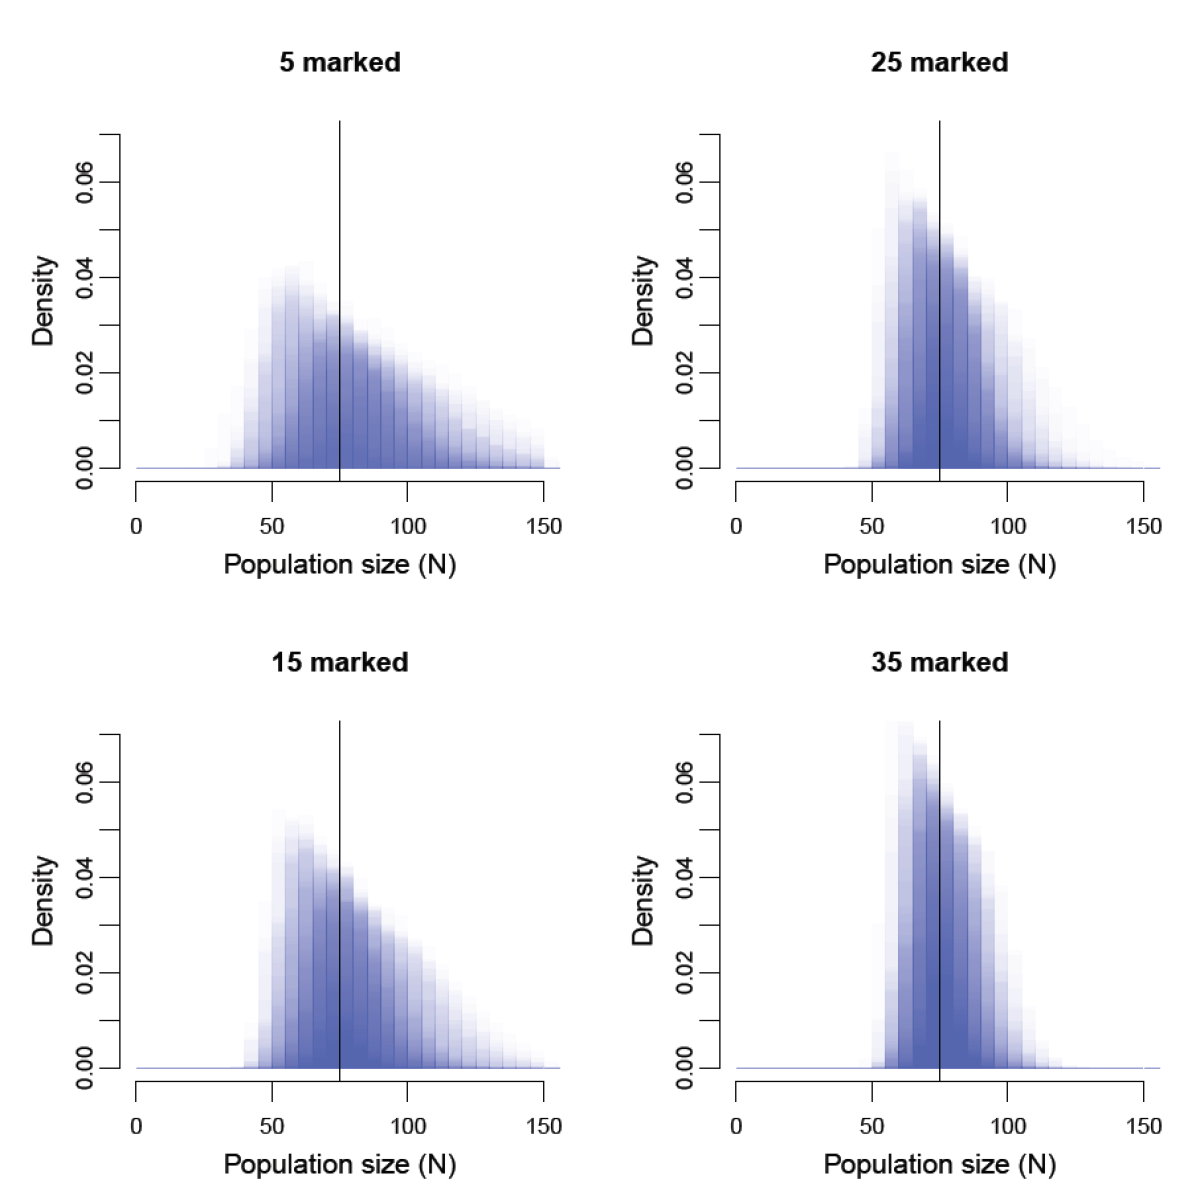
\includegraphics[width=4in,height=4in]{Ch19-PartialID/figs/Nposts2.png}
  \caption{Overlaid posterior distributions of $N$ from 100 simulations
    for four levels of marked individuals.}
  \label{partialID.fig.nposts}
\end{figure}

Without any marked individuals in the population, the posterior
distribution of $N$ turned out to be highly skewed, but the mode was
still an approximately (frequentist) unbiased point estimator of
$N$. As anticipated, posterior precision increased substantially with
the proportion of marked individuals (Table \ref{partialID.tab.sim} and
Fig. \ref{partialID.fig.nposts}). The relative root-mean squared
error decreased from 0.246 when no individuals were marked to 0.085
when 35 individuals were marked
(Table \ref{partialID.tab.sim}). Coverage was nominal for all values of
$m$ and posterior skew greatly diminished with increasing $m$ (Table \ref{partialID.tab.sim}).


\begin{table}[ht]
\centering
\caption{Posterior mean, mode, and associated relative RMSE for simulations in
  which $m$ of $N$=75 individuals were marked. One hundred simulations of each case were conducted. Table taken from \citet{chandler_royle:2012} }
\begin{tabular}{llrrrrr}
     \hline
     &	Parameter    &	Mean   &	rRMSE  & Mode   & rRMSE &	BCI    \\
     \hline
 m=0 &	$N$          &	85.866 &    0.259 & 77.720 &    0.242 & 0.950  \\
     &	$\lambda_0$  &	0.506  &	0.180 &	0.488  &	0.182 &	0.960  \\
     &	$\sigma$     &	0.495  &	0.115 &	0.486  &	0.113 &	0.960  \\
     \hline
 m=5 &	$N$          &	80.898 &    0.184 & 76.360 &    0.182 & 0.970  \\
     &	$\lambda_0$  &	0.510  &    0.178 & 0.494  &    0.180 & 0.950  \\
     &	$\sigma$     &	0.496  &    0.089 & 0.488  &    0.086 & 0.970  \\
     \hline
 m=15&	$N$          &	79.028 &    0.148 & 76.250 &    0.147 & 0.950  \\
     &	$\lambda_0$  &	0.508  &    0.163 & 0.494  &    0.164 & 0.950  \\
     &	$\sigma$     &	0.496  &    0.073 & 0.492  &    0.071 & 0.970  \\
     \hline
 m=25&	$N$          &	77.765 &    0.114 & 75.810 &    0.113 & 0.950  \\
     &	$\lambda_0$  &	0.511  &    0.153 & 0.498  &    0.157 & 0.950  \\
     &	$\sigma$     &	0.496  &    0.067 & 0.493  &    0.065 & 0.940  \\
     \hline
 m=35&	$N$          &	76.446 &    0.085 & 74.900 &    0.085 & 1.000  \\
     &	$\lambda_0$  &	0.513  &    0.142 & 0.501  &    0.144 & 0.950  \\
     &	$\sigma$     &	0.497  &    0.056 & 0.493  &    0.057 & 0.940  \\
 \hline
\end{tabular}
\label{partialID.tab.sim}
\end{table}

As we saw in the previous chapter, the spatial correlation in unmarked
counts can be sufficient to obtain estimates of movement and detection
parameters. However, only marked and thus identifiable individuals
provide us with direct information about these parameters and may well
dominate estimates.  To single out the contribution of marked and
unmarked individuals to parameter estimates, we re-ran the same
simulations but let $\sigma$ and $\lambda_0$ be updated based solely
on the data of marked individuals. Results are summarized in
Table \ref{partialID.tab.sim2}.  We see that if we update $\lambda_0$
and $\sigma$ based on marked individuals only, estimates of these
parameters are more biased and less precise. For estimates of $N$,
especially for $m$= 5 and $m$ = 15, we observe a stronger positive
bias, lower accuracy and considerably lower BCI coverage as compared
to when both marked and unmarked individuals contribute to parameter
estimates (Table \ref{partialID.tab.sim2}). Thus, unmarked individuals
do actually contribute noticeably to estimating model parameters.

\begin{table}[ht]
\centering
\caption{Posterior mean, mode, and associated relative RMSE for simulations in
  which $m$ of $N$=75 individuals were marked and unmarked individuals
  did not contribute to estimating $\lambda_0$ and $\sigma$.
  One hundred simulations of each case were conducted. }
\begin{tabular}{llrrrrr}
\hline
     &	Parameter    &	Mean   &	RMSE  &	Mode   &	RMSE &	BCI    \\
     \hline
 m=5 &	$N$          &	88.621 &	0.369 &	83.139 &	0.421 &	0.810  \\
     &	$\lambda_0$  &	1.255  &	1.247 &	0.606  &	1.148 &	0.950  \\
     &	$\sigma$     &	0.472  &	0.252 &	0.426  &	0.333 &	0.910  \\
     \hline
 m=15&	$N$          &	81.031 &	0.192 &	78.361 &	0.175 &	0.820  \\
     &	$\lambda_0$  &	0.535  &	0.281 &	0.476  &	0.284 &	0.970  \\
     &	$\sigma$     &	0.503  &	0.109 &	0.490  &	0.107 &	0.940  \\
     \hline
 m=25&	$N$          &	78.206 &	0.129 &	76.594 &	0.123 &	0.920  \\
     &	$\lambda_0$  &	0.531  &	0.204 &	0.496  &	0.202 &	0.960  \\
     &	$\sigma$     &	0.497  &	0.081 &	0.489  &	0.084 &	0.950  \\
     \hline
 m=35&	$N$          &	76.833 &	0.099 &	75.422 &	0.096 &	0.940  \\
     &	$\lambda_0$  &	0.528  &	0.192 &	0.505  &	0.186 &	0.940  \\
     &	$\sigma$     &	0.499  &	0.069 &	0.493  &	0.070 &	0.960  \\
 \hline
\end{tabular}
\label{partialID.tab.sim2}
\end{table}


\section{Incorporating telemetry data}
\label{partialID.sec.telemetry}

As we expected, parameter estimates of spatial mark-resight models get
better the more marked individuals we have in our study
population. While this is great advice in theory, it may not be very
helpful in practice, especially when dealing with animals that are
hard or somewhat dangerous to capture, such as large
carnivores. Oftentimes, studies involving the physical capture of such
animals will employ telemetry tags in order to learn about the study
species' spatial ecology and behavior. In the context of spatial
mark-resight models, the actual locations
collected by telemetry tags can provide detailed information on individual location and movement, and being able to incorporate this information directly into the SMR model should improve estimates of these parameters, especially when resighting information is sparse.

%% XXXXX Andy: seems like a cite to the JAPPLE paper would be good
%% around here?
% XX RS: We cite it in the last paragraph of this section. 

So how could we combine resighting data and telemetry data in a
unified mark-resight model? Recall that the basic SCR model underlying
all the SMR models we discuss here uses a Gaussian kernel to describe
the trap encounter model.  By using this function, we can relate the
parameters $\sigma$ and ${\bf s}_{i}$ directly to those from a
bivariate normal model of space usage, with mean = ${\bf s}_{i}$, and
variance-covariance matrix ${\bm \Sigma}$, where the variance in both
dimensions is $\sigma^2$ and the covariance is 0. Ordinarily, these
parameters are estimated directly from the spatial distribution of
individual captures/resightings. Telemetry data, however, provide more
detailed information on individual location and movement, since the
resolution and extent of the data are not limited by the trapping grid
and potentially more locations can be accumulated through telemetry
than resighting (depending on the monitoring frequency and resighting
rates of individuals).

By assuming that the $R_i$ locations of individual $i$, ${\bf l}_{i}$ (consisting of a pair of x and y coordinates, $l_{ix}$ and $l_{iy}$), are a bivariate normal (BVN) random variable:
\[
{\bf l}_i\sim {\mbox BVN} ({\bf s}_i,{\bm \Sigma})
\]
we can estimate $\sigma$ as well as ${\bf s}_{i}$ for the collared individuals directly from telemetry locations, using their full conditional distributions:
\[
[\sigma|{\bf l},{\bf s}] \propto \left\{\prod_{i=1}^m \prod_{r=1}^{R_{i}} \frac{1}{2 \pi \sigma^2} {\exp}\left(-1/2 \left[ \frac {(l_{irx}-s_{ix})^2} {\sigma^2} + \frac{(l_{iry}-s_{iy})^2}{\sigma^2} \right]\right)\right\}*[\sigma]
\]
and
\[
[{\bf s}_i|{\bf l},\sigma] \propto \left\{\prod_{r=1}^{R_{i}} \frac{1}{2 \pi \sigma^2} {\exp}\left(-1/2 \left[ \frac {(l_{irx}-s_{ix})^2} {\sigma^2} + \frac{(l_{iry}-s_{iy})^2}{\sigma^2} \right]\right)\right\}*[{\bf s}_{i}]
\]

For the unmarked individuals ${\bf s}_{i}$ are estimated as described
before conditional on their latent encounter histories.  Note that the
bivariate normal model assumes that locations are independent of each
other. If you have frequent telemetry fixes, for example from GPS
collars that report animal locations every few hours or more, this
assumption seems unrealistic and it might be advisable to thin your
telemetry data (maybe to daily fixes) in order to approximate
independence.  Alternatively, movement models could be used that
acknowledge the temporal correlation in location data. We suggested
some possible movement models in Chapt. \ref{chapt.search-encounter}.
Not all marked individuals need to be telemetry-tagged, but telemetry
data should correspond to the period over which resighting surveys
were conducted (as we discussed in Chapt. \ref{chapt.scr0}, both the
${\bf s}_i$ and $\sigma$ should only be interpreted against the
specific sampling period). Further, telemetry data need to be
independent of the resighting data.

Again, implementation of this model extension is straight-forward,
both in {\bf JAGS} and {\bf R}. Take the SMR model description for the
case where $m$ is known (Panel \ref{partialID.panel.knownm}). Then,
all we have to do is add a description of the bivariate normal model
for the telemetry locations, here {\tt locs}, into the loop over the
$m$ marked individuals: 
{\small
\begin{verbatim}
[...parts of model code omitted...]

for(i in 1:m) {

  sm[i,1] ~ dunif(xlim[1], xlim[2])
  sm[i,2] ~ dunif(ylim[1], ylim[2])

  #telemetry model
  for (r in off1[i]:off2[i]){
  locs[r,1]~dnorm(sm[i,1], 1/(sigma^2))
  locs[r,2]~dnorm(sm[i,2], 1/(sigma^2))
  }

  for(j in 1:J) {
    distm[i,j] <- sqrt((sm[i,1]-X[j,1])^2 + (sm[i,2]-X[j,2])^2)
    lambdam[i,j] <- lam0*exp(-distm[i,j]^2/(2*sigma^2))
    y[i,j]~dpois(lambdam[i,j]*K)
    }
  }

[...parts of model code omitted...]
\end{verbatim}
}
The data object {\tt locs} is a table with all $\sum_i^m R_i$
telemetry locations. The two vectors {\tt off1} and {\tt off2}
describe which subset of this matrix belongs to individual $i$. So if,
say, the locations for individual 1 are contained in the first 10 rows
of {\tt locs}, {\tt off1} and {\tt off2} would be 1 and 10 for $i=1$;
and if the locations of individual 2 are in the following 15 rows,{\tt
  off1} and {\tt off2} for $i=2$ would be 11 and 25, and so on. For
the implementation of this SMR model with telemetry data in {\bf R},
see the {\tt scrPID.tel} function in {\tt scrbook}. In a nutshell, in
the MCMC algirithm we replaced the Metropolis-Hastings updating steps
for $\sigma$ and activity centers, ${\bf s}_i$, of marked individuals, which were originally
conditional on the resighting data, with updating steps conditional on
the telemetry data. This is not quite what the above {\bf JAGS} code
does; rather {\bf JAGS} will update these parameters conditional on
both the telemetry \emph{and} the resighting data. We could easily
re-write {\tt scrPID.tel} to do that, but believe that for most
applications, the information on location and movement contained in
the telemetry data will outweigh that in the resighting data, so that
the resulting loss of information should be minimal.

\subsection{Raccoons on the Outer Banks of North Carolina}

\citet{sollmann_etal:2012ecol} applied a spatial mark-resigh model
with telemetry data to a camera-trap and radio-telemetry data set from
the raccoon population on South Core Banks, a barrier island within
Cape Lookout National Seashore, North Carolina. Between May and
September 2007, 131 raccoons were marked with dog collars and large
individually numbered cattle tags. Individuals were marked throughout
the island, so that (a) we do not have to deal with sensitivity to
choice of the state-space, because it is clearly defined by nature;
and (b) it is reasonable to assume that marked raccoons are a random
sample of individuals from this state-space.  Of the 131 tagged
individuals, 44 were also equipped with radio collars. Collared
individuals were located using a VHF receiver and antenna, and their
locations were estimated approximately weekly. Twenty camera traps
were set up along the length of South Core Banks and camera trapping
data collected between October 1 2007 to January 22 2008 constituted
the resighting data in this analysis. During this period 104 marked
individuals, 38 radio-collared, were alive and available for
resighting with camera traps.

\begin{figure}[ht]
  \centering
  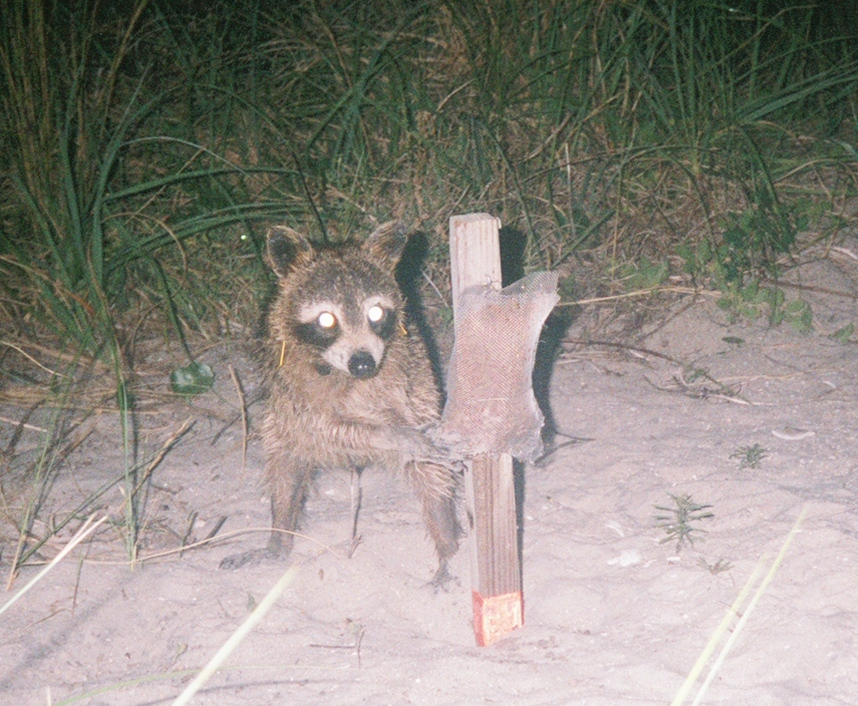
\includegraphics[width=4in]{Ch19-PartialID/figs/Raccoon_pic.png}
  \caption{Camera trap picture of a raccoon marked with a cattle tag that cannot be read to determine individual identity. Taken on South Core Banks, North Carolina.
({\it Photo credit: Arielle Parsons})}
  \label{partialID.fig.raccoon}
\end{figure}

The state-space ${\cal S}$ was the entire area of South Core Banks
island. A change in the number of photocaptures over the course of the
study suggested a variation of detection rate with time. Since date
recording in cameras malfunctioned, photographic records could only be
assigned to the time interval between subsequent trap checks, and
these intervals between checks are referred to as sampling
occasions. These occasions ranged from 2 to 43 days; $\lambda_0$ was
standardized to 7-day intervals and allowed to change with sampling
occasion. Since not all pictures of marked raccoons could be
identified to the individual level, the authors applied the correction
factor $c$ as described in Sec. \ref{partialID.sec.IDrate}, estimated
separately for each occasion.

Camera-traps recorded 117 pictures of unmarked raccoons, 33 pictures
of 18 marked and identifiable raccoons, and 49 records of marked but
not individually identifiable individuals
(Fig. \ref{partialID.fig.raccoon}). An average of 16.32 telemetry
locations (SD 4.91) were collected for each of the 38 collared
individuals. Raccoon abundance on the island was estimated at 186.71
(SE 14.81) individuals, which translated to a density of 8.29 (SE
0.66) individuals per km$^2$. Parameter estimates are listed in
Table \ref{partialID.tab.raccoons}.

\begin{table}%[hb]
\centering
\caption{Summary statistics of posterior distributions
from spatial mark-resigh model for raccoon camera trapping and telemetry data. Baseline trap encounter rate $\lambda_0$ was standardized to 7-day intervals; $\lambda_0$ and the probability of identifying a picture of a marked individual, $c$, were allowed to vary among the 6 sampling occasions (t); $\sigma$ is estimated from telemetry data of 38 radio-collared individuals.}
\begin{tabular}{lrrrrr}
\hline
   &	Mean (SE) &	2.5\% &	50\%	& 97.5\% \\
 \hline
$N$	& 186.71 (14.81) & 162 & 185	& 220 \\
$D$	& 8.29 (0.66)	& 7.19	& 8.22	& 9.77 \\
$\lambda_0$ (t=1)	& 0.24 (0.05) & 0.16 & 0.23 & 0.34 \\
$\lambda_0$ (t=2)	& 0.40 (0.08)	& 0.26	& 0.39	& 0.57 \\
$\lambda_0$ (t=3)	& 0.11 (0.03) & 0.06 & 0.11	& 0.17 \\
$\lambda_0$ (t=4)	& 0.30 (0.07)	& 0.17	& 0.29	& 0.46 \\
$\lambda_0$ (t=5)	& 0.03 (0.01)	& 0.02	& 0.03	& 0.06 \\
$\lambda_0$ (t=6)	& 0.03 (0.01)	& 0.02	& 0.03	& 0.05 \\
$\sigma$	& 0.49 (0.01)	& 0.47	& 0.49	& 0.51 \\
$c$ (t=1)	& 0.55 (0.09)	& 0.38	& 0.55	& 0.71 \\
$c$ (t=2)	& 0.39 (0.11)	& 0.18	& 0.39	& 0.62 \\
$c$ (t=3)	& 0.29 (0.11) & 0.11	& 0.29	& 0.52 \\
$c$ (t=4)	& 0.38 (0.16)	& 0.10	& 0.36	& 0.71 \\
$c$ (t=5)	& 0.38 (0.16)	& 0.10	& 0.36	& 0.71 \\
$c$ (t=6)	& 0.30 (0.14)	& 0.08	& 0.29	& 0.60 \\
 \hline
\end{tabular}
\label{partialID.tab.raccoons}
\end{table}

In this study, although a large number of raccoons were tagged,
photographic data of these tagged individuals were surprisingly
sparse. Analysis of the photographic data set without the telemetry
data did not render usable estimates as parallel Markov chains did not
converge. One reason for the relatively sparse data was the camera
trap study design: traps were spaced on average 1.77 km apart, which
is about 3.5 times $\sigma$. Consequently, very few individual
raccoons were photographed at more than one trap. Under these
circumstances, the telemetry data provide the necessary spatial
information to estimate $\sigma$ and the activity centers of
individual animals and thus make other model parameter
estimable. Similarly, in a camera-trapping study on Florida panthers
(\emph{Puma concolor coryi}), \citet{sollmann_etal:inprepjapplecol},
including telemetry data from the 3 individuals that were collared and
known to use the study area resulted in density estimates with
considerably higher precision as compared to preliminary estimates
\emph{without} telemetry location data, reducing the width of the 95
\% BCI by about 60 \%. Such improvements in precision of estimates is
especially important when we are interested in changes in the
population over time.


\section{Marked Animals Are Aot a Random Sample From the State-Space}

As discussed in Sec. \ref{partialID.sec.random}, all the previously
developed SMR models assume that marked individuals are a random
sample, both spatially and demographically, from the population of the
state-space. For many studies it may not be feasible to strive to meet
or approximate this assumption and it is thus important to generalize
SMR models to situations where marking does not take place throughout
${\cal S}$. If you think about it, even if you set up marking traps
throughout the state-space, individuals at the border of ${\cal S}$
would be exposed to fewer traps and be less likely to be caught, thus
creating a gradient in the proportion of marked to unmarked animals
(although if ${\cal S}$ is large enough this is probably negligible).
% XXXX RC: This last sentence doesn't seem to get at the key point,
% i.e. that the marked guys can almost never be assumed to be
% uniformly distributed in S.
%% Andy sez: but see my email from the morning of 3/24. Can you do a
%% random sample of traps and make a design-based argument here?
 Here, we will describe
%develop 
one tentative approach to dealing with this situation, by having marked individuals be a random (uniformly distributed) sample from a smaller region within ${\cal S}$, say ${\cal B}$.
The central point of this approach is that it establishes a spatial context for the marked part of the population. This spatial context is independent of ${\cal S}$ -- ${\cal B}$ remains constant -- and it provides a formal distribution of marked animals -- uniform in ${\cal B}$, none outside of ${\cal B}$ -- so that unmarked animals can be distributed in a way that overall density is constant.


\subsection{Marked animals are uniformly distributed in a smaller
  area}


%%% XXX Andy sez: not sure what to make of all of this.  By Richard's
%%% comments I gather that it is perhaps too experimental at this
%%% point. Can it be thinned down a bit to not say too much?

Imagine we perform an area search in a square, ${\cal B}$, for some species we want to study, maybe a reptile, and we mark all individuals we encounter. We conduct our sampling in a way that we can assume that the individuals we marked are uniformly distributed in ${\cal B}$. This also entails the assumption that ${\cal B}$ can be clearly defined. We will come back to these assumptions in a minute. We then perform resighting surveys of some sort in an area that overlaps ${\cal B}$, so that, when we set a state-space around our resighting locations, ${\cal B}$ is completely contained within ${\cal S}$ (Fig. \ref{partialID.fig.Box}), and we assume that the number of marked animals, $m$, is known. We further assume that individuals that were marked in ${\cal B}$ continue to live within ${\cal B}$ when resighting surveys are conducted, i.e. their activity centers do not shift during the complete mark-resight study. That means that we assume population closure across both the marking and the resighting part of the study.
% XXXX RC: This also assumes that there are no marked activity centers outside of B, which I think will be impossible and should be mentioned... again.

Let the total population of ${\cal B}$ be $N_B$. % XXXX Suggest: $N({\cal B})$?
% XXXX After defining N(B), I would establish that, under the
% assumption that of uniform *marginal* density, the expected values
% for each N are as follows (when using data augmentation):
% E[N] = M*psi
% E[N marked guys in B] = M*psi*theta
% E[N unmarked guys in B] = M*psi*(1-theta)
% E[N unmarked gusy outside of B] = M*psi*pi, where pi is (A(S)-A(B))/A(S)
Under the conditions specified above, the number of marked animals $m$ can be described as the outcome of a binomial random variable
\[
m \sim \mbox{Binomial}(\theta, N_B)
\]
where $\theta$ is the probability that an animal living in ${\cal B}$ is marked. Remember that, by definition, all marked animals live inside ${\cal B}$. We now have to make sure that unmarked individuals get distributed across ${\cal S}$ and ${\cal B}$ so that \emph{overall} density is constant. % XXXX RC: I think this should be stated as a (possibly) reasonable assumption, instead of something that "we have to make sure" is true
Let ${\cal A}$ be ${\cal S} - {\cal B}$, % XXXX RC: instead of a "minus" sign, I think you want $S \ni B$ or whatever the appropriate geometric symbol is.
i.e., the area of ${\cal S}$ \emph{not} covered by ${\cal B}$ (Fig. \ref{partialID.fig.Box}). Then, the proportion of $N$ that should fall inside ${\cal B}$, say $\pi_B$, can be expressed as ${\cal B}/({\cal A}+{\cal B})$. Consequently, the proportion of $N$ in ${\cal A}$, $\pi_A$,
% XXXX RC: You need to distinguish between S and the area of S, which could be denoted A(S) or something.
is ${\cal A}/({\cal A}+{\cal B})$.
Conditioning $\pi_B$ on being an unmarked animal, % XXXX RC: rephrase
we obtain
\[
 \pi_B | unmarked = \frac{(1-\theta)* \pi_B}{U/N}
\]
And we can use this conditional probability as prior probability for the activity centers of unmarked individuals to fall within {\cal B}.
In other words, we now have two sets of priors for activity centers.
% XXXX RC: I don't think this is the prior for activity centers. Under
% this model, all the activity centers have a uniform prior, but
% density is different for the 3 groups. That is why I would focus on
% the expected values of N that I listed above.
For marked animals, $[s_i]\sim \mbox{Uniform}({\cal B})$. For unmarked animals, we introduce a binary variable, say $b$, and let $b=1$ mean that $s_i$ lies within ${\cal B}$; then $[s_i]\sim \mbox{Bernoulli}(pi_B|unmarked)$.
Because manipulating areas that are not simple rectangles (in this example, ${\cal A}$) in {\bf JAGS} is not straight forward, we wrote our own MCMC algorithm for this model, which can be found in the {\tt scrbook} package by invoking {\tt scrPIDBox}. A full example of how to simulate and analyze data under this model is given on the help page for {\tt scrPIDBox}.

\begin{figure}[ht]
\begin{center}
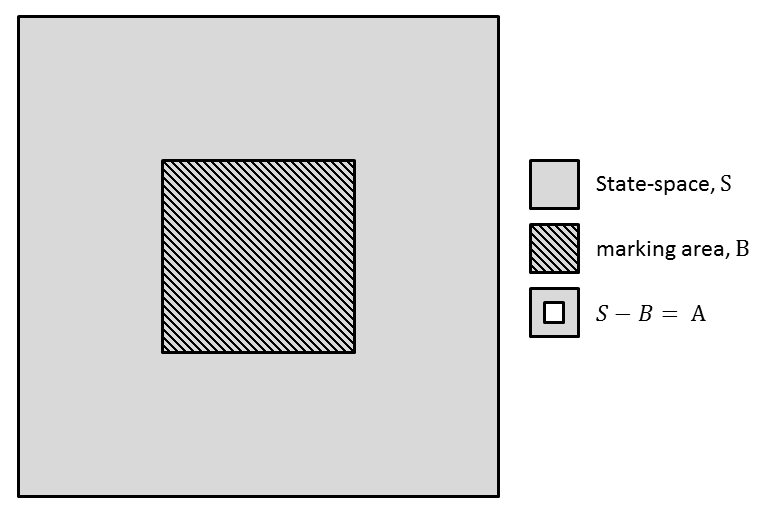
\includegraphics[width=5in]{Ch19-PartialID/figs/scrPIDBox.png}
\end{center}
\caption{
Relationship between marking area ${\cal B}$ and state-space, ${\cal S}$.
}
\label{partialID.fig.Box}
\end{figure}

The above %described
model is an approach to specifying a spatial reference frame for
marked individuals if these are not sampled uniformly from ${\cal S}$,
and provides us with the ability to distribute unmarked individuals
% XXXX RC: This reads as though "we" are distributing unmarked
% individuals around in space. I think it should say that this is a
% model that is reasonable if overall density can be assumed to be
% constant and the activity centeres of the marked guys are all
% uniformly distriubted within B.
proportionally between the marking area and the rest of the state-space, so that an overall uniform density is obtained. Some of the assumptions of the model, however, are reminiscent of traditional capture-recapture and thus, suffer from the same shortcomings. ${\cal B}$ needs to be clearly defined as the area the marked individuals live in, but how do we define it? Imagine again that ${\cal B}$ is a quadrad search plot. Surely, we could capture an individual at the edge of the plot, whose activity center is located \emph{off} that plot. Not accounting for this effect would overestimate density in ${\cal B}$. This is the equivalent of  having to define an effective area sampled in traditional capture-recapture in order to estimate density. Further, we assume that $\theta$, the probability of an individual within the plot being marked is the same for all individuals in ${\cal B}$. But we discussed early on in this book that this is unlikely to be true, because exposure to sampling depends on an individual's home range overlap with the sampled area. So individuals near the edge of ${\cal B}$ are less likely to be marked than those in the center, assuming we dispense marking effort uniformly across ${\cal B}$ (maybe we could counteract this effect to some extent by creating a decreasing gradient of sampling effort from the edge of the plot to the center).

\subsection{Combining marking and resighting models}

% XXXX I would remove this section, and instead focus on the solution
% that we know works: develop a model for spatial variation in the
% density of marked guys. We know this works because you imagine
% ignoring all of the unmarked guys and just estimating the abundance/density of
% marked guys. In that case, the only thing that differs from a
% standard SCR model is that we need to use an inhomogeneous point
% process because the marked guys will not be uniformly distributed in
% S. Istead, their density will almost surely decrease with distance
% from the traps where they were marked. There are several different
% ways of modeling this decrease in density. Once that is done, the
% IPP for the unmarked guys can be modeled by assuming that overall
% density is constant. Even if it isn't, you could theoretically
% develop any IPP for the unmarked guys too.

We can look at this approach from a slightly different
angle. Effectively, what we did here is combine a non-spatial capture
recapture model -- more specifically, model $M_0$ with equal capture
probability -- for the marking process with a spatial mark-resight
model for the resighting process. In our simplified example, we only
have a single marking occasion, but we can estimate $\theta$, the
probability of being captured and marked, because we have enough
information about how many unmarked individuals occur in ${\cal B}$
coming from the spatial resighting model. While the underlying
assumptions of the non-spatial marking model are questionable, we
believe that the idea of combining marking and resighting into a
unified model holds the key to developing a generalized spatial
mark-resight model that does not rely on animals being marked
throughout ${\cal S}$, at least when marking and resighting occur in a
short enough time frame that the population can be assumed closed. As
such, in spite of some shortcomings, the present approach is an
important conceptual step forward. We can think of alternative
distributions for marked individuals to move away from a completely
non-spatial description of the marking process; for example, activity
centers of marked individuals could follow a bivariate normal
distribution around the centroid of the marking array or plot, so that
the probability of being a marked individual is conditional on where
you live and decreases with distance to the collection of marking
locations. This avoids having to arbitrarily define an area, ${\cal
  B}$, but is still a simplification of the actual marking process. We
have not yet implemented this approach.  The essence of all of this is
that including the marking process into an SMR model provides a
spatial context for marked individuals, so that the resighting part of
the model is no longer sensitive to the choice of the state-space. The
next steps will be to develop a fully spatial model, where both the
marking and the resighting process are spatially explicit, and to
extend these models to the situation we can no longer use the
information from the marking process directly to provide spatial
context for marked individuals, because too much time passed between
marking individuals and resighting them, so that the assumption that
activity centers remain stationary is no longer reasonable.


%\subsection{Marked animals follow a bivariate normal distribution around the centroid of the marking array}
% In this approach we assume that marking of animals takes place across some area and that in the time between marking and resighting, the marked animals, the number of which is unknown, distribute themselves according to a bivariate normal distribution centered on the centroid of the marking area or grid, say $C_m$. This could happen in two fashions: (a) animals spread out around the marking area, but most stay close while only few venture out further; or (b) this represents the original distribution of marked animals, because animals living in the center of the markign grid have a higher probability to be marked than those living on the edges, so that the density of marks is higher near the centriod of the marking grid and decreases (here, following a bivariate normal distribution) as we move a away from that centroid.
% This model allows us to describe the probability of an animal being marked as a function of the distance of its activity center to $C_m$




\section{Summary and Outlook}

In this chapter we combined SCR models and the spatial model for
unmarked populations to derive a spatial mark-resight model, which
accomodates that part of the population is individually identifiable,
usually through artificial tags. Under the assumption that marked
individuals are a random sample, both demographically and spatially,
from the state-space, the basic model with known number of marked
individuals and 100\% individual identification of marked is easily
modified for situations where the number of marked individuals is
unknown, or where marked animals can sometimes not be identified to
individual level. As expected, having marked individuals in the study
population improved accuracy and precision of parameter estimates when
compared to fully unmarked populations, but we also saw that the
spatial counts of unmarked individuals still contribute information to
parameter estimates. Finally, we present an approach of how to
incorporate telemetry location data into the spatial mark-resight
model to inform estimates of $\sigma$ and activity centers. Just as in
SCR, the spatial mark-resight models can account for a variety of
factors that may influence individual movement and detection, as well
as survey-related parameters, and we saw one example for the Canada
geese, where $\sigma$ was sex-specific.

Many details of SMR models remain to be explored. We mentioned the
assignment of marked but unidentified records to actual marked
individuals based on their spatial location, which provides some
(though imperfect) information of their identity
(Sec. \ref{partialID.sec.IDrate}). Similarly, records where the marked
status cannot be determined could potentially be included in the model
as some form of overall correction factor on detection. GPS telemetry
devices and their ability to collect location data with much higher
frequency offer the opportunity to assign records of collared animals
to individuals based on how close to a given camera the collared
individuals were, both in space and time. In this scenario, individual
identity itself could be expressed probabilistically, leading to an
SMR model accounting for potential misidentification. All these
possible extensions can tailor SMR models to specific survey
techniques.

A fundamental assumption of all the SMR models developed in this chapter was that marked animals are a
random sample from ${\cal
  S}$. This simplifies the model as we can assume a homogeneous point process for both the marekd and the unmarked part of the population. While this is a convenient situation, it is neither likely to arise often in real life, nor a necessary assumption.  
If marked animals are not a random sample from
${\cal S}$, we need to describe their distribution in the state-space using an adequate point-process that will almost always be inhomogeneous across ${\cal S}$. 
We mention two possible approach -- a uniform (homogeneous) point process over a smaller area within ${\cal S}$, and a bivariate normal distribution around the centroid of the marking locations, so that density of marked animals decreases with distance to that centroid. 

Both formulations effectively attempt to describe the distribution of marks in space as a consequence of the spatial nature of the marking process. We believe that another way to approach this problem is to combine spatially explicit models for the marking process and the resighting process. Where  marked animals were captured carries information on their spatial distribution, and it should be possible to make use of this information by formulating an integrated spatial capture-mark-resighting model. Such approaches have been developed in a non-spatial CR framework \citep{matechou_etal:2013, pledger_etal:2009}, but to our knowledge have not yet been addressed in the context of SCR.

 Spatial mark-resight models are a fairly
new development and work on how to relax the spatial component of the
random sample assumption and formulate adequate point-process models for the distribution of marks is ongoing. While there is still a lot of work to be done, we believe that SMR modeling holds the
potential to address a wide range of population estimation problems
when dealing with animals that cannot be identified based on natural
marks.



% \subsection{Sensitivity to the state-space}

% While the formulation of spatial mark-resight models for a known
% number of marked indivduals, $m$, is straight forward, these model
% have one major caveat: because we fix the size of the marked part of
% our population, total population size $N$ no longer scales with the
% area of the state-space. While the number of unmarked individuals can
% go up as ${\cal S}$ increases in size, $m$ is fixed by design. If our
% data contain all-zero encounter histories for some of the marked
% individuals, we have no immediate information about where in the
% state-space these never observed individuals live (apart from the
% vague information that they probably do not live in the middle of the
% trap array). As we increase ${\cal S}$, the area over which these marked
% unobserved individuals can live increases, too -- and consequently,
% their density decreases.  As a result, we find that density estimates
% from spatial mark-resight models with a known number of marks are
% sensitive to choice of the state-space -- as we increase ${\cal S}$,
% density estimates go down.  This is, of course, a highly undesirable
% quality in a density model. {\bf XXXXX Not a property of the model,
%   but rather of misspecifying something! We need to figure this
%   out.... XXXXXX}
% While this is an area of active research,
% we believe that under certain circumstances, the problem of
% sensitivity to the state-space can be avoided: If all marked animals
% are resighted at least once, we have some information about where in
% the state-space they live -- their activity centers must be close
% enough to the trap array for them to be resighted on it. Thus, even if
% we increase the overall state-space, the possible locations for the
% activity centers of the marked individuals remain limited. The effect
% is that, irrespective of the state-space, the marked individuals refer
% to a constant area, instead of getting `diluted'. Even if marked
% individuals are not resighted, we might have other sources of
% information on where they resided during our study, such as telemetry
% locations. Again, this information gives us the ability to fix the
% area the marked individuals refer to irrespective of the size of ${\cal
%   S}$, avoiding bias in density estimates. For an example of how to
% include telemetry data into spatial mark-resight models, see
% Sec. \ref{partialID.sec.telemetry}. A third option that we have not
% formally explored ourselves is to explicitly include capture locations
% of marked individuals into the model. Once again, this would provide
% some spatial reference for the location of marked individuals within
% the state-space. Lastly, there are circumstances under which we know
% the exact state-space in which individuals were marked and are being
% resighted. For example, if we study the population of some species on
% an island, and the entire island's population is potentially exposed
% to marking efforts (see the raccoon example in
% Sec. \ref{partialID.sec.telemetry}). In this case there is no
% arbitrariness in choosing ${\cal S}$ -- it is the island. If none of
% these avenues is an option, there is always the possibility of
% treating the number of marked individuals as unknown (see
% Sec. \ref{partialID.sec.unknown}), which might be more realistic under
% most field situations anyway. You should not that while we discussed
% the problem of underestimating density with an increase in
% state-space, there is also the opposite risk: if we choose ${\cal S}$
% too small so that it does not contain the activity centers of all of
% the marked individuals, but we assume, by fixing $m$, that they are
% all part of the population, we will overestimate density -- just as we
% would if we chose ${\cal S}$ too small in a regular SCR setting. All
% this just emphaizes what we already stated in Chapt. \ref{chapt.scr0}:
% the state-space is an integral part of your spatial capture-recapture
% (or mark-resight) model and some thought should go into specifying it
% adequately.

% \subsection{MCMC for a spatial mark-resight model}

% Implementing a spatial mark-resight model in {\bf JAGS} is not
% trivial, % XXXX See the "scratch" directory and the .jag files for
%          % some examples of working around this issue in JAGS
% since the program does not accept partially observed
% multivariate nodes (in this case the partially observed individual
% encounter histories which we model as coming from a multinomial
% distribution). Therefore, knowing how to write your own MCMC algorithm
% comes
% in
% handy. You will find that we only have to make relatively
% simple modifications to the MCMC code we developed for regular SCR models in
% Chapt. \ref{chapt.mcmc}.
% Essentially, since we observe individual detections for the marked part of the population, we have to update only the unobserved part of ${\bf Y}$, and
% modify the updating steps for $z_i$ and $\psi$, the parameters introduced by data augmentation, to reflect some
% contribution to our
% knowledge of these parameters from the $m$ marked individuals.

% First, we set up an array to hold ${\bf Y}$, fill the first $m$ rows
% of the array with the $m$ observed individual encounter histories,
% then update ${\bf Y}$ for the unknown individuals only (note that the
% code is set up so that $n_{jk}$ contains both pictures of marked {\bf
%   and} unmarked individuals at $j$ and $k$):


% {\small
% \begin{verbatim}
% # set up placeholders and create vectors for marked and unmarked
%  Y <- array(NA, c(M, J, K))
%     nMarked <- nrow(y)
%     marked <- rep(FALSE, M)
%         marked[1:nMarked] <- TRUE
%         Y[1:nMarked, , ] <- y
%     z[marked] <- 1
%     Ydata <- !is.na(Y)
%     for (j in 1:J) {
%         for (k in 1:K) {
%             if (y[j, k] == 0) {
%                 Y[, j, k] <- 0
%                 next
%             }
%             unmarked <- !Ydata[, j, k]
%             nUnknown <- n[j, k] - sum(Y[!unmarked, j,k])
%             if (nUnknown < 0)
%                 browser()
%             probs <- lam[, j] * z
%             probs <- probs[unmarked]
%             probs <- probs/sum(probs)
%             Y[unmarked, j, k] <- rmultinom(1, nUnknown, probs)
%         }
%     }
% \end{verbatim}
% }

% When we know the number of marked individuals in the population estimating $N$ is reduced to etimating $U$. Thus, we only need to estimate the $z_i$ for $M-m$ unknown individuals and the updater for $z_i$ becomes:
% {\small
% \begin{verbatim}
% zUps <- 0
% seen <- apply(Y > 0, 1, any)
%    for (i in 1:M) {
%        if (seen[i] | marked[i])
%                 next
%        zcand <- ifelse(z[i] == 0, 1, 0)
%        ll <- sum(dpois(Y[i, , ], lam[i, ] * z[i], log = TRUE))
%        llcand <- sum(dpois(Y[i, , ], lam[i, ] * zcand,
%                   log = TRUE))
%        prior <- dbinom(z[i], 1, psi, log = TRUE)
%        prior.cand <- dbinom(zcand, 1, psi, log = TRUE)
%           if (runif(1) < exp((llcand + prior.cand) - (ll +
%                 prior))) {
%           z[i] <- zcand
%           zUps <- zUps + 1
%             }
%         }
% \end{verbatim}
% }
% Observe that while we skip the update of $z_i$ for the ``seen'' individuals (where  {\tt seen=TRUE} for any individual observed at least once and {\tt seen=FALSE} otherwise), {\tt seen} is defined based on ${\bf Y}$ and ${\bf Y}$ is updated at each iteration, so the $z_i$ for the observed but unmarked individuals are still updated.

% Finally, our update for $\psi$ needs to reflect that we are effectively only estimating $U$. In the full conditional beta distribution we have to replace $M$ with $M-m$ and $\sum z$ with $\sum z -m$:
% {\small
% \begin{verbatim}
%   psi<-rbeta(1,1+sum(w[!marked]),1+sum(!marked)-sum(w[!marked]))
% \end{verbatim}
% }
% The remainder of the code is essentially identical to the MCMC code for regular SCR models we developed in Chapt. \ref{chapt.mcmc}.
% You can find the full MCMC code (including the modeling options we'll discuss in the following sections) in the accompanying {\bf R} package {\tt scrbook} by invoking {\tt scrPID}.

% \subsection{Binomial encounter model}
% So far, we have only worked with Poisson encounter models for
% partially identifiable or unmarked populations. When we use a
% Bernoulli model instead, we have to make some changes to how we update
% the latent $y_{ijk}$, to ensure that a hypothetical individual
% receives at most a single observation at a given trap and occasion
% from the pool of $n_{jk}$ pictures. Thus, we move from a multinomial
% model
% where the same individual could be drawn repeatedly, to a sampling
% without replacement model(an individual drawn once at $j$ and $k$
% cannot be drawn again). The resuting full conditional distribution of
% the latent encounter histories is called a multivariate hypergemetric
% distibution; here is how we implement this in our MCMC algorithm:

% {\small
% \begin{verbatim}
%  Y <- array(NA, c(M, J, K))
% #[...]
%     for (j in 1:J) {
%         for (k in 1:K) {
%             if (y[j, k] == 0) {
%                 Y[, j, k] <- 0
%                 next
%             }
%             unmarked <- !Ydata[, j, k]
%             nUnknown <- n[j, k] - sum(Y[!unmarked, j,k])
%             if (nUnknown < 0)
%                 browser()
%             probs <- lam[, j] * z
%             probs <- probs[unmarked]
%             probs <- probs/sum(probs)
%             Y[unmarked, j, k] <- 0
%             guys <- sample(which(unmarked), nUnknown, prob = probs)
%             Y[guys, j, k] <- 1
%         }
%     }
% \end{verbatim}
% }


% {\bf R} makes it easy to implement the update of $\sigma$ and ${\bf
%   s}_i$ based on telemetry data and the above described full
% conditionals within our existing MCMC algorithm. We replace the
% current updating step for $\sigma$ with:
% {\small
% \begin{verbatim}
% #ntot = number of telemetry-tagged individuals
% #locs = list of length ntot; each element is a matrix
% #with telemetry locations
% #telID = vector with identifier for telemetry-tagged
% #individuals

% sigma.cand <- rnorm(1, sigma, delta[1])
% if (sigma.cand > 0) {

% llsig<-llsig.cand<-rep(NA, ntot)

% for (x in 1:ntot) {
% lls[x]<-sum(dmvnorm(x=locs[[x]],mean=c(S[telID[x],1],S[telID[x],2]),
% 			sigma=cbind(c(sigma^2,0), c(0,sigma^2)), log=T))
% lls.cand[x]<-sum(dmvnorm(x=locs[[x]],mean=c(S[telID[x],1],S[telID[x],2]),
% 	sigma=cbind(c(sigma.cand^2,0), c(0,sigma.cand^2)), log=T))
% 	}
%    if(runif(1) < exp( sum(lls.cand)  - sum(lls) ) ){
%     sigma<-sigma.cand
%     lam <- lam0*exp(-(D*D)/(2*sigma.cand*sigma.cand))
% 					}
% 			}
% \end{verbatim}
% }
% For the ${\bf s}_i$ we use an analogous updater for the
% telemetry-tagged individuals and the regular updater for individuals
% without associated telemetry location information.
% A full example can
% be found in the {\bf R} package {\tt scrbook}, by calling {\tt
%   scrPID.tel}.



% Further, if our data contain all-zero encounter histories
% for some of the marked individuals, we have no immediate information
% about where in the state-space these never observed individuals live
% (apart from the vague information that they probably do not live in
% the middle of the trap array). As we increase ${\cal S}$, the area
% over which these marked unobserved individuals can live increases, too
% -- and consequently, their density decreases. Even if we do not know
% $m$, we usually know an upper bound for it -- the total number ever
% caught before resighting. This upper bound does not change, no matter
% the size of the state-space, so again, at some point, estimates of $m$
% will hit the upper limit and after that, density will decrease as we
% increase ${\cal S}$. There is also the opposite risk: if we choose
% ${\cal S}$ too small so that it does not contain the activity centers
% of all of the marked individuals, but we assume, by fixing $m$, that
% they are all part of the population, we will overestimate density --
% just as we would if we chose ${\cal S}$ too small in a regular SCR
% setting. But this problem can be avoided much more easily, by
% increasing ${\cal S}$.









\bibliography{AndyRefs_alphabetized}

\end{document}